\PassOptionsToPackage{unicode=true}{hyperref} % options for packages loaded elsewhere
\PassOptionsToPackage{hyphens}{url}
\PassOptionsToPackage{dvipsnames,svgnames*,x11names*}{xcolor}
%
\documentclass[a4paper,]{book}
\usepackage{lmodern}
\usepackage{amssymb,amsmath}
\usepackage{ifxetex,ifluatex}
\usepackage{fixltx2e} % provides \textsubscript
\ifnum 0\ifxetex 1\fi\ifluatex 1\fi=0 % if pdftex
  \usepackage[T1]{fontenc}
  \usepackage[utf8]{inputenc}
  \usepackage{textcomp} % provides euro and other symbols
\else % if luatex or xelatex
  \usepackage{unicode-math}
  \defaultfontfeatures{Ligatures=TeX,Scale=MatchLowercase}
\fi
% use upquote if available, for straight quotes in verbatim environments
\IfFileExists{upquote.sty}{\usepackage{upquote}}{}
% use microtype if available
\IfFileExists{microtype.sty}{%
\usepackage[]{microtype}
\UseMicrotypeSet[protrusion]{basicmath} % disable protrusion for tt fonts
}{}
\IfFileExists{parskip.sty}{%
\usepackage{parskip}
}{% else
\setlength{\parindent}{0pt}
\setlength{\parskip}{6pt plus 2pt minus 1pt}
}
\usepackage{xcolor}
\usepackage{hyperref}
\hypersetup{
            colorlinks=true,
            linkcolor=Maroon,
            filecolor=Maroon,
            citecolor=Blue,
            urlcolor=Blue,
            breaklinks=true}
\urlstyle{same}  % don't use monospace font for urls
\usepackage[a4paper]{geometry}
\usepackage{color}
\usepackage{fancyvrb}
\newcommand{\VerbBar}{|}
\newcommand{\VERB}{\Verb[commandchars=\\\{\}]}
\DefineVerbatimEnvironment{Highlighting}{Verbatim}{commandchars=\\\{\}}
% Add ',fontsize=\small' for more characters per line
\usepackage{framed}
\definecolor{shadecolor}{RGB}{255,255,255}
\newenvironment{Shaded}{\begin{snugshade}}{\end{snugshade}}
\newcommand{\AlertTok}[1]{\textcolor[rgb]{0.75,0.01,0.01}{\textbf{\colorbox[rgb]{0.97,0.90,0.90}{#1}}}}
\newcommand{\AnnotationTok}[1]{\textcolor[rgb]{0.79,0.38,0.79}{#1}}
\newcommand{\AttributeTok}[1]{\textcolor[rgb]{0.00,0.34,0.68}{#1}}
\newcommand{\BaseNTok}[1]{\textcolor[rgb]{0.69,0.50,0.00}{#1}}
\newcommand{\BuiltInTok}[1]{\textcolor[rgb]{0.39,0.29,0.61}{\textbf{#1}}}
\newcommand{\CharTok}[1]{\textcolor[rgb]{0.57,0.30,0.62}{#1}}
\newcommand{\CommentTok}[1]{\textcolor[rgb]{0.54,0.53,0.53}{#1}}
\newcommand{\CommentVarTok}[1]{\textcolor[rgb]{0.00,0.58,1.00}{#1}}
\newcommand{\ConstantTok}[1]{\textcolor[rgb]{0.67,0.33,0.00}{#1}}
\newcommand{\ControlFlowTok}[1]{\textcolor[rgb]{0.12,0.11,0.11}{\textbf{#1}}}
\newcommand{\DataTypeTok}[1]{\textcolor[rgb]{0.00,0.34,0.68}{#1}}
\newcommand{\DecValTok}[1]{\textcolor[rgb]{0.69,0.50,0.00}{#1}}
\newcommand{\DocumentationTok}[1]{\textcolor[rgb]{0.38,0.47,0.50}{#1}}
\newcommand{\ErrorTok}[1]{\textcolor[rgb]{0.75,0.01,0.01}{\underline{#1}}}
\newcommand{\ExtensionTok}[1]{\textcolor[rgb]{0.00,0.58,1.00}{\textbf{#1}}}
\newcommand{\FloatTok}[1]{\textcolor[rgb]{0.69,0.50,0.00}{#1}}
\newcommand{\FunctionTok}[1]{\textcolor[rgb]{0.39,0.29,0.61}{#1}}
\newcommand{\ImportTok}[1]{\textcolor[rgb]{1.00,0.33,0.00}{#1}}
\newcommand{\InformationTok}[1]{\textcolor[rgb]{0.69,0.50,0.00}{#1}}
\newcommand{\KeywordTok}[1]{\textcolor[rgb]{0.12,0.11,0.11}{\textbf{#1}}}
\newcommand{\NormalTok}[1]{\textcolor[rgb]{0.12,0.11,0.11}{#1}}
\newcommand{\OperatorTok}[1]{\textcolor[rgb]{0.12,0.11,0.11}{#1}}
\newcommand{\OtherTok}[1]{\textcolor[rgb]{0.00,0.43,0.16}{#1}}
\newcommand{\PreprocessorTok}[1]{\textcolor[rgb]{0.00,0.43,0.16}{#1}}
\newcommand{\RegionMarkerTok}[1]{\textcolor[rgb]{0.00,0.34,0.68}{\colorbox[rgb]{0.88,0.91,0.97}{#1}}}
\newcommand{\SpecialCharTok}[1]{\textcolor[rgb]{0.24,0.68,0.91}{#1}}
\newcommand{\SpecialStringTok}[1]{\textcolor[rgb]{1.00,0.33,0.00}{#1}}
\newcommand{\StringTok}[1]{\textcolor[rgb]{0.75,0.01,0.01}{#1}}
\newcommand{\VariableTok}[1]{\textcolor[rgb]{0.00,0.34,0.68}{#1}}
\newcommand{\VerbatimStringTok}[1]{\textcolor[rgb]{0.75,0.01,0.01}{#1}}
\newcommand{\WarningTok}[1]{\textcolor[rgb]{0.75,0.01,0.01}{#1}}
\usepackage{longtable,booktabs}
% Fix footnotes in tables (requires footnote package)
\IfFileExists{footnote.sty}{\usepackage{footnote}\makesavenoteenv{longtable}}{}
\usepackage{graphicx,grffile}
\makeatletter
\def\maxwidth{\ifdim\Gin@nat@width>\linewidth\linewidth\else\Gin@nat@width\fi}
\def\maxheight{\ifdim\Gin@nat@height>\textheight\textheight\else\Gin@nat@height\fi}
\makeatother
% Scale images if necessary, so that they will not overflow the page
% margins by default, and it is still possible to overwrite the defaults
% using explicit options in \includegraphics[width, height, ...]{}
\setkeys{Gin}{width=\maxwidth,height=\maxheight,keepaspectratio}
\setlength{\emergencystretch}{3em}  % prevent overfull lines
\providecommand{\tightlist}{%
  \setlength{\itemsep}{0pt}\setlength{\parskip}{0pt}}
\setcounter{secnumdepth}{0}
% Redefines (sub)paragraphs to behave more like sections
\ifx\paragraph\undefined\else
\let\oldparagraph\paragraph
\renewcommand{\paragraph}[1]{\oldparagraph{#1}\mbox{}}
\fi
\ifx\subparagraph\undefined\else
\let\oldsubparagraph\subparagraph
\renewcommand{\subparagraph}[1]{\oldsubparagraph{#1}\mbox{}}
\fi
\pagestyle{headings}

% set default figure placement to htbp
\makeatletter
\def\fps@figure{htbp}
\makeatother

% mystylefile.pandoc
\usepackage[Lenny]{fncychap}
\usepackage{fancyhdr}
\pagestyle{fancy}
\fancyhf{}
\fancyhead[LE,RO]{\thepage}
\fancyhead[RE]{\leftmark}
\fancyhead[LO]{\rightmark}
\usepackage{tcolorbox}
\newtcolorbox{myquote}{colback=red!5!white, colframe=red!75!black}
\newtcolorbox{myverbatim}{colback=green!5!white, colframe=green!75!black}
% redefine the 'quote' environment to use this 'myquote' environment
\renewenvironment{quote}{\begin{myquote}}{\end{myquote}}

\usepackage{etoolbox}
\makeatletter
\patchcmd{\@verbatim}
  {\verbatim@font}
  {\verbatim@font\small}
  {}{}
\makeatother
  


\renewenvironment{Shaded}{\begin{snugshade}\small}{\end{snugshade}}

\usepackage{caption}
\captionsetup{labelformat=empty, font={sl}}

% for background image
\usepackage[pages=some]{background}
\backgroundsetup{
scale=1,
color=black,
opacity=0.5,
angle=0,
contents={%
  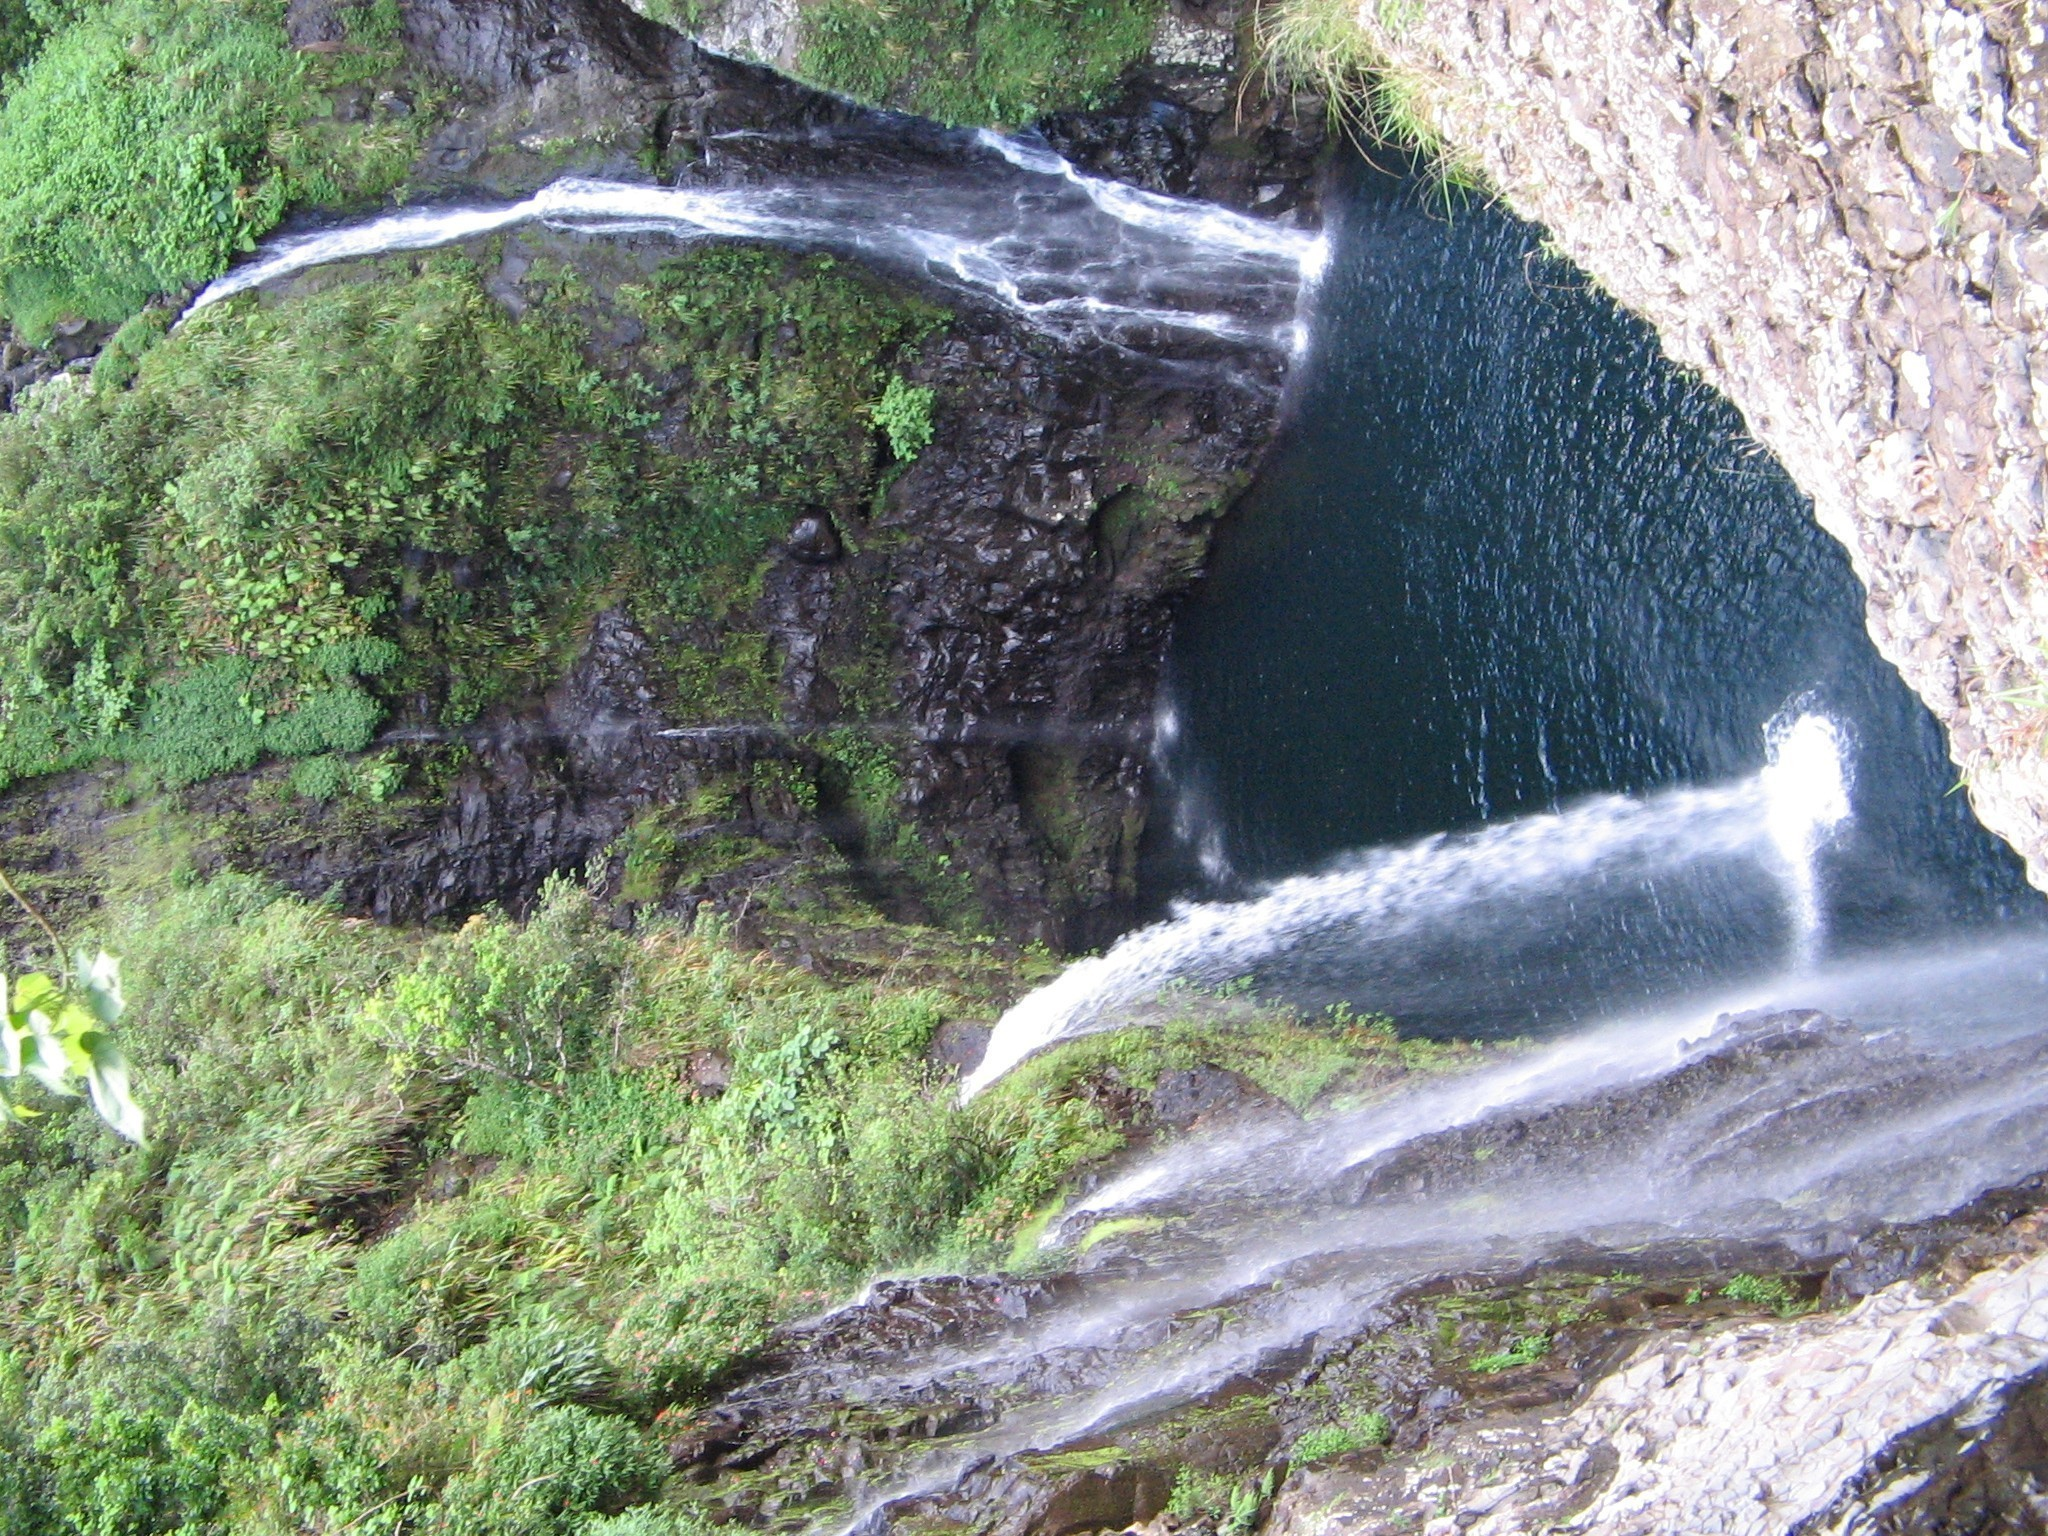
\includegraphics[width=\paperwidth,height=\paperheight,angle=-90]{pics/takamaka.jpg}
  }%
}

\begin{document}
\BgThispage
%% temporary titles
% command to provide stretchy vertical space in proportion
\newcommand\nbvspace[1][3]{\vspace*{\stretch{#1}}}
% allow some slack to avoid under/overfull boxes
\newcommand\nbstretchyspace{\spaceskip0.5em plus 0.25em minus 0.25em}
% To improve spacing on titlepages
\newcommand{\nbtitlestretch}{\spaceskip0.6em}
\pagestyle{empty}
\begin{center}
\bfseries
\nbvspace[1]
\Huge
{\nbtitlestretch\huge
PROGRAMMING HOTMOKA}

\nbvspace[1]
\normalsize

LEARN HOW TO PROGRAM SMART CONTRACTS\\
FOR BLOCKCHAIN APPLICATIONS\\
IN PURE JAVA
\nbvspace[1]
\small BY\\
\Large FAUSTO SPOTO\\[0.5em]
\footnotesize ASSOCIATE PROFESSOR\\
DEPARTMENT OF COMPUTER SCIENCE\\
UNIVERSITY OF VERONA, ITALY

\nbvspace[2]


\includegraphics[width=1in]{./pics/logo_minimal.png}
\nbvspace[3]
\normalsize

VERONA\\
\large
PUBLISHED IN THE WILD
\nbvspace[1]
\end{center}

\date{}



{
\hypersetup{linkcolor=}
\setcounter{tocdepth}{2}
\tableofcontents
}
\hypertarget{table-of-contents}{%
\begin{comment}\chapter{Table of Contents}\label{table-of-contents}}

\begin{enumerate}
\def\labelenumi{\arabic{enumi}.}
\tightlist
\item
  \protect\hyperlink{introduction}{Introduction}
\item
  \protect\hyperlink{installation}{Installation of Hotmoka}
\item
  \protect\hyperlink{first-program}{A First Program}

  \begin{itemize}
  \tightlist
  \item
    \protect\hyperlink{creation-eclipse-project}{Creation of the Eclipse
    Project}
  \item
    \protect\hyperlink{memory-blockchain}{Creation of a Hotmoka Node in
    Memory}
  \item
    \protect\hyperlink{jar-transaction}{A Transaction that Stores a Jar
    in a Hotmoka Node}
  \item
    \protect\hyperlink{logging}{Configuration of the Logging File}
  \item
    \protect\hyperlink{account-creation}{A Transaction that Creates an
    Account}
  \item
    \protect\hyperlink{using-views}{Using Views to Simplify the Code}
  \item
    \protect\hyperlink{constructor-transaction}{A Transaction that
    Creates an Object of our Program}
  \item
    \protect\hyperlink{method-transaction}{A Transaction that Invokes a
    Method}
  \item
    \protect\hyperlink{storage-types}{Storage Types and Constraints on
    Storage Classes}
  \item
    \protect\hyperlink{transactions}{Transactions Can Be Added, Posted
    and Run}
  \item
    \protect\hyperlink{tendermint}{Running on Tendermint}
  \end{itemize}
\item
  \protect\hyperlink{smart-contracts}{The Notion of Smart Contract}

  \begin{itemize}
  \tightlist
  \item
    \protect\hyperlink{simple-ponzi}{A Simple Ponzi Scheme Contract}
  \item
    \protect\hyperlink{fromcontract-payable}{The \texttt{@FromContract}
    and \texttt{@Payable} Annotations}
  \item
    \protect\hyperlink{payable-contracts}{Payable Contracts}
  \item
    \protect\hyperlink{view}{The \texttt{@View} Annotation}
  \item
    \protect\hyperlink{hierarchy-contracts}{The Hierarchy of Contracts}
  \item
    \protect\hyperlink{red-green-contracts}{Red/Green Contracts}
  \end{itemize}
\item
  \protect\hyperlink{support-library}{The Support Library}

  \begin{itemize}
  \tightlist
  \item
    \protect\hyperlink{storage-lists}{Storage Lists}

    \begin{itemize}
    \tightlist
    \item
      \protect\hyperlink{a-gradual-ponzi-contract}{A Gradual Ponzi
      Contract}
    \item
      \protect\hyperlink{a-note-on-re-entrancy}{A Note on Re-entrancy}
    \item
      \protect\hyperlink{running-the-gradual-ponzi-contract}{Running the
      Gradual Ponzi Contract}
    \end{itemize}
  \item
    \protect\hyperlink{storage_arrays}{Storage Arrays}

    \begin{itemize}
    \tightlist
    \item
      \protect\hyperlink{a-tic-tac-toe-contract}{A Tic-Tac-Toe Contract}
    \item
      \protect\hyperlink{a-more-realistic-tic-tac-toe-contract}{A More
      Realistic Tic-Tac-Toe Contract}
    \item
      \protect\hyperlink{running-the-tic-tac-toe-contract}{Running the
      Tic-Tac-Toe Contract}
    \item
      \protect\hyperlink{specialized-storage-array-classes}{Specialized
      Storage Array Classes}
    \end{itemize}
  \item
    \protect\hyperlink{storage_maps}{Storage Maps}

    \begin{itemize}
    \tightlist
    \item
      \protect\hyperlink{a-blind-auction-contract}{A Blind Auction
      Contract}
    \item
      \protect\hyperlink{events}{Events}
    \item
      \protect\hyperlink{running-the-blind-auction-contract}{Running the
      Blind Auction Contract}
    \item
      \protect\hyperlink{listening-to-events}{Listening to Events}
    \end{itemize}
  \end{itemize}
\item
  \protect\hyperlink{hotmoka-nodes}{Hotmoka Nodes}

  \begin{itemize}
  \tightlist
  \item
    \protect\hyperlink{publishing-a-hotmoka-node-online}{Publishing a
    Hotmoka Node Online}

    \begin{itemize}
    \tightlist
    \item
      \protect\hyperlink{publishing-a-hotmoka-node-on-amazon-ec2}{Publishing
      a Hotmoka Node on Amazon EC2}
    \end{itemize}
  \item
    \protect\hyperlink{building-a-hotmoka-remote-node-from-an-online-service}{Building
    a Hotmoka Remote Node from an Online Service}

    \begin{itemize}
    \tightlist
    \item
      \protect\hyperlink{creating-sentry-nodes}{Creating Sentry Nodes}
    \end{itemize}
  \item
    \protect\hyperlink{signatures-and-quantum-resistance}{Signatures and
    Quantum-Resistance}
  \end{itemize}
\item
  \protect\hyperlink{tokens}{Tokens}
\item
  \protect\hyperlink{code-verification}{Code Verification}

  \begin{itemize}
  \tightlist
  \item
    \protect\hyperlink{jvm-bytecode-verification}{JVM Bytecode
    Verification}
  \item
    \protect\hyperlink{takamaka-bytecode-verification}{Takamaka Bytecode
    Verification}
  \item
    \protect\hyperlink{command-line-verification-and-instrumentation}{Command-Line
    Verification and Instrumentation}
  \end{itemize}
\item
  \protect\hyperlink{references}{References}
\end{enumerate}

\end{comment}

\hypertarget{introduction}{%
\chapter{Introduction }\label{introduction}}

More than a decade ago, Bitcoin
\protect\hyperlink{Nakamoto08}{{[}Nakamoto08{]}} swept the computer
industry as a revolution, providing, for the first time, a reliable
technology for building trust over an inherently untrusted computing
infrastructure, such as a distributed network of computers. Trust
immediately translated into money and Bitcoin became an investment
target, exactly at the moment of one of the worst economical turmoil of
recent times. Central(-\emph{ized}) banks, fighting against the crisis,
looked like dinosaurs in comparison to the \emph{decentralized} nature
of Bitcoin.

Nevertheless, the novelty of Bitcoin was mainly related to its
\emph{consensus} mechanism based on a \emph{proof of work}, while the
programmability of Bitcoin transactions was limited due to the use of a
non-Turing-equivalent scripting bytecode
\protect\hyperlink{Antonopoulos17}{{[}Antonopoulos17{]}}.

The next step was hence the use of a Turing-equivalent programming
language (up to \emph{gas limits}) over an abstract store of key/value
pairs, that can be efficiently kept in a Merkle-Patricia trie. That was
Ethereum \protect\hyperlink{AntonopoulosW19}{{[}AntonopoulosW19{]}},
whose Solidity programming language allows one to code any form of
\emph{smart contract}, that is, code that becomes an agreement between
parties, thanks to the underlying consensus enforced by the blockchain.

Solidity looks familiar to most programmers. Conditionals, loops and
structures are there since more than half a century. Programmers assumed
that they \emph{knew} Solidity. However, the intricacies of its
semantics made learning Solidity harder than expected. Finding good
Solidity programmers is still difficult and they are consequently
expensive. It is, instead, way too easy to write buggy code in Solidity,
that \emph{seems} to work perfectly, up to \emph{that} day when things
go wrong, very wrong \protect\hyperlink{AtzeiBC17}{{[}AtzeiBC17{]}}.

It is ungenerous to blame Solidity for all recent attacks to smart
contracts in blockchain. That mainly happened because of the same
success of Solidity, that made it the natural target of the attacks.
Moreover, once the Pandora's box of Turing equivalence has been opened,
you cannot expect anymore to keep the devils at bay, that is, to be able
to decide and understand, exactly, what your code will do at run time.
And this holds for every programming language, past, present or future.

I must confess that my first encounter with Solidity was a source of
frustration. Why was I expected to learn another programming language?
and another development environment? and another testing framework? Why
was I expected to write code without a support library that provides
proved solutions to frequent problems? What was so special with Solidity
after all? Things became even more difficult when I tried to understand
the semantics of the language. After twenty-five years of studying and
teaching programming languages, compilation, semantics and code analysis
(or, possibly, just because of that) I still cannot explain exactly why
there are structures and contracts instead of a single composition
mechanism in Solidity; nor what is indeed the meaning of \texttt{memory}
and \texttt{storage} and why it is not the compiler that takes care of
such gritty details; nor why externally owned accounts are not just a
special kind of contracts; nor why Solidity needs such low-level (and
uncontrollable) call instructions, that make Java's (horrible)
reflection, in comparison, look like a monument to clarity; nor why
types are weak in Solidity, so that contracts are held in
\texttt{address} variables, whose actual type is unknown and cannot be
easily enforced at run time
\protect\hyperlink{CrafaPZ19}{{[}CrafaPZ19{]}}, with all consequent
programming monsters, such as unchecked casts. It seems that the
evolution of programming languages has brought us back to C's
\texttt{void*} type.

Hence, when I first met people from Ailia SA in fall 2018, I was not
surprised to realize that they were looking for a new way of programming
smart contracts over the new blockchain that they were developing. I
must thank them and our useful discussions, that pushed me to dive in
blockchain technology and study many programming languages for smart
contracts. The result is Takamaka, a Java framework for writing smart
contracts. This means that it allows programmers to use a subset of Java
for writing code that can be installed and run in blockchain.
Programmers will not have to deal with the storage of objects in
blockchain: this is completely transparent to them. This makes Takamaka
completely different from other attempts at using Java for writing smart
contracts, where programmers must use explicit method calls to persist
data to blockchain.

Writing smart contracts in Java entails that programmers do not have to
learn yet another programming language. Moreover, they can use a
well-understood and stable development platform, together with all its
modern tools. Programmers can use features from the latest versions of
Java, such as streams and lambda expressions. There are, of course,
limitations to the kind of code that can be run inside a blockchain. The
most important limitation is that programmers can only call a portion of
the huge Java library, whose behavior is deterministic and whose methods
are guaranteed to terminate.

Takamaka is included in the Hotmoka project, a framework for
collaborating nodes, whose long-term goal is to unify the programming
model of blockchain and internet of things. The more scientific aspects
of Takamaka have been published in the last years
\protect\hyperlink{Spoto19}{{[}Spoto19{]}}\protect\hyperlink{Spoto20}{{[}Spoto20{]}}.

\textbf{Acknowledgments}. I thank the people at Ailia SA, in particular
Giovanni Antino, Mario Carlini, Iris Dimni and Francesco Pasetto, who
decided to invest in this project and who are building their own
blockchain that can be programmed in Takamaka. My thank goes also to all
students and colleagues who have read and proof-checked this document
and its examples, finding bugs and inconsistencies; in particular to
Luca Olivieri and Fabio Tagliaferro. Chapter
\protect\hyperlink{hotmoka-nodes}{Hotmoka Nodes} is a shared work with
Dinu Berinde.

\emph{Verona, August 2020}.

\hypertarget{installation-of-hotmoka}{%
\chapter{Installation of Hotmoka }\label{installation-of-hotmoka}}

Takamaka is part of the Hotmoka project. The compiled jars of the
Hotmoka and Takamaka projects are not yet available on a public
repository such as Maven Central. Hence, the simplest way for using
Takamaka is to clone and install the Hotmoka project inside your local
Maven repository. You need Java JDK version at least 11 for compiling
the Hotmoka project.

Clone the project with:

\begin{myverbatim}
\begin{verbatim}
$ git clone git@github.com:Hotmoka/hotmoka.git
\end{verbatim}
\end{myverbatim}

then \texttt{cd} to the \texttt{hotmoka} directory and compile, package,
test and install the Hotmoka jars:

\begin{myverbatim}
\begin{verbatim}
$ mvn clean install
\end{verbatim}
\end{myverbatim}

If you want to generate the JavaDocs as well, you can use the following
Maven incantation instead:

\begin{myverbatim}
\begin{verbatim}
$ JAVA_HOME=/usr/lib/jvm/default-java mvn clean install javadoc:aggregate-jar
\end{verbatim}
\end{myverbatim}

placing, after \texttt{JAVA\_HOME=}, the correct path inside your
computer (which might not be that reported in the example above),
pointing to your Java installation directory.

In both cases, all tests should pass and all projects should be
successfully installed:

\begin{myverbatim}
\begin{verbatim}
[INFO] ------------------------------------------------------------------------
[INFO] Reactor Summary:
[INFO] 
[INFO] Hotmoka dev ........................................ SUCCESS [ 19.818 s]
[INFO] io-takamaka-code 1.0.0 ............................. SUCCESS [  3.359 s]
[INFO] io-takamaka-code-constants 1.0.0 ................... SUCCESS [  0.138 s]
[INFO] io-takamaka-code-whitelisting 1.0.0 ................ SUCCESS [  0.546 s]
[INFO] io-takamaka-code-verification 1.0.0 ................ SUCCESS [  0.938 s]
[INFO] io-hotmoka-crypto 1.0.0 ............................ SUCCESS [  0.524 s]
[INFO] io-hotmoka-beans 1.0.0 ............................. SUCCESS [  1.096 s]
[INFO] io-takamaka-code-instrumentation 1.0.0 ............. SUCCESS [  0.772 s]
[INFO] io-hotmoka-nodes 1.0.0 ............................. SUCCESS [  0.478 s]
[INFO] io-hotmoka-local 1.0.0 ............................. SUCCESS [  0.944 s]
[INFO] io-hotmoka-memory 1.0.0 ............................ SUCCESS [  0.329 s]
[INFO] io-hotmoka-service 1.0.0 ........................... SUCCESS [  0.966 s]
[INFO] io-hotmoka-remote 1.0.0 ............................ SUCCESS [  0.635 s]
[INFO] io-hotmoka-patricia 1.0.0 .......................... SUCCESS [  0.247 s]
[INFO] io-hotmoka-tools 1.0.0 ............................. SUCCESS [  0.245 s]
[INFO] io-hotmoka-xodus 1.0.0 ............................. SUCCESS [  0.213 s]
[INFO] io-hotmoka-stores 1.0.0 ............................ SUCCESS [  0.698 s]
[INFO] io-hotmoka-tendermint-dependencies 1.0.0 ........... SUCCESS [  3.739 s]
[INFO] io-hotmoka-tendermint 1.0.0 ........................ SUCCESS [  0.480 s]
[INFO] io-hotmoka-takamaka 1.0.0 .......................... SUCCESS [  0.325 s]
[INFO] io-hotmoka-runs 1.0.0 .............................. SUCCESS [  0.593 s]
[INFO] io-hotmoka-examples 1.0.0 .......................... SUCCESS [  3.586 s]
[INFO] io-hotmoka-tests 1.0.0 ............................. SUCCESS [04:46 min]
[INFO] ------------------------------------------------------------------------
[INFO] BUILD SUCCESS
[INFO] ------------------------------------------------------------------------
[INFO] Total time:  05:29 min
[INFO] Finished at: 2021-02-24T16:32:58+01:00
[INFO] ------------------------------------------------------------------------
\end{verbatim}
\end{myverbatim}

\begin{quote}
If you are not interested in running the tests, append
\texttt{-DskipTests} after the word \texttt{install}.
\end{quote}

\begin{figure}
\centering
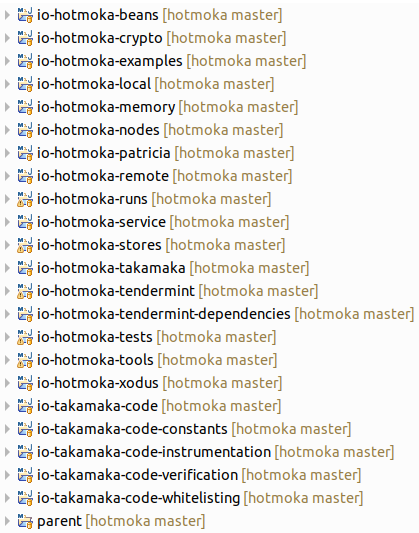
\includegraphics[width=0.6\textwidth,height=\textheight]{pics/projects.png}
\caption{Figure 1. The Eclipse projects of Hotmoka.}
\end{figure}

If you want to see and edit the sources of the Hotmoka project, it is
well possible to import them inside the Eclipse IDE, but this is not
needed for running the examples in the next sections of this tutorial.
For that, use the File → Import → Existing Maven Projects menu item in
Eclipse and import the parent Maven project contained in the
\texttt{hotmoka} directory that you cloned from GitHub. This should
create, inside Eclipse, also its submodule projects. You should see,
inside Eclipse's project explorer, something like Figure 1.

You can compile, package, test and install the Hotmoka jars inside
Eclipse itself, by right-clicking on the \texttt{parent} project and
selecting \texttt{Run\ As} and then the \texttt{Mavel\ install} target.
You can also run the tests inside the Eclipse JUnit runner, by
right-clicking on the \texttt{io-hotmoka-tests} subproject and selecting
\texttt{Run\ As} and then the \texttt{JUnit\ Test} target.

The Maven configuration of the project specifies that all modules and
their dependencies get copied into the \texttt{modules} directory,
classified as automatic, explicit and unnamed modules (as from Java 9
onwards). You can see this by typing:

\begin{myverbatim}
\begin{verbatim}
$ ls -R modules

modules/:
automatic  explicit  unnamed

modules/automatic:
bcel-6.2.jar
spring-beans-5.2.7.RELEASE.jar
spring-core-5.2.7.RELEASE.jar
...
io-hotmoka-tendermint-dependencies-1.0.0.jar
io-hotmoka-xodus-1.0.0.jar
...

modules/explicit:
bcprov-jdk15on-1.67.jar
io-hotmoka-local-1.0.0.jar
io-hotmoka-remote-1.0.0.jar
io-hotmoka-takamaka-1.0.0.jar
io-takamaka-code-constants-1.0.0.jar
it-univr-bcel-1.1.0.jar
gson-2.8.6.jar
io-hotmoka-memory-1.0.0.jar
io-hotmoka-runs-1.0.0.jar
io-hotmoka-tendermint-1.0.0.jar
io-takamaka-code-instrumentation-1.0.0.jar
slf4j-api-1.7.30.jar
io-hotmoka-beans-1.0.0.jar
io-hotmoka-nodes-1.0.0.jar
io-hotmoka-service-1.0.0.jar
io-hotmoka-tools-1.0.0.jar
io-takamaka-code-verification-1.0.0.jar
io-hotmoka-crypto-1.0.0.jar
io-hotmoka-patricia-1.0.0.jar
io-hotmoka-stores-1.0.0.jar
io-takamaka-code-1.0.0.jar
io-takamaka-code-whitelisting-1.0.0.jar

modules/unnamed:
animal-sniffer-annotations-1.18.jar
jakarta.el-3.0.3.jar
...
\end{verbatim}
\end{myverbatim}

It is not possible to discuss here the difference between these kinds of
modules (see \protect\hyperlink{MakB17}{{[}MakB17{]}} for that). Just
remember that explicit and automatic modules must be put in the module
path, while unnamed modules must stay in the class path. Eclipse tries
to do this automatically for us, but often gets confused and you will
have to specify a run configuration sometime. In any case, it is always
possible to run Java from command-line and specify where to put each
category of modules. We will show examples later. For now, let us define
some shell variables that will help us later to put the modules in the
module path or in the class path. Assuming that you are inside the
parent project of Hotmoka, execute:

\begin{myverbatim}
\begin{verbatim}
$ cwd=$(pwd)
$ explicit=$cwd"/modules/explicit"
$ automatic=$cwd"/modules/automatic"
$ unnamed=$cwd"/modules/unnamed"
\end{verbatim}
\end{myverbatim}

or execute the \texttt{set\_variables.sh} shell script, that runs the
same commands:

\begin{myverbatim}
\begin{verbatim}
$ . set_variables.sh
\end{verbatim}
\end{myverbatim}

Variable \texttt{cwd} contains the current directory, where the parent
project of Hotmoka lies. The other three variables contain the directory
of the explicit, automatic and unnamed modules, respectively.

\begin{quote}
The space between the dot and \texttt{set\_variables.sh} guarantees that
the variables remain set after the script terminates.
\end{quote}

The experiments that we will perform in the rest of the tutorial will
require to create Eclipse projects inside a directory that we will name
\texttt{tutorial}. This directory will be a sibling of the
\texttt{hotmoka} repository that you have just cloned. Hence, go out of
the \texttt{hotmoka} repository, create the \texttt{tutorial} directory
and move inside it:

\begin{myverbatim}
\begin{verbatim}
$ cd ..
$ mkdir tutorial
$ cd tutorial
\end{verbatim}
\end{myverbatim}

It is suggested that you experiment with the tutorial examples yourself
and build their projects inside the \texttt{tutorial} directory.
However, if you want to jump to the result directly or if you want to
compare your work with the expected result, there is another repository
that you can clone and that contains the examples of this tutorial, at
each step of development. Each section of this document will report the
project of the repository that you can check out to see the experiments,
as they result after reading that section. Clone the tutorial examples
as a sibling of the \texttt{hotmoka} repository:

\begin{myverbatim}
\begin{verbatim}
$ git clone git@github.com:Hotmoka/hotmoka_tutorial.git
\end{verbatim}
\end{myverbatim}

This will create a \texttt{hotmoka\_tutorial} directory. Inside that
directory, you will find Java Maven projects that show the files at
different steps of this tutorial. For instance, the files at the end of
\protect\hyperlink{creation-eclipse-project}{Creation of the Eclipse
Project}, are inside the project \texttt{family} of the
\texttt{hotmoka\_tutorial} repository. You can import all those projects
into Eclipse (File → Import; then specify \emph{Existing Maven Projects}
and finally select the \texttt{hotmoka\_tutorial} directory).

\hypertarget{a-first-program}{%
\chapter{A First Program }\label{a-first-program}}

Let us start from a simple example of Takamaka code. Since we are
writing Java code, there is nothing special to learn or install before
starting writing programs in Takamaka. Just use your preferred
integrated development environment (IDE) for Java. Or even do everything
from command-line, if you prefer. Our examples below will be shown for
the Eclipse IDE, using Java 11 or later.

Our goal will be to create a Java class that we will instantiate and use
in blockchain. Namely, we will learn how to create an object of the
class that will persist in blockchain and how we can later call the
\texttt{toString()} method on that instance in blockchain.

\hypertarget{creation-of-the-eclipse-project}{%
\section{Creation of the Eclipse Project
}\label{creation-of-the-eclipse-project}}

\textbf{{[}See the \texttt{family} project inside the
\texttt{hotmoka\_tutorial} repository{]}}

Let us create a Maven project \texttt{family} inside Eclipse, in the
\texttt{tutorial} directory. For that, in the Eclipse's Maven wizard
(New → Maven project) specify the options \emph{Create a simple project
(skip archetype selection)} and deselect the \emph{Use default Workspace
directory} option, specifying a subdirectory \texttt{family} of the
\texttt{tutorial} directory as \emph{Location} instead. Hence,
\emph{Location} should be something that ends with
\texttt{.../tutorial/family}. Do not add the project to any working set.
Use \texttt{io.hotmoka} as Group Id and \texttt{family} as Artifact Id.

\begin{quote}
The reason to create the \texttt{tutorial} directory as a sibling of the
\texttt{hotmoka} directory is only to simplify cross-access to the
compiled jar containing the runtime classes of the smart contracts,
without using machine-dependent absolute paths to the local Maven
repository. The Group Id can be changed as you prefer, but we will stick
to \texttt{io.hotmoka} to show the exact files that you will see in
Eclipse.
\end{quote}

By clicking \emph{Finish} in the Eclipse's Maven wizard, you should see
a new Maven project in the Eclipse's explorer. Currently, Eclipse
creates a default \texttt{pom.xml} file that uses Java 5 and has no
dependencies. Replace hence the content of the \texttt{pom.xml} file of
the \texttt{family} project with the code that follows:

\begin{Shaded}
\begin{Highlighting}[]
\KeywordTok{<project}\OtherTok{ xmlns=}\StringTok{"http://maven.apache.org/POM/4.0.0"}
\OtherTok{    xmlns:xsi=}\StringTok{"http://www.w3.org/2001/XMLSchema-instance"}
\OtherTok{    xsi:schemaLocation=}\StringTok{"http://maven.apache.org/POM/4.0.0}
\StringTok{                        http://maven.apache.org/xsd/maven-4.0.0.xsd"}\KeywordTok{>}

  \KeywordTok{<modelVersion>}\NormalTok{4.0.0}\KeywordTok{</modelVersion>}
  \KeywordTok{<groupId>}\NormalTok{io.hotmoka}\KeywordTok{</groupId>}
  \KeywordTok{<artifactId>}\NormalTok{family}\KeywordTok{</artifactId>}
  \KeywordTok{<version>}\NormalTok{0.0.1-SNAPSHOT}\KeywordTok{</version>}

  \KeywordTok{<properties>}
    \KeywordTok{<project.build.sourceEncoding>}\NormalTok{UTF-8}\KeywordTok{</project.build.sourceEncoding>}
    \KeywordTok{<maven.compiler.source>}\NormalTok{11}\KeywordTok{</maven.compiler.source>}
    \KeywordTok{<maven.compiler.target>}\NormalTok{11}\KeywordTok{</maven.compiler.target>}
    \KeywordTok{<failOnMissingWebXml>}\NormalTok{false}\KeywordTok{</failOnMissingWebXml>}
  \KeywordTok{</properties>}

  \KeywordTok{<dependencies>}
    \KeywordTok{<dependency>}
      \KeywordTok{<groupId>}\NormalTok{io.hotmoka}\KeywordTok{</groupId>}
      \KeywordTok{<artifactId>}\NormalTok{io-takamaka-code}\KeywordTok{</artifactId>}
      \KeywordTok{<version>}\NormalTok{1.0.0}\KeywordTok{</version>}
    \KeywordTok{</dependency>}
  \KeywordTok{</dependencies>}

  \KeywordTok{<build>}
    \KeywordTok{<plugins>}
      \KeywordTok{<plugin>}
        \KeywordTok{<groupId>}\NormalTok{org.apache.maven.plugins}\KeywordTok{</groupId>}
        \KeywordTok{<artifactId>}\NormalTok{maven-compiler-plugin}\KeywordTok{</artifactId>}
        \KeywordTok{<version>}\NormalTok{3.8.1}\KeywordTok{</version>}
        \KeywordTok{<configuration>}
          \KeywordTok{<release>}\NormalTok{11}\KeywordTok{</release>}
        \KeywordTok{</configuration>}
      \KeywordTok{</plugin>}
    \KeywordTok{</plugins>}
  \KeywordTok{</build>}

\KeywordTok{</project>}
\end{Highlighting}
\end{Shaded}

that specifies to use Java 11 and provides the dependency that we need,
to the run-time classes of the Takamaka smart contracts.

\begin{quote}
We are using \texttt{1.0.0} here, as version of the Hotmoka and Takamaka
projects. Replace that, if needed, with the current version of such
projects, as printed during their compilation with Maven.
\end{quote}

Since the \texttt{pom.xml} file has changed, Eclipse will normally show
an error on the \texttt{family} project. To solve it, you need to update
the Maven dependencies of the project: right-click on the
\texttt{family} project → Maven → Update Project\ldots{}

As you can see, we are importing the dependency
\texttt{io-takamaka-code}, that contains the Takamaka runtime. If you
have installed the Hotmoka project, this jar has been installed inside
your local Maven repository (as well as in the \texttt{modules/explicit}
directory), hence it is possible to refer to it in the \texttt{pom.xml}
of our project and everything should compile without errors. The result
in Eclipse should look similar to what is shown in Figure 2.

\begin{figure}
\centering
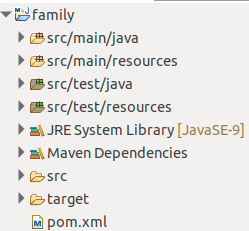
\includegraphics[width=0.4\textwidth,height=\textheight]{pics/family.png}
\caption{Figure 2. The \texttt{family} Eclipse project.}
\end{figure}

Create a \texttt{module-info.java} file inside \texttt{src/main/java}
(right-click on the \texttt{family} project → Configure → Create
module-info.java → Create), to state that this project depends on the
module containing the runtime of Takamaka, needed for development:

\begin{Shaded}
\begin{Highlighting}[]
\NormalTok{module family \{}
\NormalTok{  requires io.}\FunctionTok{takamaka}\NormalTok{.}\FunctionTok{code}\NormalTok{;}
\NormalTok{\}}
\end{Highlighting}
\end{Shaded}

Create a package \texttt{io.takamaka.family} inside
\texttt{src/main/java}. Inside that package, create a Java source
\texttt{Person.java}, by copying and pasting the following code:

\begin{Shaded}
\begin{Highlighting}[]
\KeywordTok{package}\ImportTok{ io.takamaka.family;}

\KeywordTok{public} \KeywordTok{class}\NormalTok{ Person \{}
  \KeywordTok{private} \DataTypeTok{final} \BuiltInTok{String}\NormalTok{ name;}
  \KeywordTok{private} \DataTypeTok{final} \DataTypeTok{int}\NormalTok{ day;}
  \KeywordTok{private} \DataTypeTok{final} \DataTypeTok{int}\NormalTok{ month;}
  \KeywordTok{private} \DataTypeTok{final} \DataTypeTok{int}\NormalTok{ year;}
  \KeywordTok{public} \DataTypeTok{final}\NormalTok{ Person parent1;}
  \KeywordTok{public} \DataTypeTok{final}\NormalTok{ Person parent2;}

  \KeywordTok{public} \FunctionTok{Person}\NormalTok{(}\BuiltInTok{String}\NormalTok{ name, }\DataTypeTok{int}\NormalTok{ day, }\DataTypeTok{int}\NormalTok{ month, }\DataTypeTok{int}\NormalTok{ year,}
\NormalTok{                Person parent1, Person parent2) \{}

    \KeywordTok{this}\NormalTok{.}\FunctionTok{name}\NormalTok{ = name;}
    \KeywordTok{this}\NormalTok{.}\FunctionTok{day}\NormalTok{ = day;}
    \KeywordTok{this}\NormalTok{.}\FunctionTok{month}\NormalTok{ = month;}
    \KeywordTok{this}\NormalTok{.}\FunctionTok{year}\NormalTok{ = year;}
    \KeywordTok{this}\NormalTok{.}\FunctionTok{parent1}\NormalTok{ = parent1;}
    \KeywordTok{this}\NormalTok{.}\FunctionTok{parent2}\NormalTok{ = parent2;}
\NormalTok{  \}}

  \KeywordTok{public} \FunctionTok{Person}\NormalTok{(}\BuiltInTok{String}\NormalTok{ name, }\DataTypeTok{int}\NormalTok{ day, }\DataTypeTok{int}\NormalTok{ month, }\DataTypeTok{int}\NormalTok{ year) \{}
    \KeywordTok{this}\NormalTok{(name, day, month, year, }\KeywordTok{null}\NormalTok{, }\KeywordTok{null}\NormalTok{);}
\NormalTok{  \}}

  \AttributeTok{@Override}
  \KeywordTok{public} \BuiltInTok{String} \FunctionTok{toString}\NormalTok{() \{}
    \KeywordTok{return}\NormalTok{ name + }\StringTok{" ("}\NormalTok{ + day + }\StringTok{"/"}\NormalTok{ + month + }\StringTok{"/"}\NormalTok{ + year + }\StringTok{")"}\NormalTok{;}
\NormalTok{  \}}
\NormalTok{\}}
\end{Highlighting}
\end{Shaded}

This is a plain old Java class and should not need any comment.

Package the project into a jar, by running the following shell command
inside the directory of the project (that is, the subdirectory
\texttt{family} of the directory \texttt{tutorial}):

\begin{myverbatim}
\begin{verbatim}
$ mvn package
\end{verbatim}
\end{myverbatim}

A \texttt{family-0.0.1-SNAPSHOT.jar} file should appear inside the
\texttt{target} directory. Only the compiled class files will be
relevant: Takamaka will ignore source files, manifest and any resources
in the jar; the same compiled \texttt{module-info.class} is irrelevant
for Takamaka. All such files can be removed from the jar, to reduce the
gas cost of their installation in the store of a node, but we do not
care about this optimization here. The result should look as in Figure
3:

\begin{figure}
\centering
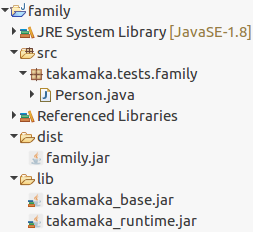
\includegraphics[width=0.4\textwidth,height=\textheight]{pics/family_jar.png}
\caption{Figure 3. The \texttt{family} Eclipse project, exported in
jar.}
\end{figure}

\hypertarget{creation-of-a-hotmoka-node-in-memory}{%
\section{Creation of a Hotmoka Node in Memory
}\label{creation-of-a-hotmoka-node-in-memory}}

\textbf{{[}See the \texttt{blockchain1} project inside the
\texttt{hotmoka\_tutorial} repository{]}}

The next step is to install in blockchain the jar of the \texttt{family}
project, use it to create an instance of \texttt{Person} and call
\texttt{toString()} on that instance. For that, we need a local
blockchain consisting of a single node.

\begin{quote}
We will perform this process first with a simulation of a blockchain,
whose use is simpler and faster, and subsequently with a real
blockchain.
\end{quote}

Let us hence create another Eclipse Maven project \texttt{blockchain},
inside \texttt{tutorial}, exactly as we did in the previous section for
the \texttt{family} project. We will specify Java 11 (or later) in its
build path. This project will start a local simulation of a blockchain
node, actually working over the disk memory of our local machine. Hence
this project depends on the jar that implements that blockchain
simulation in memory. The latter simulation is an example of a Hotmoka
node. Use \texttt{io.hotmoka} as Group Id and \texttt{blockchain} as
Artifact Id. This is specified in the following \texttt{pom.xml}, that
we will copy inside the \texttt{blockchain} project, replacing that
generated by Eclipse:

\begin{Shaded}
\begin{Highlighting}[]
\KeywordTok{<project}\OtherTok{ xmlns=}\StringTok{"http://maven.apache.org/POM/4.0.0"}
\OtherTok{  xmlns:xsi=}\StringTok{"http://www.w3.org/2001/XMLSchema-instance"}
\OtherTok{  xsi:schemaLocation=}\StringTok{"http://maven.apache.org/POM/4.0.0}
\StringTok{                      http://maven.apache.org/xsd/maven-4.0.0.xsd"}\KeywordTok{>}

  \KeywordTok{<modelVersion>}\NormalTok{4.0.0}\KeywordTok{</modelVersion>}

  \KeywordTok{<groupId>}\NormalTok{io.hotmoka}\KeywordTok{</groupId>}
  \KeywordTok{<artifactId>}\NormalTok{blockchain}\KeywordTok{</artifactId>}
  \KeywordTok{<version>}\NormalTok{0.0.1-SNAPSHOT}\KeywordTok{</version>}
  \KeywordTok{<packaging>}\NormalTok{jar}\KeywordTok{</packaging>}

  \KeywordTok{<properties>}
    \KeywordTok{<project.build.sourceEncoding>}\NormalTok{UTF-8}\KeywordTok{</project.build.sourceEncoding>}
    \KeywordTok{<maven.compiler.source>}\NormalTok{11}\KeywordTok{</maven.compiler.source>}
    \KeywordTok{<maven.compiler.target>}\NormalTok{11}\KeywordTok{</maven.compiler.target>}
    \KeywordTok{<failOnMissingWebXml>}\NormalTok{false}\KeywordTok{</failOnMissingWebXml>}
  \KeywordTok{</properties>}

  \KeywordTok{<build>}
    \KeywordTok{<plugins>}
      \KeywordTok{<plugin>}
        \KeywordTok{<groupId>}\NormalTok{org.apache.maven.plugins}\KeywordTok{</groupId>}
        \KeywordTok{<artifactId>}\NormalTok{maven-compiler-plugin}\KeywordTok{</artifactId>}
        \KeywordTok{<version>}\NormalTok{3.8.1}\KeywordTok{</version>}
        \KeywordTok{<configuration>}
          \KeywordTok{<release>}\NormalTok{11}\KeywordTok{</release>}
        \KeywordTok{</configuration>}
      \KeywordTok{</plugin>}
    \KeywordTok{</plugins>}
  \KeywordTok{</build>}

  \KeywordTok{<dependencies>}
    \KeywordTok{<dependency>}
      \KeywordTok{<groupId>}\NormalTok{io.hotmoka}\KeywordTok{</groupId>}
      \KeywordTok{<artifactId>}\NormalTok{io-hotmoka-memory}\KeywordTok{</artifactId>}
      \KeywordTok{<version>}\NormalTok{1.0.0}\KeywordTok{</version>}
    \KeywordTok{</dependency>}
  \KeywordTok{</dependencies>}

\KeywordTok{</project>}
\end{Highlighting}
\end{Shaded}

It specifies as dependency the \texttt{io-hotmoka-memory} module, that
contains a Hotmoka node that implements a disk memory simulation of a
blockchain. It has been installed in our local Maven repository
previously, when we packaged and installed the Hotmoka project.

Since we modified the file \texttt{pom.xml}, Eclipse should show an
error for the \texttt{blockchain} project. To fix it, you need to update
the Maven dependencies of the project: right-click on the
\texttt{blockchain} project → Maven → Update Project\ldots{}

Leave directory \texttt{src/test/java} empty, by deleting its content,
if not already empty.

The result should look like as in Figure 4.

\begin{figure}
\centering
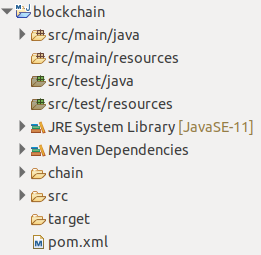
\includegraphics[width=0.4\textwidth,height=\textheight]{pics/blockchain1.png}
\caption{Figure 4. The \texttt{blockchain} Eclipse project.}
\end{figure}

Create a \texttt{module-info.java} inside \texttt{src/main/java},
containing:

\begin{Shaded}
\begin{Highlighting}[]
\NormalTok{module blockchain \{}
\NormalTok{  requires io.}\FunctionTok{hotmoka}\NormalTok{.}\FunctionTok{memory}\NormalTok{;}
\NormalTok{  requires io.}\FunctionTok{hotmoka}\NormalTok{.}\FunctionTok{beans}\NormalTok{;}
\NormalTok{  requires io.}\FunctionTok{hotmoka}\NormalTok{.}\FunctionTok{nodes}\NormalTok{;}
\NormalTok{\}}
\end{Highlighting}
\end{Shaded}

Create a package \texttt{io.takamaka.family} inside
\texttt{src/main/java} and add the following class \texttt{Main.java}
inside it:

\begin{Shaded}
\begin{Highlighting}[]
\KeywordTok{package}\ImportTok{ io.takamaka.family;}

\KeywordTok{import}\ImportTok{ io.hotmoka.memory.MemoryBlockchain;}
\KeywordTok{import}\ImportTok{ io.hotmoka.memory.MemoryBlockchainConfig;}
\KeywordTok{import}\ImportTok{ io.hotmoka.nodes.ConsensusParams;}
\KeywordTok{import}\ImportTok{ io.hotmoka.nodes.Node;}

\KeywordTok{public} \KeywordTok{class}\NormalTok{ Main \{}

  \KeywordTok{public} \DataTypeTok{static} \DataTypeTok{void} \FunctionTok{main}\NormalTok{(}\BuiltInTok{String}\NormalTok{[] args) }\KeywordTok{throws} \BuiltInTok{Exception}\NormalTok{ \{}
\NormalTok{    MemoryBlockchainConfig config = }\KeywordTok{new}\NormalTok{ MemoryBlockchainConfig.}\FunctionTok{Builder}\NormalTok{().}\FunctionTok{build}\NormalTok{();}
\NormalTok{    ConsensusParams consensus = }\KeywordTok{new}\NormalTok{ ConsensusParams.}\FunctionTok{Builder}\NormalTok{().}\FunctionTok{build}\NormalTok{();}

    \KeywordTok{try}\NormalTok{ (}\BuiltInTok{Node}\NormalTok{ node = MemoryBlockchain.}\FunctionTok{init}\NormalTok{(config, consensus)) \{}
      \CommentTok{// the node is closed automatically at the end of this block}
\NormalTok{    \}}
\NormalTok{  \}}
\NormalTok{\}}
\end{Highlighting}
\end{Shaded}

As you can see, this class simply creates an instance of the blockchain
on disk memory. The blockchain is an \texttt{AutoCloseable} Hotmoka
node, hence it is placed inside a try with resource that guarantees its
release at the end of the \texttt{try} block. The \texttt{config}
parameter allows us to provide some initialization options to the node
of the blockchain. The \texttt{consensus} parameter allows us to specify
the consensus parameters of the network the node belongs to. We have
used its default values for both here.

Like every Hotmoka node, the observable state of the blockchain can only
evolve through \emph{transactions}, that modify its state in an atomic
way.

An important point is that this blockchain is completely empty after
creation. It does not contain data, but it does not contain code either.
It is not even possible to invoke static methods of the standard Java
library, since the invocation of code in a Hotmoka node requires to
identify an object, the \emph{caller}, ie. an instance of
\texttt{io.takamaka.code.lang.ExternallyOwnedAccount} that pays for the
execution of the transaction that runs the code. But also that class is
not installed in the store of the node yet. Hence, we cannot actually
run any transaction on this brand new node. To solve this problem,
Hotmoka nodes can execute \emph{initial} transactions that do not
require any caller. In that sense, they are executed \emph{for free}.
Thus, what we need is to run a sequence of initial transactions that
perform the following tasks:

\begin{enumerate}
\def\labelenumi{\arabic{enumi}.}
\tightlist
\item
  install \texttt{io.takamaka.code-1.0.0.jar} inside the store of the
  node. That jar contains the
  \texttt{io.takamaka.code.lang.ExternallyOwnedAccount} class and many
  other classes that we can use for programming our smart contracts.
  They form the runtime of Takamaka;
\item
  choose a pair of private and public keys and create, in the store of
  the node, an object of class
  \texttt{io.takamaka.code.lang.ExternallyOwnedAccount}, controlled by
  those keys, that holds all money initially provided to the node. This
  object is called \emph{gamete} and can be used later to fund other
  accounts;
\item
  create an object of class
  \texttt{io.takamaka.code.governance.Validators}, that describes the
  nodes that are in charge of validating the transactions of the node
  (currently, this will be empty);
\item
  create an object of class
  \texttt{io.takamaka.code.governance.Manifest}, that is used to publish
  information about the node. For instance, it tells who is the gamete
  of the node and which is the chain identifier of the node, and gives
  access to the container of validators created at point 3 above;
\item
  state that the node has been initialized. After this statement, no
  more initial transactions can be run with this node (they would be
  rejected).
\end{enumerate}

It is interesting to know how this initialization process works, but
users of a Hotmoka node are very unlikely interested in these details.
Hence, we do not discuss it further and, instead, use a node decorator
that performs, for us, the above transactions, effectively initializing
a node that needs initialization:

\begin{Shaded}
\begin{Highlighting}[]
\KeywordTok{package}\ImportTok{ io.takamaka.family;}

\KeywordTok{import}\ImportTok{ java.math.BigInteger;}
\KeywordTok{import}\ImportTok{ java.nio.file.Path;}
\KeywordTok{import}\ImportTok{ java.nio.file.Paths;}

\KeywordTok{import}\ImportTok{ io.hotmoka.memory.MemoryBlockchain;}
\KeywordTok{import}\ImportTok{ io.hotmoka.memory.MemoryBlockchainConfig;}
\KeywordTok{import}\ImportTok{ io.hotmoka.nodes.ConsensusParams;}
\KeywordTok{import}\ImportTok{ io.hotmoka.nodes.Node;}
\KeywordTok{import}\ImportTok{ io.hotmoka.nodes.views.InitializedNode;}

\KeywordTok{public} \KeywordTok{class}\NormalTok{ Main \{}
  \KeywordTok{public} \DataTypeTok{final} \DataTypeTok{static} \BuiltInTok{BigInteger}\NormalTok{ GREEN_AMOUNT = }\BuiltInTok{BigInteger}\NormalTok{.}\FunctionTok{valueOf}\NormalTok{(}\DecValTok{100_000_000}\NormalTok{);}
  \KeywordTok{public} \DataTypeTok{final} \DataTypeTok{static} \BuiltInTok{BigInteger}\NormalTok{ RED_AMOUNT = }\BuiltInTok{BigInteger}\NormalTok{.}\FunctionTok{ZERO}\NormalTok{;}

  \KeywordTok{public} \DataTypeTok{static} \DataTypeTok{void} \FunctionTok{main}\NormalTok{(}\BuiltInTok{String}\NormalTok{[] args) }\KeywordTok{throws} \BuiltInTok{Exception}\NormalTok{ \{}
\NormalTok{    MemoryBlockchainConfig config = }\KeywordTok{new}\NormalTok{ MemoryBlockchainConfig.}\FunctionTok{Builder}\NormalTok{().}\FunctionTok{build}\NormalTok{();}
\NormalTok{    ConsensusParams consensus = }\KeywordTok{new}\NormalTok{ ConsensusParams.}\FunctionTok{Builder}\NormalTok{().}\FunctionTok{build}\NormalTok{();}

    \CommentTok{// the path of the packaged runtime Takamaka classes}
\NormalTok{    Path takamakaCodePath = Paths.}\FunctionTok{get}
\NormalTok{      (}\StringTok{"../../hotmoka/modules/explicit/io-takamaka-code-1.0.0.jar"}\NormalTok{);}

    \KeywordTok{try}\NormalTok{ (}\BuiltInTok{Node}\NormalTok{ node = MemoryBlockchain.}\FunctionTok{init}\NormalTok{(config, consensus)) \{}
\NormalTok{      InitializedNode initialized = InitializedNode.}\FunctionTok{of}
\NormalTok{        (node, consensus, takamakaCodePath, GREEN_AMOUNT, RED_AMOUNT);}
\NormalTok{    \}}
\NormalTok{  \}}
\NormalTok{\}}
\end{Highlighting}
\end{Shaded}

The code above initializes the node, performing steps 1-5 above. It
installs the runtime of Takamaka, that we had previously packaged inside
the project \texttt{io-takamaka-code} (the relative path works since we
put \texttt{tutorial} as a sibling of the \texttt{hotmoka} directory).
It sets the empty string as its chain identifier.

\begin{quote}
The chain identifier is used to avoid replaying of transactions across
distinct networks. That is, a transaction sent to a network must specify
the same chain identifier reported in the manifest of the nodes of the
network, or otherwise it will be rejected.
\end{quote}

It is important to observe that both \texttt{node} and
\texttt{initialized} are views of the same Hotmoka node. Hence, if we
run \texttt{Main}, both get initialized and both will contain the
\texttt{io-takamaka-code-1.0.0.jar} archive and a new object, the
gamete, initialized with the given amounts of green and red coins.

Package the \texttt{blockchain} project and run it (the \texttt{java}
invocation command is on a single line):

\begin{myverbatim}
\begin{verbatim}
$ cd blockchain
$ mvn package
$ java --module-path $explicit:$automatic:target/blockchain-0.0.1-SNAPSHOT.jar
       -classpath $unnamed"/*"
       --module blockchain/io.takamaka.family.Main
\end{verbatim}
\end{myverbatim}

\begin{quote}
In the following, when we say to run a \texttt{main()} method of a class
of the \texttt{blockchain} project, we mean to use a \texttt{java}
invocation as the one given above. You can also right-click on the
\texttt{Main.java} file in Eclipse and select Run as → Java Application.
As another alternative, you can create a run configuration in Eclipse
and edit its dependencies in such a way to add all explicit and
automatic modules in its module path and all unnamed modules in its
class path.
\end{quote}

Refresh the \texttt{blockchain} project in Eclipse now (click on it and
push the F5 key). You will see that a new directory \texttt{chain}
appeared, that contains blocks such as \texttt{b0} and \texttt{b1}.
Inside these blocks, there are transactions, implementing the five steps
above, that initialize a Hotmoka node (see Figure 5).

\begin{figure}
\centering
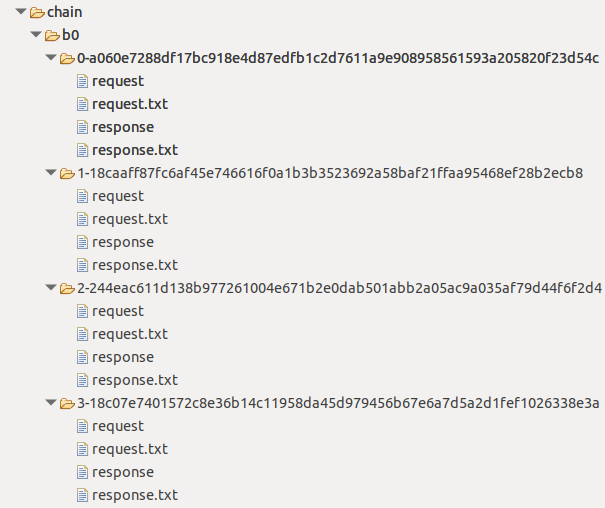
\includegraphics[width=0.9\textwidth,height=\textheight]{pics/blockchain2.png}
\caption{Figure 5. The \texttt{chain} directory appeared.}
\end{figure}

Each transaction is specified by a request and a corresponding response.
They are kept in serialized form (\texttt{request} and
\texttt{response}) but are also reported in textual form
(\texttt{request.txt} and \texttt{response.txt}). Such textual
representations do not exist in a real blockchain, but are useful here,
for debugging and for learning. We do not investigate further the
content of the \texttt{chain} directory, for now. Later, when we will
run our own transactions, we will see these files in more detail.

\hypertarget{a-transaction-that-stores-a-jar-in-a-hotmoka-node}{%
\section{A Transaction that Stores a Jar in a Hotmoka Node
}\label{a-transaction-that-stores-a-jar-in-a-hotmoka-node}}

\textbf{{[}See project \texttt{blockchain2} inside the
\texttt{hotmoka\_tutorial} repository{]}}

The previous section has shown how to create a brand new blockchain and
initialize it with the runtime of Takamaka and a gamete. Our original
goal was to use that blockchain to store an instance of the
\texttt{Person} class. That class is not in the build path of the
\texttt{blockchain} project, nor in its class or module path at run
time. If we want to call the constructor of \texttt{Person}, that class
must somehow be accessible. In order to make \texttt{Person} accessible,
we must run a transaction that installs
\texttt{family-0.0.1-SNAPSHOT.jar} inside the blockchain, so that we can
later refer to it and call the constructor of \texttt{Person}. This will
not be an initial transaction (the node has been already definitely
initialized). Hence, it must be paid by an externally owned account. The
only such account that is available by now is the gamete that has been
created during initialization.

Let us hence use that gamete as caller of a transaction that stores
\texttt{family-0.0.1-SNAPSHOT.jar} in blockchain. This seems like a very
easy task, but actually hides many smaller problems. We have said that
the gamete must pay for that transaction. Then it must sign the
transaction request with its private key. Where are the gamete and the
key? It turns out that the \texttt{InitializedNode} view has a
\texttt{gamete()} method that yields the storage reference of the gamete
and a \texttt{keysOfGamete()} method that allows one to read the keys of
the gamete. Note that its private key is not in blockchain, but only in
the view, that is a Java object in RAM. There is a last problem to solve
before we can put everything in place. Transaction requests include a
nonce, to avoid replaying of transactions and to ensure that they are
executed in the right order. Hence the request to install a new jar in
blockchain must specify the nonce of the caller, that is, the nonce of
the gamete. In order to get that nonce, we can call the \texttt{nonce()}
method of the gamete. But which account do we use as caller of this
other transaction? It turns out that we can use the gamete
itself\ldots{} this is possible since the \texttt{nonce()} method is
declared as \texttt{@View}. We will see later what this means. For now,
it is relevant to know that calls to \texttt{@View} methods can be run
with \emph{any} nonce, since it will not be used nor checked. Let us
just use zero for that nonce then.

A final consideration is related to gas. As in Ethereum, transactions
are paid in terms of gas consumed for their execution. In the following,
we will use zero as gas price when running calls to \texttt{@View}
methods. This is because such calls do not actually modify the state of
the node and are executed locally, on the node that receives the request
of the transaction. Hence, they can be considered as run \emph{for
free}. Instead, we will use an actual gas price for the last transaction
that installs the jar in blockchain. This could be computed with a
sequence of cllas to \texttt{@View} methods (get the manifest, them the
gas station inside the manifest, then the gas price inside the gas
station). In order to simplify the code, we will use the
\texttt{GasHelper} class, that does exactly that for us.

The result is the following code. It first initializes a new blockchain
and then installs the archive \texttt{family-0.0.1-SNAPSHOT.jar} in it:

\begin{Shaded}
\begin{Highlighting}[]
\KeywordTok{package}\ImportTok{ io.takamaka.family;}

\KeywordTok{import static}\ImportTok{ java.math.BigInteger.ONE;}
\KeywordTok{import static}\ImportTok{ java.math.BigInteger.ZERO;}

\KeywordTok{import}\ImportTok{ java.math.BigInteger;}
\KeywordTok{import}\ImportTok{ java.nio.file.Files;}
\KeywordTok{import}\ImportTok{ java.nio.file.Path;}
\KeywordTok{import}\ImportTok{ java.nio.file.Paths;}

\KeywordTok{import}\ImportTok{ io.hotmoka.beans.references.TransactionReference;}
\KeywordTok{import}\ImportTok{ io.hotmoka.beans.requests.InstanceMethodCallTransactionRequest;}
\KeywordTok{import}\ImportTok{ io.hotmoka.beans.requests.JarStoreTransactionRequest;}
\KeywordTok{import}\ImportTok{ io.hotmoka.beans.requests.SignedTransactionRequest;}
\KeywordTok{import}\ImportTok{ io.hotmoka.beans.requests.SignedTransactionRequest.Signer;}
\KeywordTok{import}\ImportTok{ io.hotmoka.beans.signatures.NonVoidMethodSignature;}
\KeywordTok{import}\ImportTok{ io.hotmoka.beans.types.ClassType;}
\KeywordTok{import}\ImportTok{ io.hotmoka.beans.values.BigIntegerValue;}
\KeywordTok{import}\ImportTok{ io.hotmoka.beans.values.StorageReference;}
\KeywordTok{import}\ImportTok{ io.hotmoka.crypto.SignatureAlgorithm;}
\KeywordTok{import}\ImportTok{ io.hotmoka.memory.MemoryBlockchain;}
\KeywordTok{import}\ImportTok{ io.hotmoka.memory.MemoryBlockchainConfig;}
\KeywordTok{import}\ImportTok{ io.hotmoka.nodes.ConsensusParams;}
\KeywordTok{import}\ImportTok{ io.hotmoka.nodes.GasHelper;}
\KeywordTok{import}\ImportTok{ io.hotmoka.nodes.Node;}
\KeywordTok{import}\ImportTok{ io.hotmoka.nodes.views.InitializedNode;}

\KeywordTok{public} \KeywordTok{class}\NormalTok{ Main \{}
  \KeywordTok{public} \DataTypeTok{final} \DataTypeTok{static} \BuiltInTok{BigInteger}\NormalTok{ GREEN_AMOUNT = }\BuiltInTok{BigInteger}\NormalTok{.}\FunctionTok{valueOf}\NormalTok{(}\DecValTok{100_000_000}\NormalTok{);}
  \KeywordTok{public} \DataTypeTok{final} \DataTypeTok{static} \BuiltInTok{BigInteger}\NormalTok{ RED_AMOUNT = }\BuiltInTok{BigInteger}\NormalTok{.}\FunctionTok{ZERO}\NormalTok{;}

  \KeywordTok{public} \DataTypeTok{static} \DataTypeTok{void} \FunctionTok{main}\NormalTok{(}\BuiltInTok{String}\NormalTok{[] args) }\KeywordTok{throws} \BuiltInTok{Exception}\NormalTok{ \{}
\NormalTok{    MemoryBlockchainConfig config = }\KeywordTok{new}\NormalTok{ MemoryBlockchainConfig.}\FunctionTok{Builder}\NormalTok{().}\FunctionTok{build}\NormalTok{();}
\NormalTok{    ConsensusParams consensus = }\KeywordTok{new}\NormalTok{ ConsensusParams.}\FunctionTok{Builder}\NormalTok{().}\FunctionTok{build}\NormalTok{();}

    \CommentTok{// the path of the packaged runtime Takamaka classes}
\NormalTok{    Path takamakaCodePath = Paths.}\FunctionTok{get}
\NormalTok{      (}\StringTok{"../../hotmoka/modules/explicit/io-takamaka-code-1.0.0.jar"}\NormalTok{);}

    \CommentTok{// the path of the user jar to install}
\NormalTok{    Path familyPath = Paths.}\FunctionTok{get}\NormalTok{(}\StringTok{"../family/target/family-0.0.1-SNAPSHOT.jar"}\NormalTok{);}

    \KeywordTok{try}\NormalTok{ (}\BuiltInTok{Node}\NormalTok{ node = MemoryBlockchain.}\FunctionTok{init}\NormalTok{(config, consensus)) \{}
      \CommentTok{// we store io-takamaka-code-1.0.0.jar and create the manifest and the gamete}
\NormalTok{      InitializedNode initialized = InitializedNode.}\FunctionTok{of}
\NormalTok{        (node, consensus, takamakaCodePath, GREEN_AMOUNT, RED_AMOUNT);}

      \CommentTok{// we get a reference to where io-takamaka-code-1.0.0.jar has been stored}
\NormalTok{      TransactionReference takamakaCode = node.}\FunctionTok{getTakamakaCode}\NormalTok{();}

      \CommentTok{// we get a reference to the gamete}
\NormalTok{      StorageReference gamete = initialized.}\FunctionTok{gamete}\NormalTok{();}

      \CommentTok{// we get the signing algorithm to use for requests}
\NormalTok{      SignatureAlgorithm<SignedTransactionRequest> signature}
\NormalTok{        = node.}\FunctionTok{getSignatureAlgorithmForRequests}\NormalTok{();}

      \CommentTok{// we create a signer that signs with the private key of the gamete}
      \BuiltInTok{Signer}\NormalTok{ signerOnBehalfOfGamete = }\BuiltInTok{Signer}\NormalTok{.}\FunctionTok{with}
\NormalTok{        (signature, initialized.}\FunctionTok{keysOfGamete}\NormalTok{().}\FunctionTok{getPrivate}\NormalTok{());}

      \CommentTok{// we get the nonce of the gamete: we use the gamete as caller and}
      \CommentTok{// an arbitrary nonce (ZERO in the code) since we are running}
      \CommentTok{// a @View method of the gamete}
      \BuiltInTok{BigInteger}\NormalTok{ nonce = ((BigIntegerValue) node}
\NormalTok{        .}\FunctionTok{runInstanceMethodCallTransaction}\NormalTok{(}\KeywordTok{new}\NormalTok{ InstanceMethodCallTransactionRequest}
\NormalTok{          (signerOnBehalfOfGamete, }\CommentTok{// an object that signs with the payer's private key}
\NormalTok{          gamete, }\CommentTok{// payer}
\NormalTok{          ZERO, }\CommentTok{// nonce: irrelevant for calls to a @View method}
          \StringTok{""}\NormalTok{, }\CommentTok{// chain identifier: irrelevant for calls to a @View method}
          \BuiltInTok{BigInteger}\NormalTok{.}\FunctionTok{valueOf}\NormalTok{(}\DecValTok{10_000}\NormalTok{), }\CommentTok{// gas limit}
\NormalTok{          ZERO, }\CommentTok{// gas price: irrelevant for calls to a @View method}
\NormalTok{          takamakaCode, }\CommentTok{// class path for the execution of the transaction}

          \CommentTok{// method}
          \KeywordTok{new}\NormalTok{ NonVoidMethodSignature}
\NormalTok{            (}\StringTok{"io.takamaka.code.lang.Account"}\NormalTok{, }\StringTok{"nonce"}\NormalTok{, ClassType.}\FunctionTok{BIG_INTEGER}\NormalTok{),}

\NormalTok{          gamete))) }\CommentTok{// receiver of the method call}
\NormalTok{        .}\FunctionTok{value}\NormalTok{;}

\NormalTok{      GasHelper gasHelper = }\KeywordTok{new} \FunctionTok{GasHelper}\NormalTok{(node);}

      \CommentTok{// we install family-0.0.1-SNAPSHOT.jar in blockchain: the gamete will pay}
\NormalTok{      TransactionReference family = node}
\NormalTok{        .}\FunctionTok{addJarStoreTransaction}\NormalTok{(}\KeywordTok{new}\NormalTok{ JarStoreTransactionRequest}
\NormalTok{          (signerOnBehalfOfGamete, }\CommentTok{// an object that signs with the payer's private key}
\NormalTok{          gamete, }\CommentTok{// payer}
\NormalTok{          nonce, }\CommentTok{// payer's nonce: relevant since this is not a call to a @View method!}
          \StringTok{""}\NormalTok{, }\CommentTok{// chain identifier: relevant since this is not a call to a @View method!}
          \BuiltInTok{BigInteger}\NormalTok{.}\FunctionTok{valueOf}\NormalTok{(}\DecValTok{10_000}\NormalTok{), }\CommentTok{// gas limit: enough for this very small jar}
\NormalTok{          gasHelper.}\FunctionTok{getSafeGasPrice}\NormalTok{(), }\CommentTok{// gas price: at least the current gas price}
\NormalTok{          takamakaCode, }\CommentTok{// class path for the execution of the transaction}
\NormalTok{          Files.}\FunctionTok{readAllBytes}\NormalTok{(familyPath), }\CommentTok{// bytes of the jar to install}
\NormalTok{          takamakaCode)); }\CommentTok{// dependencies of the jar that is being installed}

      \BuiltInTok{System}\NormalTok{.}\FunctionTok{out}\NormalTok{.}\FunctionTok{println}\NormalTok{(}\StringTok{"manifest: "}\NormalTok{ + node.}\FunctionTok{getManifest}\NormalTok{());}
      \BuiltInTok{System}\NormalTok{.}\FunctionTok{out}\NormalTok{.}\FunctionTok{println}\NormalTok{(}\StringTok{"gamete: "}\NormalTok{ + gamete);}
      \BuiltInTok{System}\NormalTok{.}\FunctionTok{out}\NormalTok{.}\FunctionTok{println}\NormalTok{(}\StringTok{"nonce of gamete: "}\NormalTok{ + nonce);}
      \BuiltInTok{System}\NormalTok{.}\FunctionTok{out}\NormalTok{.}\FunctionTok{println}\NormalTok{(}\StringTok{"family-0.0.1-SNAPSHOT.jar: "}\NormalTok{ + family);}

      \CommentTok{// we increase to nonce, ready for further transactions having the gamete as payer}
\NormalTok{      nonce = nonce.}\FunctionTok{add}\NormalTok{(ONE);}
\NormalTok{    \}}
\NormalTok{  \}}
\NormalTok{\}}
\end{Highlighting}
\end{Shaded}

Package the \texttt{blockchain} project and run this class, as explained
in the previous section. Its execution should print something like this
on the screen:

\begin{myverbatim}
\begin{verbatim}
manifest: 7d86cb8b8fc905bd7ea4cde5d1003f495e521b25ed3e864ce7c2d41cf67bf524#0
gamete: c943faf51f9567d7fa2d76770132a633e7e1b771d9f5cb0473e44dc131388385#0
nonce of gamete: 3
family-0.0.1-SNAPSHOT.jar: 4c5977f8f621cfeca03b903ab3a69b2cbf1ea76ca1138a312900ad...
\end{verbatim}
\end{myverbatim}

\begin{quote}
Different runs will print different values, since the key pair of the
gamete will vary randomly.
\end{quote}

The \texttt{addJarStoreTransaction()} method executes a new transaction
on the node, whose goal is to install a jar inside it. The jar is
provided as a sequence of bytes
(\texttt{Files.readAllBytes(Paths.get("../family/target/family-0.0.1-SNAPSHOT.jar"))},
assuming that the \texttt{family} project is a sibling of the project
\texttt{blockchain}). This transaction, as all non-initial transactions,
must be paid. We use the \texttt{gamete} as payer. We compute its
\texttt{nonce} with a call to method
\texttt{runInstanceMethodCallTransaction()} on the \texttt{gamete}
object. The request passed to \texttt{addJarStoreTransaction()}
specifies that the transaction can cost up to 10,000 units of gas, that
can be bought at a price returned by the \texttt{gasHelper} object. The
request specifies that its class path is
\texttt{node.getTakamakaCode()}: this is the reference to the
\texttt{io-takamaka-code-1.0.0.jar} installed by the
\texttt{InitializedNode} decorator. Finally, the request specifies that
\texttt{family-0.0.1-SNAPSHOT.jar} has only a single dependency:
\texttt{io-takamaka-code-1.0.0.jar}. This means that when, below, we
will refer to \texttt{family-0.0.1-SNAPSHOT.jar} in a class path, this
will indirectly include its dependency
\texttt{io-takamaka-code-1.0.0.jar} as well.

Refresh the parent project and see how the \texttt{chain} directory is
one transaction longer now (see Figure 6).

\begin{figure}
\centering
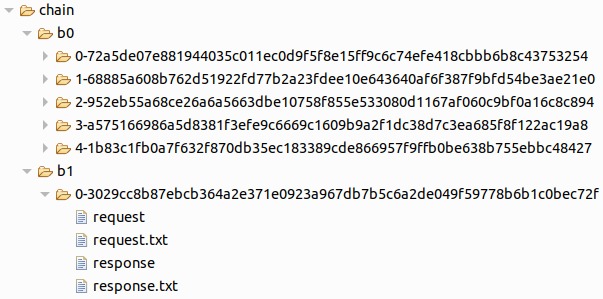
\includegraphics[width=0.9\textwidth,height=\textheight]{pics/blockchain3.png}
\caption{Figure 6. A new transaction appeared in the \texttt{chain}
directory.}
\end{figure}

The new transaction reports a \texttt{request} that corresponds to the
request that we have coded in the \texttt{Main} class. Namely, its
textual representation \texttt{request.txt} is:

\begin{myverbatim}
\begin{verbatim}
JarStoreTransactionRequest:
  caller: 9af31c9fb995cf1a32b3589b2df29276a4388f3207560896e5f971a86aec1eba#0
  nonce: 3
  gas limit: 10000
  gas price: 200
  class path: 0e13b558c03ededf19319a5b1b42b0efb1cf820316016893c01cc4b0ed48a6d1
  chainId: 
  dependencies: [0e13b558c03ededf19319a5b1b42b0efb1cf820316016893c01cc4b0ed48a6d1]
  jar: 504b03040a0000000000a4885a52000000000000000000000000090000004d4554412d49...
  signature: 7fc3f2bb770de510915d351b71b98116659b4119dfb4ee636ee76183e8b8aba9d1...
\end{verbatim}
\end{myverbatim}

Note that objects, such as the caller account \texttt{gamete}, are
represented here as \emph{storage references} such as
\texttt{9af31c9fb995cf1a32b3589b2df29276a4388f3207560896e5f971a86aec1eba\#0}.
You can think at a storage reference as a machine-independent,
deterministic pointer to an object in the store of the node. Also the
dependency \texttt{io-takamaka-code-1.0.0.jar} is represented as a
\emph{transaction reference}
\texttt{0e13b558c03ededf19319a5b1b42b0efb1cf820316016893c01cc4b0ed48a6d1},
that is, a reference to the transaction that installed
\texttt{io-takamaka-code-1.0.0.jar} in the node. Note that, in this
case, it coincides with the class path of the transaction. The jar in
the request is the hexadecimal representation of its byte sequence.

Let us have a look at the \texttt{response.txt} file, that is the
textual representation of the outcome of the transaction:

\begin{myverbatim}
\begin{verbatim}
JarStoreTransactionSuccessfulResponse:
  gas consumed for CPU execution: 259
  gas consumed for RAM allocation: 1286
  gas consumed for storage consumption: 1647
  updates:
    <9af31c9fb995cf1a32b3589b2df29276a4388f3207560896e5f971a86aec1eba#0|
      io.takamaka.code.lang.Contract.balance:java.math.BigInteger
      |99361600>
    <9af31c9fb995cf1a32b3589b2df29276a4388f3207560896e5f971a86aec1eba#0|
      io.takamaka.code.lang.RedGreenExternallyOwnedAccount.nonce
      :java.math.BigInteger|4>
  instrumented jar: 504b0304140008080800000021000000000000000000000000001f00...
\end{verbatim}
\end{myverbatim}

The first bits of information tell us that the transaction costed some
units of gas, split between CPU, RAM and node storage space. We had
accepted to spend up to 10,000 units of gas, hence the transaction could
complete correctly. The response reports also the hexadecimal
representation of a jar, qualified as \emph{instrumented}. This is
because what gets installed in the store of the node is not exactly the
jar sent with the transaction request, but an instrumentation of that,
that adds features specific to Takamaka code. For instance, the
instrumented code will charge gas during its execution. Finally, the
response reports \emph{updates}. These are state changes occurred during
the execution of the transaction. In other terms, updates are the
side-effects of the transaction, ie., the fields of the objects modified
by the transaction. In this case, the balance of the gamete has been
reduced to 99,361,600, since it paid for the gas (we have initially
funded that gamete with 100,000,000 units of coin) and its nonce has
been incremented to 4, since the gamete has been used to run another
transaction.

\begin{quote}
The actual amount of gas consumed by this transaction, the bytes of the
jars and the final balance of the payer might change in different
versions of Takamaka.
\end{quote}

Before concluding this section, note that the call to
\texttt{runInstanceMethodCallTransaction()} has not generated any entry
among the transactions recorded in the \texttt{chain} folder. As we said
before, that method runs \texttt{@View} methods, that induce no updates
and that can hence be executed by a single node, without need of
consensus with the other nodes. The advantage is that we do not pay for
those transactions and do not need to compute a correct nonce for them.
Such requests do not need a chain identifier and do not need to be
signed. The drawback is that their transactions are not checked by
consensus, hence we have to trust the node we ask. Moreover, they can
only read, never write the data in the store of the node. Since method
\texttt{runInstanceMethodCallTransaction()} does not need all fields of
the request to be filled, there is a simpler constructor for the request
that can be used here. Namely, the code that computes the nonce can be
simplified into:

\begin{Shaded}
\begin{Highlighting}[]
\BuiltInTok{BigInteger}\NormalTok{ nonce = ((BigIntegerValue) node}
\NormalTok{  .}\FunctionTok{runInstanceMethodCallTransaction}\NormalTok{(}\KeywordTok{new}\NormalTok{ InstanceMethodCallTransactionRequest}
\NormalTok{    (gamete, }\CommentTok{// payer}
     \BuiltInTok{BigInteger}\NormalTok{.}\FunctionTok{valueOf}\NormalTok{(}\DecValTok{10_000}\NormalTok{), }\CommentTok{// gas limit}
\NormalTok{     takamakaCode, }\CommentTok{// class path for the execution of the transaction}
\NormalTok{     CodeSignature.}\FunctionTok{NONCE}\NormalTok{, }\CommentTok{// method}
\NormalTok{     gamete))) }\CommentTok{// receiver of the method call}
\NormalTok{  .}\FunctionTok{value}\NormalTok{;}
\end{Highlighting}
\end{Shaded}

\hypertarget{configuration-of-the-logging-file}{%
\section{Configuration of the Logging File
}\label{configuration-of-the-logging-file}}

Our Hotmoka node can generate a log file, that reports which
transactions have been processed and potential errors. This file is
generated only if you specify a logging configuration in the
\texttt{src/main/reources/log4j.properties} file of your
\texttt{blockchain} project, such as:

\begin{myverbatim}
\begin{verbatim}
# Root logger option
log4j.rootLogger=INFO, fileAppender
 
log4j.appender.fileAppender=org.apache.log4j.FileAppender
log4j.appender.fileAppender.ImmediateFlush=true
log4j.appender.fileAppender.Threshold=debug
log4j.appender.fileAppender.Append=false
log4j.appender.fileAppender.layout=org.apache.log4j.PatternLayout
log4j.appender.fileAppender.layout.ConversionPattern
              =%5p: %m [%d{dd-MM-yyyy HH:mm:ss}]%n
log4j.appender.fileAppender.File=hotmoka.log
\end{verbatim}
\end{myverbatim}

With that logging configuration, the \texttt{hotmoka.log} file looks
like the following:

\begin{myverbatim}
\begin{verbatim}
INFO: No roots found: the database is empty [16-06-2020 11:45:58]
INFO: Exodus environment created: chain/state [16-06-2020 11:45:58]
INFO: The Tendermint process is up and running [16-06-2020 11:46:00]
INFO: a18c0a...: posting (JarStoreInitialTransactionRequest) [16-06-2020 11:46:00]
INFO: a18c0a...: checking start [16-06-2020 11:46:00]
INFO: a18c0a...: checking success [16-06-2020 11:46:00]
INFO: a18c0a...: delivering start [16-06-2020 11:46:01]
INFO: a18c0a...: delivering success [16-06-2020 11:46:04]
INFO: 3cbaa2...: posting (RedGreenGameteCreationTransactionRequest)
      [16-06-2020 11:46:04]
INFO: 3cbaa2...: checking start [16-06-2020 11:46:04]
INFO: 3cbaa2...: checking success [16-06-2020 11:46:04]
INFO: 3cbaa2...: checking start [16-06-2020 11:46:05]
INFO: 3cbaa2...: checking success [16-06-2020 11:46:05]
INFO: 3cbaa2...: delivering start [16-06-2020 11:46:06]
INFO: 3cbaa2...: delivering success [16-06-2020 11:46:06]
INFO: 6ed545...: posting (ConstructorCallTransactionRequest) [16-06-2020 11:46:07]
...
INFO: Store get cache hit rate: 0.0% [16-06-2020 11:46:15]
INFO: Exodus log cache hit rate: 36.7% [16-06-2020 11:46:15]
INFO: Time spent in state procedures: 138ms [16-06-2020 11:46:15]
INFO: Time spent checking requests: 8ms [16-06-2020 11:46:15]
INFO: Time spent delivering requests: 2213ms [16-06-2020 11:46:15]
INFO: The Tendermint process has been shut down [16-06-2020 11:46:15]
\end{verbatim}
\end{myverbatim}

\hypertarget{a-transaction-that-creates-an-account}{%
\section{A Transaction that Creates an Account
}\label{a-transaction-that-creates-an-account}}

\textbf{{[}See project \texttt{blockchain2} inside the
\texttt{hotmoka\_tutorial} repository{]}}

We state again that our goal is to create an instance of the
\texttt{Person} class whose bytecode is inside
\texttt{family-0.0.1-SNAPSHOT.jar}, that is now installed in blockchain
at the transaction reference held in variable \texttt{family}. We could
do that by letting the gamete pay for the creation of a \texttt{Person}.
However, we will follow a longer procedure, that corresponds to the
reality in blockchain, where who starts the blockchain is the only one
who has access to the gamete and uses it to fund other accounts, that
are in control of users to run transactions or fund other accounts in
turn.

Hence, let us show how a new account can be created and funded by the
gamete. In the next section, we will later use that account to create a
\texttt{Person}.

Modify the \texttt{main()} method of the previous section by adding some
instructions, as follows:

\begin{Shaded}
\begin{Highlighting}[]
\KeywordTok{package}\ImportTok{ io.takamaka.family;}

\KeywordTok{import static}\ImportTok{ java.math.BigInteger.ONE;}

\KeywordTok{import}\ImportTok{ java.math.BigInteger;}
\KeywordTok{import}\ImportTok{ java.nio.file.Files;}
\KeywordTok{import}\ImportTok{ java.nio.file.Path;}
\KeywordTok{import}\ImportTok{ java.nio.file.Paths;}
\KeywordTok{import}\ImportTok{ java.security.KeyPair;}
\KeywordTok{import}\ImportTok{ java.util.Base64;}

\KeywordTok{import}\ImportTok{ io.hotmoka.beans.references.TransactionReference;}
\KeywordTok{import}\ImportTok{ io.hotmoka.beans.requests.ConstructorCallTransactionRequest;}
\KeywordTok{import}\ImportTok{ io.hotmoka.beans.requests.InstanceMethodCallTransactionRequest;}
\KeywordTok{import}\ImportTok{ io.hotmoka.beans.requests.JarStoreTransactionRequest;}
\KeywordTok{import}\ImportTok{ io.hotmoka.beans.requests.SignedTransactionRequest;}
\KeywordTok{import}\ImportTok{ io.hotmoka.beans.requests.SignedTransactionRequest.Signer;}
\KeywordTok{import}\ImportTok{ io.hotmoka.beans.signatures.CodeSignature;}
\KeywordTok{import}\ImportTok{ io.hotmoka.beans.signatures.ConstructorSignature;}
\KeywordTok{import}\ImportTok{ io.hotmoka.beans.types.ClassType;}
\KeywordTok{import}\ImportTok{ io.hotmoka.beans.values.BigIntegerValue;}
\KeywordTok{import}\ImportTok{ io.hotmoka.beans.values.StorageReference;}
\KeywordTok{import}\ImportTok{ io.hotmoka.beans.values.StringValue;}
\KeywordTok{import}\ImportTok{ io.hotmoka.crypto.SignatureAlgorithm;}
\KeywordTok{import}\ImportTok{ io.hotmoka.memory.MemoryBlockchain;}
\KeywordTok{import}\ImportTok{ io.hotmoka.memory.MemoryBlockchainConfig;}
\KeywordTok{import}\ImportTok{ io.hotmoka.nodes.ConsensusParams;}
\KeywordTok{import}\ImportTok{ io.hotmoka.nodes.GasHelper;}
\KeywordTok{import}\ImportTok{ io.hotmoka.nodes.Node;}
\KeywordTok{import}\ImportTok{ io.hotmoka.nodes.views.InitializedNode;}

\KeywordTok{public} \KeywordTok{class}\NormalTok{ Main \{}
  \KeywordTok{public} \DataTypeTok{final} \DataTypeTok{static} \BuiltInTok{BigInteger}\NormalTok{ GREEN_AMOUNT = }\BuiltInTok{BigInteger}\NormalTok{.}\FunctionTok{valueOf}\NormalTok{(}\DecValTok{100_000_000}\NormalTok{);}
  \KeywordTok{public} \DataTypeTok{final} \DataTypeTok{static} \BuiltInTok{BigInteger}\NormalTok{ RED_AMOUNT = }\BuiltInTok{BigInteger}\NormalTok{.}\FunctionTok{ZERO}\NormalTok{;}

  \KeywordTok{public} \DataTypeTok{static} \DataTypeTok{void} \FunctionTok{main}\NormalTok{(}\BuiltInTok{String}\NormalTok{[] args) }\KeywordTok{throws} \BuiltInTok{Exception}\NormalTok{ \{}
\NormalTok{    MemoryBlockchainConfig config = }\KeywordTok{new}\NormalTok{ MemoryBlockchainConfig.}\FunctionTok{Builder}\NormalTok{().}\FunctionTok{build}\NormalTok{();}
\NormalTok{    ConsensusParams consensus = }\KeywordTok{new}\NormalTok{ ConsensusParams.}\FunctionTok{Builder}\NormalTok{().}\FunctionTok{build}\NormalTok{();}

    \CommentTok{// the path of the packaged runtime Takamaka classes}
\NormalTok{    Path takamakaCodePath = Paths.}\FunctionTok{get}
\NormalTok{      (}\StringTok{"../../hotmoka/modules/explicit/io-takamaka-code-1.0.0.jar"}\NormalTok{);}

    \CommentTok{// the path of the user jar to install}
\NormalTok{    Path familyPath = Paths.}\FunctionTok{get}\NormalTok{(}\StringTok{"../family/target/family-0.0.1-SNAPSHOT.jar"}\NormalTok{);}

    \KeywordTok{try}\NormalTok{ (}\BuiltInTok{Node}\NormalTok{ node = MemoryBlockchain.}\FunctionTok{init}\NormalTok{(config, consensus)) \{}
      \CommentTok{// we store io-takamaka-code-1.0.0.jar and create the manifest and the gamete}
\NormalTok{      InitializedNode initialized = InitializedNode.}\FunctionTok{of}
\NormalTok{        (node, consensus, takamakaCodePath, GREEN_AMOUNT, RED_AMOUNT);}

      \CommentTok{// we get a reference to where io-takamaka-code-1.0.0.jar has been stored}
\NormalTok{      TransactionReference takamakaCode = node.}\FunctionTok{getTakamakaCode}\NormalTok{();}

      \CommentTok{// we get a reference to the gamete}
\NormalTok{      StorageReference gamete = initialized.}\FunctionTok{gamete}\NormalTok{();}

      \CommentTok{// we get the signing algorithm to use for requests}
\NormalTok{      SignatureAlgorithm<SignedTransactionRequest> signature}
\NormalTok{        = node.}\FunctionTok{getSignatureAlgorithmForRequests}\NormalTok{();}

      \CommentTok{// we create a signer that signs with the private key of the gamete}
      \BuiltInTok{Signer}\NormalTok{ signerOnBehalfOfGamete = }\BuiltInTok{Signer}\NormalTok{.}\FunctionTok{with}
\NormalTok{        (signature, initialized.}\FunctionTok{keysOfGamete}\NormalTok{().}\FunctionTok{getPrivate}\NormalTok{());}

      \CommentTok{// we get the nonce of the gamete: we use the gamete as caller and}
      \CommentTok{// an arbitrary nonce (ZERO in the code) since we are running}
      \CommentTok{// a @View method of the gamete}
      \BuiltInTok{BigInteger}\NormalTok{ nonce = ((BigIntegerValue) node}
\NormalTok{        .}\FunctionTok{runInstanceMethodCallTransaction}\NormalTok{(}\KeywordTok{new}\NormalTok{ InstanceMethodCallTransactionRequest}
\NormalTok{          (gamete, }\CommentTok{// payer}
          \BuiltInTok{BigInteger}\NormalTok{.}\FunctionTok{valueOf}\NormalTok{(}\DecValTok{10_000}\NormalTok{), }\CommentTok{// gas limit}
\NormalTok{          takamakaCode, }\CommentTok{// class path for the execution of the transaction}
\NormalTok{          CodeSignature.}\FunctionTok{NONCE}\NormalTok{, }\CommentTok{// method}
\NormalTok{          gamete))) }\CommentTok{// receiver of the method call}
\NormalTok{        .}\FunctionTok{value}\NormalTok{;}

\NormalTok{      GasHelper gasHelper = }\KeywordTok{new} \FunctionTok{GasHelper}\NormalTok{(node);}

      \CommentTok{// we install family-0.0.1-SNAPSHOT.jar in blockchain: the gamete will pay}
\NormalTok{      TransactionReference family = node}
\NormalTok{        .}\FunctionTok{addJarStoreTransaction}\NormalTok{(}\KeywordTok{new}\NormalTok{ JarStoreTransactionRequest}
\NormalTok{          (signerOnBehalfOfGamete, }\CommentTok{// an object that signs with the payer's private key}
\NormalTok{          gamete, }\CommentTok{// payer}
\NormalTok{          nonce, }\CommentTok{// payer's nonce: relevant since this is not a call to a @View method!}
          \StringTok{""}\NormalTok{, }\CommentTok{// chain identifier: relevant since this is not a call to a @View method!}
          \BuiltInTok{BigInteger}\NormalTok{.}\FunctionTok{valueOf}\NormalTok{(}\DecValTok{10_000}\NormalTok{), }\CommentTok{// gas limit: enough for this very small jar}
\NormalTok{          gasHelper.}\FunctionTok{getSafeGasPrice}\NormalTok{(), }\CommentTok{// gas price: at least the current gas price of the network}
\NormalTok{          takamakaCode, }\CommentTok{// class path for the execution of the transaction}
\NormalTok{          Files.}\FunctionTok{readAllBytes}\NormalTok{(familyPath), }\CommentTok{// bytes of the jar to install}
\NormalTok{          takamakaCode)); }\CommentTok{// dependencies of the jar that is being installed}

      \CommentTok{// we increase to nonce, ready for further transactions having the gamete as payer}
\NormalTok{      nonce = nonce.}\FunctionTok{add}\NormalTok{(ONE);}

      \CommentTok{// create a new public/private key pair to control the new account}
      \BuiltInTok{KeyPair}\NormalTok{ keys = signature.}\FunctionTok{getKeyPair}\NormalTok{();}

      \CommentTok{// transform the public key in string, Base64 encoded}
      \BuiltInTok{String}\NormalTok{ publicKey = Base64.}\FunctionTok{getEncoder}\NormalTok{().}\FunctionTok{encodeToString}
\NormalTok{        (keys.}\FunctionTok{getPublic}\NormalTok{().}\FunctionTok{getEncoded}\NormalTok{());}

      \CommentTok{// call constructor io.takamaka.code.lang.ExternallyOwnedAccount}
      \CommentTok{// with arguments (BigInteger funds, String publicKey)}
\NormalTok{      StorageReference account = node}
\NormalTok{        .}\FunctionTok{addConstructorCallTransaction}\NormalTok{(}\KeywordTok{new}\NormalTok{ ConstructorCallTransactionRequest}
\NormalTok{          (signerOnBehalfOfGamete, }\CommentTok{// an object that signs with the payer's private key}
\NormalTok{           gamete, }\CommentTok{// payer}
\NormalTok{           nonce, }\CommentTok{// nonce of the payer, relevant}
           \StringTok{""}\NormalTok{, }\CommentTok{// chain identifier, relevant}
           \BuiltInTok{BigInteger}\NormalTok{.}\FunctionTok{valueOf}\NormalTok{(}\DecValTok{10_000}\NormalTok{), }\CommentTok{// gas limit: enough for the creation of an account}
\NormalTok{           gasHelper.}\FunctionTok{getSafeGasPrice}\NormalTok{(), }\CommentTok{// gas price}
\NormalTok{           takamakaCode, }\CommentTok{// class path for the execution of the transaction}

           \CommentTok{// signature of the constructor to call}
           \KeywordTok{new} \FunctionTok{ConstructorSignature}\NormalTok{(}\StringTok{"io.takamaka.code.lang.ExternallyOwnedAccount"}\NormalTok{,}
\NormalTok{             ClassType.}\FunctionTok{BIG_INTEGER}\NormalTok{, ClassType.}\FunctionTok{STRING}\NormalTok{),}

           \CommentTok{// actual arguments passed to the constructor:}
           \CommentTok{// we fund it with 100,000 units of green coin}
           \KeywordTok{new} \FunctionTok{BigIntegerValue}\NormalTok{(}\BuiltInTok{BigInteger}\NormalTok{.}\FunctionTok{valueOf}\NormalTok{(}\DecValTok{100_000}\NormalTok{)), }\KeywordTok{new} \FunctionTok{StringValue}\NormalTok{(publicKey)));}

      \BuiltInTok{System}\NormalTok{.}\FunctionTok{out}\NormalTok{.}\FunctionTok{println}\NormalTok{(}\StringTok{"manifest: "}\NormalTok{ + node.}\FunctionTok{getManifest}\NormalTok{());}
      \BuiltInTok{System}\NormalTok{.}\FunctionTok{out}\NormalTok{.}\FunctionTok{println}\NormalTok{(}\StringTok{"gamete: "}\NormalTok{ + gamete);}
      \BuiltInTok{System}\NormalTok{.}\FunctionTok{out}\NormalTok{.}\FunctionTok{println}\NormalTok{(}\StringTok{"nonce of gamete: "}\NormalTok{ + nonce);}
      \BuiltInTok{System}\NormalTok{.}\FunctionTok{out}\NormalTok{.}\FunctionTok{println}\NormalTok{(}\StringTok{"family-0.0.1-SNAPSHOT.jar: "}\NormalTok{ + family);}
      \BuiltInTok{System}\NormalTok{.}\FunctionTok{out}\NormalTok{.}\FunctionTok{println}\NormalTok{(}\StringTok{"account: "}\NormalTok{ + account);}

      \CommentTok{// we increase to nonce, ready for further transactions having the gamete as payer}
\NormalTok{      nonce = nonce.}\FunctionTok{add}\NormalTok{(ONE);}
\NormalTok{    \}}
\NormalTok{  \}}
\NormalTok{\}}
\end{Highlighting}
\end{Shaded}

As you can see, the code creates a pair of public and private keys that
will be used to control the new account. The public key, Based64-encoded
as a string, is passed as actual argument to the constructor of the
account, together with its initial funds. The payer that runs the
constructor is the gamete, hence the transaction is signed with its
signer.

\begin{quote}
In this example, who controls the gamete is creating a pair of public
and private keys for the new account. Note that only the public key is
needed, to initialize the account. This is to show, in code, how
transactions work. However, in practice, the future owner of the new
account will generate the public and private keys offline and only
provide the public key to the owner of the gamete. She will keep the
private key secret and use it later to sign transactions on behalf of
the new account.
\end{quote}

If you package the \texttt{blockchain} project and run the
\texttt{main()} method, modified as above, it should print something
like:

\begin{myverbatim}
\begin{verbatim}
manifest: 7d86cb8b8fc905bd7ea4cde5d1003f495e521b25ed3e864ce7c2d41cf67bf524#0
gamete: c943faf51f9567d7fa2d76770132a633e7e1b771d9f5cb0473e44dc131388385#0
nonce of gamete: 4
family-0.0.1-SNAPSHOT.jar: 4c5977f8f621cfeca03b903ab3a69b2cbf1ea76ca1138a312900ad...
account: bf611f33d602daa1917984c8a4a52c372b38adf404cebb7c0649e9d239869440#0
\end{verbatim}
\end{myverbatim}

showing that a new account has been created in blockchain and can be
referenced with the storage address
\texttt{bf611f33d602daa1917984c8a4a52c372b38adf404cebb7c0649e9d239869440\#0}.
If you refresh the \texttt{chain} folder, you will see that a new
transaction has been created. Its \texttt{request.txt} file shows that
this is the transaction we used to call the constructor for creating a
new account:

\begin{myverbatim}
\begin{verbatim}
ConstructorCallTransactionRequest:
  caller: c943faf51f9567d7fa2d76770132a633e7e1b771d9f5cb0473e44dc131388385#0
  nonce: 4
  chainId:
  gas limit: 10000
  gas price: 200
  class path: a060e7288df17bc918e4d87edfb1c2d7611a9e908958561593a205820f23d54c
  constructor: io.takamaka.code.lang.ExternallyOwnedAccount
                         (java.math.BigInteger,java.lang.String)
  actuals:
    100000
    MIIDQjCCAjUGByqGSM44BAEwggIoAoIBAQCPeTXZuarpv6vtiHrPSVG28y7FnjuvNxjo6sSWHz79N...
  signature: 303c021c4eb4d85f0fd359f3d2857c841d04c81bd5e74a603cc2...
\end{verbatim}
\end{myverbatim}

Its corresponding \texttt{response.txt} file reports the storage address
of the new account object that has been created and enumerates the
initial values of its fields, as updates:

\begin{myverbatim}
\begin{verbatim}
ConstructorCallTransactionSuccessfulResponse:
  gas consumed for CPU execution: 393
  gas consumed for RAM allocation: 1335
  gas consumed for storage consumption: 1306
  updates:
    <bf611f33d602daa1917984c8a4a52c372b38adf404cebb7c0649e9d239869440#0.class
      |io.takamaka.code.lang.ExternallyOwnedAccount
      |@a060e7288df17bc918e4d87edfb1c2d7611a9e908958561593a205820f23d54c>
    <bf611f33d602daa1917984c8a4a52c372b38adf404cebb7c0649e9d239869440#0
      |io.takamaka.code.lang.Contract.balance:java.math.BigInteger|100000>
    <bf611f33d602daa1917984c8a4a52c372b38adf404cebb7c0649e9d239869440#0
      |io.takamaka.code.lang.ExternallyOwnedAccount.nonce:java.math.BigInteger|0>
    <bf611f33d602daa1917984c8a4a52c372b38adf404cebb7c0649e9d239869440#0
      |io.takamaka.code.lang.ExternallyOwnedAccount.publicKey:java.lang.String
      |MIIDQjCCAjUGByqGSM44BAEwggIoAoIBAQCPeTXZuarpv6vtiHrPSVG28y7FnjuvNxjo6sSWH...>
    <c943faf51f9567d7fa2d76770132a633e7e1b771d9f5cb0473e44dc131388385#0
      |io.takamaka.code.lang.Contract.balance:java.math.BigInteger|99895268>
    <c943faf51f9567d7fa2d76770132a633e7e1b771d9f5cb0473e44dc131388385#0
      |io.takamaka.code.lang.RedGreenExternallyOwnedAccount.nonce
        :java.math.BigInteger|3>
  new object: bf611f33d602daa1917984c8a4a52c372b38adf404cebb7c0649e9d239869440#0
  events:
\end{verbatim}
\end{myverbatim}

Note, among the updates, that the balance of the new account has been
set to 100,000, its nonce has been initialized to 0 and its public key
has been set to the Base64-encoded string provided as last argument to
the constructor. Moreover, the first update states that the new object
has class \texttt{io.takamaka.code.lang.ExternallyOwnedAccount} and that
class belongs to the jar stored at the transaction
\texttt{a060e7288df17bc918e4d87edfb1c2d7611a9e908958561593a205820f23d54c}
(that is, \texttt{io-takamaka-code-1.0.0.jar}).

\begin{quote}
In comparison to Ethereum, we observe that accounts are just normal
objects in Takamaka, of class
\texttt{io.takamaka.code.lang.ExternallyOwnedAccount} (or subclass).
They are not special in any way, but for the fact that transactions
require an account as payer and a signature on their behalf, that must
be valid or the transaction will be rejected. As a consequence, accounts
are identified with a storage reference, like any other object in
blockchain. They are not identified by a value derived from their public
key, as in Ethereum. Instead, the public key is stored inside the
object, as a \texttt{final} field named \texttt{publicKey}. Hence, it is
not sent at each transaction, which reduces their size.
\end{quote}

\hypertarget{using-views-to-simplify-the-code}{%
\section{Using Views to Simplify the Code
}\label{using-views-to-simplify-the-code}}

\textbf{{[}See project \texttt{blockchain4} inside the
\texttt{hotmoka\_tutorial} repository{]}}

The previous sections have shown in detail how to install
\texttt{family-0.0.1-SNAPSHOT.jar} in the node and create an account.
The code has immediately become large and repetitive. If we had to
install more jars and create more accounts, the code would become still
larger. Fortunately, such frequent, repetitive operations can be
simplified by using \emph{views}, that is, node decorators that run
transactions on the node and yield the node itself, decorated with an
interface that lets one access the effects of such transactions. For
instance, there is a view for installing one or more jars in a node and
another view to create one or more accounts, each funded with its own
initial amount of coins. Such decorators allow one to specify who will
pay for the transactions: the gamete or a specific already existing
account.

Below, we see how the code of the previous sections can be hugely
simplified with the use of such views. We have decided to let the gamete
pay for the transactions:

\begin{Shaded}
\begin{Highlighting}[]
\KeywordTok{package}\ImportTok{ io.takamaka.family;}

\KeywordTok{import}\ImportTok{ java.math.BigInteger;}
\KeywordTok{import}\ImportTok{ java.nio.file.Path;}
\KeywordTok{import}\ImportTok{ java.nio.file.Paths;}

\KeywordTok{import}\ImportTok{ io.hotmoka.memory.MemoryBlockchain;}
\KeywordTok{import}\ImportTok{ io.hotmoka.memory.MemoryBlockchainConfig;}
\KeywordTok{import}\ImportTok{ io.hotmoka.nodes.ConsensusParams;}
\KeywordTok{import}\ImportTok{ io.hotmoka.nodes.Node;}
\KeywordTok{import}\ImportTok{ io.hotmoka.nodes.views.InitializedNode;}
\KeywordTok{import}\ImportTok{ io.hotmoka.nodes.views.NodeWithAccounts;}
\KeywordTok{import}\ImportTok{ io.hotmoka.nodes.views.NodeWithJars;}

\KeywordTok{public} \KeywordTok{class}\NormalTok{ Main \{}
  \KeywordTok{public} \DataTypeTok{final} \DataTypeTok{static} \BuiltInTok{BigInteger}\NormalTok{ GREEN_AMOUNT = }\BuiltInTok{BigInteger}\NormalTok{.}\FunctionTok{valueOf}\NormalTok{(}\DecValTok{100_000_000}\NormalTok{);}
  \KeywordTok{public} \DataTypeTok{final} \DataTypeTok{static} \BuiltInTok{BigInteger}\NormalTok{ RED_AMOUNT = }\BuiltInTok{BigInteger}\NormalTok{.}\FunctionTok{ZERO}\NormalTok{;}

  \KeywordTok{public} \DataTypeTok{static} \DataTypeTok{void} \FunctionTok{main}\NormalTok{(}\BuiltInTok{String}\NormalTok{[] args) }\KeywordTok{throws} \BuiltInTok{Exception}\NormalTok{ \{}
\NormalTok{    MemoryBlockchainConfig config = }\KeywordTok{new}\NormalTok{ MemoryBlockchainConfig.}\FunctionTok{Builder}\NormalTok{().}\FunctionTok{build}\NormalTok{();}
\NormalTok{    ConsensusParams consensus = }\KeywordTok{new}\NormalTok{ ConsensusParams.}\FunctionTok{Builder}\NormalTok{().}\FunctionTok{build}\NormalTok{();}

    \CommentTok{// the path of the packaged runtime Takamaka classes}
\NormalTok{    Path takamakaCodePath = Paths.}\FunctionTok{get}
\NormalTok{      (}\StringTok{"../../hotmoka/modules/explicit/io-takamaka-code-1.0.0.jar"}\NormalTok{);}

    \CommentTok{// the path of the user jar to install}
\NormalTok{    Path familyPath = Paths.}\FunctionTok{get}\NormalTok{(}\StringTok{"../family/target/family-0.0.1-SNAPSHOT.jar"}\NormalTok{);}

    \KeywordTok{try}\NormalTok{ (}\BuiltInTok{Node}\NormalTok{ node = MemoryBlockchain.}\FunctionTok{init}\NormalTok{(config, consensus)) \{}
      \CommentTok{// first view: store io-takamaka-code-1.0.0.jar and create manifest and gamete}
\NormalTok{      InitializedNode initialized = InitializedNode.}\FunctionTok{of}
\NormalTok{        (node, consensus, takamakaCodePath, GREEN_AMOUNT, RED_AMOUNT);}

      \CommentTok{// second view: store family-0.0.1-SNAPSHOT.jar: the gamete will pay for that}
\NormalTok{      NodeWithJars nodeWithJars = NodeWithJars.}\FunctionTok{of}
\NormalTok{        (node, initialized.}\FunctionTok{gamete}\NormalTok{(), initialized.}\FunctionTok{keysOfGamete}\NormalTok{().}\FunctionTok{getPrivate}\NormalTok{(),}
\NormalTok{        familyPath);}

      \CommentTok{// third view: create two accounts, the first with 10,000,000 units of green coin}
      \CommentTok{// and the second with 20,000,000 units of green coin}
\NormalTok{      NodeWithAccounts nodeWithAccounts = NodeWithAccounts.}\FunctionTok{of}
\NormalTok{        (node, initialized.}\FunctionTok{gamete}\NormalTok{(), initialized.}\FunctionTok{keysOfGamete}\NormalTok{().}\FunctionTok{getPrivate}\NormalTok{(),}
        \BuiltInTok{BigInteger}\NormalTok{.}\FunctionTok{valueOf}\NormalTok{(}\DecValTok{10_000_000}\NormalTok{), }\BuiltInTok{BigInteger}\NormalTok{.}\FunctionTok{valueOf}\NormalTok{(}\DecValTok{20_000_000}\NormalTok{));}

      \BuiltInTok{System}\NormalTok{.}\FunctionTok{out}\NormalTok{.}\FunctionTok{println}\NormalTok{(}\StringTok{"manifest: "}\NormalTok{ + node.}\FunctionTok{getManifest}\NormalTok{());}
      \BuiltInTok{System}\NormalTok{.}\FunctionTok{out}\NormalTok{.}\FunctionTok{println}\NormalTok{(}\StringTok{"family-0.0.1-SNAPSHOT.jar: "}\NormalTok{ + nodeWithJars.}\FunctionTok{jar}\NormalTok{(}\DecValTok{0}\NormalTok{));}
      \BuiltInTok{System}\NormalTok{.}\FunctionTok{out}\NormalTok{.}\FunctionTok{println}\NormalTok{(}\StringTok{"account #0: "}\NormalTok{ + nodeWithAccounts.}\FunctionTok{account}\NormalTok{(}\DecValTok{0}\NormalTok{) +}
                         \StringTok{"}\SpecialCharTok{\textbackslash{}n}\StringTok{  with private key "}\NormalTok{ + nodeWithAccounts.}\FunctionTok{privateKey}\NormalTok{(}\DecValTok{0}\NormalTok{));}
      \BuiltInTok{System}\NormalTok{.}\FunctionTok{out}\NormalTok{.}\FunctionTok{println}\NormalTok{(}\StringTok{"account #1: "}\NormalTok{ + nodeWithAccounts.}\FunctionTok{account}\NormalTok{(}\DecValTok{1}\NormalTok{) +}
                         \StringTok{"}\SpecialCharTok{\textbackslash{}n}\StringTok{  with private key "}\NormalTok{ + nodeWithAccounts.}\FunctionTok{privateKey}\NormalTok{(}\DecValTok{1}\NormalTok{));}
\NormalTok{    \}}
\NormalTok{  \}}
\NormalTok{\}}
\end{Highlighting}
\end{Shaded}

If you package the \texttt{blockchain} project and run the \texttt{Main}
class, it should print something like this on the screen:

\begin{myverbatim}
\begin{verbatim}
manifest: 5f1ebc34f4aef10e2c2eeac3558aae7d4df97f676f29ba9d7e28d0d1713c5ad5#0
family-0.0.1-SNAPSHOT.jar: 7d6b33133647f0c84cc9550cc0010eab35329e0822df9706...
account #0: 64fd4337475541ed2aeb3d49149603142b5ec275d41bfc9ec29555c41739ea8e#0
  with private key Ed25519 Private Key [ab:69:96:b0:9c:24:6d:a2:d2:d9:97:b4:...]
    public data: 4e1d5299f31e19315e4f59c3ade35a8b8f1d1bf5feb9b042c349cc5e051e8e55

account #1: f0840b73741d3fceefc4e87a4d055a7044dbcbdeb8213636c0d810eba4cf60cc#0
  with private key Ed25519 Private Key [cb:a5:ce:79:9b:98:25:3c:4d:44:7b:93:...]
    public data: 46d9cbcbad683d1d21079558a20fbfb7c1feb6f9c07e33c0288d939df5...
\end{verbatim}
\end{myverbatim}

As we have already said, views are the same object, just seen through
different lenses (Java interfaces). Hence, further transactions can be
run on \texttt{node} or \texttt{initialized} or \texttt{nodeWithJars} or
\texttt{nodeWithAccounts}, with the same effects. Moreover, it is not
necessary to close all such nodes: closing \texttt{node} at the end of
the try-with-resource will actually close all of them, since they are
the same object.

\hypertarget{a-transaction-that-creates-an-object-of-our-program}{%
\section{A Transaction that Creates an Object of our Program
}\label{a-transaction-that-creates-an-object-of-our-program}}

\textbf{{[}See projects \texttt{blockchain5} and
\texttt{family\_storage} inside the \texttt{hotmoka\_tutorial}
repository{]}}

We are now in condition to call the constructor of \texttt{Person} and
create an instance of that class in blockchain. First of all, we must
identify the class path where the constructor will run. Since the class
\texttt{Person} is inside the \texttt{family-0.0.1-SNAPSHOT.jar}
archive, the class path is simply \texttt{family}, if you refer to the
extensive code that does not use views, or \texttt{nodeWithJars.jar(0)}
if you refer to the version of the code in the previous section,
simplified by using views. In both cases, that jar was installed in
blockchain with \texttt{io-takamaka-code-1.0.0.jar} as its only
dependency. Hence, if we run some code with \texttt{nodeWithJars.jar(0)}
as class path, also \texttt{io-takamaka-code-1.0.0.jar} will be in the
class path, recursively. This is important when, very soon, we will use
some support classes that Takamaka provides, in
\texttt{io-takamaka-code-1.0.0.jar}, to simplify the life of developers.

Clarified which class path to use, let us trigger a transaction that
tries to run the constructor and add the brand new \texttt{Person}
object into the store of the node. The situation is conceptually similar
to when, in \protect\hyperlink{account-creation}{A Transaction that
Creates an Account}, we called the constructor of
\texttt{io.takamaka.code.lang.ExternallyOwnedAccount}. The fact that
\texttt{Person} is a class of our program does not change the way it is
instantiated. Hence, modify \texttt{io.takamaka.family.Main.java} as
follows:

\begin{Shaded}
\begin{Highlighting}[]
\KeywordTok{package}\ImportTok{ io.takamaka.family;}

\KeywordTok{import static}\ImportTok{ io.hotmoka.beans.Coin.panarea;}
\KeywordTok{import static}\ImportTok{ io.hotmoka.beans.types.BasicTypes.INT;}
\KeywordTok{import static}\ImportTok{ java.math.BigInteger.ZERO;}

\KeywordTok{import}\ImportTok{ java.math.BigInteger;}
\KeywordTok{import}\ImportTok{ java.nio.file.Path;}
\KeywordTok{import}\ImportTok{ java.nio.file.Paths;}

\KeywordTok{import}\ImportTok{ io.hotmoka.beans.requests.ConstructorCallTransactionRequest;}
\KeywordTok{import}\ImportTok{ io.hotmoka.beans.requests.SignedTransactionRequest.Signer;}
\KeywordTok{import}\ImportTok{ io.hotmoka.beans.signatures.ConstructorSignature;}
\KeywordTok{import}\ImportTok{ io.hotmoka.beans.types.ClassType;}
\KeywordTok{import}\ImportTok{ io.hotmoka.beans.values.IntValue;}
\KeywordTok{import}\ImportTok{ io.hotmoka.beans.values.StorageReference;}
\KeywordTok{import}\ImportTok{ io.hotmoka.beans.values.StringValue;}
\KeywordTok{import}\ImportTok{ io.hotmoka.memory.MemoryBlockchain;}
\KeywordTok{import}\ImportTok{ io.hotmoka.memory.MemoryBlockchainConfig;}
\KeywordTok{import}\ImportTok{ io.hotmoka.nodes.ConsensusParams;}
\KeywordTok{import}\ImportTok{ io.hotmoka.nodes.GasHelper;}
\KeywordTok{import}\ImportTok{ io.hotmoka.nodes.Node;}
\KeywordTok{import}\ImportTok{ io.hotmoka.nodes.views.InitializedNode;}
\KeywordTok{import}\ImportTok{ io.hotmoka.nodes.views.NodeWithAccounts;}
\KeywordTok{import}\ImportTok{ io.hotmoka.nodes.views.NodeWithJars;}


\KeywordTok{public} \KeywordTok{class}\NormalTok{ Main \{}
  \KeywordTok{public} \DataTypeTok{final} \DataTypeTok{static} \BuiltInTok{BigInteger}\NormalTok{ GREEN_AMOUNT = }\BuiltInTok{BigInteger}\NormalTok{.}\FunctionTok{valueOf}\NormalTok{(}\DecValTok{100_000_000}\NormalTok{);}
  \KeywordTok{public} \DataTypeTok{final} \DataTypeTok{static} \BuiltInTok{BigInteger}\NormalTok{ RED_AMOUNT = }\BuiltInTok{BigInteger}\NormalTok{.}\FunctionTok{ZERO}\NormalTok{;}
  \KeywordTok{private} \DataTypeTok{final} \DataTypeTok{static}\NormalTok{ ClassType PERSON = }\KeywordTok{new} \FunctionTok{ClassType}\NormalTok{(}\StringTok{"io.takamaka.family.Person"}\NormalTok{);}

  \KeywordTok{public} \DataTypeTok{static} \DataTypeTok{void} \FunctionTok{main}\NormalTok{(}\BuiltInTok{String}\NormalTok{[] args) }\KeywordTok{throws} \BuiltInTok{Exception}\NormalTok{ \{}
\NormalTok{    MemoryBlockchainConfig config = }\KeywordTok{new}\NormalTok{ MemoryBlockchainConfig.}\FunctionTok{Builder}\NormalTok{().}\FunctionTok{build}\NormalTok{();}
\NormalTok{    ConsensusParams consensus = }\KeywordTok{new}\NormalTok{ ConsensusParams.}\FunctionTok{Builder}\NormalTok{().}\FunctionTok{build}\NormalTok{();}

    \CommentTok{// the path of the packaged runtime Takamaka classes}
\NormalTok{    Path takamakaCodePath = Paths.}\FunctionTok{get}
\NormalTok{      (}\StringTok{"../../hotmoka/modules/explicit/io-takamaka-code-1.0.0.jar"}\NormalTok{);}

    \CommentTok{// the path of the user jar to install}
\NormalTok{    Path familyPath = Paths.}\FunctionTok{get}\NormalTok{(}\StringTok{"../family/target/family-0.0.1-SNAPSHOT.jar"}\NormalTok{);}

    \KeywordTok{try}\NormalTok{ (}\BuiltInTok{Node}\NormalTok{ node = MemoryBlockchain.}\FunctionTok{init}\NormalTok{(config, consensus)) \{}
      \CommentTok{// first view: store io-takamaka-code-1.0.0.jar and create manifest and gamete}
\NormalTok{      InitializedNode initialized = InitializedNode.}\FunctionTok{of}
\NormalTok{        (node, consensus, takamakaCodePath, GREEN_AMOUNT, RED_AMOUNT);}

      \CommentTok{// second view: store family-0.0.1-SNAPSHOT.jar: the gamete will pay for that}
\NormalTok{      NodeWithJars nodeWithJars = NodeWithJars.}\FunctionTok{of}
\NormalTok{        (node, initialized.}\FunctionTok{gamete}\NormalTok{(), initialized.}\FunctionTok{keysOfGamete}\NormalTok{().}\FunctionTok{getPrivate}\NormalTok{(),}
\NormalTok{        familyPath);}

      \CommentTok{// third view: create two accounts, the first with 10,000,000 units of green coin}
      \CommentTok{// and the second with 20,000,000 units of green coin}
\NormalTok{      NodeWithAccounts nodeWithAccounts = NodeWithAccounts.}\FunctionTok{of}
\NormalTok{        (node, initialized.}\FunctionTok{gamete}\NormalTok{(), initialized.}\FunctionTok{keysOfGamete}\NormalTok{().}\FunctionTok{getPrivate}\NormalTok{(),}
        \BuiltInTok{BigInteger}\NormalTok{.}\FunctionTok{valueOf}\NormalTok{(}\DecValTok{10_000_000}\NormalTok{), }\BuiltInTok{BigInteger}\NormalTok{.}\FunctionTok{valueOf}\NormalTok{(}\DecValTok{20_000_000}\NormalTok{));}

\NormalTok{      GasHelper gasHelper = }\KeywordTok{new} \FunctionTok{GasHelper}\NormalTok{(node);}

      \CommentTok{// call the constructor of Person and store in albert the new object in blockchain}
\NormalTok{      StorageReference albert = node.}\FunctionTok{addConstructorCallTransaction}
\NormalTok{        (}\KeywordTok{new} \FunctionTok{ConstructorCallTransactionRequest}\NormalTok{(}

          \CommentTok{// signer on behalf of the first account}
          \BuiltInTok{Signer}\NormalTok{.}\FunctionTok{with}\NormalTok{(node.}\FunctionTok{getSignatureAlgorithmForRequests}\NormalTok{(),}
\NormalTok{            nodeWithAccounts.}\FunctionTok{privateKey}\NormalTok{(}\DecValTok{0}\NormalTok{)),}

          \CommentTok{// the first account pays for the transaction}
\NormalTok{          nodeWithAccounts.}\FunctionTok{account}\NormalTok{(}\DecValTok{0}\NormalTok{),}

          \CommentTok{// nonce: we know this is the first transaction}
          \CommentTok{// with nodeWithAccounts.account(0)}
\NormalTok{          ZERO,}

          \CommentTok{// chain identifier}
          \StringTok{""}\NormalTok{,}

          \CommentTok{// gas provided to the transaction}
          \BuiltInTok{BigInteger}\NormalTok{.}\FunctionTok{valueOf}\NormalTok{(}\DecValTok{10_000}\NormalTok{),}

          \CommentTok{// gas price}
          \FunctionTok{panarea}\NormalTok{(gasHelper.}\FunctionTok{getSafeGasPrice}\NormalTok{()),}

          \CommentTok{// reference to family-0.0.1-SNAPSHOT.jar}
          \CommentTok{// and its dependency io-takamaka-code-1.0.0.jar}
\NormalTok{          nodeWithJars.}\FunctionTok{jar}\NormalTok{(}\DecValTok{0}\NormalTok{),}

          \CommentTok{// constructor Person(String,int,int,int)}
          \KeywordTok{new} \FunctionTok{ConstructorSignature}\NormalTok{(PERSON, ClassType.}\FunctionTok{STRING}\NormalTok{, INT, INT, INT),}

          \CommentTok{// actual arguments}
          \KeywordTok{new} \FunctionTok{StringValue}\NormalTok{(}\StringTok{"Albert Einstein"}\NormalTok{), }\KeywordTok{new} \FunctionTok{IntValue}\NormalTok{(}\DecValTok{14}\NormalTok{),}
          \KeywordTok{new} \FunctionTok{IntValue}\NormalTok{(}\DecValTok{4}\NormalTok{), }\KeywordTok{new} \FunctionTok{IntValue}\NormalTok{(}\DecValTok{1879}\NormalTok{)}
\NormalTok{      ));}

      \BuiltInTok{System}\NormalTok{.}\FunctionTok{out}\NormalTok{.}\FunctionTok{println}\NormalTok{(}\StringTok{"manifest: "}\NormalTok{ + node.}\FunctionTok{getManifest}\NormalTok{());}
      \BuiltInTok{System}\NormalTok{.}\FunctionTok{out}\NormalTok{.}\FunctionTok{println}\NormalTok{(}\StringTok{"family-0.0.1-SNAPSHOT.jar: "}\NormalTok{ + nodeWithJars.}\FunctionTok{jar}\NormalTok{(}\DecValTok{0}\NormalTok{));}
      \BuiltInTok{System}\NormalTok{.}\FunctionTok{out}\NormalTok{.}\FunctionTok{println}\NormalTok{(}\StringTok{"account #0: "}\NormalTok{ + nodeWithAccounts.}\FunctionTok{account}\NormalTok{(}\DecValTok{0}\NormalTok{) +}
                         \StringTok{"}\SpecialCharTok{\textbackslash{}n}\StringTok{  with private key "}\NormalTok{ + nodeWithAccounts.}\FunctionTok{privateKey}\NormalTok{(}\DecValTok{0}\NormalTok{));}
      \BuiltInTok{System}\NormalTok{.}\FunctionTok{out}\NormalTok{.}\FunctionTok{println}\NormalTok{(}\StringTok{"account #1: "}\NormalTok{ + nodeWithAccounts.}\FunctionTok{account}\NormalTok{(}\DecValTok{1}\NormalTok{) +}
                         \StringTok{"}\SpecialCharTok{\textbackslash{}n}\StringTok{  with private key "}\NormalTok{ + nodeWithAccounts.}\FunctionTok{privateKey}\NormalTok{(}\DecValTok{1}\NormalTok{));}
\NormalTok{    \}}
\NormalTok{  \}}
\NormalTok{\}}
\end{Highlighting}
\end{Shaded}

The \texttt{addConstructorCallTransaction()} method expands the
blockchain with a new transaction that calls a constructor. We use
\texttt{nodeWithAccounts.account(0)} as payer for the transaction, hence
we sign the request with its private key
\texttt{nodeWithAccounts.privateKey(0)}. The class path includes
\texttt{family-0.0.1-SNAPSHOT.jar} and its dependency
\texttt{io-takamaka-code-1.0.0.jar}. The signature of the constructor
specifies that we are referring to the second constructor of
\texttt{Person}, the one that assumes \texttt{null} as parents. The
actual parameters are provided; they must be instances of the
\texttt{io.hotmoka.beans.values.StorageValue} interface. We provide
10,000 units of gas, which should be enough for a constructor that just
initializes a few fields. We are ready to pay
\texttt{panarea(gasHelper.getSafeGasPrice())} units of coin for each
unit of gas. This price could have been specified simply as
\texttt{gasHelper.getSafeGasPrice()} but we used the static method
\texttt{io.hotmoka.beans.Coin.panarea()} to generate a
\texttt{BigInteger} corresponding to the smallest coin unit of Hotmoka
nodes, a \emph{panarea}. Namely, the following units of coin exist:

\begin{longtable}[]{@{}lcll@{}}
\toprule
Value (in panas) & Exponent & Name & Short Name\tabularnewline
\midrule
\endhead
1 & 1 & panarea & pana\tabularnewline
1,000 & $10^3$ & alicudi & ali\tabularnewline
1,000,000 & $10^6$ & filicudi & fili\tabularnewline
1,000,000,000 & $10^9$ & stromboli & strom\tabularnewline
1,000,000,000,000 & $10^{12}$ & vulcano & vul\tabularnewline
1,000,000,000,000,000 & $10^{15}$ & salina & sali\tabularnewline
1,000,000,000,000,000,000 & $10^{18}$ & lipari & lipa\tabularnewline
1,000,000,000,000,000,000,000 & $10^{21}$ & takamaka & taka\tabularnewline
\bottomrule
\end{longtable}

with corresponding static methods in \texttt{io.hotmoka.beans.Coin}.

Let us package the \texttt{blockchain} project and run the \texttt{Main}
class now. The result is disappointing:

\begin{myverbatim}
\begin{verbatim}
Exception in thread "main" io.hotmoka.beans.TransactionException:
  an object of class io.takamaka.family.Person cannot be kept in store
  since it does not implement io.takamaka.code.lang.Storage
\end{verbatim}
\end{myverbatim}

The transaction failed. Nevertheless, a transaction has been added to
the blockchain: refresh the \texttt{chain} folder and look at the last
transaction (or the one but last, if the last is a
\texttt{InstanceSystemMethodCallTransactionRequest}). There is a
\texttt{request.txt}, that contains the information that we provided in
the \texttt{addConstructorCallTransaction()} specification, and there is
a \texttt{response.txt} that contains the (disappointing) outcome:

\begin{myverbatim}
\begin{verbatim}
ConstructorCallTransactionFailedResponse:
  gas consumed for CPU execution: 300
  gas consumed for RAM allocation: 1240
  gas consumed for storage consumption: 329
  gas consumed for penalty: 8131
  updates:
    <01486584b4458512c3c8cc61fae2f6d1a24040929d494ebbf9155c7cfcd6eef5#0
      |io.takamaka.code.lang.Contract.balance:java.math.BigInteger|8000000>
    <01486584b4458512c3c8cc61fae2f6d1a24040929d494ebbf9155c7cfcd6eef5#0
      |io.takamaka.code.lang.ExternallyOwnedAccount.nonce:java.math.BigInteger|1>
  cause: an object of class io.takamaka.family.Person cannot be kept in store
         since it does not implement io.takamaka.code.lang.Storage
\end{verbatim}
\end{myverbatim}

Note that the transaction costed a lot: all 10,000 gas units have been
withdrawn from the balance of the contract, that remained with 8,000,000
panas (\emph{panareas}) at the end! This is a sort of penalty for
running a transaction that fails. The rationale is that this penalty
should discourage potential denial-of-service attacks, when a huge
number of failing transactions are thrown at a blockchain. At least,
that attack will cost a lot. Moreover, note that the transaction,
although \emph{failed}, does exist. Indeed, the nonce of the caller has
been updated to 1.

But we still have not understood why the transaction failed. The reason
is in the exception message:
\texttt{an\ object\ of\ class\ io.takamaka.family.Person\ cannot\ be\ kept\ in\ store\ since\ it\ does\ not\ implement\ io.takamaka.code.lang.Storage}.
Takamaka requires that all objects stored in blockchain extend the
\texttt{io.takamaka.code.lang.Storage} class. That superclass provides
all the machinery needed in order to keep track of updates to such
objects and persist them in the store of the node, automatically.

\begin{quote}
Do not get confused here. Takamaka does \textbf{not} require all objects
to extend \texttt{io.takamaka.code.lang.Storage}. You can use objects
that do not extend that superclass in your Takamaka code, both instances
of your classes and instances of library classes from the
\texttt{java.*} hierarchy, for instance. What Takamaka does require,
instead, is that objects \emph{that must be kept in the store of a node}
do extend \texttt{io.takamaka.code.lang.Storage}. This must be the case,
for instance, for objects created by the constructor invoked through the
\texttt{addConstructorCallTransaction()} method.
\end{quote}

Let us modify the \texttt{io.takamaka.family.Person.java} source code,
inside the \texttt{family} project then:

\begin{Shaded}
\begin{Highlighting}[]
\KeywordTok{package}\ImportTok{ io.takamaka.family;}

\KeywordTok{import}\ImportTok{ io.takamaka.code.lang.Storage;}

\KeywordTok{public} \KeywordTok{class}\NormalTok{ Person }\KeywordTok{extends}\NormalTok{ Storage \{}
  \KeywordTok{... }\NormalTok{unchanged code ...}
\NormalTok{\}}
\end{Highlighting}
\end{Shaded}

\begin{quote}
Extending \texttt{io.takamaka.code.lang.Storage} is all a programmer
needs to do in order to let instances of a class be stored in the store
of a node. There is no explicit method to call to keep track of updates
to such objects and persist them in the store of the node: Takamaka will
automatically deal with them.
\end{quote}

Regenerate \texttt{family-0.0.1-SNAPSHOT.jar}, by running
\texttt{mvn\ package} again, inside the \texttt{family} project, since
class \texttt{Person} has changed. Run again the
\texttt{io.takamaka.family.Main} class now.

\begin{quote}
We can use the \texttt{io.takamaka.code.lang.Storage} class and we can
run the resulting compiled code since that class is inside
\texttt{io-takamaka-code-1.0.0.jar}, that has been included in the class
path as a dependency of \texttt{family-0.0.1-SNAPSHOT.jar}.
\end{quote}

This time, the execution should complete without exception. Refresh the
\texttt{chain} directory and look at the \texttt{response.txt} file of
the last transaction again. The transaction was indeed successful:

\begin{myverbatim}
\begin{verbatim}
ConstructorCallTransactionSuccessfulResponse:
  gas consumed for CPU execution: 301
  gas consumed for RAM allocation: 1251
  gas consumed for storage consumption: 1635
  updates:
    <01486584b4458512c3c8cc61fae2f6d1a24040929d494ebbf9155c7cfcd6eef5#0
      |io.takamaka.code.lang.Contract.balance:java.math.BigInteger|9362600>
    <01486584b4458512c3c8cc61fae2f6d1a24040929d494ebbf9155c7cfcd6eef5#0
      |io.takamaka.code.lang.ExternallyOwnedAccount.nonce:java.math.BigInteger|1>
    <db724f565222ef8b3da0ba3196a72a10af614ba12fc04b05c87298da4bda33e2#0.class
      |io.takamaka.family.Person
      |@7ca9a691db154d26bfe3c2a8fe7bc4c59f971a0edff5e8755c7e36976813ea32>
    <db724f565222ef8b3da0ba3196a72a10af614ba12fc04b05c87298da4bda33e2#0
      |io.takamaka.family.Person.day:int|14>
    <db724f565222ef8b3da0ba3196a72a10af614ba12fc04b05c87298da4bda33e2#0
      |io.takamaka.family.Person.month:int|4>
    <db724f565222ef8b3da0ba3196a72a10af614ba12fc04b05c87298da4bda33e2#0
      |io.takamaka.family.Person.year:int|1879>
    <db724f565222ef8b3da0ba3196a72a10af614ba12fc04b05c87298da4bda33e2#0
      |io.takamaka.family.Person.name:java.lang.String|Albert Einstein>
    <db724f565222ef8b3da0ba3196a72a10af614ba12fc04b05c87298da4bda33e2#0
      |io.takamaka.family.Person.parent1:io.takamaka.family.Person|null>
    <db724f565222ef8b3da0ba3196a72a10af614ba12fc04b05c87298da4bda33e2#0
      |io.takamaka.family.Person.parent2:io.takamaka.family.Person|null>
  new object: db724f565222ef8b3da0ba3196a72a10af614ba12fc04b05c87298da4bda33e2#0
  events:
\end{verbatim}
\end{myverbatim}

You do not need to understand the content of this response file in order
to program in Takamaka. However, it can be interesting to get an idea of
its meaning. The file tells us that a new object has been created and
stored in the node. It is identified by storage reference
\texttt{db724f565222ef8b3da0ba3196a72a10af614ba12fc04b05c87298da4bda33e2\#0}
since it is the first (0th) object created during this transaction, that
is itself identified as
\texttt{db724f565222ef8b3da0ba3196a72a10af614ba12fc04b05c87298da4bda33e2}.
Its fields are initialized as required:

\begin{myverbatim}
\begin{verbatim}
<db724f565222ef8b3da0ba3196a72a10af614ba12fc04b05c87298da4bda33e2#0
  |io.takamaka.family.Person.day:int|14>
<db724f565222ef8b3da0ba3196a72a10af614ba12fc04b05c87298da4bda33e2#0
  |io.takamaka.family.Person.month:int|4>
<db724f565222ef8b3da0ba3196a72a10af614ba12fc04b05c87298da4bda33e2#0
  |io.takamaka.family.Person.year:int|1879>
<db724f565222ef8b3da0ba3196a72a10af614ba12fc04b05c87298da4bda33e2#0
  |io.takamaka.family.Person.name:java.lang.String|Albert Einstein>
<db724f565222ef8b3da0ba3196a72a10af614ba12fc04b05c87298da4bda33e2#0
  |io.takamaka.family.Person.parent1:io.takamaka.family.Person|null>
<db724f565222ef8b3da0ba3196a72a10af614ba12fc04b05c87298da4bda33e2#0
  |io.takamaka.family.Person.parent2:io.takamaka.family.Person|null>
\end{verbatim}
\end{myverbatim}

The account that paid for the transaction sees its balance decrease:

\begin{myverbatim}
\begin{verbatim}
<01486584b4458512c3c8cc61fae2f6d1a24040929d494ebbf9155c7cfcd6eef5#0
  |io.takamaka.code.lang.Contract.balance:java.math.BigInteger|9362600>
\end{verbatim}
\end{myverbatim}

and its nonce increase:

\begin{myverbatim}
\begin{verbatim}
<01486584b4458512c3c8cc61fae2f6d1a24040929d494ebbf9155c7cfcd6eef5#0
  |io.takamaka.code.lang.ExternallyOwnedAccount.nonce:java.math.BigInteger|1>
\end{verbatim}
\end{myverbatim}

There is a very interesting piece of information here, saying that the
new object has class \texttt{io.takamaka.family.Person}, whose
definition can be found in the jar installed at transaction
\texttt{7ca9a691db154d26bfe3c2a8fe7bc4c59f971a0edff5e8755c7e36976813ea32}
(that is, in \texttt{family-0.0.1-SNAPSHOT.jar}):

\begin{myverbatim}
\begin{verbatim}
<db724f565222ef8b3da0ba3196a72a10af614ba12fc04b05c87298da4bda33e2#0.class
  |io.takamaka.family.Person
  |@7ca9a691db154d26bfe3c2a8fe7bc4c59f971a0edff5e8755c7e36976813ea32>
\end{verbatim}
\end{myverbatim}

\begin{quote}
Compared with Solidity, where contracts and accounts are just untyped
\emph{addresses}, objects (and hence accounts) are strongly-typed in
Takamaka. This means that they are tagged with their run-time type, in a
boxed representation, so that it is possible to check that they are used
correctly, ie., in accordance with the declared type of variables, or to
check their run-time type with checked casts and the \texttt{instanceof}
operator; moreover, Takamaka has information to check that such objects
have been created by using the same jar that stays in the class path
later, every time an object gets used.
\end{quote}

These triples that we see in the \texttt{response.txt} file are called
\emph{updates}, since they describe how the store of the node was
updated to reflect the creation of a new object. We can say that the
creation of an object, or the modification of an object, is just the
addition of new updates into the store of the node.

So where is this new \texttt{Person} object, actually? Well, it does
exist in the store of the node only, as a set of updates. It did exist
in RAM during the execution of the constructor. But, at the end of the
constructor, it was deallocated from RAM and serialized in store, in the
form of the above set of updates. Its storage reference
\texttt{db724f565222ef8b3da0ba3196a72a10af614ba12fc04b05c87298da4bda33e2\#0}
has been returned to the caller of
\texttt{addConstructorCallTransaction()}:

\begin{Shaded}
\begin{Highlighting}[]
\NormalTok{StorageReference albert = node.}\FunctionTok{addConstructorCallTransaction}\NormalTok{(...)}
\end{Highlighting}
\end{Shaded}

and can be used later to invoke methods on that object or to pass it as
a parameter of methods or constructors: when that will occur, the object
will be deserialized from its updates in store and recreated in RAM. All
this is automatic: programmers do not need to care about that. They do
not need do declare variables as \texttt{memory} and \texttt{store} for
instance.

\hypertarget{a-transaction-that-invokes-a-method}{%
\section{A Transaction that Invokes a Method
}\label{a-transaction-that-invokes-a-method}}

\textbf{{[}See projects \texttt{blockchain6} and
\texttt{family\_exported} inside the \texttt{hotmoka\_tutorial}
repository{]}}

In our \texttt{Main} class, variable \texttt{albert} holds a
machine-independent reference to an object of class \texttt{Person},
that has just been created in the store of the node. Let us invoke the
\texttt{toString()} method on that object now. For that, we run a
transaction using \texttt{albert} as \emph{receiver} of
\texttt{toString()}.

\begin{quote}
In object-oriented languages, the \emph{receiver} of a call to a
non-\texttt{static} method is the object over which the method is
executed, that is accessible as \texttt{this} inside the code of the
method. In our case, we want to invoke \texttt{albert.toString()}, hence
\texttt{albert} holds the receiver of the call. The receiver can be seen
as an implicit actual argument passed to a (non-\texttt{static}) method.
\end{quote}

The code is the following now:

\begin{Shaded}
\begin{Highlighting}[]
\KeywordTok{package}\ImportTok{ io.takamaka.family;}

\KeywordTok{import static}\ImportTok{ io.hotmoka.beans.Coin.panarea;}
\KeywordTok{import static}\ImportTok{ io.hotmoka.beans.types.BasicTypes.INT;}
\KeywordTok{import static}\ImportTok{ java.math.BigInteger.ZERO;}

\KeywordTok{import}\ImportTok{ java.math.BigInteger;}
\KeywordTok{import}\ImportTok{ java.nio.file.Path;}
\KeywordTok{import}\ImportTok{ java.nio.file.Paths;}

\KeywordTok{import}\ImportTok{ io.hotmoka.beans.requests.ConstructorCallTransactionRequest;}
\KeywordTok{import}\ImportTok{ io.hotmoka.beans.requests.InstanceMethodCallTransactionRequest;}
\KeywordTok{import}\ImportTok{ io.hotmoka.beans.requests.SignedTransactionRequest.Signer;}
\KeywordTok{import}\ImportTok{ io.hotmoka.beans.signatures.ConstructorSignature;}
\KeywordTok{import}\ImportTok{ io.hotmoka.beans.signatures.NonVoidMethodSignature;}
\KeywordTok{import}\ImportTok{ io.hotmoka.beans.types.ClassType;}
\KeywordTok{import}\ImportTok{ io.hotmoka.beans.values.IntValue;}
\KeywordTok{import}\ImportTok{ io.hotmoka.beans.values.StorageReference;}
\KeywordTok{import}\ImportTok{ io.hotmoka.beans.values.StorageValue;}
\KeywordTok{import}\ImportTok{ io.hotmoka.beans.values.StringValue;}
\KeywordTok{import}\ImportTok{ io.hotmoka.memory.MemoryBlockchain;}
\KeywordTok{import}\ImportTok{ io.hotmoka.memory.MemoryBlockchainConfig;}
\KeywordTok{import}\ImportTok{ io.hotmoka.nodes.ConsensusParams;}
\KeywordTok{import}\ImportTok{ io.hotmoka.nodes.GasHelper;}
\KeywordTok{import}\ImportTok{ io.hotmoka.nodes.Node;}
\KeywordTok{import}\ImportTok{ io.hotmoka.nodes.views.InitializedNode;}
\KeywordTok{import}\ImportTok{ io.hotmoka.nodes.views.NodeWithAccounts;}
\KeywordTok{import}\ImportTok{ io.hotmoka.nodes.views.NodeWithJars;}


\KeywordTok{public} \KeywordTok{class}\NormalTok{ Main \{}
  \KeywordTok{public} \DataTypeTok{final} \DataTypeTok{static} \BuiltInTok{BigInteger}\NormalTok{ GREEN_AMOUNT = }\BuiltInTok{BigInteger}\NormalTok{.}\FunctionTok{valueOf}\NormalTok{(}\DecValTok{100_000_000}\NormalTok{);}
  \KeywordTok{public} \DataTypeTok{final} \DataTypeTok{static} \BuiltInTok{BigInteger}\NormalTok{ RED_AMOUNT = }\BuiltInTok{BigInteger}\NormalTok{.}\FunctionTok{ZERO}\NormalTok{;}
  \KeywordTok{private} \DataTypeTok{final} \DataTypeTok{static}\NormalTok{ ClassType PERSON = }\KeywordTok{new} \FunctionTok{ClassType}\NormalTok{(}\StringTok{"io.takamaka.family.Person"}\NormalTok{);}

  \KeywordTok{public} \DataTypeTok{static} \DataTypeTok{void} \FunctionTok{main}\NormalTok{(}\BuiltInTok{String}\NormalTok{[] args) }\KeywordTok{throws} \BuiltInTok{Exception}\NormalTok{ \{}
\NormalTok{    MemoryBlockchainConfig config = }\KeywordTok{new}\NormalTok{ MemoryBlockchainConfig.}\FunctionTok{Builder}\NormalTok{().}\FunctionTok{build}\NormalTok{();}
\NormalTok{    ConsensusParams consensus = }\KeywordTok{new}\NormalTok{ ConsensusParams.}\FunctionTok{Builder}\NormalTok{().}\FunctionTok{build}\NormalTok{();}

    \CommentTok{// the path of the packaged runtime Takamaka classes}
\NormalTok{    Path takamakaCodePath = Paths.}\FunctionTok{get}
\NormalTok{      (}\StringTok{"../../hotmoka/modules/explicit/io-takamaka-code-1.0.0.jar"}\NormalTok{);}

    \CommentTok{// the path of the user jar to install}
\NormalTok{    Path familyPath = Paths.}\FunctionTok{get}\NormalTok{(}\StringTok{"../family/target/family-0.0.1-SNAPSHOT.jar"}\NormalTok{);}

    \KeywordTok{try}\NormalTok{ (}\BuiltInTok{Node}\NormalTok{ node = MemoryBlockchain.}\FunctionTok{init}\NormalTok{(config, consensus)) \{}
      \CommentTok{// first view: store io-takamaka-code-1.0.0.jar and create manifest and gamete}
\NormalTok{      InitializedNode initialized = InitializedNode.}\FunctionTok{of}
\NormalTok{        (node, consensus, takamakaCodePath, GREEN_AMOUNT, RED_AMOUNT);}

      \CommentTok{// second view: store family-0.0.1-SNAPSHOT.jar: the gamete will pay for that}
\NormalTok{      NodeWithJars nodeWithJars = NodeWithJars.}\FunctionTok{of}
\NormalTok{        (node, initialized.}\FunctionTok{gamete}\NormalTok{(), initialized.}\FunctionTok{keysOfGamete}\NormalTok{().}\FunctionTok{getPrivate}\NormalTok{(),}
\NormalTok{        familyPath);}

      \CommentTok{// third view: create two accounts, the first with 10,000,000 units of green coin}
      \CommentTok{// and the second with 20,000,000 units of green coin}
\NormalTok{      NodeWithAccounts nodeWithAccounts = NodeWithAccounts.}\FunctionTok{of}
\NormalTok{        (node, initialized.}\FunctionTok{gamete}\NormalTok{(), initialized.}\FunctionTok{keysOfGamete}\NormalTok{().}\FunctionTok{getPrivate}\NormalTok{(),}
        \BuiltInTok{BigInteger}\NormalTok{.}\FunctionTok{valueOf}\NormalTok{(}\DecValTok{10_000_000}\NormalTok{), }\BuiltInTok{BigInteger}\NormalTok{.}\FunctionTok{valueOf}\NormalTok{(}\DecValTok{20_000_000}\NormalTok{));}

\NormalTok{      GasHelper gasHelper = }\KeywordTok{new} \FunctionTok{GasHelper}\NormalTok{(node);}

      \CommentTok{// call the constructor of Person and store in albert the new object in blockchain}
\NormalTok{      StorageReference albert = node.}\FunctionTok{addConstructorCallTransaction}
\NormalTok{        (}\KeywordTok{new} \FunctionTok{ConstructorCallTransactionRequest}\NormalTok{(}

          \CommentTok{// signer on behalf of the first account}
          \BuiltInTok{Signer}\NormalTok{.}\FunctionTok{with}\NormalTok{(node.}\FunctionTok{getSignatureAlgorithmForRequests}\NormalTok{(),}
\NormalTok{            nodeWithAccounts.}\FunctionTok{privateKey}\NormalTok{(}\DecValTok{0}\NormalTok{)),}

          \CommentTok{// the first account pays for the transaction}
\NormalTok{          nodeWithAccounts.}\FunctionTok{account}\NormalTok{(}\DecValTok{0}\NormalTok{),}

          \CommentTok{// nonce: we know this is the first transaction}
          \CommentTok{// with nodeWithAccounts.account(0)}
\NormalTok{          ZERO,}

          \CommentTok{// chain identifier}
          \StringTok{""}\NormalTok{,}

          \CommentTok{// gas provided to the transaction}
          \BuiltInTok{BigInteger}\NormalTok{.}\FunctionTok{valueOf}\NormalTok{(}\DecValTok{10_000}\NormalTok{),}

          \CommentTok{// gas price}
          \FunctionTok{panarea}\NormalTok{(gasHelper.}\FunctionTok{getSafeGasPrice}\NormalTok{()),}

          \CommentTok{// reference to family-0.0.1-SNAPSHOT.jar}
          \CommentTok{// and its dependency io-takamaka-code-1.0.0.jar}
\NormalTok{          nodeWithJars.}\FunctionTok{jar}\NormalTok{(}\DecValTok{0}\NormalTok{),}

          \CommentTok{// constructor Person(String,int,int,int)}
          \KeywordTok{new} \FunctionTok{ConstructorSignature}\NormalTok{(PERSON, ClassType.}\FunctionTok{STRING}\NormalTok{, INT, INT, INT),}

          \CommentTok{// actual arguments}
          \KeywordTok{new} \FunctionTok{StringValue}\NormalTok{(}\StringTok{"Albert Einstein"}\NormalTok{), }\KeywordTok{new} \FunctionTok{IntValue}\NormalTok{(}\DecValTok{14}\NormalTok{),}
          \KeywordTok{new} \FunctionTok{IntValue}\NormalTok{(}\DecValTok{4}\NormalTok{), }\KeywordTok{new} \FunctionTok{IntValue}\NormalTok{(}\DecValTok{1879}\NormalTok{)}
\NormalTok{      ));}

\NormalTok{      StorageValue s = node.}\FunctionTok{addInstanceMethodCallTransaction}\NormalTok{(}\KeywordTok{new} \FunctionTok{InstanceMethodCallTransactionRequest}\NormalTok{(}

        \CommentTok{// signer on behalf of the second account}
        \BuiltInTok{Signer}\NormalTok{.}\FunctionTok{with}\NormalTok{(node.}\FunctionTok{getSignatureAlgorithmForRequests}\NormalTok{(), nodeWithAccounts.}\FunctionTok{privateKey}\NormalTok{(}\DecValTok{1}\NormalTok{)),}

        \CommentTok{// the second account pays for the transaction}
\NormalTok{        nodeWithAccounts.}\FunctionTok{account}\NormalTok{(}\DecValTok{1}\NormalTok{),}

        \CommentTok{// nonce: we know this is the first transaction}
        \CommentTok{// with nodeWithAccounts.account(1)}
\NormalTok{        ZERO,}
 
        \CommentTok{// chain identifier}
        \StringTok{""}\NormalTok{,}

        \CommentTok{// gas provided to the transaction}
        \BuiltInTok{BigInteger}\NormalTok{.}\FunctionTok{valueOf}\NormalTok{(}\DecValTok{10_000}\NormalTok{),}

        \CommentTok{// gas price}
        \FunctionTok{panarea}\NormalTok{(gasHelper.}\FunctionTok{getSafeGasPrice}\NormalTok{()),}

        \CommentTok{// reference to family-0.0.1-SNAPSHOT.jar}
        \CommentTok{// and its dependency io-takamaka-code-1.0.0.jar}
\NormalTok{        nodeWithJars.}\FunctionTok{jar}\NormalTok{(}\DecValTok{0}\NormalTok{),}

        \CommentTok{// method to call: String Person.toString()}
        \KeywordTok{new} \FunctionTok{NonVoidMethodSignature}\NormalTok{(PERSON, }\StringTok{"toString"}\NormalTok{, ClassType.}\FunctionTok{STRING}\NormalTok{),}

        \CommentTok{// receiver of the method to}
\NormalTok{        albert}
\NormalTok{      ));}

      \CommentTok{// print the result of the call}
      \BuiltInTok{System}\NormalTok{.}\FunctionTok{out}\NormalTok{.}\FunctionTok{println}\NormalTok{(s);}
\NormalTok{    \}}
\NormalTok{  \}}
\NormalTok{\}}
\end{Highlighting}
\end{Shaded}

Look at the call to \texttt{addInstanceMethodCallTransaction()} appended
at its end. This time, we let the second account
\texttt{nodeWithAccounts.account(1)} pay for the transaction. We require
to resolve method \texttt{Person.toString()} using \texttt{albert} as
receiver (the type \texttt{ClassType.STRING} is the return type of the
method) and to run the resolved method. The result is stored in
\texttt{s}, that we subsequently print on the standard output. If you
package the project \texttt{blockchain} and run its class \texttt{Main},
the result will be disappointing, again:

\begin{myverbatim}
\begin{verbatim}
Exception in thread "main" io.hotmoka.beans.TransactionRejectedException:
  cannot pass as argument a value of the non-exported type io.takamaka.family.Person
\end{verbatim}
\end{myverbatim}

This exception occurs when the \texttt{Main} class tries to pass the
\texttt{Person} object \texttt{albert} as receiver of
\texttt{toString()} (the receiver is a particular case of an actual
argument). That object has been created in store, has escaped the
blockchain and has been bound to variable \texttt{albert}. However, it
cannot be passed back into the blockchain as argument of a call since it
is not \emph{exported}. This is a security feature of Hotmoka. Its
reason is that the store of a blockchain is public and can be read by
every node of the network. Everybody can see the objects created in
blockchain and their storage references can be used to invoke their
methods and modify their state. This is true also for objects meant to
be private state of other objects and that are not expected to be freely
modifiable from outside the blockchain. Because of this, Hotmoka
requires that classes, whose instances can be passed into the blockchain
as arguments to methods or constructors, must be annotated as
\texttt{@Exported}. This means that the programmer acknowledges the use
of these instances from outside the blockchain.

\begin{quote}
Note that all objects can be passed, from \emph{inside} the blockchain,
as arguments to methods of code in blockchain. The above limitation
applies to objects passed from \emph{outside} the blochchain only.
\end{quote}

Let us modify the \texttt{Person} class again:

\begin{Shaded}
\begin{Highlighting}[]
\NormalTok{...}
\KeywordTok{import}\ImportTok{ io.takamaka.code.lang.Exported;}
\NormalTok{...}

\AttributeTok{@Exported}
\KeywordTok{public} \KeywordTok{class}\NormalTok{ Person }\KeywordTok{extends}\NormalTok{ Storage \{}
\NormalTok{  ...}
\NormalTok{\}}
\end{Highlighting}
\end{Shaded}

If you package the project \texttt{family} and run the class
\texttt{Main} of the project \texttt{blockchain}, you will see the
following on the screen:

\begin{myverbatim}
\begin{verbatim}
Albert Einstein (14/4/1879)
\end{verbatim}
\end{myverbatim}

\begin{quote}
In Ethereum, the only objects that can be passed, from outside the
blockchain, as argument to method calls into blockchain are contracts.
Namely, in Solidity it is possible to pass such objects as their untyped
\emph{address} that can only be cast to contract classes. Takamaka
allows more, since \emph{any} object can be passed as argument, not only
contracts, as long as its class is annotated as \texttt{@Exported}. This
includes all contracts since the class
\texttt{io.takamaka.code.lang.Contract}, that we will present later, is
annotated as \texttt{@Exported}. Note that \texttt{@Exported} is an
inherited Java annotation.
\end{quote}

After refreshing the \texttt{chain} directory, you will see that a new
last transaction appeared, whose \texttt{request.txt} describes the
transaction that we have requested:

\begin{myverbatim}
\begin{verbatim}
InstanceMethodCallTransactionRequest:
  caller: 73816ea7498f119281d83accc56de3f0c42d80689c26a564202a908c1dc91187#0
  nonce: 0
  chainId: 
  gas limit: 10000
  gas price: 200
  class path: 7ca9a691db154d26bfe3c2a8fe7bc4c59f971a0edff5e8755c7e36976813ea32
  signature: 303c021c766f3189706dce5a3494d8ee5579...
  method: java.lang.String io.takamaka.family.Person.toString()
  receiver: 5720eca1714361a94bf5912b437cae3e546a1e07917a4a9f71d487cda673eb61#0
\end{verbatim}
\end{myverbatim}

while the \texttt{response.txt} file reports the outcome of the
transaction:

\begin{myverbatim}
\begin{verbatim}
MethodCallTransactionSuccessfulResponse:
  gas consumed for CPU execution: 272
  gas consumed for RAM allocation: 1223
  gas consumed for storage consumption: 674
  updates:
    <73816ea7498f119281d83accc56de3f0c42d80689c26a564202a908c1dc91187#0
      |io.takamaka.code.lang.Contract.balance:java.math.BigInteger|19566200>
    <73816ea7498f119281d83accc56de3f0c42d80689c26a564202a908c1dc91187#0
      |io.takamaka.code.lang.ExternallyOwnedAccount.nonce:java.math.BigInteger|1>
  returned value: Albert Einstein (14/4/1879)
  events:
\end{verbatim}
\end{myverbatim}

Note that, this time, the payer is the second account, that is kept in
the store of the node at storage reference
\texttt{73816ea7498f119281d83accc56de3f0c42d80689c26a564202a908c1dc91187\#0}.
Consequently, it is its balance and its nonce that have been updated
during the transaction.

\begin{quote}
This \texttt{response.txt} could be surprising: by looking at the code
of method \texttt{toString()} of \texttt{Person}, you can see that it
computes a string concatenation
\texttt{name\ +\ "\ ("\ +\ day\ +\ "/"\ +\ month\ +\ "/"\ +\ year\ +\ ")"}.
As any Java programnmer knows, that is just syntactical sugar for a very
complex sequence of operations, involving the construction of a
\texttt{java.lang.StringBuilder} and its repeated update through a
sequence of calls to its \texttt{concat()} methods, finalized with a
call to \texttt{StringBuilder.toString()}. So, why are those updates not
reported in \texttt{response.txt}? Simply because they are not updates
to the store of the node but rather updates to a \texttt{StringBuilder}
object, local to the activation of \texttt{Person.toString()}, that dies
at its end and is not accessible anymore afterwards. In other terms, the
updates reported in the \texttt{response.txt} files are those observable
outside the method or constructor, to objects that existed in store
before the call or that are returned by the method or constructor
itself.
\end{quote}

As we have shown, method \texttt{addInstanceMethodCallTransaction()} can
be used to invoke an instance method on an object in the store of the
node. This requires some clarification. First of all, note that the
signature of the method to call is resolved and the resolved method is
then invoked. If such resolved method is not found (for instance, if we
tried to call \texttt{tostring} instead of \texttt{toString}), then
\texttt{addInstanceMethodCallTransaction()} would end up in a failed
transaction. Moreover, the usual resolution mechanism of Java methods
applies. If, for instance, we invoked
\texttt{new\ NonVoidMethodSignature(ClassType.OBJECT,\ "toString",\ ClassType.STRING)}
instead of
\texttt{new\ NonVoidMethodSignature(PERSON,\ "toString",\ ClassType.STRING)},
then method \texttt{toString} would be resolved from the run-time class
of \texttt{albert}, looking for the most specific implementation of
\texttt{toString()}, up to the \texttt{java.lang.Object} class, which
would anyway end up in running \texttt{Person.toString()}.

Method \texttt{addInstanceMethodCallTransaction()} can be used to invoke
instance methods with parameters. If a \texttt{toString(int)} method
existed in \texttt{Person}, then we could call it and pass 2019 as its
argument, by writing:

\begin{Shaded}
\begin{Highlighting}[]
\NormalTok{StorageValue s = node.}\FunctionTok{addInstanceMethodCallTransaction}
\NormalTok{  (}\KeywordTok{new} \FunctionTok{InstanceMethodCallTransactionRequest}\NormalTok{(}
\NormalTok{    ...}

    \CommentTok{// method to call: String Person.toString(int)}
    \KeywordTok{new} \FunctionTok{NonVoidMethodSignature}\NormalTok{(PERSON, }\StringTok{"toString"}\NormalTok{, ClassType.}\FunctionTok{STRING}\NormalTok{, INT),}

    \CommentTok{// receiver of the method to call}
\NormalTok{    albert,}
  
    \CommentTok{// actual argument(s)}
    \KeywordTok{new} \FunctionTok{IntValue}\NormalTok{(}\DecValTok{2019}\NormalTok{)}
\NormalTok{  ));}
\end{Highlighting}
\end{Shaded}

where we have added the formal argument \texttt{INT} (ie.,
\texttt{io.hotmoka.beans.types.BasicTypes.INT}) and the actual argument
\texttt{new\ IntValue(2019)}.

Method \texttt{addInstanceMethodCallTransaction()} cannot be used to
call a static method. For that, use
\texttt{addStaticMethodCallTransaction()} instead, that accepts a
request similar to that for \texttt{addInstanceMethodCallTransaction()},
but without a receiver.

\hypertarget{storage-types-and-constraints-on-storage-classes}{%
\section{Storage Types and Constraints on Storage Classes
}\label{storage-types-and-constraints-on-storage-classes}}

We have seen how to invoke a constructor of a class to build an object
in the store of a node or to invoke a method on an object in the store
of a node. Both constructors and methods can receive arguments.
Constructors yield a reference to a new object, freshly allocated;
methods might yield a returned value, if they are not declared as
\texttt{void}. This means that there is a bidirectional exchange of data
from outside the node to inside it, and back. But not any kind of data
can be exchanged:

\begin{enumerate}
\def\labelenumi{\arabic{enumi}.}
\tightlist
\item
  values that can be exchanged from inside the blockchain to outside the
  blockchain are \emph{storage values};
\item
  values that can be exchanged from outside the blockchain to inside the
  blockchain are \emph{storage values}, with the extra constraint that
  objects must have an \texttt{@Exported} class.
\end{enumerate}

The set of \emph{storage values} is the union of

\begin{enumerate}
\def\labelenumi{\arabic{enumi}.}
\tightlist
\item
  primitive values of Java (characters, bytes, shorts, integers, longs,
  floats, doubles and booleans), or
\item
  reference values whose class extends
  \texttt{io.takamaka.code.lang.Storage} (that is, \emph{storage
  objects}), or
\item
  \texttt{null}, or
\item
  elements of an \texttt{enum} without instance non-transient fields, or
\item
  a few special reference values: \texttt{java.math.BigInteger}s and
  \texttt{java.lang.String}s.
\end{enumerate}

Storage values cross the node's boundary inside wrapper objects. For
instance the integer 2,019 is first wrapped into
\texttt{new\ IntValue(2019)} and then passed as a parameter of a method
or constructor. In our previous example, when we called
\texttt{Person.toString()}, the result \texttt{s} was actually a wrapper
of a \texttt{java.lang.String} object. Boxing and unboxing into/from
wrapper objects is automatic: our class \texttt{Person} does not show
that machinery.

What should be retained of the above discussion is that constructors and
methods of Takamaka classes, if we want them to be called from outside
the node, must receive storage values as parameters and must return
storage values (if they are not \texttt{void} methods). A method that
expects a parameter of type \texttt{java.util.HashSet}, for instance,
can be defined and called from inside the Takamaka code, but cannot be
called from outside the node, such as, for instance, from our
\texttt{Main} class or from a wallet. The same occurs if the method
returns a \texttt{java.util.HashSet}.

We conclude this section with a formal definition of storage objects. We
have already said that storage objects can be kept in the store of a
node and their class must extend \texttt{io.takamaka.code.lang.Storage}.
But there are extra constraints. Namely, fields of a storage objects are
part of the representation of such objects and must, themselves, be kept
in store. Hence, a storage object:

\begin{enumerate}
\def\labelenumi{\arabic{enumi}.}
\tightlist
\item
  has a class that extends (directly or indirectly)
  \texttt{io.takamaka.code.lang.Storage}, and
\item
  is such that all its fields hold storage values (primitives, storage
  objects, \texttt{null}, elements of \texttt{enum}s without instance
  non-transient fields, a \texttt{java.math.BigInteger} or a
  \texttt{java.lang.String}).
\end{enumerate}

Note that the above conditions hold for the class \texttt{Person}
defined above. Instead, the following are examples of what is
\textbf{not} allowed in a field of a storage object:

\begin{enumerate}
\def\labelenumi{\arabic{enumi}.}
\tightlist
\item
  arrays
\item
  collections from \texttt{java.util.*}
\end{enumerate}

We will see later how to overcome these limitations.

\begin{quote}
Again, we stress that such limitations only apply to storage objects.
Other objects, that needn't be kept in the store of a node but are
useful for the implementation of Takamaka code, can be defined in a
completely free way and used in code that runs in the node.
\end{quote}

\hypertarget{transactions-can-be-added-posted-and-run}{%
\section{Transactions Can Be Added, Posted and Run
}\label{transactions-can-be-added-posted-and-run}}

We have executed transactions on a Hotmoka node with methods
\texttt{addJarStoreTransaction()},
\texttt{addConstructorCallTransaction()} and
\texttt{addInstanceMethodCallTransaction()}. These methods, whose name
starts with \texttt{add}, are \emph{synchronous}, meaning that they
block until the transaction is executed (or fails). If they are invoked
on a node with a notion of commit, such as a blockchain, they guarantee
to block until the transaction is actually committed. In many cases,
when we immediately need the result of a transaction before continuing
with the execution of the subsequent statements, these methods are the
right choice. In many other cases, however, it is unnecessary to wait
until a transaction has completed its execution and has been committed.
In those cases, it can be faster to execute a transaction through a
method whose name starts with \texttt{post}, such as
\texttt{postJarStoreTransaction()},
\texttt{postConstructorCallTransaction()} or
\texttt{postInstanceMethodCallTransaction()}. These methods are called
\emph{asynchronous}, since they terminate immediately, without waiting
for the outcome of the transaction they trigger. Hence they cannot
return their outcome immediately but return a \emph{future} instead,
whose \texttt{get()} value, if and when invoked, will block until the
outcome of the transaction is finally available.

For instance, instead of the inefficient:

\begin{Shaded}
\begin{Highlighting}[]
\NormalTok{StorageValue s = node.}\FunctionTok{addInstanceMethodCallTransaction}
\NormalTok{  (}\KeywordTok{new} \FunctionTok{InstanceMethodCallTransactionRequest}\NormalTok{(}
    \BuiltInTok{Signer}\NormalTok{.}\FunctionTok{with}\NormalTok{(node.}\FunctionTok{getSignatureAlgorithmForRequests}\NormalTok{(), nodeWithAccounts.}\FunctionTok{privateKey}\NormalTok{(}\DecValTok{1}\NormalTok{)),}
\NormalTok{    nodeWithAccounts.}\FunctionTok{account}\NormalTok{(}\DecValTok{1}\NormalTok{),}
\NormalTok{    ZERO,}
    \StringTok{""}\NormalTok{,}
    \BuiltInTok{BigInteger}\NormalTok{.}\FunctionTok{valueOf}\NormalTok{(}\DecValTok{10_000}\NormalTok{),}
    \FunctionTok{panarea}\NormalTok{(gasHelper.}\FunctionTok{getSafeGasPrice}\NormalTok{()),}
\NormalTok{    nodeWithJars.}\FunctionTok{jar}\NormalTok{(}\DecValTok{0}\NormalTok{),}
    \KeywordTok{new} \FunctionTok{NonVoidMethodSignature}\NormalTok{(PERSON, }\StringTok{"toString"}\NormalTok{, ClassType.}\FunctionTok{STRING}\NormalTok{),}
\NormalTok{    albert}
\NormalTok{  ));}

\CommentTok{// code that does not use s}
\CommentTok{// .....}
\end{Highlighting}
\end{Shaded}

one can write the more efficient:

\begin{Shaded}
\begin{Highlighting}[]
\NormalTok{CodeSupplier<StorageValue> future = node.}\FunctionTok{postInstanceMethodCallTransaction}
\NormalTok{  (}\KeywordTok{new} \FunctionTok{InstanceMethodCallTransactionRequest}\NormalTok{(}
    \BuiltInTok{Signer}\NormalTok{.}\FunctionTok{with}\NormalTok{(node.}\FunctionTok{getSignatureAlgorithmForRequests}\NormalTok{(), nodeWithAccounts.}\FunctionTok{privateKey}\NormalTok{(}\DecValTok{1}\NormalTok{)),}
\NormalTok{    nodeWithAccounts.}\FunctionTok{account}\NormalTok{(}\DecValTok{1}\NormalTok{),}
\NormalTok{    ZERO,}
    \StringTok{""}\NormalTok{,}
    \BuiltInTok{BigInteger}\NormalTok{.}\FunctionTok{valueOf}\NormalTok{(}\DecValTok{10_000}\NormalTok{),}
    \FunctionTok{panarea}\NormalTok{(gasHelper.}\FunctionTok{getSafeGasPrice}\NormalTok{()),}
\NormalTok{    nodeWithJars.}\FunctionTok{jar}\NormalTok{(}\DecValTok{0}\NormalTok{),}
    \KeywordTok{new} \FunctionTok{NonVoidMethodSignature}\NormalTok{(PERSON, }\StringTok{"toString"}\NormalTok{, ClassType.}\FunctionTok{STRING}\NormalTok{),}
\NormalTok{    albert}
\NormalTok{  ));}

\CommentTok{// code that does not use s}
\CommentTok{// .....}

\CommentTok{// the following is needed only if s is used later}
\NormalTok{StorageValue s = future.}\FunctionTok{get}\NormalTok{();}
\end{Highlighting}
\end{Shaded}

There is a third way to execute a transaction. Namely, calls to methods
annotated as \texttt{@View} can be performed through the
\texttt{runInstanceMethodCallTransaction()} (for instance methods) and
\texttt{runStaticMethodCallTransaction()} (for static methods). As we
have hinted before, these executions are performed locally, on the node
they are addressed to, and do not add a transaction that must be
replicated in each node of the network, for consensus, and that costs
gas for storage. These executions are free and do not require a correct
nonce, nor a signature, nor a chain identifier, which is a great
simplification.

\hypertarget{running-on-tendermint}{%
\section{Running on Tendermint }\label{running-on-tendermint}}

\textbf{{[}See project \texttt{blockchain7} inside the
\texttt{hotmoka\_tutorial} repository{]}}

Up to now, we have run our experiments on a node returned by the
\texttt{MemoryBlockchain.init(config,\ consensus)} call. It is an
instance of \texttt{MemoryBlockchain} itself, that implements
\texttt{io.hotmoka.nodes.Node}, that is, a Hotmoka node.
\texttt{MemoryBlockchain} is not an actual blockchain node, since
transactions are not duplicated on a network, where consensus is
imposed. Instead, it is meant for testing and easy experimentation,
which is exactly what we are doing in this tutorial. In particular, a
\texttt{MemoryBlockchain} is very handy because it allows one to
inspect, very easily, the requests sent to the node and the
corresponding responses, as we have done in the previous sections.

However, running our experiments on a real blockchain is very easy as
well. We only have to change the implementation of the \texttt{Node}.
Instead of \texttt{MemoryBlockchain}, we will select an implementation
that corresponds to a node of a real blockchain, that can be duplicated
and can run a consensus algorithm. For instance, let us use a
\texttt{Node} built over the Tendermint generic blockchain. Tendermint
\protect\hyperlink{tendermint}{{[}Tendermint{]}} is a Byzantine-fault
tolerant engine for building blockchains, that replicates a finite-state
machine on a network of nodes across the world. The finite-state machine
is often referred to as a \emph{Tendermint app}. The Hotmoka node that
we are going to create is just one such app. Since we are going to build
over the core of Tendermint, this must be installed in our machine, or
experiments will fail. Out Hotmoka node works with Tendermint version
0.32.11, that can be downloaded in executable form from
\url{https://github.com/tendermint/tendermint/releases/tag/v0.32.11}. Be
sure that you download that executable and install it on a place that is
part of the command-line path of your computer. This means that, if you
run the following command from a shell:

\begin{myverbatim}
\begin{verbatim}
$ tendermint version
\end{verbatim}
\end{myverbatim}

the answer must be

\begin{myverbatim}
\begin{verbatim}
0.32.11-d85e2e52
\end{verbatim}
\end{myverbatim}

or similar, as long as the version is 0.32.11. Our Hotmoka node built on
Tendermint is known to work on both Windows and Linux machines.

Assuming that you have correctly installed the Tendermint executable in
your machine, you can now use it in our experiments. For that, make the
following changes to the \texttt{blockchain} Eclipse project: modify
\texttt{module-info.java}, since the code will now depend on the
Tendermint node of Hotmoka:

\begin{Shaded}
\begin{Highlighting}[]
\NormalTok{module blockchain \{}
\NormalTok{  requires io.}\FunctionTok{hotmoka}\NormalTok{.}\FunctionTok{tendermint}\NormalTok{; }\CommentTok{// this has been swapped}
\NormalTok{  requires io.}\FunctionTok{hotmoka}\NormalTok{.}\FunctionTok{beans}\NormalTok{;}
\NormalTok{  requires io.}\FunctionTok{hotmoka}\NormalTok{.}\FunctionTok{nodes}\NormalTok{;}
\NormalTok{\}}
\end{Highlighting}
\end{Shaded}

After that change, the code will not compile anymore. since you must
also modify its \texttt{pom.xml} file by replacing its dependency:

\begin{Shaded}
\begin{Highlighting}[]
\KeywordTok{<dependencies>}
  \KeywordTok{<dependency>}
    \KeywordTok{<groupId>}\NormalTok{io.hotmoka}\KeywordTok{</groupId>}
    \KeywordTok{<artifactId>}\NormalTok{io-hotmoka-tendermint}\KeywordTok{</artifactId>}
    \KeywordTok{<version>}\NormalTok{1.0.0}\KeywordTok{</version>}
  \KeywordTok{</dependency>}
\KeywordTok{</dependencies>}
\end{Highlighting}
\end{Shaded}

You must also use the \texttt{TendermintBlockchain} class instead of
\texttt{MemoryBlockchain} in class \texttt{Main.java} of project
\texttt{blockchain}:

\begin{Shaded}
\begin{Highlighting}[]
\NormalTok{...}
\KeywordTok{import}\ImportTok{ io.hotmoka.tendermint.TendermintBlockchain;}
\KeywordTok{import}\ImportTok{ io.hotmoka.tendermint.TendermintBlockchainConfig;}
\NormalTok{...}
\KeywordTok{public} \KeywordTok{class}\NormalTok{ Main \{}
\NormalTok{  ...}
\NormalTok{    TendermintBlockchainConfig config = }\KeywordTok{new}\NormalTok{ TendermintBlockchainConfig.}\FunctionTok{Builder}\NormalTok{().}\FunctionTok{build}\NormalTok{();}
\NormalTok{    ...}
    \KeywordTok{try}\NormalTok{ (}\BuiltInTok{Node}\NormalTok{ node = TendermintBlockchain.}\FunctionTok{init}\NormalTok{(config, consensus)) \{}
\NormalTok{      ...}
\NormalTok{    \}}
\NormalTok{  ...}
\NormalTok{\}}
\end{Highlighting}
\end{Shaded}

\begin{quote}
Since we modified the \texttt{pom.xml} file, Eclipse might show an error
for the \texttt{blockchain} project. To fix it, update the Maven
dependencies of the project: right-click on the \texttt{blockchain}
project → Maven → Update Project\ldots{}
\end{quote}

Then package the blockchain project and run \texttt{Main.java} from
command-line, as already done before. It should still print
\texttt{Albert\ Einstein\ (14/4/1879)} on the standard output, but it
will take more time then before, since it spawns a real blockchain this
time.

As you can see, the interface of the nodes (such as that in memory and
that based on Tendermint) is the same, hence we could easily swap
\texttt{MemoryBlockchain} with \texttt{TendermintBlockchain}, by
programming against their common \texttt{Node} interface.

If you refresh the \texttt{blockchain} project, you will see that the
\texttt{chain} folder contains two subfolders now: \texttt{blocks} is
where the Tendermint executable stores the blocks of the chain;
\texttt{store} is where the Hotmoka-Tendermint app stores its state,
containing the storage objects created in blockchain, such as our
\texttt{Person} object.

There is a log file that can be useful to inspect what occurs in a our
Hotmoka-Tendermint app. Namely, \texttt{tendermint.log} contains the log
of Tendermint itself. It can be interesting to inspect which blocks are
committed and when:

\begin{myverbatim}
\begin{verbatim}
I[2020-06-16|11:46:00.113] Version info, software=0.32.11 block=10 p2p=7
I[2020-06-16|11:46:00.248] Starting Node, impl=Node
I[2020-06-16|11:46:00.364] Started node, nodeInfo=
  "{ProtocolVersion:{P2P:7 Block:10 App:0}
   ID_:6615dcd76f7ecd1bde824c45f316c719b6bfe55c  ListenAddr:tcp://0.0.0.0:26656
   Network:test-chain-ZCf6sk  Version:0.32.11  Channels:4020212223303800
   Moniker:penelope  Other:{TxIndex:on RPCAddress:tcp://127.0.0.1:26657}}"
I[2020-06-16|11:46:04.597] Executed block, height=1 validTxs=1 invalidTxs=0
I[2020-06-16|11:46:04.657] Committed state, height=1 txs=1 appHash=E83360...
I[2020-06-16|11:46:05.377] Executed block, height=2 validTxs=0 invalidTxs=0
I[2020-06-16|11:46:05.441] Committed state, height=2 txs=0 appHash=E83360...
...
I[2020-06-16|11:46:15.501] Executed block, height=9 validTxs=1 invalidTxs=0
I[2020-06-16|11:46:15.568] Committed state, height=9 txs=1 appHash=4876BD...
I[2020-06-16|11:46:15.715] captured terminated, exiting...
I[2020-06-16|11:46:15.715] Stopping Node, impl=Node
...
\end{verbatim}
\end{myverbatim}

Note how the block height increases and that the application hash
changes whenever a block contains transactions
(\texttt{validTxs}\textgreater{}0), reflecting the fact that the state
has been modified.

In the next sections, you can continue your experiments with this
Tendermint-based blockchain, or you can swap back to the previous
\texttt{MemoryBlockchain} implementation. The results will be the same,
hence choose whichever you prefer. We actually suggest you to specify
both dependencies in the \texttt{pom.xml} file of the
\texttt{blockchain} project, so that you can easily swap from one
implementation to the other:

\begin{Shaded}
\begin{Highlighting}[]
\KeywordTok{<dependencies>}
  \KeywordTok{<dependency>}
    \KeywordTok{<groupId>}\NormalTok{io.hotmoka}\KeywordTok{</groupId>}
    \KeywordTok{<artifactId>}\NormalTok{io-hotmoka-tendermint}\KeywordTok{</artifactId>}
    \KeywordTok{<version>}\NormalTok{1.0.0}\KeywordTok{</version>}
  \KeywordTok{</dependency>}
  \KeywordTok{<dependency>}
    \KeywordTok{<groupId>}\NormalTok{io.hotmoka}\KeywordTok{</groupId>}
    \KeywordTok{<artifactId>}\NormalTok{io-hotmoka-memory}\KeywordTok{</artifactId>}
    \KeywordTok{<version>}\NormalTok{1.0.0}\KeywordTok{</version>}
  \KeywordTok{</dependency>}
\KeywordTok{</dependencies>}
\end{Highlighting}
\end{Shaded}

\hypertarget{the-notion-of-smart-contract}{%
\chapter{The Notion of Smart Contract
}\label{the-notion-of-smart-contract}}

A contract is a legal agreement among two or more parties. A good
contract should be unambiguous, since otherwise its interpretation could
be questioned or misunderstood. A legal system normally enforces the
validity of a contract. In the context of software development, a
\emph{smart contract} is a piece of software with deterministic
behavior, whose semantics should be clear and enforced by a consensus
system. Blockchains provide the perfect environment where smart
contracts can be deployed and executed, since their (typically)
non-centralized nature reduces the risk that a single party overthrows
the rules of consensus, by providing for instance a non-standard
semantics for the code of the smart contract.

Contracts are allowed to hold and transfer money to other contracts.
Hence, traditionally, smart contracts are divided into those that hold
money but have no code (\emph{externally owned accounts}), and those
that, instead, contain code (\emph{smart contracts}). The formers are
typically controlled by an external agent (a wallet, a human or a
software application, on his behalf) while the latters are typically
controlled by their code. Takamaka implements both alternatives as
instances of the abstract library class
\texttt{io.takamaka.code.lang.Contract} (inside
\texttt{io-takamaka-code-1.0.0.jar}). That class extends
\texttt{io.takamaka.code.lang.Storage}, hence its instances can be kept
in the store of the node. Moreover, that class is annotated as
\texttt{@Exported}, hence nodes can receive references to contract
instances from the outside world. The Takamaka library defines
subclasses of \texttt{io.takamaka.code.lang.Contract}, that we will
investigate later. Programmers can define their own subclasses as well.

This chapter presents a simple smart contract, whose goal is to enforce
a Ponzi investment scheme: each investor pays back the previous
investor, with at least a 10\% reward; as long as new investors keep
coming, each investor gets at least a 10\% reward; the last investor,
instead, will never see his/her investment back. The contract has been
inspired by a similar Ethereum contract, shown at page 145 of
\protect\hyperlink{IyerD08}{{[}IyerD08{]}}.

We will develop the contract in successive versions, in order to
highlight the meaning of different language features of Takamaka.

\hypertarget{a-simple-ponzi-scheme-contract}{%
\section{A Simple Ponzi Scheme Contract
}\label{a-simple-ponzi-scheme-contract}}

\textbf{{[}Run \texttt{git\ checkout\ ponzi\_simple\ -\/-} inside the
\texttt{hotmoka\_tutorial} repository{]}}

Create a new Maven Java 11 (or later) project in Eclipse, named
\texttt{ponzi}. You can do this by duplicating the project
\texttt{family} (make sure to store the project inside the
\texttt{tutorial} directory, as a sibling of \texttt{family} and
\texttt{blockchain}). Use the following \texttt{pom.xml}:

\begin{Shaded}
\begin{Highlighting}[]
\KeywordTok{<project}\OtherTok{ xmlns=}\StringTok{"http://maven.apache.org/POM/4.0.0"}
\OtherTok{    xmlns:xsi=}\StringTok{"http://www.w3.org/2001/XMLSchema-instance"}
\OtherTok{    xsi:schemaLocation=}\StringTok{"http://maven.apache.org/POM/4.0.0}
\StringTok{                        http://maven.apache.org/xsd/maven-4.0.0.xsd"}\KeywordTok{>}

  \KeywordTok{<modelVersion>}\NormalTok{4.0.0}\KeywordTok{</modelVersion>}
  \KeywordTok{<groupId>}\NormalTok{io.hotmoka}\KeywordTok{</groupId>}
  \KeywordTok{<artifactId>}\NormalTok{ponzi}\KeywordTok{</artifactId>}
  \KeywordTok{<version>}\NormalTok{0.0.1-SNAPSHOT}\KeywordTok{</version>}

  \KeywordTok{<properties>}
    \KeywordTok{<project.build.sourceEncoding>}\NormalTok{UTF-8}\KeywordTok{</project.build.sourceEncoding>}
    \KeywordTok{<maven.compiler.source>}\NormalTok{11}\KeywordTok{</maven.compiler.source>}
    \KeywordTok{<maven.compiler.target>}\NormalTok{11}\KeywordTok{</maven.compiler.target>}
    \KeywordTok{<failOnMissingWebXml>}\NormalTok{false}\KeywordTok{</failOnMissingWebXml>}
  \KeywordTok{</properties>}

  \KeywordTok{<dependencies>}
    \KeywordTok{<dependency>}
      \KeywordTok{<groupId>}\NormalTok{io.hotmoka}\KeywordTok{</groupId>}
      \KeywordTok{<artifactId>}\NormalTok{io-takamaka-code}\KeywordTok{</artifactId>}
      \KeywordTok{<version>}\NormalTok{1.0.0}\KeywordTok{</version>}
    \KeywordTok{</dependency>}
  \KeywordTok{</dependencies>}

  \KeywordTok{<build>}
    \KeywordTok{<plugins>}
      \KeywordTok{<plugin>}
        \KeywordTok{<groupId>}\NormalTok{org.apache.maven.plugins}\KeywordTok{</groupId>}
        \KeywordTok{<artifactId>}\NormalTok{maven-compiler-plugin}\KeywordTok{</artifactId>}
        \KeywordTok{<version>}\NormalTok{3.8.1}\KeywordTok{</version>}
        \KeywordTok{<configuration>}
          \KeywordTok{<release>}\NormalTok{11}\KeywordTok{</release>}
        \KeywordTok{</configuration>}
      \KeywordTok{</plugin>}
    \KeywordTok{</plugins>}
  \KeywordTok{</build>}

\KeywordTok{</project>}
\end{Highlighting}
\end{Shaded}

and the following \texttt{module-info.java}:

\begin{Shaded}
\begin{Highlighting}[]
\NormalTok{module ponzi \{}
\NormalTok{  requires io.}\FunctionTok{takamaka}\NormalTok{.}\FunctionTok{code}\NormalTok{;}
\NormalTok{\}}
\end{Highlighting}
\end{Shaded}

Create package \texttt{io.takamaka.ponzi} inside \texttt{src/main/java}
and add the following \texttt{SimplePonzi.java} source inside that
package:

\begin{Shaded}
\begin{Highlighting}[]
\KeywordTok{package}\ImportTok{ io.takamaka.ponzi;}

\KeywordTok{import static}\ImportTok{ io.takamaka.code.lang.Takamaka.require;}

\KeywordTok{import}\ImportTok{ java.math.BigInteger;}

\KeywordTok{import}\ImportTok{ io.takamaka.code.lang.Contract;}

\KeywordTok{public} \KeywordTok{class}\NormalTok{ SimplePonzi }\KeywordTok{extends}\NormalTok{ Contract \{}
  \KeywordTok{private} \DataTypeTok{final} \BuiltInTok{BigInteger}\NormalTok{ _}\DecValTok{10}\NormalTok{ = }\BuiltInTok{BigInteger}\NormalTok{.}\FunctionTok{valueOf}\NormalTok{(}\DecValTok{10L}\NormalTok{);}
  \KeywordTok{private} \DataTypeTok{final} \BuiltInTok{BigInteger}\NormalTok{ _}\DecValTok{11}\NormalTok{ = }\BuiltInTok{BigInteger}\NormalTok{.}\FunctionTok{valueOf}\NormalTok{(}\DecValTok{11L}\NormalTok{);}
  \KeywordTok{private}\NormalTok{ Contract currentInvestor;}
  \KeywordTok{private} \BuiltInTok{BigInteger}\NormalTok{ currentInvestment = }\BuiltInTok{BigInteger}\NormalTok{.}\FunctionTok{ZERO}\NormalTok{;}

  \KeywordTok{public} \DataTypeTok{void} \FunctionTok{invest}\NormalTok{(Contract investor, }\BuiltInTok{BigInteger}\NormalTok{ amount) \{}
    \CommentTok{// new investments must be at least 10% greater than current}
    \BuiltInTok{BigInteger}\NormalTok{ minimumInvestment = currentInvestment.}\FunctionTok{multiply}\NormalTok{(_}\DecValTok{11}\NormalTok{).}\FunctionTok{divide}\NormalTok{(_}\DecValTok{10}\NormalTok{);}
    \FunctionTok{require}\NormalTok{(amount.}\FunctionTok{compareTo}\NormalTok{(minimumInvestment) >= }\DecValTok{0}\NormalTok{,}
\NormalTok{      () -> }\StringTok{"you must invest at least "}\NormalTok{ + minimumInvestment);}

    \CommentTok{// document new investor}
\NormalTok{    currentInvestor = investor;}
\NormalTok{    currentInvestment = amount;}
\NormalTok{  \}}
\NormalTok{\}}
\end{Highlighting}
\end{Shaded}

\begin{quote}
This code is only the starting point of our discussion and is not
functional yet. The real final version of this contract will appear at
the end of this section.
\end{quote}

Look at the code of \texttt{SimplePonzi.java} above. The contract has a
single method, named \texttt{invest}. This method lets a new
\texttt{investor} invest a given \texttt{amount} of coins. This amount
must be at least 10\% higher than the current investment. The expression
\texttt{amount.compareTo(minimumInvestment)\ \textgreater{}=\ 0} is a
comparison between two Java \texttt{BigInteger}s and should be read as
the more familiar \texttt{amount\ \textgreater{}=\ minimumInvestment}:
the latter cannot be written in this form, since Java does not allow
comparison operators to work on reference types. The static method
\texttt{io.takamaka.code.lang.Takamaka.require()} is used to require
some precondition to hold. The \texttt{require(condition,\ message)}
call throws an exception if \texttt{condition} does not hold, with the
given \texttt{message}. If the new investment is at least 10\% higher
than the current one, it will be saved in the state of the contract,
together with the new investor.

\begin{quote}
You might wonder why we have written
\texttt{require(...,\ ()\ -\textgreater{}\ "you\ must\ invest\ at\ least\ "\ +\ minimumInvestment)}
instead of the simpler
\texttt{require(...,\ "you\ must\ invest\ at\ least\ "\ +\ minimumInvestment)}.
Both are possible and semantically almost identical. However, the former
uses a lambda expression that computes the string concatenaton lazily,
only if the message is needed; the latter always computes the string
concatenation, instead. Hence, the first version consumes less gas, in
general, and is consequently preferrable. This technique simulates lazy
evaluation in a language, like Java, that has only eager evaluation for
actual parameters. This technique has been used since years, for
instance in JUnit assertions.
\end{quote}

\hypertarget{the-fromcontract-and-payable-annotations}{%
\section{\texorpdfstring{The \texttt{@FromContract} and
\texttt{@Payable} Annotations
}{The @FromContract and @Payable Annotations }}\label{the-fromcontract-and-payable-annotations}}

\textbf{{[}Run \texttt{git\ checkout\ ponzi\_annotations\ -\/-} inside
the \texttt{hotmoka\_tutorial} repository{]}}

The previous code of \texttt{SimplePonzi.java} is unsatisfactory, for at
least two reasons, that we will overcome in this section:

\begin{enumerate}
\def\labelenumi{\arabic{enumi}.}
\tightlist
\item
  any contract can call \texttt{invest()} and let \emph{another}
  \texttt{investor} contract invest in the game. This is against our
  intuition that each investor decides when and how much he (himself)
  decides to invest;
\item
  there is no money transfer. Anybody can call \texttt{invest()}, with
  an arbitrary \texttt{amount} of coins. The previous investor does not
  get the investment back when a new investor arrives since, well, he
  never really invested anything.
\end{enumerate}

Let us rewrite \texttt{SimplePonzi.java} in the following way:

\begin{Shaded}
\begin{Highlighting}[]
\KeywordTok{package}\ImportTok{ io.takamaka.ponzi;}

\KeywordTok{import static}\ImportTok{ io.takamaka.code.lang.Takamaka.require;}

\KeywordTok{import}\ImportTok{ java.math.BigInteger;}

\KeywordTok{import}\ImportTok{ io.takamaka.code.lang.Contract;}
\KeywordTok{import}\ImportTok{ io.takamaka.code.lang.FromContract;}

\KeywordTok{public} \KeywordTok{class}\NormalTok{ SimplePonzi }\KeywordTok{extends}\NormalTok{ Contract \{}
  \KeywordTok{private} \DataTypeTok{final} \BuiltInTok{BigInteger}\NormalTok{ _}\DecValTok{10}\NormalTok{ = }\BuiltInTok{BigInteger}\NormalTok{.}\FunctionTok{valueOf}\NormalTok{(}\DecValTok{10L}\NormalTok{);}
  \KeywordTok{private} \DataTypeTok{final} \BuiltInTok{BigInteger}\NormalTok{ _}\DecValTok{11}\NormalTok{ = }\BuiltInTok{BigInteger}\NormalTok{.}\FunctionTok{valueOf}\NormalTok{(}\DecValTok{11L}\NormalTok{);}
  \KeywordTok{private}\NormalTok{ Contract currentInvestor;}
  \KeywordTok{private} \BuiltInTok{BigInteger}\NormalTok{ currentInvestment = }\BuiltInTok{BigInteger}\NormalTok{.}\FunctionTok{ZERO}\NormalTok{;}

  \KeywordTok{public} \AttributeTok{@FromContract} \DataTypeTok{void} \FunctionTok{invest}\NormalTok{(}\BuiltInTok{BigInteger}\NormalTok{ amount) \{}
    \CommentTok{// new investments must be at least 10% greater than current}
    \BuiltInTok{BigInteger}\NormalTok{ minimumInvestment = currentInvestment.}\FunctionTok{multiply}\NormalTok{(_}\DecValTok{11}\NormalTok{).}\FunctionTok{divide}\NormalTok{(_}\DecValTok{10}\NormalTok{);}
    \FunctionTok{require}\NormalTok{(amount.}\FunctionTok{compareTo}\NormalTok{(minimumInvestment) >= }\DecValTok{0}\NormalTok{,}
\NormalTok{      () -> }\StringTok{"you must invest at least "}\NormalTok{ + minimumInvestment);}

    \CommentTok{// document new investor}
\NormalTok{    currentInvestor = }\FunctionTok{caller}\NormalTok{();}
\NormalTok{    currentInvestment = amount;}
\NormalTok{  \}}
\NormalTok{\}}
\end{Highlighting}
\end{Shaded}

The difference with the previous version of \texttt{SimplePonzi.java} is
that the \texttt{investor} argument of \texttt{invest()} has
disappeared. At its place, \texttt{invest()} has been annotated as
\texttt{@FromContract}. This annotation \textbf{restricts} the possible
uses of method \texttt{invest()}. Namely, it can only be called from a
contract object \emph{c} or from an external wallet, with a paying
contract \emph{c}, that pays for a transaction that runs
\texttt{invest()}. It cannot, instead, be called from the code of a
class that is not a contract. The instance of contract \emph{c} is
available, inside \texttt{invest()}, as \texttt{caller()}. This is,
indeed, saved, in the above code, into \texttt{currentInvestor}.

The annotation \texttt{@FromContract} can be applied to both methods and
constructors. If a \texttt{@FromContract} method is redefined, the
redefinitions must also be annotated as \texttt{@FromContract}.

\begin{quote}
Method \texttt{caller()} can only be used inside a
\texttt{@FromContract} method or constructor and refers to the contract
that called that method or constructor or to the contract that pays for
a call, from a wallet, to the method or constructor. Hence, it will
never yield \texttt{null}. If a \texttt{@FromContract} method or
constructor calls another method \emph{m}, then the \texttt{caller()} of
the former is \textbf{not} available inside \emph{m}, unless the call
occurs, syntactically, on \texttt{this}, in which case the
\texttt{caller()} is preserved. By \emph{syntactically}, we mean through
expressions such as \texttt{this.m(...)} or \texttt{super.m(...)}.
\end{quote}

The use of \texttt{@FromContract} solves the first problem: if a
contract invests in the game, then it is the caller of
\texttt{invest()}. However, there is still no money transfer in this
version of \texttt{SimplePonzi.java}. What we still miss is to require
the caller of \texttt{invest()} to actually pay for the \texttt{amount}
units of coin. Since \texttt{@FromContract} guarantees that the caller
of \texttt{invest()} is a contract and since contracts hold money, this
means that the caller contract of \texttt{invest()} can be charged
\texttt{amount} coins at the moment of calling \texttt{invest()}. This
can be achieved with the \texttt{@Payable} annotation, that we apply to
\texttt{invest()}:

\begin{Shaded}
\begin{Highlighting}[]
\KeywordTok{package}\ImportTok{ io.takamaka.ponzi;}

\KeywordTok{import static}\ImportTok{ io.takamaka.code.lang.Takamaka.require;}

\KeywordTok{import}\ImportTok{ java.math.BigInteger;}

\KeywordTok{import}\ImportTok{ io.takamaka.code.lang.Contract;}
\KeywordTok{import}\ImportTok{ io.takamaka.code.lang.FromContract;}
\KeywordTok{import}\ImportTok{ io.takamaka.code.lang.Payable;}

\KeywordTok{public} \KeywordTok{class}\NormalTok{ SimplePonzi }\KeywordTok{extends}\NormalTok{ Contract \{}
  \KeywordTok{private} \DataTypeTok{final} \BuiltInTok{BigInteger}\NormalTok{ _}\DecValTok{10}\NormalTok{ = }\BuiltInTok{BigInteger}\NormalTok{.}\FunctionTok{valueOf}\NormalTok{(}\DecValTok{10L}\NormalTok{);}
  \KeywordTok{private} \DataTypeTok{final} \BuiltInTok{BigInteger}\NormalTok{ _}\DecValTok{11}\NormalTok{ = }\BuiltInTok{BigInteger}\NormalTok{.}\FunctionTok{valueOf}\NormalTok{(}\DecValTok{11L}\NormalTok{);}
  \KeywordTok{private}\NormalTok{ Contract currentInvestor;}
  \KeywordTok{private} \BuiltInTok{BigInteger}\NormalTok{ currentInvestment = }\BuiltInTok{BigInteger}\NormalTok{.}\FunctionTok{ZERO}\NormalTok{;}

  \KeywordTok{public} \AttributeTok{@Payable} \AttributeTok{@FromContract} \DataTypeTok{void} \FunctionTok{invest}\NormalTok{(}\BuiltInTok{BigInteger}\NormalTok{ amount) \{}
    \CommentTok{// new investments must be at least 10% greater than current}
    \BuiltInTok{BigInteger}\NormalTok{ minimumInvestment = currentInvestment.}\FunctionTok{multiply}\NormalTok{(_}\DecValTok{11}\NormalTok{).}\FunctionTok{divide}\NormalTok{(_}\DecValTok{10}\NormalTok{);}
    \FunctionTok{require}\NormalTok{(amount.}\FunctionTok{compareTo}\NormalTok{(minimumInvestment) >= }\DecValTok{0}\NormalTok{,}
\NormalTok{      () -> }\StringTok{"you must invest at least "}\NormalTok{ + minimumInvestment);}

    \CommentTok{// document new investor}
\NormalTok{    currentInvestor = }\FunctionTok{caller}\NormalTok{();}
\NormalTok{    currentInvestment = amount;}
\NormalTok{  \}}
\NormalTok{\}}
\end{Highlighting}
\end{Shaded}

When a contract calls \texttt{invest()} now, that contract will be
charged \texttt{amount} coins, automatically. This means tha these coins
will be automatically transferred to the balance of the instance of
\texttt{SimplePonzi} that receives the call. If the balance of the
calling contract is too low for that, the call will be automatically
rejected with an insufficient funds exception. The caller must be able
to pay for both \texttt{amount} and the gas needed to run
\texttt{invest()}. Hence, he must hold a bit more than \texttt{amount}
coins at the moment of calling \texttt{invest()}.

\begin{quote}
The \texttt{@Payable} annotation can only be applied to a method or
constructor that is also annotated as \texttt{@FromContract}. If a
\texttt{@Payable} method is redefined, the redefinitions must also be
annotated as \texttt{@Payable}. A \texttt{@Payable} method or
constructor must have a first argument of type \texttt{int},
\texttt{long} or \texttt{java.math.BigInteger}, dependending on the
amount of coins that the programmer allows one to transfer at call time.
The name of that argument is irrelevant, but we will keep using
\texttt{amount} for it.
\end{quote}

\hypertarget{payable-contracts}{%
\section{Payable Contracts }\label{payable-contracts}}

\textbf{{[}Run \texttt{git\ checkout\ ponzi\_payable\ -\/-} inside the
\texttt{hotmoka\_tutorial} repository{]}}

The \texttt{SimplePonzi.java} class is not ready yet. Namely, the code
of that class specifies that investors have to pay an always increasing
amount of money to replace the current investor. However, in the current
version of the code, the replaced investor never gets his previous
investment back, plus the 10\% award (at least): money keeps flowing
inside the \texttt{SimplePonzi} contract and remains stuck there,
forever. The code needs an apparently simple change: just add a single
line before the update of the new current investor. That line should
send \texttt{amount} units of coin back to \texttt{currentInvestor},
before it gets replaced:

\begin{Shaded}
\begin{Highlighting}[]
\CommentTok{// document new investor}
\NormalTok{currentInvestor.}\FunctionTok{receive}\NormalTok{(amount);}
\NormalTok{currentInvestor = }\FunctionTok{caller}\NormalTok{();}
\NormalTok{currentInvestment = amount;}
\end{Highlighting}
\end{Shaded}

In other words, a new investor calls \texttt{invest()} and pays
\texttt{amount} coins to the \texttt{SimplePonzi} contract (since
\texttt{invest()} is \texttt{@Payable}); then this \texttt{SimplePonzi}
contract transfers the same \texttt{amount} of coins to pay back the
previous investor. Money flows through the \texttt{SimplePonzi} contract
but does not stay there for long.

The problem with this simple line of code is that it does not compile.
There is no \texttt{receive()} method in
\texttt{io.takamaka.code.lang.Contract}: a contract can receive money
only through calls to its \texttt{@Payable} constructors and methods.
Since \texttt{currentInvestor} is, very generically, an instance of
\texttt{Contract}, that has no \texttt{@Payable} methods, there is no
method that we can call here for sending money back to
\texttt{currentInvestor}. This limitation is a deliberate design choice
of Takamaka.

\begin{quote}
Solidity programmers will find this very different from what happens in
Solidity contracts. Namely, these always have a \emph{fallback function}
that can be called for sending money to a contract. A problem with
Solidity's approach is that the balance of a contract is not fully
controlled by its payable methods, since money can always flow in
through the fallback function (and also in other, more surprising ways).
This led to software bugs, when a contract found itself richer then
expected, which violated some (wrong) invariants about its state. For
more information, see page 181 of
\protect\hyperlink{AntonopoulosW19}{{[}AntonopoulosW19{]}}
(\emph{Unexpected Ether}).
\end{quote}

So how do we send money back to \texttt{currentInvestor}? The solution
is to restrict the kind of contracts that can participate to the Ponzi
scheme. Namely, we limit the game to contracts that implement class
\texttt{io.takamaka.code.lang.PayableContract}, a subclass of
\texttt{io.takamaka.code.lang.Contract} that, yes, does have a payable
\texttt{receive()} method. This is not really a restriction, since the
typical players of our Ponzi contract are externally owned accounts,
that are instances of \texttt{PayableContract}.

Let us hence apply the following small changes to our
\texttt{SimplePonzi.java} class:

\begin{enumerate}
\def\labelenumi{\arabic{enumi}.}
\tightlist
\item
  the type of \texttt{currentInvestment} must be restricted to
  \texttt{PayableContract};
\item
  the \texttt{invest()} method must be callable by
  \texttt{PayableContract}s only;
\item
  the return value of \texttt{caller()} must be cast to
  \texttt{PayableContract}, which is safe because of point 2 above.
\end{enumerate}

The result is the following:

\begin{Shaded}
\begin{Highlighting}[]
\KeywordTok{package}\ImportTok{ io.takamaka.ponzi;}

\KeywordTok{import static}\ImportTok{ io.takamaka.code.lang.Takamaka.require;}

\KeywordTok{import}\ImportTok{ java.math.BigInteger;}

\KeywordTok{import}\ImportTok{ io.takamaka.code.lang.Contract;}
\KeywordTok{import}\ImportTok{ io.takamaka.code.lang.FromContract;}
\KeywordTok{import}\ImportTok{ io.takamaka.code.lang.Payable;}
\KeywordTok{import}\ImportTok{ io.takamaka.code.lang.PayableContract;}

\KeywordTok{public} \KeywordTok{class}\NormalTok{ SimplePonzi }\KeywordTok{extends}\NormalTok{ Contract \{}
  \KeywordTok{private} \DataTypeTok{final} \BuiltInTok{BigInteger}\NormalTok{ _}\DecValTok{10}\NormalTok{ = }\BuiltInTok{BigInteger}\NormalTok{.}\FunctionTok{valueOf}\NormalTok{(}\DecValTok{10L}\NormalTok{);}
  \KeywordTok{private} \DataTypeTok{final} \BuiltInTok{BigInteger}\NormalTok{ _}\DecValTok{11}\NormalTok{ = }\BuiltInTok{BigInteger}\NormalTok{.}\FunctionTok{valueOf}\NormalTok{(}\DecValTok{11L}\NormalTok{);}
  \KeywordTok{private}\NormalTok{ PayableContract currentInvestor;}
  \KeywordTok{private} \BuiltInTok{BigInteger}\NormalTok{ currentInvestment = }\BuiltInTok{BigInteger}\NormalTok{.}\FunctionTok{ZERO}\NormalTok{;}

  \KeywordTok{public} \AttributeTok{@Payable} \AttributeTok{@FromContract}\NormalTok{(PayableContract.}\FunctionTok{class}\NormalTok{) }\DataTypeTok{void} \FunctionTok{invest}\NormalTok{(}\BuiltInTok{BigInteger}\NormalTok{ amount) \{}
    \CommentTok{// new investments must be at least 10% greater than current}
    \BuiltInTok{BigInteger}\NormalTok{ minimumInvestment = currentInvestment.}\FunctionTok{multiply}\NormalTok{(_}\DecValTok{11}\NormalTok{).}\FunctionTok{divide}\NormalTok{(_}\DecValTok{10}\NormalTok{);}
    \FunctionTok{require}\NormalTok{(amount.}\FunctionTok{compareTo}\NormalTok{(minimumInvestment) >= }\DecValTok{0}\NormalTok{,}
\NormalTok{      () -> }\StringTok{"you must invest at least "}\NormalTok{ + minimumInvestment);}

    \CommentTok{// document new investor}
\NormalTok{    currentInvestor.}\FunctionTok{receive}\NormalTok{(amount);}
\NormalTok{    currentInvestor = (PayableContract) }\FunctionTok{caller}\NormalTok{();}
\NormalTok{    currentInvestment = amount;}
\NormalTok{  \}}
\NormalTok{\}}
\end{Highlighting}
\end{Shaded}

Note the use of \texttt{@FromContract(PayableContract.class)} in the
code above: a method or constructor annotated as
\texttt{@FromContract(C.class)} can only be called by a contract whose
class is \texttt{C} or a subclass of \texttt{C}. Otherwise, a run-time
exception will occur.

\hypertarget{the-view-annotation}{%
\section{\texorpdfstring{The \texttt{@View} Annotation
}{The @View Annotation }}\label{the-view-annotation}}

\textbf{{[}Run \texttt{git\ checkout\ ponzi\_view\ -\/-} inside the
\texttt{hotmoka\_tutorial} repository{]}}

Our \texttt{SimplePonzi.java} code can still be improved. As it is now,
an investor must call \texttt{invest()} and be ready to pay a
sufficiently large \texttt{amount} of coins to pay back and replace the
previous investor. How much is \emph{large} actually large enough? Well,
it depends on the current investment. But that information is kept
inside the contract and there is no easy way to access it from outside.
An investor can only try with something that looks large enough, running
a transaction that might end up in two scenarios, both undesirable:

\begin{enumerate}
\def\labelenumi{\arabic{enumi}.}
\tightlist
\item
  the amount invested was actually large enough, but larger than needed:
  the investor invested more than required in the Ponzi scheme, risking
  that no one will ever invest more and pay him back;
\item
  the amount invested might not be enough: the \texttt{require()}
  function will throw an exception that makes the transaction running
  \texttt{invest()} fail. The investment will not be transferred to the
  \texttt{SimplePonzi} contract, but the investor will be penalized by
  charging him all the gas provided for the transaction. This is unfair
  since, after all, the investor had no way to know that the proposed
  investment was not large enough.
\end{enumerate}

Hence, it would be nice and fair to provide investors with a way to
access the value in the \texttt{currentInvestment} field. This is
actually a piece of cake: just add this method to
\texttt{SimplePonzi.java}:

\begin{Shaded}
\begin{Highlighting}[]
\KeywordTok{public} \BuiltInTok{BigInteger} \FunctionTok{getCurrentInvestment}\NormalTok{() \{}
  \KeywordTok{return}\NormalTok{ currentInvestment;}
\NormalTok{\}}
\end{Highlighting}
\end{Shaded}

This solution is perfectly fine but can be improved. Written this way,
an investor that wants to call \texttt{getCurrentInvestment()} must run
a Hotmoka transaction through the
\texttt{addInstanceMethodCallTransaction()} method of the node, creating
a new transaction that ends up in the store of the node. That
transaction will cost gas, hence its side-effect will be to reduce the
balance of the calling investor. But the goal of the caller was just to
access information in the store of the node, not to modify the store
through side-effects. The balance reduction for the caller is, indeed,
the only side-effect of that call! In cases like this, Takamaka allows
one to specify that a method is expected to have no side-effects on the
visible state of the node, but for the change of the balance of the
caller. This is possible through the \texttt{@View} annotation. Import
that class in the Java source and edit the declaration of
\texttt{getCurrentInvestment()} as follows:

\begin{Shaded}
\begin{Highlighting}[]
\KeywordTok{import}\ImportTok{ io.takamaka.code.lang.View;}
\NormalTok{...}
  \KeywordTok{public} \AttributeTok{@View} \BuiltInTok{BigInteger} \FunctionTok{getCurrentInvestment}\NormalTok{() \{}
    \KeywordTok{return}\NormalTok{ currentInvestment;}
\NormalTok{  \}}
\end{Highlighting}
\end{Shaded}

An investor can now call that method through another API method of the
node, called \texttt{runInstanceMethodCallTransaction()}, that does not
expand the store of the node, but yields the response of the
transaction, including the returned value of the call. If method
\texttt{getCurrentInvestment()} had side-effects beyond that on the
balance of the caller (and on its nonce), then the execution will fail
with a run-time exception. Note that the execution of a \texttt{@View}
method still requires gas, but that gas is given back at the end of the
call. The advantage of \texttt{@View} is hence that of allowing the
execution of \texttt{getCurrentInvestment()} for free and without
expanding the store of the node with useless transactions, that do not
modify its state. Moreover, transactions run through
\texttt{runInstanceMethodCallTransaction()} do not need a correct nonce,
nor a correct chain identifier, nor a correct signature, hence any
constant value can be used for them. This simplifies the call.

\begin{quote}
The annotation \texttt{@View} is checked at run time if a transaction
calls the \texttt{@View} method from outside the blockchain, directly.
It is not checked if, instead, the method is called indirectly, from
other Takamaka code. The check occurs at run time, since the presence of
side-effects in computer code is undecidable. Future versions of
Takamaka might check \texttt{@View} at the time of installing a jar in a
node, as part of bytecode verification. That check can only be an
approximation of the run-time check.
\end{quote}

\hypertarget{the-hierarchy-of-contracts}{%
\section{The Hierarchy of Contracts }\label{the-hierarchy-of-contracts}}

Figure 7 shows the hierarchy of Takamaka contract classes. The topmost
abstract class \texttt{io.takamaka.code.lang.Contract} extends
\texttt{io.takamaka.code.lang.Storage}, since contracts are meant to be
stored in blockchain (as well as other classes that are not contracts,
such as our first \texttt{Person} example). Programmers typically extend
\texttt{Contract} to define their own contracts. This is the case, for
instance, of our \texttt{SimplePonzi} class. Class \texttt{Storage}
provides a \texttt{caller()} final protected method that can be called
inside \texttt{@FromContract} methods and constructors, to access the
calling contract. Class \texttt{Contract} provides a final protected
method \texttt{balance()} that can be used to access the private
\texttt{balance} field of the contract. Note that class
\texttt{Contract} is annotated with the inherited annotation
\texttt{@Exported}, hence contracts, such as instances of
\texttt{SimplePonzi}, can be receivers of calls from outside the node
and can be passed as arguments to calls from outside the node. Instances
of \texttt{Storage} are not normally \texttt{@Exported}, unless their
class is explicitly annotated as \texttt{@Exported}, as we did for
\texttt{Person}.

\begin{figure}
\centering
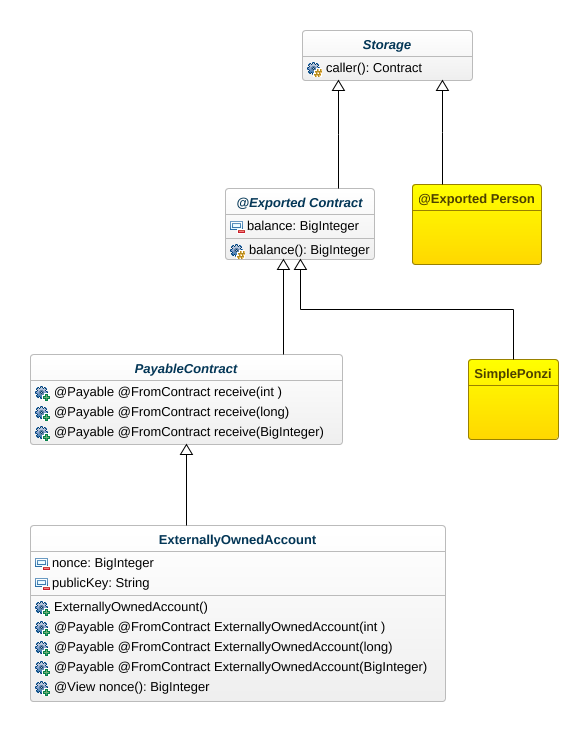
\includegraphics[width=1.05\textwidth,height=\textheight]{pics/contracts.png}
\caption{Figure 7. The hierarchy of contract classes.}
\end{figure}

The abstract subclass \texttt{PayableContract} is meant for contracts
that can receive coins from other contracts, through their final
\texttt{receive()} methods. Its concrete subclass
\texttt{ExternallyOwnedAccount} is a payable contract that can be used
to pay for a transaction. Such \emph{accounts} are typically controlled
by humans, through a wallet, but can be subclassed and instantiated
freely in Takamaka code. Their constructors allow one to build an
externally owned account and fund it with an initial amount of coins. As
we have seen in sections \protect\hyperlink{jar-transaction}{A
Transaction that Stores a Jar in a Hotmoka Node},
\protect\hyperlink{constructor-transaction}{A Transaction that Invokes a
Constructor} and \protect\hyperlink{method-transaction}{A Transaction
that Invokes a Method}, node methods that start a transaction require to
specify a payer for that transaction. Such a payer is required to be an
instance of \texttt{ExternallyOwnedAccount}, or an exception will be
thrown. In our previous examples, the expressions
\texttt{nodeWithAccounts.account(0)} and
\texttt{nodeWithAccounts.account(1)} actually refer to
\texttt{ExternallyOwnedAccount}s created during initialization
transactions triggered inside the \texttt{InitializedNode.of()} method.
\texttt{ExternallyOwnedAccount}s have a private field \texttt{nonce}
that can be accessed through the public \texttt{@View} method
\texttt{nonce()}: it yields a \texttt{BigInteger} that specifies the
next nonce to use for the next transaction having that account as
caller. This nonce gets automatically increased after each such
transaction.

Instances of \texttt{ExternallyOwnedAccount}s hold their public key in
their private \texttt{publicKey} field, that cannot be accessed
programmatically. That key is used to verify the signature of the
transactions having that account as caller. As we will se later, there
is a default signature algorithms for transactions and that is what
\texttt{ExternallyOwnedAccount}s use. However, it is possible to require
a specific signature algorithm, that overrides the default for the node.
For that, it is enough to instantiate classes
\texttt{ExternallyOwnedAccountSHA256DSA},
\texttt{ExternallyOwnedAccountED25519},
\texttt{ExternallyOwnedAccountQTESLA1} or
\texttt{ExternallyOwnedAccountQTESLA3}. The latter two use a
quantum-resistant signature algorithm (see
\protect\hyperlink{signatures-and-quantum-resistance}{Signatures and
Quantum-Resistance} for more details). This means that it is possible to
mix many signature algorithms for signing transactions inside the same
Hotmoka node, as we will show later.

\hypertarget{redgreen-contracts}{%
\section{Red/Green Contracts }\label{redgreen-contracts}}

\textbf{{[}Run \texttt{git\ checkout\ redgreen\ -\/-} inside the
\texttt{hotmoka\_tutorial} repository{]}}

Takamaka includes contract classes with double balance. They have the
normal (\emph{green}) balance and an extra, stable \emph{red} balance.
Such red/green contracts are implemented by the abstract class
\texttt{io.takamaka.code.lang.RedGreenContract}, having a subclass
\texttt{io.takamaka.code.lang.RedGreenPayableContract}, further
subclassed by
\texttt{io.takamaka.code.lang.RedGreenExternallyOwnedAccount}. That is,
such contracts have the ability to keep an extra red balance, that
should be a stable coin, if the underlying blockchain supports such
feature.

For instance, the following red/green contract allows payees to register
by calling the \texttt{addAsPayee()} method. Moreover, the contract
distributes green coins sent to the \texttt{distributeGreen()} method
and red coins sent to the \texttt{distributeRed()} method, sending the
rest to the owner of the contract (in general, there is a rest because
of arithmetic approximation). Hence, the contract holds coins only
temporarily. The \texttt{@RedPayable} annotation states that the
\texttt{distributeRed()} method transfers red coins when called. Class
\texttt{StorageLinkedList} holds a list of contracts and will be
discussed in the next chapter.

\begin{Shaded}
\begin{Highlighting}[]
\KeywordTok{package}\ImportTok{ io.takamaka.redgreen;}

\KeywordTok{import}\ImportTok{ java.math.BigInteger;}

\KeywordTok{import}\ImportTok{ io.takamaka.code.lang.FromContract;}
\KeywordTok{import}\ImportTok{ io.takamaka.code.lang.Payable;}
\KeywordTok{import}\ImportTok{ io.takamaka.code.lang.RedGreenContract;}
\KeywordTok{import}\ImportTok{ io.takamaka.code.lang.RedGreenPayableContract;}
\KeywordTok{import}\ImportTok{ io.takamaka.code.lang.RedPayable;}
\KeywordTok{import}\ImportTok{ io.takamaka.code.util.StorageLinkedList;}
\KeywordTok{import}\ImportTok{ io.takamaka.code.util.StorageList;}

\KeywordTok{public} \KeywordTok{class}\NormalTok{ Distributor }\KeywordTok{extends}\NormalTok{ RedGreenContract \{}
  \KeywordTok{private} \DataTypeTok{final}\NormalTok{ StorageList<RedGreenPayableContract> payees = }\KeywordTok{new}\NormalTok{ StorageLinkedList<>();}
  \KeywordTok{private} \DataTypeTok{final}\NormalTok{ RedGreenPayableContract owner;}

  \KeywordTok{public} \AttributeTok{@FromContract}\NormalTok{(RedGreenPayableContract.}\FunctionTok{class}\NormalTok{) }\FunctionTok{Distributor}\NormalTok{() \{}
\NormalTok{    owner = (RedGreenPayableContract) }\FunctionTok{caller}\NormalTok{();}
\NormalTok{  \}}

  \KeywordTok{public} \AttributeTok{@FromContract}\NormalTok{(RedGreenPayableContract.}\FunctionTok{class}\NormalTok{) }\DataTypeTok{void} \FunctionTok{addAsPayee}\NormalTok{() \{}
\NormalTok{    payees.}\FunctionTok{add}\NormalTok{((RedGreenPayableContract) }\FunctionTok{caller}\NormalTok{());}
\NormalTok{  \}}

  \KeywordTok{public} \AttributeTok{@Payable} \AttributeTok{@FromContract} \DataTypeTok{void} \FunctionTok{distributeGreen}\NormalTok{(}\BuiltInTok{BigInteger}\NormalTok{ amount) \{}
    \DataTypeTok{int}\NormalTok{ size = payees.}\FunctionTok{size}\NormalTok{();}
    \KeywordTok{if}\NormalTok{ (size > }\DecValTok{0}\NormalTok{) \{}
      \BuiltInTok{BigInteger}\NormalTok{ eachGets = amount.}\FunctionTok{divide}\NormalTok{(}\BuiltInTok{BigInteger}\NormalTok{.}\FunctionTok{valueOf}\NormalTok{(size));}
\NormalTok{      payees.}\FunctionTok{forEach}\NormalTok{(payee -> payee.}\FunctionTok{receive}\NormalTok{(eachGets));}
\NormalTok{      owner.}\FunctionTok{receive}\NormalTok{(}\FunctionTok{balance}\NormalTok{());}
\NormalTok{    \}}
\NormalTok{  \}}

  \KeywordTok{public} \AttributeTok{@RedPayable} \AttributeTok{@FromContract} \DataTypeTok{void} \FunctionTok{distributeRed}\NormalTok{(}\BuiltInTok{BigInteger}\NormalTok{ amount) \{}
    \DataTypeTok{int}\NormalTok{ size = payees.}\FunctionTok{size}\NormalTok{();}
    \KeywordTok{if}\NormalTok{ (size > }\DecValTok{0}\NormalTok{) \{}
      \BuiltInTok{BigInteger}\NormalTok{ eachGets = amount.}\FunctionTok{divide}\NormalTok{(}\BuiltInTok{BigInteger}\NormalTok{.}\FunctionTok{valueOf}\NormalTok{(size));}
\NormalTok{      payees.}\FunctionTok{forEach}\NormalTok{(payee -> payee.}\FunctionTok{receiveRed}\NormalTok{(eachGets));}
\NormalTok{      owner.}\FunctionTok{receiveRed}\NormalTok{(}\FunctionTok{balanceRed}\NormalTok{());}
\NormalTok{    \}}
\NormalTok{  \}}
\NormalTok{\}}
\end{Highlighting}
\end{Shaded}

\hypertarget{the-support-library}{%
\chapter{The Support Library }\label{the-support-library}}

This chapter presents the support library of the Takamaka language, that
contains classes for simplifying the definition of smart contracts.

In \protect\hyperlink{storage-types}{Storage Types and Constraints on
Storage Classes}, we said that storage objects must obey to some
constraints. The strongest constraint is that their fields of reference
type, in turn, can only hold storage objects. In particular, arrays are
not allowed there. This can be problematic, in particular for contracts
that deal with a variable, dynamic, potentially unbound number of other
contracts.

Thus, most classes of the support library deal with such constraints, by
providing fixed or variable-sized collections that can be used in
storage objects, since they are storage objects themselves. Such utility
classes implement lists, arrays and maps and are consequently generally
described as \emph{collections}. They have the property of being storage
classes, hence their objects can be kept in the store of a Hotmoka node,
\emph{as long as only storage objects are added as elements of the
collection}. As usual with collections, these utility classes have
generic type, to implement collections of arbitrary, but fixed types.
This is not problematic, since Java (and hence Takamaka) allows generic
types.

\hypertarget{storage-lists}{%
\section{Storage Lists }\label{storage-lists}}

Lists are an ordered sequence of elements. In a list, it is typically
possible to access the first element in constant time, while accesses to
the \emph{n}th element require to scan the list from its head and
consequently have a cost proportional to \emph{n}. Because of this,
lists are \textbf{not}, in general, random-access data structures, whose
\emph{n}th element should be accessible in constant time. It is also
possible to add an element at the beginning of a list, in constant time.
The size of a list is not fixed: lists grow in size as more elements are
added.

Java has many classes for implementing lists, all subclasses of
\texttt{java.util.List\textless{}T\textgreater{}}. They can be used in
Takamaka, but not as fields of a storage class. For that, Takamaka
provides an implementation of lists with the storage class
\texttt{io.takamaka.code.util.StorageLinkedList\textless{}T\textgreater{}}.
Its instances are storage objects and can consequently be held in fields
of storage classes and can be stored in a Hotmoka node, \emph{as long as
only storage objects are added to the list}. Takamaka lists provide
constant-time access and addition to both ends of a list. We refer to
the JavaDoc of \texttt{StorageLinkedList\textless{}T\textgreater{}} for
a full description of its methods. They include methods for adding
elements to either ends of the list, for accessing and removing
elements, for iterating on a list and for building a Java array
\texttt{T{[}{]}} holding the elements of a list.

\begin{figure}
\centering
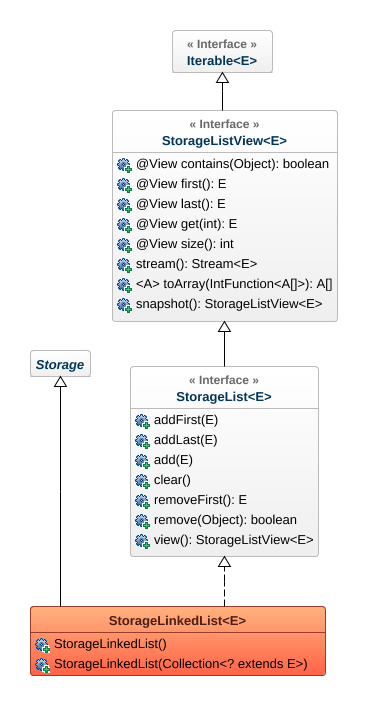
\includegraphics[width=0.5\textwidth,height=\textheight]{pics/lists.png}
\caption{Figure 8. The hierarchy of storage lists.}
\end{figure}

Figure 8 shows the hierarchy of the
\texttt{StorageLinkedList\textless{}T\textgreater{}} class. It
implements the interface \texttt{StorageList\textless{}E\textgreater{}},
that defines the methods that modify a list. That interface extends the
interface \texttt{StorageListView\textless{}E\textgreater{}} that,
instead, defines the methods that read data from a list, but do not
modify it. This distinction between the \emph{read-only} interface and
the \emph{modification} interface is typical of all collection classes
in the Takamaka library, as we will see. For the moment, note that this
distinction is useful for defining methods \texttt{snapshot()} and
\texttt{view()}. Both return a
\texttt{StorageListView\textless{}E\textgreater{}} but there is an
important difference between them. Namely, \texttt{snapshot()} yields a
\emph{frozen} view of the list, that cannot and will never be modified,
also if the original list gets updated. Instead, \texttt{view()} yields
a \emph{view} of a list, that is, a read-only list that changes whenever
the original list changes and exactly in the same way: if an element is
added to the original list, the same automatically occurs to the view.
In this sense, a view is just a read-only alias of the original list.
Both methods can be useful to export data, safely, from a node to the
outside world, since both methods return an \texttt{@Exported} object
without modification methods. Method \texttt{snapshot()} runs in linear
time (in the length of the list) while method \texttt{view()} runs in
constant time.

\begin{quote}
It might seem that \texttt{view()} is just an upwards cast to the
interface \texttt{StorageListView\textless{}E\textgreater{}}. This is
wrong, since that method does much more. Namely, it applies the façade
design pattern to provide a \emph{distinct} list that lacks any
modification method and implements a façade of the original list. To
appreciate the difference to a cast, assume to have a
\texttt{StorageList\textless{}E\textgreater{}\ list} and to write
\texttt{StorageListView\textless{}E\textgreater{}\ view\ =\ (StorageListView\textless{}E\textgreater{})\ list}.
This upwards cast will always succeed. Variable \texttt{view} does not
allow to call any modification method, since they are not in its type
\texttt{StorageListView\textless{}E\textgreater{}}. But a downwards cast
back to \texttt{StorageList\textless{}E\textgreater{}} is enough to
circumvent that constraint:
\texttt{StorageList\textless{}E\textgreater{}\ list2\ =\ (StorageList\textless{}E\textgreater{})\ view}.
This way, the original \texttt{list} can be modified by modifying
\texttt{list2} and it would not be safe to export \texttt{view}, since
it is a Trojan horse for the modification of \texttt{list}. With method
\texttt{view()}, the problem does not arise, since the cast
\texttt{StorageList\textless{}E\textgreater{}\ list2\ =\ (StorageList\textless{}E\textgreater{})\ list.view()}
fails: method \texttt{view()} actually returns another list object
without modification methods. The same is true for method
\texttt{snapshot()} that, moreover, yields a frozen view of the original
list. These same considerations hold for the other Takamaka collections
that we will see in this chapter.
\end{quote}

Next section shows an example of use for \texttt{StorageLinkedList}.

\hypertarget{a-gradual-ponzi-contract}{%
\subsection{A Gradual Ponzi Contract }\label{a-gradual-ponzi-contract}}

\textbf{{[}Run \texttt{git\ checkout\ ponzi\_gradual\ -\/-} inside the
\texttt{hotmoka\_tutorial} repository{]}}

Consider our previous Ponzi contract again. It is somehow irrealistic,
since an investor gets its investment back in full. In a more realistic
scenario, the investor will receive the investment back gradually, as
soon as new investors arrive. This is more complex to program, since the
Ponzi contract must take note of all investors that invested up to now,
not just of the current one as in \texttt{SimplePonzi.java}. This
requires a list of investors, of unbounded size. An implementation of
this gradual Ponzi contract is reported below and has been inspired by a
similar Ethereum contract from Iyer and Dannen, shown at page 150 of
\protect\hyperlink{IyerD08}{{[}IyerD08{]}}. Write its code inside
package \texttt{it.takamaka.ponzi} of the \texttt{ponzi} project, as a
new class \texttt{GradualPonzi.java}:

\begin{Shaded}
\begin{Highlighting}[]
\KeywordTok{package}\ImportTok{ io.takamaka.ponzi;}

\KeywordTok{import static}\ImportTok{ io.takamaka.code.lang.Takamaka.require;}

\KeywordTok{import}\ImportTok{ java.math.BigInteger;}

\KeywordTok{import}\ImportTok{ io.takamaka.code.lang.Contract;}
\KeywordTok{import}\ImportTok{ io.takamaka.code.lang.FromContract;}
\KeywordTok{import}\ImportTok{ io.takamaka.code.lang.Payable;}
\KeywordTok{import}\ImportTok{ io.takamaka.code.lang.PayableContract;}
\KeywordTok{import}\ImportTok{ io.takamaka.code.util.StorageLinkedList;}
\KeywordTok{import}\ImportTok{ io.takamaka.code.util.StorageList;}

\KeywordTok{public} \KeywordTok{class}\NormalTok{ GradualPonzi }\KeywordTok{extends}\NormalTok{ Contract \{}
  \KeywordTok{public} \DataTypeTok{final} \BuiltInTok{BigInteger}\NormalTok{ MINIMUM_INVESTMENT = }\BuiltInTok{BigInteger}\NormalTok{.}\FunctionTok{valueOf}\NormalTok{(}\DecValTok{1_000L}\NormalTok{);}

  \CommentTok{/**}
   \CommentTok{*}\NormalTok{ All investors up to now}\CommentTok{. }\NormalTok{This list might contain the same investor many times}\CommentTok{,}
   \CommentTok{*}\NormalTok{ which is important to pay him back more than investors who only invested once}\CommentTok{.}
   \CommentTok{*/}
  \KeywordTok{private} \DataTypeTok{final}\NormalTok{ StorageList<PayableContract> investors = }\KeywordTok{new}\NormalTok{ StorageLinkedList<>();}

  \KeywordTok{public} \AttributeTok{@FromContract}\NormalTok{(PayableContract.}\FunctionTok{class}\NormalTok{) }\FunctionTok{GradualPonzi}\NormalTok{() \{}
\NormalTok{    investors.}\FunctionTok{add}\NormalTok{((PayableContract) }\FunctionTok{caller}\NormalTok{());}
\NormalTok{  \}}

  \KeywordTok{public} \AttributeTok{@Payable} \AttributeTok{@FromContract}\NormalTok{(PayableContract.}\FunctionTok{class}\NormalTok{) }\DataTypeTok{void} \FunctionTok{invest}\NormalTok{(}\BuiltInTok{BigInteger}\NormalTok{ amount) \{}
    \FunctionTok{require}\NormalTok{(amount.}\FunctionTok{compareTo}\NormalTok{(MINIMUM_INVESTMENT) >= }\DecValTok{0}\NormalTok{,}
\NormalTok{      () -> }\StringTok{"you must invest at least "}\NormalTok{ + MINIMUM_INVESTMENT);}
    \BuiltInTok{BigInteger}\NormalTok{ eachInvestorGets = amount.}\FunctionTok{divide}\NormalTok{(}\BuiltInTok{BigInteger}\NormalTok{.}\FunctionTok{valueOf}\NormalTok{(investors.}\FunctionTok{size}\NormalTok{()));}
\NormalTok{    investors.}\FunctionTok{stream}\NormalTok{().}\FunctionTok{forEachOrdered}\NormalTok{(investor -> investor.}\FunctionTok{receive}\NormalTok{(eachInvestorGets));}
\NormalTok{    investors.}\FunctionTok{add}\NormalTok{((PayableContract) }\FunctionTok{caller}\NormalTok{());}
\NormalTok{  \}}
\NormalTok{\}}
\end{Highlighting}
\end{Shaded}

The constructor of \texttt{GradualPonzi} is annotated as
\texttt{@FromContract}, hence it can only be called by a contract, that
gets added, as first investor, in the
\texttt{io.takamaka.code.util.StorageLinkedList} held in field
\texttt{investors}. This list, that implements an unbounded list of
objects, is a storage object, as long as only storage objects are added
inside it. \texttt{PayableContract}s are storage objects, hence its use
is correct here. Subsequently, other contracts can invest by calling
method \texttt{invest()}. A minimum investment is required, but this
remains constant over time. The \texttt{amount} invested gets split by
the number of the previous investors and sent back to each of them. Note
that Takamaka allows programmers to use Java 8 lambdas and streams. Old
fashioned Java programmers, who don't feel at home with such treats, can
exploit the fact that storage lists are iterable and replace the
single-line \texttt{forEachOrdered()} call with a more traditional (but
gas-hungrier):

\begin{Shaded}
\begin{Highlighting}[]
\KeywordTok{for}\NormalTok{ (PayableContract investor: investors)}
\NormalTok{  investor.}\FunctionTok{receive}\NormalTok{(eachInvestorGets);}
\end{Highlighting}
\end{Shaded}

It is instead \textbf{highly discouraged} to iterate the list as if it
were an array. Namely, \textbf{do not write}

\begin{Shaded}
\begin{Highlighting}[]
\KeywordTok{for}\NormalTok{ (}\DataTypeTok{int}\NormalTok{ pos = }\DecValTok{0}\NormalTok{; pos < investors.}\FunctionTok{size}\NormalTok{(); pos++)}
\NormalTok{  investors.}\FunctionTok{get}\NormalTok{(i).}\FunctionTok{receive}\NormalTok{(eachInvestorGets);}
\end{Highlighting}
\end{Shaded}

since linked lists are not random-access data structures and the
complexity of the last loop is quadratic in the size of the list. This
is not a novelty: the same occurs with many traditional Java lists, that
do not implement \texttt{java.util.RandomAccess} (a notable example is
\texttt{java.util.LinkedList}). In Takamaka, code execution costs gas
and computational complexity does matter, more than in other programming
contexts.

\hypertarget{a-note-on-re-entrancy}{%
\subsection{A Note on Re-entrancy }\label{a-note-on-re-entrancy}}

The \texttt{GradualPonzi.java} class pays back previous investors
immediately: as soon as a new investor invests something, his investment
gets split and forwarded to all previous investors. This should make
Solidity programmers uncomfortable, since the same approach, in
Solidity, might lead to the infamous re-entrancy attack, when the
contract that receives his investment back has a fallback function
redefined in such a way to re-enter the paying contract and re-execute
the distribution of the investment. As it is well known, such an attack
has made some people rich and other desperate. You can find more detail
at page 173 of
\protect\hyperlink{AntonopoulosW19}{{[}AntonopoulosW19{]}}. Even if such
a frightening scenario does not occur, paying back previous investors
immediately is discouraged in Solidity also for other reasons. Namely,
the contract that receives his investment back might have a redefined
fallback function that consumes too much gas or does not terminate. This
would hang the loop that pays back previous investors, actually locking
the money inside the \texttt{GradualPonzi} contract. Moreover, paying
back a contract is a relatively expensive operation in Solidity, even if
the fallback function is not redefined, and this cost is paid by the new
investor that called \texttt{invest()}, in terms of gas. The cost is
linear in the number of investors that must be paid back.

As a solution to these problems, Solidity programmers do not pay
previous investors back immediately, but let the \texttt{GradualPonzi}
contract take note of the balance of each investor, through a map. This
map is updated as soon as a new investor arrives, by increasing the
balance of every previous investor. The cost of updating the balances is
still linear in the number of previous investors, but it is cheaper (in
Solidity) than sending money back to each of them, which requires costy
inter-contract calls that trigger new subtransactions. With this
technique, previous investors are now required to withdraw their balance
explicitly and voluntarily, through a call to some function, typically
called \texttt{widthdraw()}. This leads to the \emph{withdrawal
pattern}, widely used for writing Solidity contracts.

We have not used the withdrawal pattern in \texttt{GradualPonzi.java}.
In general, there is no need for such pattern in Takamaka, at least not
for simple contracts like \texttt{GradualPonzi.java}. The reason is that
the \texttt{receive()} methods of a payable contract (corresponding to
the fallback function of Solidity) are \texttt{final} in Takamaka and
very cheap in terms of gas. In particular, inter-contract calls are not
especially expensive in Takamaka, since they are just a method
invocation in Java bytecode (one bytecode instruction). They are
\emph{not} new transactions. They are actually cheaper than updating a
map of balances. Moreover, avoiding the \texttt{widthdraw()}
transactions means reducing the overall number of transactions; without
using the map supporting the withdrawal pattern, Takamaka contracts
consume less gas and less storage. Hence, the withdrawal pattern is both
useless in Takamaka and more expensive than paying back previous
contracts immediately.

\hypertarget{running-the-gradual-ponzi-contract}{%
\subsection{Running the Gradual Ponzi Contract
}\label{running-the-gradual-ponzi-contract}}

\textbf{{[}Run \texttt{git\ checkout\ ponzi\_gradual\_run\ -\/-} inside
the \texttt{hotmoka\_tutorial} repository{]}}

Let us play with the \texttt{GradualPonzi} contract now. Run, inside
that \texttt{ponzi} project, the command \texttt{mvn\ package}. A file
\texttt{ponzi-0.0.1-SNAPSHOT.jar} should appear inside \texttt{target}.

Go now to the \texttt{blockchain} project and create a package
\texttt{io.takamaka.ponzi} inside it. Copy the following code as
\texttt{Main.java} inside that package. Its goal is to

\begin{enumerate}
\def\labelenumi{\arabic{enumi}.}
\tightlist
\item
  install \texttt{ponzi-0.0.1-SNAPSHOT.jar} in the store of the node
\item
  create three players (that is, accounts)
\item
  let the first player create an instance of \texttt{GradualPonzi} in
  the node and become the first investor of the contract
\item
  let the other two players invest, in sequence, in the
  \texttt{GradualPonzi} contract
\item
  let the first player try to invest again in the contract, this time
  with a too small investment, which leads to an exception, since the
  code of the contract requires a minimum investment.
\end{enumerate}

\begin{Shaded}
\begin{Highlighting}[]
\KeywordTok{package}\ImportTok{ io.takamaka.ponzi;}

\KeywordTok{import static}\ImportTok{ java.math.BigInteger.ONE;}
\KeywordTok{import static}\ImportTok{ java.math.BigInteger.ZERO;}

\KeywordTok{import}\ImportTok{ java.math.BigInteger;}
\KeywordTok{import}\ImportTok{ java.nio.file.Path;}
\KeywordTok{import}\ImportTok{ java.nio.file.Paths;}

\KeywordTok{import}\ImportTok{ io.hotmoka.beans.references.TransactionReference;}
\KeywordTok{import}\ImportTok{ io.hotmoka.beans.requests.ConstructorCallTransactionRequest;}
\KeywordTok{import}\ImportTok{ io.hotmoka.beans.requests.InstanceMethodCallTransactionRequest;}
\KeywordTok{import}\ImportTok{ io.hotmoka.beans.requests.SignedTransactionRequest;}
\KeywordTok{import}\ImportTok{ io.hotmoka.beans.requests.SignedTransactionRequest.Signer;}
\KeywordTok{import}\ImportTok{ io.hotmoka.beans.signatures.ConstructorSignature;}
\KeywordTok{import}\ImportTok{ io.hotmoka.beans.signatures.VoidMethodSignature;}
\KeywordTok{import}\ImportTok{ io.hotmoka.beans.types.ClassType;}
\KeywordTok{import}\ImportTok{ io.hotmoka.beans.values.BigIntegerValue;}
\KeywordTok{import}\ImportTok{ io.hotmoka.beans.values.StorageReference;}
\KeywordTok{import}\ImportTok{ io.hotmoka.crypto.SignatureAlgorithm;}
\KeywordTok{import}\ImportTok{ io.hotmoka.memory.MemoryBlockchain;}
\KeywordTok{import}\ImportTok{ io.hotmoka.memory.MemoryBlockchainConfig;}
\KeywordTok{import}\ImportTok{ io.hotmoka.nodes.Node;}
\KeywordTok{import}\ImportTok{ io.hotmoka.nodes.views.InitializedNode;}
\KeywordTok{import}\ImportTok{ io.hotmoka.nodes.views.NodeWithAccounts;}
\KeywordTok{import}\ImportTok{ io.hotmoka.nodes.views.NodeWithJars;}

\KeywordTok{public} \KeywordTok{class}\NormalTok{ Main \{}
  \KeywordTok{public} \DataTypeTok{final} \DataTypeTok{static} \BuiltInTok{BigInteger}\NormalTok{ GREEN_AMOUNT = }\BuiltInTok{BigInteger}\NormalTok{.}\FunctionTok{valueOf}\NormalTok{(}\DecValTok{100_000_000}\NormalTok{);}
  \KeywordTok{public} \DataTypeTok{final} \DataTypeTok{static} \BuiltInTok{BigInteger}\NormalTok{ RED_AMOUNT = ZERO;}
  \KeywordTok{private} \DataTypeTok{final} \DataTypeTok{static} \BuiltInTok{BigInteger}\NormalTok{ _}\DecValTok{20_000}\NormalTok{ = }\BuiltInTok{BigInteger}\NormalTok{.}\FunctionTok{valueOf}\NormalTok{(}\DecValTok{20_000}\NormalTok{);}
  \KeywordTok{private} \DataTypeTok{final} \DataTypeTok{static} \BuiltInTok{BigInteger}\NormalTok{ _}\DecValTok{1_000_000}\NormalTok{ = }\BuiltInTok{BigInteger}\NormalTok{.}\FunctionTok{valueOf}\NormalTok{(}\DecValTok{1_000_000}\NormalTok{);}
  \KeywordTok{private} \DataTypeTok{final} \DataTypeTok{static}\NormalTok{ ClassType GRADUAL_PONZI}
\NormalTok{    = }\KeywordTok{new} \FunctionTok{ClassType}\NormalTok{(}\StringTok{"io.takamaka.ponzi.GradualPonzi"}\NormalTok{);}
  \KeywordTok{private} \DataTypeTok{final} \DataTypeTok{static}\NormalTok{ VoidMethodSignature gradualPonziInvest}
\NormalTok{    = }\KeywordTok{new} \FunctionTok{VoidMethodSignature}\NormalTok{(GRADUAL_PONZI, }\StringTok{"invest"}\NormalTok{, ClassType.}\FunctionTok{BIG_INTEGER}\NormalTok{);}

  \KeywordTok{public} \DataTypeTok{static} \DataTypeTok{void} \FunctionTok{main}\NormalTok{(}\BuiltInTok{String}\NormalTok{[] args) }\KeywordTok{throws} \BuiltInTok{Exception}\NormalTok{ \{}
\NormalTok{    MemoryBlockchainConfig config = }\KeywordTok{new}\NormalTok{ MemoryBlockchainConfig.}\FunctionTok{Builder}\NormalTok{().}\FunctionTok{build}\NormalTok{();}
\NormalTok{    Path takamakaCodePath = Paths.}\FunctionTok{get}\NormalTok{(}\StringTok{"../../hotmoka/modules/explicit/io-takamaka-code-1.0.0.jar"}\NormalTok{);}
\NormalTok{    Path ponziPath = Paths.}\FunctionTok{get}\NormalTok{(}\StringTok{"../ponzi/target/ponzi-0.0.1-SNAPSHOT.jar"}\NormalTok{);}

    \KeywordTok{try}\NormalTok{ (}\BuiltInTok{Node}\NormalTok{ node = MemoryBlockchain.}\FunctionTok{of}\NormalTok{(config)) \{}
\NormalTok{      InitializedNode initialized = InitializedNode.}\FunctionTok{of}
\NormalTok{        (node, takamakaCodePath, }\StringTok{"test"}\NormalTok{, GREEN_AMOUNT, RED_AMOUNT);}
      \CommentTok{// install the jar of the Ponzi contracts in the node}
\NormalTok{      NodeWithJars nodeWithJars = NodeWithJars.}\FunctionTok{of}
\NormalTok{        (node, initialized.}\FunctionTok{gamete}\NormalTok{(), initialized.}\FunctionTok{keysOfGamete}\NormalTok{().}\FunctionTok{getPrivate}\NormalTok{(),}
\NormalTok{         ponziPath);}
\NormalTok{      NodeWithAccounts nodeWithAccounts = NodeWithAccounts.}\FunctionTok{of}
\NormalTok{        (node, initialized.}\FunctionTok{gamete}\NormalTok{(), initialized.}\FunctionTok{keysOfGamete}\NormalTok{().}\FunctionTok{getPrivate}\NormalTok{(),}
\NormalTok{        _}\DecValTok{1_000_000}\NormalTok{, _}\DecValTok{1_000_000}\NormalTok{, _}\DecValTok{1_000_000}\NormalTok{);}

\NormalTok{      StorageReference player1 = nodeWithAccounts.}\FunctionTok{account}\NormalTok{(}\DecValTok{0}\NormalTok{);}
\NormalTok{      StorageReference player2 = nodeWithAccounts.}\FunctionTok{account}\NormalTok{(}\DecValTok{1}\NormalTok{);}
\NormalTok{      StorageReference player3 = nodeWithAccounts.}\FunctionTok{account}\NormalTok{(}\DecValTok{2}\NormalTok{);}
\NormalTok{      SignatureAlgorithm<SignedTransactionRequest> signature}
\NormalTok{        = node.}\FunctionTok{getSignatureAlgorithmForRequests}\NormalTok{();}
      \BuiltInTok{Signer}\NormalTok{ signerForPlayer1 = }\BuiltInTok{Signer}\NormalTok{.}\FunctionTok{with}\NormalTok{(signature, nodeWithAccounts.}\FunctionTok{privateKey}\NormalTok{(}\DecValTok{0}\NormalTok{));}
      \BuiltInTok{Signer}\NormalTok{ signarerForPlayer2 = }\BuiltInTok{Signer}\NormalTok{.}\FunctionTok{with}\NormalTok{(signature, nodeWithAccounts.}\FunctionTok{privateKey}\NormalTok{(}\DecValTok{1}\NormalTok{));}
      \BuiltInTok{Signer}\NormalTok{ signerForPlayer3 = }\BuiltInTok{Signer}\NormalTok{.}\FunctionTok{with}\NormalTok{(signature, nodeWithAccounts.}\FunctionTok{privateKey}\NormalTok{(}\DecValTok{2}\NormalTok{));}
\NormalTok{      TransactionReference classpath = nodeWithJars.}\FunctionTok{jar}\NormalTok{(}\DecValTok{0}\NormalTok{);}

      \CommentTok{// create the Ponzi contract: player1 becomes its first investor}
\NormalTok{      StorageReference gradualPonzi = node.}\FunctionTok{addConstructorCallTransaction}
\NormalTok{        (}\KeywordTok{new} \FunctionTok{ConstructorCallTransactionRequest}\NormalTok{(}
\NormalTok{          signerForPlayer1,}
\NormalTok{          player1, }\CommentTok{// player1 pays for the transaction}
\NormalTok{          ZERO, }\CommentTok{// nonce for player1}
          \StringTok{"test"}\NormalTok{, }\CommentTok{// chain identifier}
\NormalTok{          _}\DecValTok{20_000}\NormalTok{, }\CommentTok{// gas provided to the transaction}
\NormalTok{          ONE, }\CommentTok{// gas price}
\NormalTok{          classpath,}
          \KeywordTok{new} \FunctionTok{ConstructorSignature}\NormalTok{(GRADUAL_PONZI))); }\CommentTok{/// GradualPonzi()}

      \CommentTok{// let player2 invest 1200}
\NormalTok{      node.}\FunctionTok{addInstanceMethodCallTransaction}\NormalTok{(}\KeywordTok{new} \FunctionTok{InstanceMethodCallTransactionRequest}\NormalTok{(}
\NormalTok{        signarerForPlayer2,}
\NormalTok{        player2, }\CommentTok{// player2 pays for the transaction}
\NormalTok{        ZERO, }\CommentTok{// nonce for player2}
        \StringTok{"test"}\NormalTok{, }\CommentTok{// chain identifier}
\NormalTok{        _}\DecValTok{20_000}\NormalTok{, }\CommentTok{// gas provided to the transaction}
\NormalTok{        ONE, }\CommentTok{// gas price}
\NormalTok{        classpath,}
\NormalTok{        gradualPonziInvest, }\CommentTok{// method void GradualPonzi.invest(BigInteger)}
\NormalTok{        gradualPonzi, }\CommentTok{// receiver of invest()}
        \KeywordTok{new} \FunctionTok{BigIntegerValue}\NormalTok{(}\BuiltInTok{BigInteger}\NormalTok{.}\FunctionTok{valueOf}\NormalTok{(}\DecValTok{1_200}\NormalTok{)))); }\CommentTok{// the investment}

      \CommentTok{// let player3 invest 1500}
\NormalTok{      node.}\FunctionTok{addInstanceMethodCallTransaction}\NormalTok{(}\KeywordTok{new} \FunctionTok{InstanceMethodCallTransactionRequest}\NormalTok{(}
\NormalTok{        signerForPlayer3,}
\NormalTok{        player3, }\CommentTok{// player3 pays for the transaction}
\NormalTok{        ZERO, }\CommentTok{// nonce of player3}
        \StringTok{"test"}\NormalTok{, }\CommentTok{// chain identifier}
\NormalTok{        _}\DecValTok{20_000}\NormalTok{, }\CommentTok{// gas provided to the transaction}
\NormalTok{        ONE, }\CommentTok{// gas price}
\NormalTok{        classpath,}
\NormalTok{        gradualPonziInvest, }\CommentTok{// method void GradualPonzi.invest(BigInteger)}
\NormalTok{        gradualPonzi, }\CommentTok{// receiver of invest()}
        \KeywordTok{new} \FunctionTok{BigIntegerValue}\NormalTok{(}\BuiltInTok{BigInteger}\NormalTok{.}\FunctionTok{valueOf}\NormalTok{(}\DecValTok{1_500}\NormalTok{)))); }\CommentTok{// the investment}

      \CommentTok{// let player1 invest 900, but it is too little and it runs into an exception}
\NormalTok{      node.}\FunctionTok{addInstanceMethodCallTransaction}\NormalTok{(}\KeywordTok{new} \FunctionTok{InstanceMethodCallTransactionRequest}\NormalTok{(}
\NormalTok{        signerForPlayer1,}
\NormalTok{        player1, }\CommentTok{// player1 pays for the transaction}
\NormalTok{        ONE, }\CommentTok{// nonce of player1}
        \StringTok{"test"}\NormalTok{, }\CommentTok{// chain identifier}
\NormalTok{        _}\DecValTok{20_000}\NormalTok{, }\CommentTok{// gas provided to the transaction}
\NormalTok{        ONE, }\CommentTok{// gas price}
\NormalTok{        classpath,}
\NormalTok{        gradualPonziInvest, }\CommentTok{// method void GradualPonzi.invest(BigInteger)}
\NormalTok{        gradualPonzi, }\CommentTok{// receiver of invest()}
        \KeywordTok{new} \FunctionTok{BigIntegerValue}\NormalTok{(}\BuiltInTok{BigInteger}\NormalTok{.}\FunctionTok{valueOf}\NormalTok{(}\DecValTok{900}\NormalTok{)))); }\CommentTok{// the investment}
\NormalTok{    \}}
\NormalTok{  \}}
\NormalTok{\}}
\end{Highlighting}
\end{Shaded}

Package the \texttt{blockchain} project and run the above
\texttt{Main.java} (the \texttt{java} invocation command is on a single
line):

\begin{myverbatim}
\begin{verbatim}
$ cd blockchain
$ mvn package
$ java --module-path $explicit:$automatic:target/blockchain-0.0.1-SNAPSHOT.jar
       -classpath $unnamed"/*"
       --module blockchain/io.takamaka.ponzi.Main
\end{verbatim}
\end{myverbatim}

The result will be to execute a sequence of transactions that create and
invest in the contract, until the last transaction, that ends up in an
exception:

\begin{myverbatim}
\begin{verbatim}
Exception in thread "main"
  io.hotmoka.beans.TransactionException:
  io.takamaka.code.lang.RequirementViolationException:
  you must invest at least 1000@GradualPonzi.java:28
    at...
\end{verbatim}
\end{myverbatim}

This exception states that a transaction failed because some investor
invested less than 1,000 units of coin. Note that the exception message
reports the cause (a \texttt{require} failed) and includes the source
program line of the contract where the exception occurred: line 28 of
\texttt{GradualPonzi.java}, that is

\begin{Shaded}
\begin{Highlighting}[]
\FunctionTok{require}\NormalTok{(amount.}\FunctionTok{compareTo}\NormalTok{(MINIMUM_INVESTMENT) >= }\DecValTok{0}\NormalTok{,}
\NormalTok{  () -> }\StringTok{"you must invest at least "}\NormalTok{ + MINIMUM_INVESTMENT);}
\end{Highlighting}
\end{Shaded}

It is interesting to look at the response of the transaction where the
third player invested 1500 coins: \texttt{b2/1-.../response.txt}:

\begin{myverbatim}
\begin{verbatim}
VoidMethodCallTransactionSuccessfulResponse:
  gas consumed for CPU execution: 1014
  gas consumed for RAM allocation: 1426
  gas consumed for storage consumption: 340
  updates:
    <12314ee004bf182f0be54bf53c7e82e48bbebdd37dccdcf4b24187b675ad7064#0.class
      |io.takamaka.code.util.StorageLinkedList$Node
      |@a18c0aebf58cdc6b1c9de40baea748f9507638744ee21226ede2be1e94f2be72>
    <81664cc5a41d1af8873a019c751a5f83638657172482043fcc4a115bb7b91499#0
      |io.takamaka.code.lang.Contract.balance:java.math.BigInteger|997116>
    <e255b986b7a4e20b11d0282c031802f023f9e425dfca2625714e87c97615847a#0
      |io.takamaka.code.lang.Contract.balance:java.math.BigInteger|995720>
    <f0b4ad199d74aed8e4d548bb8e243c7d2f2fa9d2144e331dad27a97696c79cdd#0
      |io.takamaka.code.lang.Contract.balance:java.math.BigInteger|998464>
    <7a5b7e22ed3b8a4aa2fe9b443e0ef73d87eedcf562361712e10cc7ca3cfbbb1b#1
      |io.takamaka.code.util.StorageLinkedList.size:int|3>
    <e255b986b7a4e20b11d0282c031802f023f9e425dfca2625714e87c97615847a#0
      |io.takamaka.code.lang.ExternallyOwnedAccount.nonce:java.math.BigInteger|1>
    <12314ee004bf182f0be54bf53c7e82e48bbebdd37dccdcf4b24187b675ad7064#0
      |io.takamaka.code.util.StorageLinkedList$Node.element:java.lang.Object
      |e255b986b7a4e20b11d0282c031802f023f9e425dfca2625714e87c97615847a#0>
    <7a5b7e22ed3b8a4aa2fe9b443e0ef73d87eedcf562361712e10cc7ca3cfbbb1b#1
      |io.takamaka.code.util.StorageLinkedList.last
        :io.takamaka.code.util.StorageList$Node
      |12314ee004bf182f0be54bf53c7e82e48bbebdd37dccdcf4b24187b675ad7064#0>
    <d8da00750d67aa7c807b98e86d9629ec43e6427c094efdc7e970315683123cf6#0
      |io.takamaka.code.util.StorageLinkedList$Node.next
        :io.takamaka.code.util.StorageLinkedList$Node
      |12314ee004bf182f0be54bf53c7e82e48bbebdd37dccdcf4b24187b675ad7064#0>
    <12314ee004bf182f0be54bf53c7e82e48bbebdd37dccdcf4b24187b675ad7064#0
      |io.takamaka.code.util.StorageLinkedList$Node.next
        :io.takamaka.code.util.StorageLinkedList$Node
      |null>
  events:
\end{verbatim}
\end{myverbatim}

The third player
\texttt{e255b986b7a4e20b11d0282c031802f023f9e425dfca2625714e87c97615847a\#0}
sees its balance updated since it paid for the transaction and invested
money, that got distributed to
\texttt{81664cc5a41d1af8873a019c751a5f83638657172482043fcc4a115bb7b91499\#0}
and
\texttt{f0b4ad199d74aed8e4d548bb8e243c7d2f2fa9d2144e331dad27a97696c79cdd\#0},
that are the other two players. The storage list containing the
investors, that is the storage object
\texttt{7a5b7e22ed3b8a4aa2fe9b443e0ef73d87eedcf562361712e10cc7ca3cfbbb1b\#1},
sees its size become 3 with this transaction. You can see that the
transaction creates and updates many objects, that are used internally
to represent the nodes of the list.

\hypertarget{storage-arrays}{%
\section{Storage Arrays }\label{storage-arrays}}

Arrays are an ordered sequence of elements, with constant-time access to
such elements, both for reading and for writing. The size of the arrays
is typically fixed, although there are programming languages with
limited forms of dynamic arrays.

Java has native arrays, of type \texttt{E{[}{]}}, where \texttt{E} is
the type of the elements of the array. They can be used in Takamaka, but
not as fields of storage classes. For that, Takamaka provides class
\texttt{io.takamaka.code.util.StorageTreeArray\textless{}E\textgreater{}}.
Its instances are storage objects and can consequently be held in fields
of storage classes and can be stored in the store of a Hotmoka node,
\emph{as long as only storage objects are added to the array}. Their
size is fixed and decided at time of construction. Although we consider
\texttt{StorageTreeArray\textless{}E\textgreater{}} as the storage
replacement for Java arrays, it must be stated that the complexity of
accessing their elements is logarithmic in the size of the array, which
is a significant deviation from the standard definition of arrays.
Nevertheless, logarithmic complexity is much better than the linear
complexity for accessing elements of a
\texttt{StorageLinkedList\textless{}E\textgreater{}} that, instead, has
the advantage of being dynamic in size.

\begin{figure}
\centering
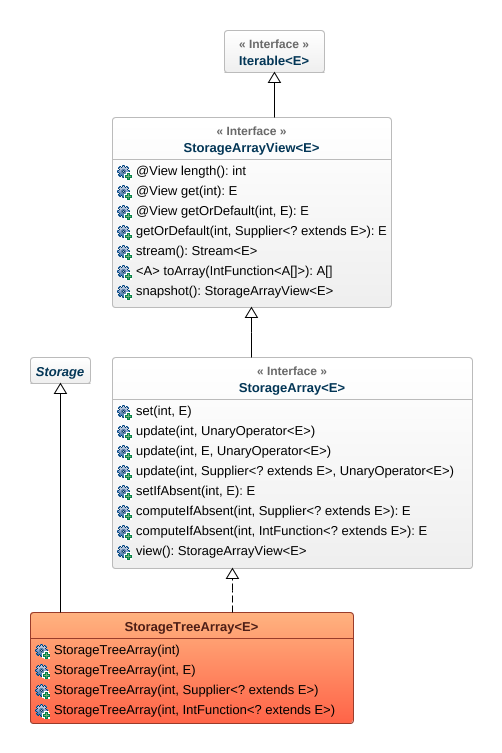
\includegraphics[width=0.65\textwidth,height=\textheight]{pics/arrays.png}
\caption{Figure 9. The hierarchy of storage arrays.}
\end{figure}

We refer to the JavaDoc of
\texttt{StorageTreeArray\textless{}E\textgreater{}} for a full list of
its methods. They include methods for adding elements, for accessing and
removing elements, for iterating on an array and for building a Java
array \texttt{E{[}{]}} with the elements of a
\texttt{StorageTreeArray\textless{}E\textgreater{}}. Figure 9 shows the
hierarchy of the \texttt{StorageTreeArray\textless{}E\textgreater{}}
class. It implements the interface
\texttt{StorageArray\textless{}E\textgreater{}}, that defines the
methods that modify an array. That interface extends the interface
\texttt{StorageArrayView\textless{}E\textgreater{}} that, instead,
defines the methods that read data from an array, but do not modify it.
This distinction between the \emph{read-only} interface and the
\emph{modification} interface is identical to what we have seen for
lists in the previous sections. Arrays have methods \texttt{snapshot()}
and \texttt{view()} as weel, like lists. They yield \texttt{@Exported}
objects. All constructors of the
\texttt{StorageTreeArray\textless{}E\textgreater{}} class require to
specify the immutable size of the array. Moreover, it is possible to
specify a default value for the elements of the array, that can be
explicit or given as a supplier, possibly indexed. Methods
\texttt{snapshot()} and \texttt{view()} return an \texttt{@Exported}
storage array, in constant time.

Next section shows an example of use for
\texttt{StorageTreeArray\textless{}T\textgreater{}}.

\hypertarget{a-tic-tac-toe-contract}{%
\subsection{A Tic-Tac-Toe Contract }\label{a-tic-tac-toe-contract}}

\textbf{{[}Run \texttt{git\ checkout\ tictactoe\ -\/-} inside the
\texttt{hotmoka\_tutorial} repository{]}}

Tic-tac-toe is a two-players game where players place, alternately, a
cross and a circle on a 3x3 board, initially empty. The winner is the
player who places three crosses or three circles on the same row, column
or diagonal. For instance, in Figure 10 the player of the cross wins.

\begin{figure}
\centering

\includegraphics[width=0.3\textwidth,height=\textheight]{pics/tictactoe_wins.png}
\caption{Figure 10. Cross wins.}
\end{figure}

There are games that end up in a draw, when the board is full but nobody
wins, as in Figure 11.

\begin{figure}
\centering
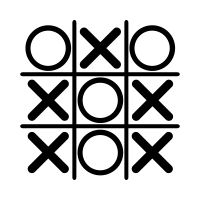
\includegraphics[width=0.39\textwidth,height=\textheight]{pics/tictactoe_draw.png}
\caption{Figure 11. A draw.}
\end{figure}

A natural representation of the tic-tac-toe board is a bidimensional
array where indexes are distributed as shown in Figure 12.

\begin{figure}
\centering
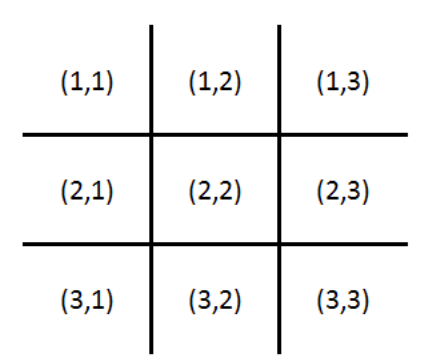
\includegraphics[width=0.35\textwidth,height=\textheight]{pics/tictactoe_grid.png}
\caption{Figure 12. A bidimensional representation of the game.}
\end{figure}

This can be implemented as a
\texttt{StorageTreeArray\textless{}StorageTreeArray\textless{}Tile\textgreater{}\textgreater{}},
where \texttt{Tile} is an enumeration of the three possible tiles
(empty, cross, circle). This is possible but overkill. It is simpler and
cheaper (also in terms of gas) to use the previous diagram as a
conceptual representation of the board shown to the users, but use,
internally, a monodimensional array of nine tiles, distributed as
follows:

\begin{figure}
\centering
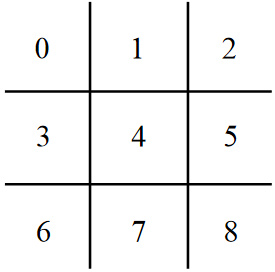
\includegraphics[width=0.3\textwidth,height=\textheight]{pics/tictactoe_grid_linear.png}
\caption{Figure 13. A linear representation of the game.}
\end{figure}

that can be implemented as a
\texttt{StorageTreeArray\textless{}Tile\textgreater{}}. There will be
functions for translating the conceptual representation into the
internal one.

Create hence in Eclipse a new Maven Java 11 (or later) project named
\texttt{tictactoe}. You can do this by duplicating the project
\texttt{family} (make sure to store the project inside the
\texttt{hotmoka} directory, as a sibling of \texttt{family},
\texttt{ponzi} and \texttt{blockchain}). Use the following
\texttt{pom.xml}:

\begin{Shaded}
\begin{Highlighting}[]
\KeywordTok{<project}\OtherTok{ xmlns=}\StringTok{"http://maven.apache.org/POM/4.0.0"}
\OtherTok{    xmlns:xsi=}\StringTok{"http://www.w3.org/2001/XMLSchema-instance"}
\OtherTok{    xsi:schemaLocation=}\StringTok{"http://maven.apache.org/POM/4.0.0}
\StringTok{    http://maven.apache.org/xsd/maven-4.0.0.xsd"}\KeywordTok{>}

  \KeywordTok{<modelVersion>}\NormalTok{4.0.0}\KeywordTok{</modelVersion>}
  \KeywordTok{<groupId>}\NormalTok{io.hotmoka}\KeywordTok{</groupId>}
  \KeywordTok{<artifactId>}\NormalTok{tictactoe}\KeywordTok{</artifactId>}
  \KeywordTok{<version>}\NormalTok{0.0.1-SNAPSHOT}\KeywordTok{</version>}

  \KeywordTok{<properties>}
    \KeywordTok{<project.build.sourceEncoding>}\NormalTok{UTF-8}\KeywordTok{</project.build.sourceEncoding>}
    \KeywordTok{<maven.compiler.source>}\NormalTok{11}\KeywordTok{</maven.compiler.source>}
    \KeywordTok{<maven.compiler.target>}\NormalTok{11}\KeywordTok{</maven.compiler.target>}
    \KeywordTok{<failOnMissingWebXml>}\NormalTok{false}\KeywordTok{</failOnMissingWebXml>}
  \KeywordTok{</properties>}

  \KeywordTok{<dependencies>}
    \KeywordTok{<dependency>}
      \KeywordTok{<groupId>}\NormalTok{io.hotmoka}\KeywordTok{</groupId>}
      \KeywordTok{<artifactId>}\NormalTok{io-takamaka-code}\KeywordTok{</artifactId>}
      \KeywordTok{<version>}\NormalTok{1.0.0}\KeywordTok{</version>}
    \KeywordTok{</dependency>}
  \KeywordTok{</dependencies>}

  \KeywordTok{<build>}
    \KeywordTok{<plugins>}
      \KeywordTok{<plugin>}
        \KeywordTok{<groupId>}\NormalTok{org.apache.maven.plugins}\KeywordTok{</groupId>}
        \KeywordTok{<artifactId>}\NormalTok{maven-compiler-plugin}\KeywordTok{</artifactId>}
        \KeywordTok{<version>}\NormalTok{3.8.1}\KeywordTok{</version>}
        \KeywordTok{<configuration>}
          \KeywordTok{<release>}\NormalTok{11}\KeywordTok{</release>}
        \KeywordTok{</configuration>}
      \KeywordTok{</plugin>}
    \KeywordTok{</plugins>}
  \KeywordTok{</build>}

\KeywordTok{</project>}
\end{Highlighting}
\end{Shaded}

and the following \texttt{module-info.java}:

\begin{Shaded}
\begin{Highlighting}[]
\NormalTok{module tictactoe \{}
\NormalTok{  requires io.}\FunctionTok{takamaka}\NormalTok{.}\FunctionTok{code}\NormalTok{;}
\NormalTok{\}}
\end{Highlighting}
\end{Shaded}

Create package \texttt{io.takamaka.tictactoe} inside
\texttt{src/main/java} and add the following \texttt{TicTacToe.java}
source inside that package:

\begin{Shaded}
\begin{Highlighting}[]
\KeywordTok{package}\ImportTok{ io.takamaka.tictactoe;}

\KeywordTok{import static}\ImportTok{ io.takamaka.code.lang.Takamaka.require;}
\KeywordTok{import static}\ImportTok{ java.util.stream.Collectors.joining;}
\KeywordTok{import static}\ImportTok{ java.util.stream.IntStream.rangeClosed;}

\KeywordTok{import}\ImportTok{ java.math.BigInteger;}

\KeywordTok{import}\ImportTok{ io.takamaka.code.lang.Contract;}
\KeywordTok{import}\ImportTok{ io.takamaka.code.lang.FromContract;}
\KeywordTok{import}\ImportTok{ io.takamaka.code.lang.Payable;}
\KeywordTok{import}\ImportTok{ io.takamaka.code.lang.PayableContract;}
\KeywordTok{import}\ImportTok{ io.takamaka.code.lang.View;}
\KeywordTok{import}\ImportTok{ io.takamaka.code.util.StorageArray;}
\KeywordTok{import}\ImportTok{ io.takamaka.code.util.StorageTreeArray;}

\KeywordTok{public} \KeywordTok{class}\NormalTok{ TicTacToe }\KeywordTok{extends}\NormalTok{ Contract \{}

  \KeywordTok{public} \DataTypeTok{static} \KeywordTok{enum}\NormalTok{ Tile \{}
\NormalTok{    EMPTY, CROSS, CIRCLE;}

    \AttributeTok{@Override}
    \KeywordTok{public} \BuiltInTok{String} \FunctionTok{toString}\NormalTok{() \{}
      \KeywordTok{switch}\NormalTok{ (}\KeywordTok{this}\NormalTok{) \{}
      \KeywordTok{case}\NormalTok{ EMPTY: }\KeywordTok{return} \StringTok{" "}\NormalTok{;}
      \KeywordTok{case}\NormalTok{ CROSS: }\KeywordTok{return} \StringTok{"X"}\NormalTok{;}
      \KeywordTok{default}\NormalTok{: }\KeywordTok{return} \StringTok{"O"}\NormalTok{;}
\NormalTok{      \}}
\NormalTok{    \}}

    \KeywordTok{private}\NormalTok{ Tile }\FunctionTok{nextTurn}\NormalTok{() \{}
      \KeywordTok{return} \KeywordTok{this}\NormalTok{ == CROSS ? CIRCLE : CROSS;}
\NormalTok{    \}}
\NormalTok{  \}}

  \KeywordTok{private} \DataTypeTok{final}\NormalTok{ StorageArray<Tile> board = }\KeywordTok{new}\NormalTok{ StorageTreeArray<>(}\DecValTok{9}\NormalTok{, Tile.}\FunctionTok{EMPTY}\NormalTok{);}
  \KeywordTok{private}\NormalTok{ PayableContract crossPlayer, circlePlayer;}
  \KeywordTok{private}\NormalTok{ Tile turn = Tile.}\FunctionTok{CROSS}\NormalTok{; }\CommentTok{// cross plays first}
  \KeywordTok{private} \DataTypeTok{boolean}\NormalTok{ gameOver;}

  \KeywordTok{public} \AttributeTok{@View}\NormalTok{ Tile }\FunctionTok{at}\NormalTok{(}\DataTypeTok{int}\NormalTok{ x, }\DataTypeTok{int}\NormalTok{ y) \{}
    \FunctionTok{require}\NormalTok{(}\DecValTok{1}\NormalTok{ <= x && x <= }\DecValTok{3}\NormalTok{ && }\DecValTok{1}\NormalTok{ <= y && y <= }\DecValTok{3}\NormalTok{,}
      \StringTok{"coordinates must be between 1 and 3"}\NormalTok{);}
    \KeywordTok{return}\NormalTok{ board.}\FunctionTok{get}\NormalTok{((y - }\DecValTok{1}\NormalTok{) * }\DecValTok{3}\NormalTok{ + x - }\DecValTok{1}\NormalTok{);}
\NormalTok{  \}}

  \KeywordTok{private} \DataTypeTok{void} \FunctionTok{set}\NormalTok{(}\DataTypeTok{int}\NormalTok{ x, }\DataTypeTok{int}\NormalTok{ y, Tile tile) \{}
\NormalTok{    board.}\FunctionTok{set}\NormalTok{((y - }\DecValTok{1}\NormalTok{) * }\DecValTok{3}\NormalTok{ + x - }\DecValTok{1}\NormalTok{, tile);}
\NormalTok{  \}}

  \KeywordTok{public} \AttributeTok{@Payable} \AttributeTok{@FromContract}\NormalTok{(PayableContract.}\FunctionTok{class}\NormalTok{)}
      \DataTypeTok{void} \FunctionTok{play}\NormalTok{(}\DataTypeTok{long}\NormalTok{ amount, }\DataTypeTok{int}\NormalTok{ x, }\DataTypeTok{int}\NormalTok{ y) \{}

    \FunctionTok{require}\NormalTok{(!gameOver, }\StringTok{"the game is over"}\NormalTok{);}
    \FunctionTok{require}\NormalTok{(}\DecValTok{1}\NormalTok{ <= x && x <= }\DecValTok{3}\NormalTok{ && }\DecValTok{1}\NormalTok{ <= y && y <= }\DecValTok{3}\NormalTok{,}
      \StringTok{"coordinates must be between 1 and 3"}\NormalTok{);}
    \FunctionTok{require}\NormalTok{(}\FunctionTok{at}\NormalTok{(x, y) == Tile.}\FunctionTok{EMPTY}\NormalTok{, }\StringTok{"the selected tile is not empty"}\NormalTok{);}

\NormalTok{    PayableContract player = (PayableContract) }\FunctionTok{caller}\NormalTok{();}

    \KeywordTok{if}\NormalTok{ (turn == Tile.}\FunctionTok{CROSS}\NormalTok{)}
      \KeywordTok{if}\NormalTok{ (crossPlayer == }\KeywordTok{null}\NormalTok{)}
\NormalTok{        crossPlayer = player;}
      \KeywordTok{else}
        \FunctionTok{require}\NormalTok{(player == crossPlayer, }\StringTok{"it's not your turn"}\NormalTok{);}
    \KeywordTok{else}
      \KeywordTok{if}\NormalTok{ (circlePlayer == }\KeywordTok{null}\NormalTok{) \{}
        \FunctionTok{require}\NormalTok{(crossPlayer != player, }\StringTok{"you cannot play against yourself"}\NormalTok{);}
        \DataTypeTok{long}\NormalTok{ previousBet = }\FunctionTok{balance}\NormalTok{().}\FunctionTok{subtract}\NormalTok{(}\BuiltInTok{BigInteger}\NormalTok{.}\FunctionTok{valueOf}\NormalTok{(amount)).}\FunctionTok{longValue}\NormalTok{();}
        \FunctionTok{require}\NormalTok{(amount >= previousBet,}
\NormalTok{          () -> }\StringTok{"you must bet at least "}\NormalTok{ + previousBet + }\StringTok{" coins"}\NormalTok{);}
\NormalTok{        circlePlayer = player;}
\NormalTok{      \}}
      \KeywordTok{else}
        \FunctionTok{require}\NormalTok{(player == circlePlayer, }\StringTok{"it's not your turn"}\NormalTok{);}

    \FunctionTok{set}\NormalTok{(x, y, turn);}
    \KeywordTok{if}\NormalTok{ (}\FunctionTok{isGameOver}\NormalTok{(x, y))}
\NormalTok{      player.}\FunctionTok{receive}\NormalTok{(}\FunctionTok{balance}\NormalTok{());}
    \KeywordTok{else}
\NormalTok{      turn = turn.}\FunctionTok{nextTurn}\NormalTok{();}
\NormalTok{  \}}

  \KeywordTok{private} \DataTypeTok{boolean} \FunctionTok{isGameOver}\NormalTok{(}\DataTypeTok{int}\NormalTok{ x, }\DataTypeTok{int}\NormalTok{ y) \{}
    \KeywordTok{return}\NormalTok{ gameOver =}
      \FunctionTok{rangeClosed}\NormalTok{(}\DecValTok{1}\NormalTok{, }\DecValTok{3}\NormalTok{).}\FunctionTok{allMatch}\NormalTok{(_y -> }\FunctionTok{at}\NormalTok{(x, _y) == turn) || }\CommentTok{// column x}
      \FunctionTok{rangeClosed}\NormalTok{(}\DecValTok{1}\NormalTok{, }\DecValTok{3}\NormalTok{).}\FunctionTok{allMatch}\NormalTok{(_x -> }\FunctionTok{at}\NormalTok{(_x, y) == turn) || }\CommentTok{// row y}
\NormalTok{      (x == y && }\FunctionTok{rangeClosed}\NormalTok{(}\DecValTok{1}\NormalTok{, }\DecValTok{3}\NormalTok{).}\FunctionTok{allMatch}\NormalTok{(_x -> }\FunctionTok{at}\NormalTok{(_x, _x) == turn)) || }\CommentTok{// 1st diagonal}
\NormalTok{      (x + y == }\DecValTok{4}\NormalTok{ && }\FunctionTok{rangeClosed}\NormalTok{(}\DecValTok{1}\NormalTok{, }\DecValTok{3}\NormalTok{).}\FunctionTok{allMatch}\NormalTok{(_x -> }\FunctionTok{at}\NormalTok{(_x, }\DecValTok{4}\NormalTok{ - _x) == turn)); }\CommentTok{// 2nd}
\NormalTok{  \}}

  \AttributeTok{@Override}
  \KeywordTok{public} \AttributeTok{@View} \BuiltInTok{String} \FunctionTok{toString}\NormalTok{() \{}
    \KeywordTok{return} \FunctionTok{rangeClosed}\NormalTok{(}\DecValTok{1}\NormalTok{, }\DecValTok{3}\NormalTok{)}
\NormalTok{      .}\FunctionTok{mapToObj}\NormalTok{(y -> }\FunctionTok{rangeClosed}\NormalTok{(}\DecValTok{1}\NormalTok{, }\DecValTok{3}\NormalTok{)}
\NormalTok{                     .}\FunctionTok{mapToObj}\NormalTok{(x -> }\FunctionTok{at}\NormalTok{(x, y).}\FunctionTok{toString}\NormalTok{())}
\NormalTok{                     .}\FunctionTok{collect}\NormalTok{(}\FunctionTok{joining}\NormalTok{(}\StringTok{"|"}\NormalTok{)))}
\NormalTok{      .}\FunctionTok{collect}\NormalTok{(}\FunctionTok{joining}\NormalTok{(}\StringTok{"}\SpecialCharTok{\textbackslash{}n}\StringTok{-----}\SpecialCharTok{\textbackslash{}n}\StringTok{"}\NormalTok{));}
\NormalTok{  \}}
\NormalTok{\}}
\end{Highlighting}
\end{Shaded}

The internal enumeration \texttt{Tile} represents the three alternatives
that can be put in the tic-tac-toe board. It overrides the default
\texttt{toString()} implementation, to yield the usual representation
for such alternatives; its \texttt{nextTurn()} method alternates between
cross and circle.

\begin{quote}
The \texttt{Tile} enumeration has been defined as \texttt{static} since
it needn't access the external \texttt{TicTacToe} object. It is well
possible to get rid of that \texttt{static}: the contract will work
perfectly well anyway. However, adding \texttt{static} is a Java feature
that allows programmers to reduce the memory footprint of the
enumeration elements and the cost of garbage collection. In the case of
Takamaka, it also reduces the gas cost of using this enumeration, which
is probably a more convincing argument for using \texttt{static}, since
gas is money.
\end{quote}

The board of the game is represented as a
\texttt{new\ StorageTreeArray\textless{}\textgreater{}(9,\ Tile.EMPTY)},
whose elements are indexed from 0 to 8 (inclusive) and are initialized
to \texttt{Tile.EMPTY}. It is also possible to construct the array as
\texttt{new\ StorageTreeArray\textless{}Tile\textgreater{}(9)}, but then
its elements would hold the default value \texttt{null} and the array
would need to be initialized inside a constructor for
\texttt{TicTacToe}:

\begin{Shaded}
\begin{Highlighting}[]
\KeywordTok{public} \FunctionTok{TicTacToe}\NormalTok{() \{}
  \FunctionTok{rangeClosed}\NormalTok{(}\DecValTok{0}\NormalTok{, }\DecValTok{8}\NormalTok{).}\FunctionTok{forEachOrdered}\NormalTok{(index -> board.}\FunctionTok{set}\NormalTok{(index, Tile.}\FunctionTok{EMPTY}\NormalTok{));}
\NormalTok{\}}
\end{Highlighting}
\end{Shaded}

Methods \texttt{at()} and \texttt{set()} read and set the board element
at indexes (x,y), respectively. They transform the bidimensional
conceptual representation of the board into its internal monodimensional
representation. Since \texttt{at()} is \texttt{public}, we defensively
check the validity of the indexes there.

Method \texttt{play()} is the heart of the contract. It is called by the
accounts that play the game, hence is a \texttt{@FromContract}. It is
also annotated as \texttt{@Payable(PayableContract.class)} since players
must bet money for taking part in the game, at least for the first two
moves, and receive money if they win. The first contract that plays is
registered as \texttt{crossPlayer}. The second contract that plays is
registered as \texttt{circlePlayer}. Subsequent moves must come,
alternately, from \texttt{crossPlayer} and \texttt{circlePlayer}. The
contract uses a \texttt{turn} variable to keep track of the current
turn.

Note the extensive use of \texttt{require()} to check all error
situations:

\begin{enumerate}
\def\labelenumi{\arabic{enumi}.}
\tightlist
\item
  it is possible to play only if the game is not over yet;
\item
  a move must be inside the board and identify an empty tile;
\item
  players must alternate correctly;
\item
  the second player must bet at least as much as the first player;
\item
  it is not allowed to play against oneself.
\end{enumerate}

The \texttt{play()} method ends with a call to \texttt{gameOver()} that
checks if the game is over. In that case, the winner receives the full
jackpot. Note that the \texttt{gameOver()} method receives the
coordinates where the current player has moved. This allows it to
restrict the check for game over: the game is over only if the row or
column where the player moved contain the same tile; if the current
player played on a diagonal, the method checks the diagonals as well. It
is of course possible to check all rows, columns and diagonals, always,
but our solution is gas-thriftier.

The \texttt{toString()} method yields a string representation of the
current board, such as

\begin{myverbatim}
\begin{verbatim}
X|O| 
-----
 |X|O
-----
 |X| 
\end{verbatim}
\end{myverbatim}

For those who do not appreciate Java 8 streams, the same result can be
obtained with a more traditional (and gas-hungrier) code:

\begin{Shaded}
\begin{Highlighting}[]
\AttributeTok{@Override}
\KeywordTok{public} \AttributeTok{@View} \BuiltInTok{String} \FunctionTok{toString}\NormalTok{() \{}
  \BuiltInTok{String}\NormalTok{ result = }\StringTok{""}\NormalTok{;}
  \KeywordTok{for}\NormalTok{ (}\DataTypeTok{int}\NormalTok{ y = }\DecValTok{0}\NormalTok{; y < }\DecValTok{3}\NormalTok{; y++) \{}
    \KeywordTok{for}\NormalTok{ (}\DataTypeTok{int}\NormalTok{ x = }\DecValTok{0}\NormalTok{; x < }\DecValTok{3}\NormalTok{; x++) \{}
\NormalTok{      result += }\FunctionTok{at}\NormalTok{(x, y);}
      \KeywordTok{if}\NormalTok{ (x < }\DecValTok{2}\NormalTok{)}
\NormalTok{        result += }\StringTok{"|"}\NormalTok{;}
\NormalTok{    \}}
    \KeywordTok{if}\NormalTok{ (y < }\DecValTok{2}\NormalTok{)}
\NormalTok{      result += }\StringTok{"}\SpecialCharTok{\textbackslash{}n}\StringTok{-----}\SpecialCharTok{\textbackslash{}n}\StringTok{"}
\NormalTok{  \}}

  \KeywordTok{return}\NormalTok{ result;}
\NormalTok{\}}
\end{Highlighting}
\end{Shaded}

\hypertarget{a-more-realistic-tic-tac-toe-contract}{%
\subsection{A More Realistic Tic-Tac-Toe Contract
}\label{a-more-realistic-tic-tac-toe-contract}}

\textbf{{[}Run \texttt{git\ checkout\ tictactoe\_improved\ -\/-} inside
the \texttt{hotmoka\_tutorial} repository{]}}

The \texttt{TicTacToe.java} code implements the rules of a tic-tac-toe
game, but has a couple of drawbacks that make it still incomplete.
Namely:

\begin{enumerate}
\def\labelenumi{\arabic{enumi}.}
\tightlist
\item
  the creator of the game must spend gas to call its constructor, but
  has no direct incentive in doing so. He must be a benefactor, or hope
  to take part in the game after creation, if he is faster than any
  other potential player;
\item
  if the game ends in a draw, money gets stuck in the \texttt{TicTacToe}
  contract instance, for ever and ever.
\end{enumerate}

Replace hence the previous version of \texttt{TicTacToe.java} with the
following improved version. This new version solves both problems at
once. The policy is very simple: it imposes a minimum bet, in order to
avoid free games; if a winner emerges, then it forwards him only 90\% of
the jackpot; the remaing 10\% goes to the creator of the
\texttt{TicTacToe} contract. If, instead, the game ends in a draw, it
forwards the whole jackpot to the creator. Note that we added an
\texttt{@FromContract} constructor, that takes note of the
\texttt{creator} of the game:

\begin{Shaded}
\begin{Highlighting}[]
\KeywordTok{package}\ImportTok{ io.takamaka.tictactoe;}

\KeywordTok{import static}\ImportTok{ io.takamaka.code.lang.Takamaka.require;}
\KeywordTok{import static}\ImportTok{ java.util.stream.Collectors.joining;}
\KeywordTok{import static}\ImportTok{ java.util.stream.IntStream.rangeClosed;}

\KeywordTok{import}\ImportTok{ java.math.BigInteger;}

\KeywordTok{import}\ImportTok{ io.takamaka.code.lang.Contract;}
\KeywordTok{import}\ImportTok{ io.takamaka.code.lang.FromContract;}
\KeywordTok{import}\ImportTok{ io.takamaka.code.lang.Payable;}
\KeywordTok{import}\ImportTok{ io.takamaka.code.lang.PayableContract;}
\KeywordTok{import}\ImportTok{ io.takamaka.code.lang.View;}
\KeywordTok{import}\ImportTok{ io.takamaka.code.util.StorageArray;}
\KeywordTok{import}\ImportTok{ io.takamaka.code.util.StorageTreeArray;}

\KeywordTok{public} \KeywordTok{class}\NormalTok{ TicTacToe }\KeywordTok{extends}\NormalTok{ Contract \{}

  \KeywordTok{public} \DataTypeTok{static} \KeywordTok{enum}\NormalTok{ Tile \{}
\NormalTok{    EMPTY, CROSS, CIRCLE;}

    \AttributeTok{@Override}
    \KeywordTok{public} \BuiltInTok{String} \FunctionTok{toString}\NormalTok{() \{}
      \KeywordTok{switch}\NormalTok{ (}\KeywordTok{this}\NormalTok{) \{}
      \KeywordTok{case}\NormalTok{ EMPTY: }\KeywordTok{return} \StringTok{" "}\NormalTok{;}
      \KeywordTok{case}\NormalTok{ CROSS: }\KeywordTok{return} \StringTok{"X"}\NormalTok{;}
      \KeywordTok{default}\NormalTok{: }\KeywordTok{return} \StringTok{"O"}\NormalTok{;}
\NormalTok{      \}}
\NormalTok{    \}}

    \KeywordTok{private}\NormalTok{ Tile }\FunctionTok{nextTurn}\NormalTok{() \{}
      \KeywordTok{return} \KeywordTok{this}\NormalTok{ == CROSS ? CIRCLE : CROSS;}
\NormalTok{    \}}
\NormalTok{  \}}

  \KeywordTok{private} \DataTypeTok{final} \DataTypeTok{static} \DataTypeTok{long}\NormalTok{ MINIMUM_BET = }\DecValTok{100L}\NormalTok{;}

  \KeywordTok{private} \DataTypeTok{final}\NormalTok{ StorageArray<Tile> board = }\KeywordTok{new}\NormalTok{ StorageTreeArray<>(}\DecValTok{9}\NormalTok{, Tile.}\FunctionTok{EMPTY}\NormalTok{);}
  \KeywordTok{private} \DataTypeTok{final}\NormalTok{ PayableContract creator;}
  \KeywordTok{private}\NormalTok{ PayableContract crossPlayer, circlePlayer;}
  \KeywordTok{private}\NormalTok{ Tile turn = Tile.}\FunctionTok{CROSS}\NormalTok{; }\CommentTok{// cross plays first}
  \KeywordTok{private} \DataTypeTok{boolean}\NormalTok{ gameOver;}

  \KeywordTok{public} \AttributeTok{@FromContract}\NormalTok{(PayableContract.}\FunctionTok{class}\NormalTok{) }\FunctionTok{TicTacToe}\NormalTok{() \{}
\NormalTok{    creator = (PayableContract) }\FunctionTok{caller}\NormalTok{();}
\NormalTok{  \}}

  \KeywordTok{public} \AttributeTok{@View}\NormalTok{ Tile }\FunctionTok{at}\NormalTok{(}\DataTypeTok{int}\NormalTok{ x, }\DataTypeTok{int}\NormalTok{ y) \{}
    \FunctionTok{require}\NormalTok{(}\DecValTok{1}\NormalTok{ <= x && x <= }\DecValTok{3}\NormalTok{ && }\DecValTok{1}\NormalTok{ <= y && y <= }\DecValTok{3}\NormalTok{,}
      \StringTok{"coordinates must be between 1 and 3"}\NormalTok{);}
    \KeywordTok{return}\NormalTok{ board.}\FunctionTok{get}\NormalTok{((y - }\DecValTok{1}\NormalTok{) * }\DecValTok{3}\NormalTok{ + x - }\DecValTok{1}\NormalTok{);}
\NormalTok{  \}}

  \KeywordTok{private} \DataTypeTok{void} \FunctionTok{set}\NormalTok{(}\DataTypeTok{int}\NormalTok{ x, }\DataTypeTok{int}\NormalTok{ y, Tile tile) \{}
\NormalTok{    board.}\FunctionTok{set}\NormalTok{((y - }\DecValTok{1}\NormalTok{) * }\DecValTok{3}\NormalTok{ + x - }\DecValTok{1}\NormalTok{, tile);}
\NormalTok{  \}}

  \KeywordTok{public} \AttributeTok{@Payable} \AttributeTok{@FromContract}\NormalTok{(PayableContract.}\FunctionTok{class}\NormalTok{)}
      \DataTypeTok{void} \FunctionTok{play}\NormalTok{(}\DataTypeTok{long}\NormalTok{ amount, }\DataTypeTok{int}\NormalTok{ x, }\DataTypeTok{int}\NormalTok{ y) \{}

    \FunctionTok{require}\NormalTok{(!gameOver, }\StringTok{"the game is over"}\NormalTok{);}
    \FunctionTok{require}\NormalTok{(}\DecValTok{1}\NormalTok{ <= x && x <= }\DecValTok{3}\NormalTok{ && }\DecValTok{1}\NormalTok{ <= y && y <= }\DecValTok{3}\NormalTok{,}
      \StringTok{"coordinates must be between 1 and 3"}\NormalTok{);}
    \FunctionTok{require}\NormalTok{(}\FunctionTok{at}\NormalTok{(x, y) == Tile.}\FunctionTok{EMPTY}\NormalTok{, }\StringTok{"the selected tile is not empty"}\NormalTok{);}

\NormalTok{    PayableContract player = (PayableContract) }\FunctionTok{caller}\NormalTok{();}

    \KeywordTok{if}\NormalTok{ (turn == Tile.}\FunctionTok{CROSS}\NormalTok{)}
      \KeywordTok{if}\NormalTok{ (crossPlayer == }\KeywordTok{null}\NormalTok{) \{}
        \FunctionTok{require}\NormalTok{(amount >= MINIMUM_BET,}
\NormalTok{          () -> }\StringTok{"you must bet at least "}\NormalTok{ + MINIMUM_BET + }\StringTok{" coins"}\NormalTok{);}
\NormalTok{        crossPlayer = player;}
\NormalTok{      \}}
      \KeywordTok{else}
        \FunctionTok{require}\NormalTok{(player == crossPlayer, }\StringTok{"it's not your turn"}\NormalTok{);}
    \KeywordTok{else}
      \KeywordTok{if}\NormalTok{ (circlePlayer == }\KeywordTok{null}\NormalTok{) \{}
        \FunctionTok{require}\NormalTok{(crossPlayer != player, }\StringTok{"you cannot play against yourself"}\NormalTok{);}
        \DataTypeTok{long}\NormalTok{ previousBet = }\FunctionTok{balance}\NormalTok{().}\FunctionTok{subtract}\NormalTok{(}\BuiltInTok{BigInteger}\NormalTok{.}\FunctionTok{valueOf}\NormalTok{(amount)).}\FunctionTok{longValue}\NormalTok{();}
        \FunctionTok{require}\NormalTok{(amount >= previousBet,}
\NormalTok{          () -> }\StringTok{"you must bet at least "}\NormalTok{ + previousBet + }\StringTok{" coins"}\NormalTok{);}
\NormalTok{        circlePlayer = player;}
\NormalTok{    \}}
    \KeywordTok{else}
      \FunctionTok{require}\NormalTok{(player == circlePlayer, }\StringTok{"it's not your turn"}\NormalTok{);}

    \FunctionTok{set}\NormalTok{(x, y, turn);}
    \KeywordTok{if}\NormalTok{ (}\FunctionTok{isGameOver}\NormalTok{(x, y)) \{}
      \CommentTok{// 90% goes to the winner}
\NormalTok{      player.}\FunctionTok{receive}\NormalTok{(}\FunctionTok{balance}\NormalTok{().}\FunctionTok{multiply}\NormalTok{(}\BuiltInTok{BigInteger}\NormalTok{.}\FunctionTok{valueOf}\NormalTok{(}\DecValTok{9L}\NormalTok{))}
\NormalTok{                              .}\FunctionTok{divide}\NormalTok{(}\BuiltInTok{BigInteger}\NormalTok{.}\FunctionTok{valueOf}\NormalTok{(}\DecValTok{10L}\NormalTok{)));}
      \CommentTok{// the rest goes to the creator of the game}
\NormalTok{      creator.}\FunctionTok{receive}\NormalTok{(}\FunctionTok{balance}\NormalTok{());}
\NormalTok{    \}}
    \KeywordTok{else} \KeywordTok{if}\NormalTok{ (}\FunctionTok{isDraw}\NormalTok{())}
      \CommentTok{// everything goes to the creator of the game}
\NormalTok{      creator.}\FunctionTok{receive}\NormalTok{(}\FunctionTok{balance}\NormalTok{());}
    \KeywordTok{else}
\NormalTok{      turn = turn.}\FunctionTok{nextTurn}\NormalTok{();}
\NormalTok{  \}}

  \KeywordTok{private} \DataTypeTok{boolean} \FunctionTok{isGameOver}\NormalTok{(}\DataTypeTok{int}\NormalTok{ x, }\DataTypeTok{int}\NormalTok{ y) \{}
    \KeywordTok{return}\NormalTok{ gameOver =}
      \FunctionTok{rangeClosed}\NormalTok{(}\DecValTok{1}\NormalTok{, }\DecValTok{3}\NormalTok{).}\FunctionTok{allMatch}\NormalTok{(_y -> }\FunctionTok{at}\NormalTok{(x, _y) == turn) || }\CommentTok{// column x}
      \FunctionTok{rangeClosed}\NormalTok{(}\DecValTok{1}\NormalTok{, }\DecValTok{3}\NormalTok{).}\FunctionTok{allMatch}\NormalTok{(_x -> }\FunctionTok{at}\NormalTok{(_x, y) == turn) || }\CommentTok{// row y}
\NormalTok{      (x == y && }\FunctionTok{rangeClosed}\NormalTok{(}\DecValTok{1}\NormalTok{, }\DecValTok{3}\NormalTok{).}\FunctionTok{allMatch}\NormalTok{(_x -> }\FunctionTok{at}\NormalTok{(_x, _x) == turn)) || }\CommentTok{// 1st diagonal}
\NormalTok{      (x + y == }\DecValTok{4}\NormalTok{ && }\FunctionTok{rangeClosed}\NormalTok{(}\DecValTok{1}\NormalTok{, }\DecValTok{3}\NormalTok{).}\FunctionTok{allMatch}\NormalTok{(_x -> }\FunctionTok{at}\NormalTok{(_x, }\DecValTok{4}\NormalTok{ - _x) == turn)); }\CommentTok{// 2nd}
\NormalTok{  \}}

  \KeywordTok{private} \DataTypeTok{boolean} \FunctionTok{isDraw}\NormalTok{() \{}
    \KeywordTok{return} \FunctionTok{rangeClosed}\NormalTok{(}\DecValTok{0}\NormalTok{, }\DecValTok{8}\NormalTok{).}\FunctionTok{mapToObj}\NormalTok{(board::get).}\FunctionTok{noneMatch}\NormalTok{(Tile.}\FunctionTok{EMPTY}\NormalTok{::equals);}
\NormalTok{  \}}

  \AttributeTok{@Override}
  \KeywordTok{public} \AttributeTok{@View} \BuiltInTok{String} \FunctionTok{toString}\NormalTok{() \{}
    \KeywordTok{return} \FunctionTok{rangeClosed}\NormalTok{(}\DecValTok{1}\NormalTok{, }\DecValTok{3}\NormalTok{)}
\NormalTok{      .}\FunctionTok{mapToObj}\NormalTok{(y -> }\FunctionTok{rangeClosed}\NormalTok{(}\DecValTok{1}\NormalTok{, }\DecValTok{3}\NormalTok{)}
\NormalTok{                     .}\FunctionTok{mapToObj}\NormalTok{(x -> }\FunctionTok{at}\NormalTok{(x, y).}\FunctionTok{toString}\NormalTok{())}
\NormalTok{                     .}\FunctionTok{collect}\NormalTok{(}\FunctionTok{joining}\NormalTok{(}\StringTok{"|"}\NormalTok{)))}
\NormalTok{      .}\FunctionTok{collect}\NormalTok{(}\FunctionTok{joining}\NormalTok{(}\StringTok{"}\SpecialCharTok{\textbackslash{}n}\StringTok{-----}\SpecialCharTok{\textbackslash{}n}\StringTok{"}\NormalTok{));}
\NormalTok{  \}}
\NormalTok{\}}
\end{Highlighting}
\end{Shaded}

\begin{quote}
We have chosen to allow a \texttt{long\ amount} in the \texttt{@Payable}
method \texttt{play()} since it is unlikely that users will want to
invest huge quantities of money in this game. This gives us the
opportunity to discuss why the computation of the previous bet has been
written as
\texttt{long\ previousBet\ =\ balance().subtract(BigInteger.valueOf(amount)).longValue()}
instead of the simpler
\texttt{long\ previousBet\ =\ balance().longValue()\ -\ amount}. The
reason is that, when that line is executed, both players have aleady
paid their bet, that accumulates in the balance of the
\texttt{TicTacToe} contract. Each single bet is a \texttt{long}, but
their sum could overflow the size of a \texttt{long}. Hence, we have to
deal with a computation on \texttt{BigInteger}. The same situation
occurs later, when we have to compute the 90\% that goes to the winner:
the jackpot might be larger than a \texttt{long} and we have to compute
over \texttt{BigInteger}. As a final remark, note that in the line:
\texttt{balance().multiply(BigInteger.valueOf(9L)).divide(BigInteger.valueOf(10L))}
we first multiply by 9 and \textbf{then} divide by 10. This reduces the
approximation inherent to integer division. For instance, if the jackpot
(\texttt{balance()}) were 209, we have (with Java's left-to-right
evaluation) \texttt{209*9/10=1881/10=188} while
\texttt{209/10*9=20*9=180}.
\end{quote}

\hypertarget{running-the-tic-tac-toe-contract}{%
\subsection{Running the Tic-Tac-Toe Contract
}\label{running-the-tic-tac-toe-contract}}

\textbf{{[}Run \texttt{git\ checkout\ tictactoe\_run\ -\/-} inside the
\texttt{hotmoka\_tutorial} repository{]}}

Let us play with the \texttt{TicTacToe} contract. Go inside the
\texttt{tictactoe} project and run the \texttt{mvn\ package} command. A
file \texttt{tictactoe-0.0.1-SNAPSHOT.jar} should appear inside
\texttt{target}.

In the \texttt{blokchain} project that we have already created, add a
package \texttt{io.takamaka.tictactoe} and, inside it, create a
\texttt{Main.java} class that contains the following code. It creates a
test blockchain in disk memory and runs a few transactions to:

\begin{enumerate}
\def\labelenumi{\arabic{enumi}.}
\tightlist
\item
  install \texttt{ponzi-0.0.1-SNAPSHOT.jar} in the node
\item
  create a creator and two players (that is, accounts)
\item
  create an instance of \texttt{TicTacToe} in the node
\item
  let the two players play, alternately, until the first player wins
\item
  call \texttt{toString()} on the \texttt{TicTacToe} contract and print
  the result
\item
  let the second player continue playing.
\end{enumerate}

The last transaction fails with an exception, since the game is over at
that point.

\begin{Shaded}
\begin{Highlighting}[]
\KeywordTok{package}\ImportTok{ io.takamaka.tictactoe;}

\KeywordTok{import static}\ImportTok{ io.hotmoka.beans.types.BasicTypes.INT;}
\KeywordTok{import static}\ImportTok{ io.hotmoka.beans.types.BasicTypes.LONG;}
\KeywordTok{import static}\ImportTok{ java.math.BigInteger.ONE;}
\KeywordTok{import static}\ImportTok{ java.math.BigInteger.TWO;}
\KeywordTok{import static}\ImportTok{ java.math.BigInteger.ZERO;}

\KeywordTok{import}\ImportTok{ java.math.BigInteger;}
\KeywordTok{import}\ImportTok{ java.nio.file.Path;}
\KeywordTok{import}\ImportTok{ java.nio.file.Paths;}

\KeywordTok{import}\ImportTok{ io.hotmoka.beans.references.TransactionReference;}
\KeywordTok{import}\ImportTok{ io.hotmoka.beans.requests.ConstructorCallTransactionRequest;}
\KeywordTok{import}\ImportTok{ io.hotmoka.beans.requests.InstanceMethodCallTransactionRequest;}
\KeywordTok{import}\ImportTok{ io.hotmoka.beans.requests.SignedTransactionRequest;}
\KeywordTok{import}\ImportTok{ io.hotmoka.beans.requests.SignedTransactionRequest.Signer;}
\KeywordTok{import}\ImportTok{ io.hotmoka.beans.signatures.ConstructorSignature;}
\KeywordTok{import}\ImportTok{ io.hotmoka.beans.signatures.NonVoidMethodSignature;}
\KeywordTok{import}\ImportTok{ io.hotmoka.beans.signatures.VoidMethodSignature;}
\KeywordTok{import}\ImportTok{ io.hotmoka.beans.types.ClassType;}
\KeywordTok{import}\ImportTok{ io.hotmoka.beans.values.IntValue;}
\KeywordTok{import}\ImportTok{ io.hotmoka.beans.values.LongValue;}
\KeywordTok{import}\ImportTok{ io.hotmoka.beans.values.StorageReference;}
\KeywordTok{import}\ImportTok{ io.hotmoka.beans.values.StringValue;}
\KeywordTok{import}\ImportTok{ io.hotmoka.crypto.SignatureAlgorithm;}
\KeywordTok{import}\ImportTok{ io.hotmoka.memory.MemoryBlockchain;}
\KeywordTok{import}\ImportTok{ io.hotmoka.memory.MemoryBlockchainConfig;}
\KeywordTok{import}\ImportTok{ io.hotmoka.nodes.Node;}
\KeywordTok{import}\ImportTok{ io.hotmoka.nodes.views.InitializedNode;}
\KeywordTok{import}\ImportTok{ io.hotmoka.nodes.views.NodeWithAccounts;}
\KeywordTok{import}\ImportTok{ io.hotmoka.nodes.views.NodeWithJars;}

\KeywordTok{public} \KeywordTok{class}\NormalTok{ Main \{}
  \KeywordTok{public} \DataTypeTok{final} \DataTypeTok{static} \BuiltInTok{BigInteger}\NormalTok{ GREEN_AMOUNT = }\BuiltInTok{BigInteger}\NormalTok{.}\FunctionTok{valueOf}\NormalTok{(}\DecValTok{100_000_000}\NormalTok{);}
  \KeywordTok{public} \DataTypeTok{final} \DataTypeTok{static} \BuiltInTok{BigInteger}\NormalTok{ RED_AMOUNT = ZERO;}
  \KeywordTok{private} \DataTypeTok{final} \DataTypeTok{static} \BuiltInTok{BigInteger}\NormalTok{ _}\DecValTok{50_000}\NormalTok{ = }\BuiltInTok{BigInteger}\NormalTok{.}\FunctionTok{valueOf}\NormalTok{(}\DecValTok{50_000L}\NormalTok{);}
  \KeywordTok{private} \DataTypeTok{final} \DataTypeTok{static} \BuiltInTok{BigInteger}\NormalTok{ _}\DecValTok{1_000_000}\NormalTok{ = }\BuiltInTok{BigInteger}\NormalTok{.}\FunctionTok{valueOf}\NormalTok{(}\DecValTok{1_000_000L}\NormalTok{);}
  \KeywordTok{private} \DataTypeTok{final} \DataTypeTok{static}\NormalTok{ ClassType TIC_TAC_TOE}
\NormalTok{    = }\KeywordTok{new} \FunctionTok{ClassType}\NormalTok{(}\StringTok{"io.takamaka.tictactoe.TicTacToe"}\NormalTok{);}

  \CommentTok{// method void TicTacToe.play(long, int, int)}
  \KeywordTok{private} \DataTypeTok{final} \DataTypeTok{static}\NormalTok{ VoidMethodSignature TIC_TAC_TOE_PLAY}
\NormalTok{    = }\KeywordTok{new} \FunctionTok{VoidMethodSignature}\NormalTok{(TIC_TAC_TOE, }\StringTok{"play"}\NormalTok{, LONG, INT, INT);}

  \KeywordTok{private} \DataTypeTok{final} \DataTypeTok{static}\NormalTok{ IntValue _}\DecValTok{1}\NormalTok{ = }\KeywordTok{new} \FunctionTok{IntValue}\NormalTok{(}\DecValTok{1}\NormalTok{);}
  \KeywordTok{private} \DataTypeTok{final} \DataTypeTok{static}\NormalTok{ IntValue _}\DecValTok{2}\NormalTok{ = }\KeywordTok{new} \FunctionTok{IntValue}\NormalTok{(}\DecValTok{2}\NormalTok{);}
  \KeywordTok{private} \DataTypeTok{final} \DataTypeTok{static}\NormalTok{ IntValue _}\DecValTok{3}\NormalTok{ = }\KeywordTok{new} \FunctionTok{IntValue}\NormalTok{(}\DecValTok{3}\NormalTok{);}
  \KeywordTok{private} \DataTypeTok{final} \DataTypeTok{static}\NormalTok{ LongValue _}\DecValTok{0L}\NormalTok{ = }\KeywordTok{new} \FunctionTok{LongValue}\NormalTok{(}\DecValTok{0L}\NormalTok{);}
  \KeywordTok{private} \DataTypeTok{final} \DataTypeTok{static}\NormalTok{ LongValue _}\DecValTok{100L}\NormalTok{ = }\KeywordTok{new} \FunctionTok{LongValue}\NormalTok{(}\DecValTok{100L}\NormalTok{);}

  \KeywordTok{public} \DataTypeTok{static} \DataTypeTok{void} \FunctionTok{main}\NormalTok{(}\BuiltInTok{String}\NormalTok{[] args) }\KeywordTok{throws} \BuiltInTok{Exception}\NormalTok{ \{}
\NormalTok{    MemoryBlockchainConfig config = }\KeywordTok{new}\NormalTok{ MemoryBlockchainConfig.}\FunctionTok{Builder}\NormalTok{().}\FunctionTok{build}\NormalTok{();}
\NormalTok{    Path takamakaCodePath = Paths.}\FunctionTok{get}\NormalTok{(}\StringTok{"../../hotmoka/modules/explicit/io-takamaka-code-1.0.0.jar"}\NormalTok{);}
\NormalTok{    Path tictactoePath = Paths.}\FunctionTok{get}\NormalTok{(}\StringTok{"../tictactoe/target/tictactoe-0.0.1-SNAPSHOT.jar"}\NormalTok{);}

    \KeywordTok{try}\NormalTok{ (}\BuiltInTok{Node}\NormalTok{ node = MemoryBlockchain.}\FunctionTok{of}\NormalTok{(config)) \{}
\NormalTok{      InitializedNode initialized = InitializedNode.}\FunctionTok{of}
\NormalTok{        (node, takamakaCodePath, }\StringTok{"test"}\NormalTok{, GREEN_AMOUNT, RED_AMOUNT);}
      \CommentTok{// install the jar of the TicTacToe contract in the node}
\NormalTok{      NodeWithJars nodeWithJars = NodeWithJars.}\FunctionTok{of}
\NormalTok{        (node, initialized.}\FunctionTok{gamete}\NormalTok{(), initialized.}\FunctionTok{keysOfGamete}\NormalTok{().}\FunctionTok{getPrivate}\NormalTok{(),}
\NormalTok{         tictactoePath);}
\NormalTok{      NodeWithAccounts nodeWithAccounts = NodeWithAccounts.}\FunctionTok{of}
\NormalTok{        (node, initialized.}\FunctionTok{gamete}\NormalTok{(), initialized.}\FunctionTok{keysOfGamete}\NormalTok{().}\FunctionTok{getPrivate}\NormalTok{(),}
\NormalTok{        _}\DecValTok{1_000_000}\NormalTok{, _}\DecValTok{1_000_000}\NormalTok{, _}\DecValTok{1_000_000}\NormalTok{);}

\NormalTok{      StorageReference creator = nodeWithAccounts.}\FunctionTok{account}\NormalTok{(}\DecValTok{0}\NormalTok{);}
\NormalTok{      StorageReference player1 = nodeWithAccounts.}\FunctionTok{account}\NormalTok{(}\DecValTok{1}\NormalTok{);}
\NormalTok{      StorageReference player2 = nodeWithAccounts.}\FunctionTok{account}\NormalTok{(}\DecValTok{2}\NormalTok{);}
\NormalTok{      SignatureAlgorithm<SignedTransactionRequest> signature}
\NormalTok{        = node.}\FunctionTok{getSignatureAlgorithmForRequests}\NormalTok{();}
      \BuiltInTok{Signer}\NormalTok{ signerForCreator = }\BuiltInTok{Signer}\NormalTok{.}\FunctionTok{with}\NormalTok{(signature, nodeWithAccounts.}\FunctionTok{privateKey}\NormalTok{(}\DecValTok{0}\NormalTok{));}
      \BuiltInTok{Signer}\NormalTok{ signerForPlayer1 = }\BuiltInTok{Signer}\NormalTok{.}\FunctionTok{with}\NormalTok{(signature, nodeWithAccounts.}\FunctionTok{privateKey}\NormalTok{(}\DecValTok{1}\NormalTok{));}
      \BuiltInTok{Signer}\NormalTok{ signerForPlayer2 = }\BuiltInTok{Signer}\NormalTok{.}\FunctionTok{with}\NormalTok{(signature, nodeWithAccounts.}\FunctionTok{privateKey}\NormalTok{(}\DecValTok{2}\NormalTok{));}
\NormalTok{      TransactionReference classpath = nodeWithJars.}\FunctionTok{jar}\NormalTok{(}\DecValTok{0}\NormalTok{);}

      \CommentTok{// creation of the TicTacToe contract}
\NormalTok{      StorageReference ticTacToe = node}
\NormalTok{        .}\FunctionTok{addConstructorCallTransaction}\NormalTok{(}\KeywordTok{new} \FunctionTok{ConstructorCallTransactionRequest}\NormalTok{(}
\NormalTok{          signerForCreator, }\CommentTok{// signer of the payer}
\NormalTok{          creator, }\CommentTok{// payer of the transaction}
\NormalTok{          ZERO, }\CommentTok{// nonce of the payer}
          \StringTok{"test"}\NormalTok{, }\CommentTok{// chain identifier}
\NormalTok{          _}\DecValTok{50_000}\NormalTok{, }\CommentTok{// gas provided to the transaction}
\NormalTok{          ONE, }\CommentTok{// gas price}
\NormalTok{          classpath,}
          \KeywordTok{new} \FunctionTok{ConstructorSignature}\NormalTok{(TIC_TAC_TOE))); }\CommentTok{/// TicTacToe()}

      \CommentTok{// player1 plays at (1,1) and bets 100}
\NormalTok{      node.}\FunctionTok{addInstanceMethodCallTransaction}\NormalTok{(}\KeywordTok{new} \FunctionTok{InstanceMethodCallTransactionRequest}\NormalTok{(}
\NormalTok{        signerForPlayer1, }\CommentTok{// signer of the payer}
\NormalTok{        player1, }\CommentTok{// payer}
\NormalTok{        ZERO, }\CommentTok{// nonce of the payer}
        \StringTok{"test"}\NormalTok{, }\CommentTok{// chain identifier}
\NormalTok{        _}\DecValTok{50_000}\NormalTok{, }\CommentTok{// gas provided to the transaction}
\NormalTok{        ONE, }\CommentTok{// gas price}
\NormalTok{        classpath,}

        \CommentTok{// void TicTacToe.play(long, int, int)}
\NormalTok{        TIC_TAC_TOE_PLAY,}

\NormalTok{        ticTacToe, }\CommentTok{// receiver of the call}
\NormalTok{        _}\DecValTok{100L}\NormalTok{, _}\DecValTok{1}\NormalTok{, _}\DecValTok{1}\NormalTok{)); }\CommentTok{// actual parameters}

      \CommentTok{// player2 plays at (2,1) and bets 100}
\NormalTok{      node.}\FunctionTok{addInstanceMethodCallTransaction}\NormalTok{(}\KeywordTok{new} \FunctionTok{InstanceMethodCallTransactionRequest}\NormalTok{(}
\NormalTok{        signerForPlayer2, }\CommentTok{// signer of the payer}
\NormalTok{        player2, }\CommentTok{// this account pays for the transaction}
\NormalTok{        ZERO, }\CommentTok{// nonce of the payer}
        \StringTok{"test"}\NormalTok{, }\CommentTok{// chain identifier}
\NormalTok{        _}\DecValTok{50_000}\NormalTok{, }\CommentTok{// gas provided to the transaction}
\NormalTok{        ONE, }\CommentTok{// gas price}
\NormalTok{        classpath,}
\NormalTok{        TIC_TAC_TOE_PLAY, }\CommentTok{// void TicTacToe.play(long, int, int)}
\NormalTok{        ticTacToe, }\CommentTok{// receiver of the call}
\NormalTok{        _}\DecValTok{100L}\NormalTok{, _}\DecValTok{2}\NormalTok{, _}\DecValTok{1}\NormalTok{)); }\CommentTok{// actual parameters}

      \CommentTok{// player1 plays at (1,2)}
\NormalTok{      node.}\FunctionTok{addInstanceMethodCallTransaction}\NormalTok{(}\KeywordTok{new} \FunctionTok{InstanceMethodCallTransactionRequest}\NormalTok{(}
\NormalTok{        signerForPlayer1, }\CommentTok{// signer of the payer}
\NormalTok{        player1, }\CommentTok{// this account pays for the transaction}
\NormalTok{        ONE, }\CommentTok{// nonce of the payer}
        \StringTok{"test"}\NormalTok{, }\CommentTok{// chain identifier}
\NormalTok{        _}\DecValTok{50_000}\NormalTok{, }\CommentTok{// gas provided to the transaction}
\NormalTok{        ONE, }\CommentTok{// gas price}
\NormalTok{        classpath,}
\NormalTok{        TIC_TAC_TOE_PLAY, }\CommentTok{// method to call}
\NormalTok{        ticTacToe, }\CommentTok{// receiver of the call}
\NormalTok{        _}\DecValTok{0L}\NormalTok{, _}\DecValTok{1}\NormalTok{, _}\DecValTok{2}\NormalTok{)); }\CommentTok{// actual parameters}

      \CommentTok{// player2 plays at (2,2)}
\NormalTok{      node.}\FunctionTok{addInstanceMethodCallTransaction}\NormalTok{(}\KeywordTok{new} \FunctionTok{InstanceMethodCallTransactionRequest}\NormalTok{(}
\NormalTok{        signerForPlayer2, }\CommentTok{// signer of the payer}
\NormalTok{        player2, }\CommentTok{// this account pays for the transaction}
\NormalTok{        ONE, }\CommentTok{// nonce of the payer}
        \StringTok{"test"}\NormalTok{, }\CommentTok{// chain identifier}
\NormalTok{        _}\DecValTok{50_000}\NormalTok{, }\CommentTok{// gas provided to the transaction}
\NormalTok{        ONE, }\CommentTok{// gas price}
\NormalTok{        classpath,}
\NormalTok{        TIC_TAC_TOE_PLAY, }\CommentTok{// method to call}
\NormalTok{        ticTacToe, }\CommentTok{// receiver of the call}
\NormalTok{        _}\DecValTok{0L}\NormalTok{, _}\DecValTok{2}\NormalTok{, _}\DecValTok{2}\NormalTok{)); }\CommentTok{// actual parameters}

      \CommentTok{// player1 plays at (1,3)}
\NormalTok{      node.}\FunctionTok{addInstanceMethodCallTransaction}\NormalTok{(}\KeywordTok{new} \FunctionTok{InstanceMethodCallTransactionRequest}\NormalTok{(}
\NormalTok{        signerForPlayer1, }\CommentTok{// signer of the payer}
\NormalTok{        player1, }\CommentTok{// this account pays for the transaction}
\NormalTok{        TWO, }\CommentTok{// nonce of the payer}
        \StringTok{"test"}\NormalTok{, }\CommentTok{// chain identifier}
\NormalTok{        _}\DecValTok{50_000}\NormalTok{, }\CommentTok{// gas provided to the transaction}
\NormalTok{        ONE, }\CommentTok{// gas price}
\NormalTok{        classpath,}
\NormalTok{        TIC_TAC_TOE_PLAY, }\CommentTok{// method to call}
\NormalTok{        ticTacToe, }\CommentTok{// receiver of the call}
\NormalTok{        _}\DecValTok{0L}\NormalTok{, _}\DecValTok{1}\NormalTok{, _}\DecValTok{3}\NormalTok{)); }\CommentTok{// actual parameters}

      \CommentTok{// player1 calls toString() on the TicTacToe contract}
\NormalTok{      StringValue toString = (StringValue) node.}\FunctionTok{addInstanceMethodCallTransaction}
\NormalTok{        (}\KeywordTok{new} \FunctionTok{InstanceMethodCallTransactionRequest}\NormalTok{(}
\NormalTok{          signerForPlayer1, }\CommentTok{// signer of the payer}
\NormalTok{          player1, }\CommentTok{// this account pays for the transaction}
          \BuiltInTok{BigInteger}\NormalTok{.}\FunctionTok{valueOf}\NormalTok{(}\DecValTok{3}\NormalTok{), }\CommentTok{// nonce of the payer}
          \StringTok{"test"}\NormalTok{, }\CommentTok{// chain identifier}
\NormalTok{          _}\DecValTok{50_000}\NormalTok{, }\CommentTok{// gas provided to the transaction}
\NormalTok{          ONE, }\CommentTok{// gas price}
\NormalTok{          classpath,}

          \CommentTok{// method String TicTacToe.toString()}
          \KeywordTok{new} \FunctionTok{NonVoidMethodSignature}\NormalTok{(TIC_TAC_TOE, }\StringTok{"toString"}\NormalTok{, ClassType.}\FunctionTok{STRING}\NormalTok{),}

\NormalTok{          ticTacToe)); }\CommentTok{// receiver of the call}

      \BuiltInTok{System}\NormalTok{.}\FunctionTok{out}\NormalTok{.}\FunctionTok{println}\NormalTok{(toString);}

      \CommentTok{// the game is over, but player2 continues playing and will get an exception}
\NormalTok{      node.}\FunctionTok{addInstanceMethodCallTransaction}\NormalTok{(}\KeywordTok{new} \FunctionTok{InstanceMethodCallTransactionRequest}\NormalTok{(}
\NormalTok{        signerForPlayer2, }\CommentTok{// signer of the payer}
\NormalTok{        player2, }\CommentTok{// this account pays for the transaction}
\NormalTok{        TWO, }\CommentTok{// nonce of the payer}
        \StringTok{"test"}\NormalTok{, }\CommentTok{// chain identifier}
\NormalTok{        _}\DecValTok{50_000}\NormalTok{, }\CommentTok{// gas provided to the transaction}
\NormalTok{        ONE, }\CommentTok{// gas price}
\NormalTok{        classpath,}
\NormalTok{        TIC_TAC_TOE_PLAY, }\CommentTok{// void TicTacToe.play(long, int, int)}
\NormalTok{        ticTacToe, }\CommentTok{// receiver of the call}
\NormalTok{        _}\DecValTok{0L}\NormalTok{, _}\DecValTok{2}\NormalTok{, _}\DecValTok{3}\NormalTok{)); }\CommentTok{// actual parameters}
\NormalTok{    \}}
\NormalTok{  \}}
\NormalTok{\}}
\end{Highlighting}
\end{Shaded}

Package the \texttt{blockchain} project and run the \texttt{Main.java}
above (the \texttt{java} invocation command is on a single line):

\begin{myverbatim}
\begin{verbatim}
$ cd blockchain
$ mvn package
$ java --module-path $explicit:$automatic:target/blockchain-0.0.1-SNAPSHOT.jar
       -classpath $unnamed"/*"
       --module blockchain/io.takamaka.tictactoe.Main
\end{verbatim}
\end{myverbatim}

The result will be:

\begin{myverbatim}
\begin{verbatim}
X|O| 
-----
X|O| 
-----
X| | 
Exception in thread "main"
  io.hotmoka.beans.TransactionException:
  io.takamaka.code.lang.RequirementViolationException:
  the game is over@TicTacToe.java:58
\end{verbatim}
\end{myverbatim}

The exception, as we said, is expected since we have instructed the
contract to behave that way when the game is over but somebody tries to
continue playing.

It is interesting to have a look at the response of the transaction
\texttt{b2/4-.../response.txt}, when the first player wins:

\begin{myverbatim}
\begin{verbatim}
VoidMethodCallTransactionSuccessfulResponse:
  gas consumed for CPU execution: 2427
  gas consumed for RAM allocation: 2308
  gas consumed for storage consumption: 355
  updates:
    <734089ecee982a080b0a869d450095b3881cb4142a52e0142400eeb6ba66eb69#0
      |io.takamaka.code.lang.Contract.balance:java.math.BigInteger|0>
    <734089ecee982a080b0a869d450095b3881cb4142a52e0142400eeb6ba66eb69#0
      |io.takamaka.tictactoe.TicTacToe.gameOver:boolean|true>
    <734089ecee982a080b0a869d450095b3881cb4142a52e0142400eeb6ba66eb69#8
      |io.takamaka.code.util.StorageArray$Node.value:java.lang.Object
      |io.takamaka.tictactoe.TicTacToe$Tile.CROSS>
    <8a801c87d85bfd49f06a9fa7b42579743ff5282c65790586a354fee7d848d086#0
      |io.takamaka.code.lang.Contract.balance:java.math.BigInteger|980436>
    <f92c07f8abef9d71fa7d88acfb21c1e934222935307adf61adb3dce57f4a37f5#0
      |io.takamaka.code.lang.ExternallyOwnedAccount.nonce:java.math.BigInteger|3>
    <f92c07f8abef9d71fa7d88acfb21c1e934222935307adf61adb3dce57f4a37f5#0
      |io.takamaka.code.lang.Contract.balance:java.math.BigInteger|984556>
  events:
\end{verbatim}
\end{myverbatim}

The balances of
\texttt{8a801c87d85bfd49f06a9fa7b42579743ff5282c65790586a354fee7d848d086\#0}
(the creator) and
\texttt{f92c07f8abef9d71fa7d88acfb21c1e934222935307adf61adb3dce57f4a37f5\#0}
(the first player) are updated, as well as that of the
\texttt{TicTacToe} contract, held at storage reference
\texttt{734089ecee982a080b0a869d450095b3881cb4142a52e0142400eeb6ba66eb69\#0},
that is emptied of all money and reaches 0. Moreover, the
\texttt{gameOver} boolean field of the latter is set to true.

\hypertarget{specialized-storage-array-classes}{%
\subsection{Specialized Storage Array Classes
}\label{specialized-storage-array-classes}}

The \texttt{StorageTreeArray\textless{}E\textgreater{}} class is very
general, as it can be used to hold any type \texttt{E} of storage
values. Since it uses generics, primitive values cannot be held in a
\texttt{StorageTreeArray\textless{}E\textgreater{}}, directly. For
instance, \texttt{StorageTreeArray\textless{}byte\textgreater{}} is not
legal syntax in Java. Instead, one could think to use
\texttt{StorageTreeArray\textless{}Byte\textgreater{}}, where
\texttt{Byte} is the Java wrapper class \texttt{java.lang.Byte}.
However, that class is not currently allowed in storage, hence
\texttt{StorageTreeArray\textless{}Byte\textgreater{}} will not work
either. One should hence define a new wrapper class for \texttt{byte},
that extends \texttt{Storage}. That is possible, but highly discouraged:
the use of wrapper classes introduces a level of indirection and
requires the instantiation of many small objects, which costs gas.
Instead, Takamaka provides specialized storage classes implementing
arrays of bytes, without wrappers. The rationale is that such arrays
arise naturally when dealing, for instance, with hashes or encrypted
data (see next section for an example) and consequently deserve a
specialized and optimized implementation. Such specialized array classes
can have their length specified at construction time, or fixed to a
constant (for best optimization and minimal gas consumption).

\begin{figure}
\centering
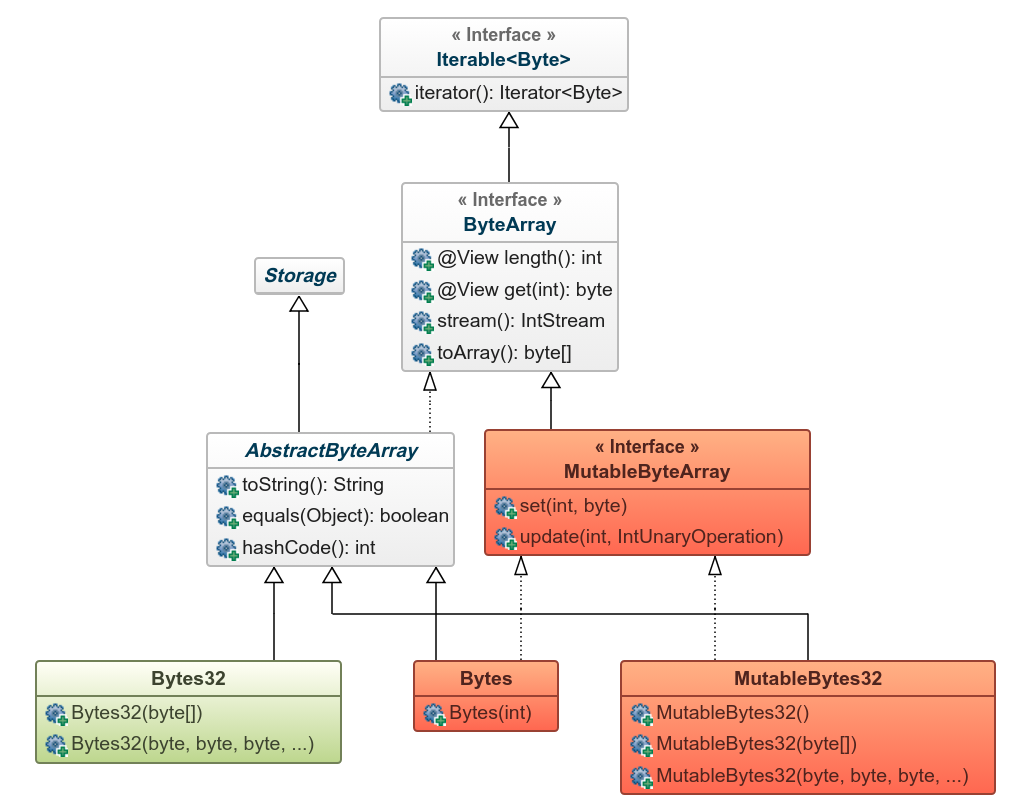
\includegraphics{pics/bytes.png}
\caption{Figure 14. Specialized byte array classes.}
\end{figure}

Figure 14 shows the hierarchy of the specialized classes for arrays of
bytes, available in Takamaka. The interface
\texttt{StorageByteArrayView} defines the methods that read data from an
array of bytes, while the interface \texttt{StorageByteArray} defines
the modification methods. Class \texttt{StorageTreeByteArray} allows one
to create byte arrays of any length, specified at construction time.
Classes \texttt{Bytes32} and \texttt{Bytes32Snapshot} have, instead,
fixed length of 32 bytes; their constructors include one that allows one
to specify such 32 bytes, which is useful for calling the constructor
from outside the blockchain, since \texttt{byte} is a storage type.
While a \texttt{Bytes32} is modifiable, instances of class
\texttt{Bytes32Snapshot} are not modifiable after being created and are
\texttt{@Exported}. There are sibling classes for different, fixed
sizes, such as \texttt{Bytes64} and \texttt{Bytes8Snaphot}. For a full
description of the methods of these classes and interfaces, we refer to
their JavaDoc.

\hypertarget{storage-maps}{%
\section{Storage Maps }\label{storage-maps}}

Maps are dynamic associations of objects to objects. They are useful for
programming smart contracts, as their extensive use in Solidity proves.
However, most such uses are related to the withdrawal pattern, that is
not needed in Takamaka. Nevertheless, there are still situations when
maps are useful in Takamaka code, as we show below.

Java has many implementations of maps, that can be used in Takamaka.
However, they are not storage objects and consequently cannot be stored
in a Hotmoka node. This section describes the
\texttt{io.takamaka.code.util.StorageTreeMap\textless{}K,V\textgreater{}}
class, that extends \texttt{Storage} and whose instances can then be
held in the store of a node, if keys \texttt{K} and values \texttt{V}
can be stored in a node as well.

We refer to the JavaDoc of \texttt{StorageTreeMap} for a full
description of its methods, that are similar to those of traditional
Java maps. Here, we just observe that a key is mapped into a value by
calling method \texttt{void\ put(K\ key,\ V\ value)}, while the value
bound to a key is retrieved by calling \texttt{V\ get(Object\ key)}. It
is possible to yield a default value when a key is not in the map, by
calling \texttt{V\ getOrDefault(Object\ key,\ V\ \_default)} or its
sibling
\texttt{V\ getOrDefault(Object\ key,\ Supplier\textless{}?\ extends\ V\textgreater{}\ \_default)},
that evaluates the default value only if needed. Method
\texttt{V\ putIfAbsent(K\ key,\ V\ value)}, binds the key to the value
only if the key is unbound. Similarly for its sibling
\texttt{V\ computeIfAbsent(K\ key,\ Supplier\textless{}?\ extends\ V\textgreater{}\ value)}
that, however, evaluates the new value only if needed (these two methods
differ for their returned value, as in Java maps. Please refer to their
JavaDoc).

Instances of \texttt{StorageTreeMap\textless{}K,V\textgreater{}} keep
keys in increasing order. Namely, if type \texttt{K} has a natural
order, that order is used. Otherwise, keys (that must be storage
objects) are kept ordered by increasing storage reference. Consequently,
methods \texttt{K\ min()} and \texttt{K\ max()} yield the minimal and
the maximal key of a map. Method
\texttt{List\textless{}K\textgreater{}\ keyList()} yields the ordered
list of the keys of a map; method
\texttt{Stream\textless{}K\textgreater{}\ keys()} yields the same, as an
ordered stream; method
\texttt{Stream\textless{}Entry\textless{}K,V\textgreater{}\textgreater{}\ stream()}
yields the ordered stream of the entries (ie., key/value pairs) of a
map. Compare this with Solidity, where maps do not know the set of their
keys.

\begin{figure}
\centering
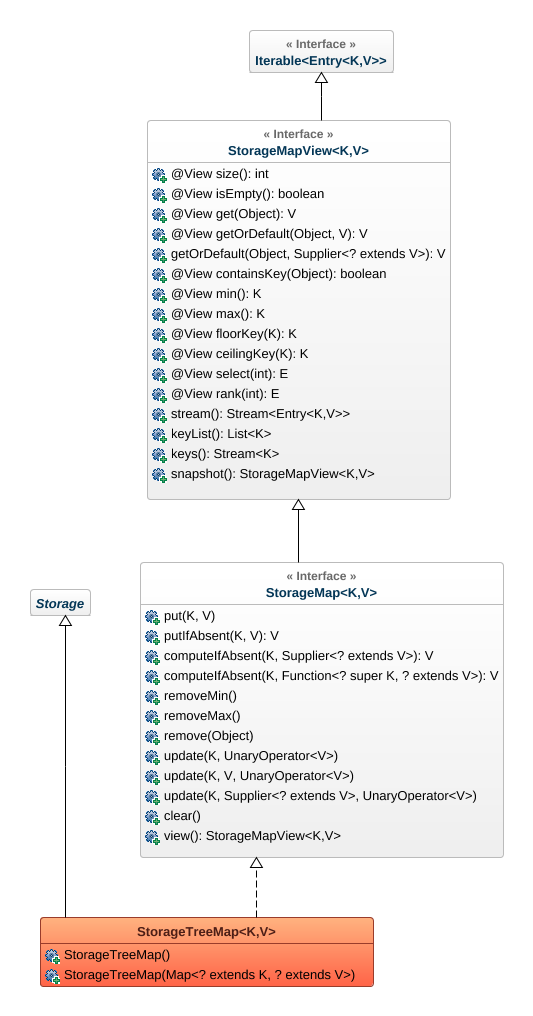
\includegraphics{pics/maps.png}
\caption{Figure 15. The hierarchy of storage maps.}
\end{figure}

Figure 15 shows the hierarchy of the
\texttt{StorageTreeMap\textless{}K,V\textgreater{}} class. It implements
the interface \texttt{StorageMap\textless{}K,V\textgreater{}}, that
defines the methods that modify a map. That interface extends the
interface \texttt{StorageMapView\textless{}K,V\textgreater{}} that,
instead, defines the methods that read data from a map, but do not
modify it. Methods \texttt{snapshot()} and \texttt{view()} return an
\texttt{@Exported} \texttt{StorageMapView\textless{}K,V\textgreater{}},
in constant time.

There are specialized map classes, optimzied for specific kinds of keys,
such as \texttt{StorageTreeIntMap\textless{}V\textgreater{}}, whose keys
are \texttt{int} values. We refer to their JavaDoc for further
information.

\hypertarget{a-blind-auction-contract}{%
\subsection{A Blind Auction Contract }\label{a-blind-auction-contract}}

\textbf{{[}Run \texttt{git\ checkout\ blind\_auction\ -\/-} inside the
\texttt{hotmoka\_tutorial} repository{]}}

This section exemplifies the use of class \texttt{StorageTreeMap} for
writing a smart contract that implements a \emph{blind auction}. That
contract allows a \emph{beneficiary} to sell an item to the buying
contract that offers the highest bid. Since data in blockchain is
public, in a non-blind auction it is possible that bidders eavesdrop the
offers of other bidders in order to place an offer that is only slightly
higher than the current best offer. A blind auction, instead, uses a
two-phases mechanism: in the initial \emph{bidding time}, bidders place
bids, hashed, so that they do not reveal their amount. After the bidding
time expires, the second phase, called \emph{reveal time}, allows
bidders to reveal the real values of their bids and the auction contract
to determine the actual winner. This works since, to reveal a bid, each
bidder provides the real data of the bid. The auction contract then
recomputes the hash from real data and checks if the result matches the
hash provided at bidding time. If not, the bid is considered invalid.
Bidders can even place fake offers on purpose, in order to confuse other
bidders.

Create in Eclipse a new Maven Java 11 (or later) project named
\texttt{auction}. You can do this by duplicating the project
\texttt{family} (make sure to store the project inside the
\texttt{hotmoka} directory, as a sibling of \texttt{family},
\texttt{ponzi}, \texttt{tictactoe} and \texttt{blockchain}). Use the
following \texttt{pom.xml}:

\begin{Shaded}
\begin{Highlighting}[]
\KeywordTok{<project}\OtherTok{ xmlns=}\StringTok{"http://maven.apache.org/POM/4.0.0"}
\OtherTok{    xmlns:xsi=}\StringTok{"http://www.w3.org/2001/XMLSchema-instance"}
\OtherTok{    xsi:schemaLocation=}\StringTok{"http://maven.apache.org/POM/4.0.0}
\StringTok{                        http://maven.apache.org/xsd/maven-4.0.0.xsd"}\KeywordTok{>}

  \KeywordTok{<modelVersion>}\NormalTok{4.0.0}\KeywordTok{</modelVersion>}
  \KeywordTok{<groupId>}\NormalTok{io.hotmoka}\KeywordTok{</groupId>}
  \KeywordTok{<artifactId>}\NormalTok{auction}\KeywordTok{</artifactId>}
  \KeywordTok{<version>}\NormalTok{0.0.1-SNAPSHOT}\KeywordTok{</version>}

  \KeywordTok{<properties>}
    \KeywordTok{<project.build.sourceEncoding>}\NormalTok{UTF-8}\KeywordTok{</project.build.sourceEncoding>}
    \KeywordTok{<maven.compiler.source>}\NormalTok{11}\KeywordTok{</maven.compiler.source>}
    \KeywordTok{<maven.compiler.target>}\NormalTok{11}\KeywordTok{</maven.compiler.target>}
    \KeywordTok{<failOnMissingWebXml>}\NormalTok{false}\KeywordTok{</failOnMissingWebXml>}
  \KeywordTok{</properties>}

  \KeywordTok{<dependencies>}
    \KeywordTok{<dependency>}
      \KeywordTok{<groupId>}\NormalTok{io.hotmoka}\KeywordTok{</groupId>}
      \KeywordTok{<artifactId>}\NormalTok{io-takamaka-code}\KeywordTok{</artifactId>}
      \KeywordTok{<version>}\NormalTok{1.0.0}\KeywordTok{</version>}
    \KeywordTok{</dependency>}
  \KeywordTok{</dependencies>}

  \KeywordTok{<build>}
    \KeywordTok{<plugins>}
      \KeywordTok{<plugin>}
        \KeywordTok{<groupId>}\NormalTok{org.apache.maven.plugins}\KeywordTok{</groupId>}
        \KeywordTok{<artifactId>}\NormalTok{maven-compiler-plugin}\KeywordTok{</artifactId>}
        \KeywordTok{<version>}\NormalTok{3.8.1}\KeywordTok{</version>}
          \KeywordTok{<configuration>}
            \KeywordTok{<release>}\NormalTok{11}\KeywordTok{</release>}
          \KeywordTok{</configuration>}
      \KeywordTok{</plugin>}
    \KeywordTok{</plugins>}
  \KeywordTok{</build>}

\KeywordTok{</project>}
\end{Highlighting}
\end{Shaded}

and the following \texttt{module-info.java}:

\begin{Shaded}
\begin{Highlighting}[]
\NormalTok{module auction \{}
\NormalTok{  requires io.}\FunctionTok{takamaka}\NormalTok{.}\FunctionTok{code}\NormalTok{;}
\NormalTok{\}}
\end{Highlighting}
\end{Shaded}

Create package \texttt{io.takamaka.auction} inside
\texttt{src/main/java} and add the following \texttt{BlindAuction.java}
inside that package. It is a Takamaka contract that implements a blind
auction. Since each bidder may place more bids and since such bids must
be kept in storage until reveal time, this code uses a map from bidders
to lists of bids. This smart contract has been inspired by a similar
Solidity contract \protect\hyperlink{blind-auction}{{[}BlindAuction{]}}.
Please note that this code will not compile yet, since it misses two
classes that we will define in the next section.

\begin{Shaded}
\begin{Highlighting}[]
\KeywordTok{package}\ImportTok{ io.takamaka.auction;}

\KeywordTok{import static}\ImportTok{ io.takamaka.code.lang.Takamaka.event;}
\KeywordTok{import static}\ImportTok{ io.takamaka.code.lang.Takamaka.now;}
\KeywordTok{import static}\ImportTok{ io.takamaka.code.lang.Takamaka.require;}

\KeywordTok{import}\ImportTok{ java.math.BigInteger;}
\KeywordTok{import}\ImportTok{ java.security.MessageDigest;}
\KeywordTok{import}\ImportTok{ java.security.NoSuchAlgorithmException;}
\KeywordTok{import}\ImportTok{ java.util.Arrays;}
\KeywordTok{import}\ImportTok{ java.util.function.Supplier;}

\KeywordTok{import}\ImportTok{ io.takamaka.code.lang.Contract;}
\KeywordTok{import}\ImportTok{ io.takamaka.code.lang.Exported;}
\KeywordTok{import}\ImportTok{ io.takamaka.code.lang.FromContract;}
\KeywordTok{import}\ImportTok{ io.takamaka.code.lang.Payable;}
\KeywordTok{import}\ImportTok{ io.takamaka.code.lang.PayableContract;}
\KeywordTok{import}\ImportTok{ io.takamaka.code.lang.Storage;}
\KeywordTok{import}\ImportTok{ io.takamaka.code.util.Bytes32Snapshot;}
\KeywordTok{import}\ImportTok{ io.takamaka.code.util.StorageLinkedList;}
\KeywordTok{import}\ImportTok{ io.takamaka.code.util.StorageList;}
\KeywordTok{import}\ImportTok{ io.takamaka.code.util.StorageMap;}
\KeywordTok{import}\ImportTok{ io.takamaka.code.util.StorageTreeMap;}

\CommentTok{/**}
 \CommentTok{*}\NormalTok{ A contract for a simple auction}\CommentTok{. }\NormalTok{This class is derived from the Solidity code at}
 \CommentTok{*}\NormalTok{ https}\CommentTok{://}\NormalTok{solidity}\CommentTok{.}\NormalTok{readthedocs}\CommentTok{.}\NormalTok{io}\CommentTok{/}\NormalTok{en}\CommentTok{/}\NormalTok{v0}\CommentTok{.5.9/}\NormalTok{solidity}\CommentTok{-}\NormalTok{by}\CommentTok{-}\NormalTok{example}\CommentTok{.}\NormalTok{html}\CommentTok{#}\NormalTok{id}\CommentTok{2}
 \CommentTok{*}\NormalTok{ In this contract}\CommentTok{,}\NormalTok{ bidders place bids together with a hash}\CommentTok{.}\NormalTok{ At the end of}
 \CommentTok{*}\NormalTok{ the bidding period}\CommentTok{,}\NormalTok{ bidders are expected to reveal if and which of their bids}
 \CommentTok{*}\NormalTok{ were real and their actual value}\CommentTok{.}\NormalTok{ Fake bids are refunded}\CommentTok{.}\NormalTok{ Real bids are compared}
 \CommentTok{*}\NormalTok{ and the bidder with the highest bid wins}\CommentTok{.}
 \CommentTok{*/}
\KeywordTok{public} \KeywordTok{class}\NormalTok{ BlindAuction }\KeywordTok{extends}\NormalTok{ Contract \{}

  \CommentTok{/**}
   \CommentTok{*}\NormalTok{ A bid placed by a bidder}\CommentTok{. }\NormalTok{The deposit has been paid in full}\CommentTok{.}
   \CommentTok{*}\NormalTok{ If}\CommentTok{,}\NormalTok{ later}\CommentTok{,}\NormalTok{ the bid will be revealed as fake}\CommentTok{,}\NormalTok{ then the deposit will}
   \CommentTok{*}\NormalTok{ be fully refunded}\CommentTok{.}\NormalTok{ If}\CommentTok{,}\NormalTok{ instead}\CommentTok{,}\NormalTok{ the bid will be revealed as real}\CommentTok{,}\NormalTok{ but for}
   \CommentTok{*}\NormalTok{ a lower amount}\CommentTok{,}\NormalTok{ then only the difference will be refunded}\CommentTok{.}
   \CommentTok{*/}
  \KeywordTok{private} \DataTypeTok{static} \KeywordTok{class}\NormalTok{ Bid }\KeywordTok{extends}\NormalTok{ Storage \{}

    \CommentTok{/**}
     \CommentTok{*}\NormalTok{ The hash that will be regenerated and compared at reveal time}\CommentTok{.}
     \CommentTok{*/}
    \KeywordTok{private} \DataTypeTok{final}\NormalTok{ Bytes32Snapshot hash;}

    \CommentTok{/**}
      \CommentTok{*}\NormalTok{ The value of the bid}\CommentTok{. }\NormalTok{Its real value might be lower and known}
      \CommentTok{*}\NormalTok{ at real time only}\CommentTok{.}
      \CommentTok{*/}
    \KeywordTok{private} \DataTypeTok{final} \BuiltInTok{BigInteger}\NormalTok{ deposit;}

    \KeywordTok{private} \FunctionTok{Bid}\NormalTok{(Bytes32Snapshot hash, }\BuiltInTok{BigInteger}\NormalTok{ deposit) \{}
      \KeywordTok{this}\NormalTok{.}\FunctionTok{hash}\NormalTok{ = hash;}
      \KeywordTok{this}\NormalTok{.}\FunctionTok{deposit}\NormalTok{ = deposit;}
\NormalTok{    \}}

    \CommentTok{/**}
     \CommentTok{*}\NormalTok{ Recomputes the hash of a bid at reveal time and compares it}
     \CommentTok{*}\NormalTok{ against the hash provided at bidding time}\CommentTok{. }\NormalTok{If they match}\CommentTok{,}
     \CommentTok{*}\NormalTok{ we can reasonably trust the bid}\CommentTok{.}
     \CommentTok{*} 
     \CommentTok{*} \AnnotationTok{@param revealed }\NormalTok{the revealed bid}
     \CommentTok{*} \AnnotationTok{@param digest }\NormalTok{the hasher}
     \CommentTok{*} \AnnotationTok{@return }\NormalTok{true if and only if the hashes match}
     \CommentTok{*/}
    \KeywordTok{private} \DataTypeTok{boolean} \FunctionTok{matches}\NormalTok{(RevealedBid revealed, }\BuiltInTok{MessageDigest}\NormalTok{ digest) \{}
\NormalTok{      digest.}\FunctionTok{update}\NormalTok{(revealed.}\FunctionTok{value}\NormalTok{.}\FunctionTok{toByteArray}\NormalTok{());}
\NormalTok{      digest.}\FunctionTok{update}\NormalTok{(revealed.}\FunctionTok{fake}\NormalTok{ ? (}\DataTypeTok{byte}\NormalTok{) }\DecValTok{0}\NormalTok{ : (}\DataTypeTok{byte}\NormalTok{) }\DecValTok{1}\NormalTok{);}
\NormalTok{      digest.}\FunctionTok{update}\NormalTok{(revealed.}\FunctionTok{salt}\NormalTok{.}\FunctionTok{toArray}\NormalTok{());}
      \KeywordTok{return} \BuiltInTok{Arrays}\NormalTok{.}\FunctionTok{equals}\NormalTok{(hash.}\FunctionTok{toArray}\NormalTok{(), digest.}\FunctionTok{digest}\NormalTok{());}
\NormalTok{    \}}
\NormalTok{  \}}

  \CommentTok{/**}
   \CommentTok{*}\NormalTok{ A bid revealed by a bidder at reveal time}\CommentTok{. }\NormalTok{The bidder shows}
   \CommentTok{*}\NormalTok{ if the corresponding bid was fake or real}\CommentTok{,}\NormalTok{ and how much was the}
   \CommentTok{*}\NormalTok{ actual value of the bid}\CommentTok{.}\NormalTok{ This might be lower than previously communicated}\CommentTok{.}
   \CommentTok{*/}
  \AttributeTok{@Exported}
  \KeywordTok{public} \DataTypeTok{static} \KeywordTok{class}\NormalTok{ RevealedBid }\KeywordTok{extends}\NormalTok{ Storage \{}
    \KeywordTok{private} \DataTypeTok{final} \BuiltInTok{BigInteger}\NormalTok{ value;}
    \KeywordTok{private} \DataTypeTok{final} \DataTypeTok{boolean}\NormalTok{ fake;}

    \CommentTok{/**}
     \CommentTok{*}\NormalTok{ The salt used to strengthen the hashing}\CommentTok{.}
     \CommentTok{*/}
    \KeywordTok{private} \DataTypeTok{final}\NormalTok{ Bytes32Snapshot salt;}

    \KeywordTok{public} \FunctionTok{RevealedBid}\NormalTok{(}\BuiltInTok{BigInteger}\NormalTok{ value, }\DataTypeTok{boolean}\NormalTok{ fake, Bytes32Snapshot salt) \{}
      \KeywordTok{this}\NormalTok{.}\FunctionTok{value}\NormalTok{ = value;}
      \KeywordTok{this}\NormalTok{.}\FunctionTok{fake}\NormalTok{ = fake;}
      \KeywordTok{this}\NormalTok{.}\FunctionTok{salt}\NormalTok{ = salt;}
\NormalTok{    \}}
\NormalTok{  \}}

  \CommentTok{/**}
   \CommentTok{*}\NormalTok{ The beneficiary that}\CommentTok{,}\NormalTok{ at the end of the reveal time}\CommentTok{,}\NormalTok{ will receive the highest bid}\CommentTok{.}
   \CommentTok{*/}
  \KeywordTok{private} \DataTypeTok{final}\NormalTok{ PayableContract beneficiary;}

  \CommentTok{/**}
   \CommentTok{*}\NormalTok{ The bids for each bidder}\CommentTok{. }\NormalTok{A bidder might place more bids}\CommentTok{.}
   \CommentTok{*/}
  \KeywordTok{private} \DataTypeTok{final}\NormalTok{ StorageMap<PayableContract, StorageList<Bid>> bids = }\KeywordTok{new}\NormalTok{ StorageTreeMap<>();}

  \CommentTok{/**}
   \CommentTok{*}\NormalTok{ The time when the bidding time ends}\CommentTok{.}
   \CommentTok{*/}
  \KeywordTok{private} \DataTypeTok{final} \DataTypeTok{long}\NormalTok{ biddingEnd;}

  \CommentTok{/**}
   \CommentTok{*}\NormalTok{ The time when the reveal time ends}\CommentTok{.}
   \CommentTok{*/}
  \KeywordTok{private} \DataTypeTok{final} \DataTypeTok{long}\NormalTok{ revealEnd;}

  \CommentTok{/**}
   \CommentTok{*}\NormalTok{ The bidder with the highest bid}\CommentTok{,}\NormalTok{ at reveal time}\CommentTok{.}
   \CommentTok{*/}
  \KeywordTok{private}\NormalTok{ PayableContract highestBidder;}

  \CommentTok{/**}
   \CommentTok{*}\NormalTok{ The highest bid}\CommentTok{,}\NormalTok{ at reveal time}\CommentTok{.}
   \CommentTok{*/}
  \KeywordTok{private} \BuiltInTok{BigInteger}\NormalTok{ highestBid;}

  \CommentTok{/**}
   \CommentTok{*}\NormalTok{ Creates a blind auction contract}\CommentTok{.}
   \CommentTok{*} 
   \CommentTok{*} \AnnotationTok{@param biddingTime }\NormalTok{the length of the bidding time}
   \CommentTok{*} \AnnotationTok{@param revealTime }\NormalTok{the length of the reveal time}
   \CommentTok{*/}
  \KeywordTok{public} \AttributeTok{@FromContract}\NormalTok{(PayableContract.}\FunctionTok{class}\NormalTok{) }\FunctionTok{BlindAuction}\NormalTok{(}\DataTypeTok{int}\NormalTok{ biddingTime, }\DataTypeTok{int}\NormalTok{ revealTime) \{}
    \FunctionTok{require}\NormalTok{(biddingTime > }\DecValTok{0}\NormalTok{, }\StringTok{"Bidding time must be positive"}\NormalTok{);}
    \FunctionTok{require}\NormalTok{(revealTime > }\DecValTok{0}\NormalTok{, }\StringTok{"Reveal time must be positive"}\NormalTok{);}

    \KeywordTok{this}\NormalTok{.}\FunctionTok{beneficiary}\NormalTok{ = (PayableContract) }\FunctionTok{caller}\NormalTok{();}
    \KeywordTok{this}\NormalTok{.}\FunctionTok{biddingEnd}\NormalTok{ = }\FunctionTok{now}\NormalTok{() + biddingTime;}
    \KeywordTok{this}\NormalTok{.}\FunctionTok{revealEnd}\NormalTok{ = biddingEnd + revealTime;}
\NormalTok{  \}}

  \CommentTok{/**}
   \CommentTok{*}\NormalTok{ Places a blinded bid with the given hash}\CommentTok{.}
   \CommentTok{*}\NormalTok{ The money sent is only refunded if the bid is correctly}
   \CommentTok{*}\NormalTok{ revealed in the revealing phase}\CommentTok{.}\NormalTok{ The bid is valid if the}
   \CommentTok{*}\NormalTok{ money sent together with the bid is at least }\CommentTok{"}\NormalTok{value}\CommentTok{"}\NormalTok{ and}
   \CommentTok{*} \CommentTok{"}\NormalTok{fake}\CommentTok{"}\NormalTok{ is not true}\CommentTok{.}\NormalTok{ Setting }\CommentTok{"}\NormalTok{fake}\CommentTok{"}\NormalTok{ to true and sending}
   \CommentTok{*}\NormalTok{ not the exact amount are ways to hide the real bid but}
   \CommentTok{*}\NormalTok{ still make the required deposit}\CommentTok{.}\NormalTok{ The same bidder can place multiple bids}\CommentTok{.}
   \CommentTok{*/}
  \KeywordTok{public} \AttributeTok{@Payable} \AttributeTok{@FromContract}\NormalTok{(PayableContract.}\FunctionTok{class}\NormalTok{) }\DataTypeTok{void}\NormalTok{ bid}
\NormalTok{      (}\BuiltInTok{BigInteger}\NormalTok{ amount, Bytes32Snapshot hash) \{}

    \FunctionTok{onlyBefore}\NormalTok{(biddingEnd);}
\NormalTok{    bids.}\FunctionTok{computeIfAbsent}\NormalTok{((PayableContract) }\FunctionTok{caller}\NormalTok{(), (Supplier<StorageList<Bid>>) StorageLinkedList::}\KeywordTok{new}\NormalTok{)}
\NormalTok{      .}\FunctionTok{add}\NormalTok{(}\KeywordTok{new} \FunctionTok{Bid}\NormalTok{(hash, amount));}
\NormalTok{  \}}

  \CommentTok{/**}
   \CommentTok{*}\NormalTok{ Reveals a bid of the caller}\CommentTok{. }\NormalTok{The caller will get a refund for all correctly}
   \CommentTok{*}\NormalTok{ blinded invalid bids and for all bids except for the totally highest}\CommentTok{.}
   \CommentTok{*} 
   \CommentTok{*} \AnnotationTok{@param revealed }\NormalTok{the revealed bid}
   \CommentTok{*} \AnnotationTok{@throws NoSuchAlgorithmException }\NormalTok{if the hashing algorithm is not available}
   \CommentTok{*/}
  \KeywordTok{public} \AttributeTok{@FromContract}\NormalTok{(PayableContract.}\FunctionTok{class}\NormalTok{) }\DataTypeTok{void}\NormalTok{ reveal}
\NormalTok{      (RevealedBid revealed) }\KeywordTok{throws} \BuiltInTok{NoSuchAlgorithmException}\NormalTok{ \{}

    \FunctionTok{onlyAfter}\NormalTok{(biddingEnd);}
    \FunctionTok{onlyBefore}\NormalTok{(revealEnd);}
\NormalTok{    PayableContract bidder = (PayableContract) }\FunctionTok{caller}\NormalTok{();}
\NormalTok{    StorageList<Bid> bids = }\KeywordTok{this}\NormalTok{.}\FunctionTok{bids}\NormalTok{.}\FunctionTok{get}\NormalTok{(bidder);}
    \FunctionTok{require}\NormalTok{(bids != }\KeywordTok{null}\NormalTok{ && bids.}\FunctionTok{size}\NormalTok{() > }\DecValTok{0}\NormalTok{, }\StringTok{"No bids to reveal"}\NormalTok{);}
    \FunctionTok{require}\NormalTok{(revealed != }\KeywordTok{null}\NormalTok{, () -> }\StringTok{"The revealed bid cannot be null"}\NormalTok{);}

    \CommentTok{// any other hashing algorithm will do, as long as}
    \CommentTok{// both bidder and auction contract use the same}
    \BuiltInTok{MessageDigest}\NormalTok{ digest = }\BuiltInTok{MessageDigest}\NormalTok{.}\FunctionTok{getInstance}\NormalTok{(}\StringTok{"SHA-256"}\NormalTok{);}
    \CommentTok{// by removing the head of the list, it makes it impossible}
    \CommentTok{// for the caller to re-claim the same deposits}
\NormalTok{    bidder.}\FunctionTok{receive}\NormalTok{(}\FunctionTok{refundFor}\NormalTok{(bidder, bids.}\FunctionTok{removeFirst}\NormalTok{(), revealed, digest));}
\NormalTok{  \}}

  \CommentTok{/**}
   \CommentTok{*}\NormalTok{ Ends the auction and sends the highest bid to the beneficiary}\CommentTok{.}
   \CommentTok{*} 
   \CommentTok{*} \AnnotationTok{@return }\NormalTok{the highest bidder}
   \CommentTok{*/}
  \KeywordTok{public}\NormalTok{ PayableContract }\FunctionTok{auctionEnd}\NormalTok{() \{}
    \FunctionTok{onlyAfter}\NormalTok{(revealEnd);}
\NormalTok{    PayableContract winner = highestBidder;}
        
    \KeywordTok{if}\NormalTok{ (winner != }\KeywordTok{null}\NormalTok{) \{}
\NormalTok{      beneficiary.}\FunctionTok{receive}\NormalTok{(highestBid);}
      \FunctionTok{event}\NormalTok{(}\KeywordTok{new} \FunctionTok{AuctionEnd}\NormalTok{(winner, highestBid));}
\NormalTok{      highestBidder = }\KeywordTok{null}\NormalTok{;}
\NormalTok{    \}}

    \KeywordTok{return}\NormalTok{ winner;}
\NormalTok{  \}}

  \CommentTok{/**}
   \CommentTok{*}\NormalTok{ Checks how much of the deposit should be refunded for a given bid}\CommentTok{.}
   \CommentTok{*} 
   \CommentTok{*} \AnnotationTok{@param bidder }\NormalTok{the bidder that placed the bid}
   \CommentTok{*} \AnnotationTok{@param bid }\NormalTok{the bid}\CommentTok{,}\NormalTok{ as was placed at bidding time}
   \CommentTok{*} \AnnotationTok{@param revealed }\NormalTok{the bid}\CommentTok{,}\NormalTok{ as was revealed later}
   \CommentTok{*} \AnnotationTok{@param digest }\NormalTok{the hashing algorithm}
   \CommentTok{*} \AnnotationTok{@return }\NormalTok{the amount to refund}
   \CommentTok{*/}
  \KeywordTok{private} \BuiltInTok{BigInteger} \FunctionTok{refundFor}\NormalTok{(PayableContract bidder, Bid bid,}
\NormalTok{      RevealedBid revealed, }\BuiltInTok{MessageDigest}\NormalTok{ digest) \{}

    \KeywordTok{if}\NormalTok{ (!bid.}\FunctionTok{matches}\NormalTok{(revealed, digest))}
      \CommentTok{// the bid was not actually revealed: no refund}
      \KeywordTok{return} \BuiltInTok{BigInteger}\NormalTok{.}\FunctionTok{ZERO}\NormalTok{;}
    \KeywordTok{else} \KeywordTok{if}\NormalTok{ (!revealed.}\FunctionTok{fake}\NormalTok{ && bid.}\FunctionTok{deposit}\NormalTok{.}\FunctionTok{compareTo}\NormalTok{(revealed.}\FunctionTok{value}\NormalTok{) >= }\DecValTok{0}
\NormalTok{        && }\FunctionTok{placeBid}\NormalTok{(bidder, revealed.}\FunctionTok{value}\NormalTok{))}
      \CommentTok{// the bid was correctly revealed and is the best up to now:}
      \CommentTok{// only the difference between promised and provided is refunded;}
      \CommentTok{// the rest might be refunded later if a better bid will be revealed}
      \KeywordTok{return}\NormalTok{ bid.}\FunctionTok{deposit}\NormalTok{.}\FunctionTok{subtract}\NormalTok{(revealed.}\FunctionTok{value}\NormalTok{);}
    \KeywordTok{else}
      \CommentTok{// the bid was correctly revealed and is not the best one:}
      \CommentTok{// it is fully refunded}
      \KeywordTok{return}\NormalTok{ bid.}\FunctionTok{deposit}\NormalTok{;}
\NormalTok{  \}}

  \CommentTok{/**}
   \CommentTok{*}\NormalTok{ Takes note that a bidder has correctly revealed a bid for the given value}\CommentTok{.}
   \CommentTok{*} 
   \CommentTok{*} \AnnotationTok{@param bidder }\NormalTok{the bidder}
   \CommentTok{*} \AnnotationTok{@param value }\NormalTok{the value}\CommentTok{,}\NormalTok{ as revealed}
   \CommentTok{*} \AnnotationTok{@return }\NormalTok{true if and only if this is the best bid}\CommentTok{,}\NormalTok{ up to now}
   \CommentTok{*/}
  \KeywordTok{private} \DataTypeTok{boolean} \FunctionTok{placeBid}\NormalTok{(PayableContract bidder, }\BuiltInTok{BigInteger}\NormalTok{ value) \{}
    \KeywordTok{if}\NormalTok{ (highestBid != }\KeywordTok{null}\NormalTok{ && value.}\FunctionTok{compareTo}\NormalTok{(highestBid) <= }\DecValTok{0}\NormalTok{)}
      \CommentTok{// this is not the best bid seen so far}
      \KeywordTok{return} \KeywordTok{false}\NormalTok{;}

    \CommentTok{// if there was a best bidder already, its bid is refunded}
    \KeywordTok{if}\NormalTok{ (highestBidder != }\KeywordTok{null}\NormalTok{)}
      \CommentTok{// Refund the previously highest bidder}
\NormalTok{      highestBidder.}\FunctionTok{receive}\NormalTok{(highestBid);}

    \CommentTok{// take note that this is the best bid up to now}
\NormalTok{    highestBid = value;}
\NormalTok{    highestBidder = bidder;}
    \FunctionTok{event}\NormalTok{(}\KeywordTok{new} \FunctionTok{BidIncrease}\NormalTok{(bidder, value));}

    \KeywordTok{return} \KeywordTok{true}\NormalTok{;}
\NormalTok{  \}}

  \KeywordTok{private} \DataTypeTok{static} \DataTypeTok{void} \FunctionTok{onlyBefore}\NormalTok{(}\DataTypeTok{long}\NormalTok{ when) \{}
    \FunctionTok{require}\NormalTok{(}\FunctionTok{now}\NormalTok{() < when, }\StringTok{"Too late"}\NormalTok{);}
\NormalTok{  \}}

  \KeywordTok{private} \DataTypeTok{static} \DataTypeTok{void} \FunctionTok{onlyAfter}\NormalTok{(}\DataTypeTok{long}\NormalTok{ when) \{}
    \FunctionTok{require}\NormalTok{(}\FunctionTok{now}\NormalTok{() > when, }\StringTok{"Too early"}\NormalTok{);}
\NormalTok{  \}}
\NormalTok{\}}
\end{Highlighting}
\end{Shaded}

Let us discuss this (long) code, starting from the inner classes.

Class \texttt{Bid} represents a bid placed by a contract that takes part
to the auction. This information will be stored in blockchain at bidding
time, hence it is known to all other participants. An instance of
\texttt{Bid} contains the \texttt{deposit} paid at time of placing the
bid. This is not necessarily the real value of the offer but must be at
least as large as the real offer, or otherwise the bid will be
considered as invalid at reveal time. Instances of \texttt{Bid} contain
a \texttt{hash} consisting of 32 bytes. As already said, this will be
recomputed at reveal time and matched against the result. Since arrays
cannot be stored in blockchain, we use storage class
\texttt{io.takamaka.code.util.Bytes32Snapshot} here, a library class
that holds 32 bytes, as a traditional array (see
\protect\hyperlink{specialized-storage-array-classes}{Specialized
Storage Array Classes}). It is well possible to use a
\texttt{StorageArray} of a wrapper of \texttt{byte} here, but
\texttt{Bytes32Snapshot} is much more compact and its methods consume
less gas.

Class \texttt{RevealedBid} describes a bid revealed after bidding time.
It contains the real value of the bid, the salt used to strengthen the
hashing algorithm and a boolean \texttt{fake} that, when true, means
that the bid must be considered as invalid, since it was only placed in
order to confuse other bidders. It is possible to recompute and check
the hash of a revealed bid through method \texttt{Bid.matches()}, that
uses a given hashing algorithm (\texttt{digest}, a Java
\texttt{java.security.MessageDigest}) to hash value, fake mark and salt
into bytes, finally compared against the hash provided at bidding time.

The \texttt{BlindAuction} contract stores the \texttt{beneficiary} of
the auction. It is the contract that created the contract and is
consequently initialized, in the constructor of \texttt{BlindAuction},
to its caller. The constructor must annotated as \texttt{@FromContract}
because of that. The same constructor receives the length of bidding
time and reveal time, in milliseconds. This allows the contract to
compute tha absolute ending time for the bidding phase and for the
reveal phase, stored into fields \texttt{biddingEnd} and
\texttt{revealEnd}, respectively. Note, in the contructor of
\texttt{BlindAuction}, the use of the static method
\texttt{io.takamaka.code.lang.Takamaka.now()}, that yields the current
time, as with the traditional \texttt{System.currentTimeMillis()} of
Java (that instead cannot be used in Takamaka code). Method
\texttt{now()}, in a blockchain, yields the time of creation of the
block of the current transaction, as seen by its miner. That time is
reported in the block and hence is independent from the machine that
runs the contract, which guarantees determinism.

Method \texttt{bid()} allows a caller (the bidder) to place a bid during
the bidding phase. An instance of \texttt{Bid} is created and added to a
list, specific to each bidder. Here is where our map comes to help.
Namely, field \texttt{bids} holds a
\texttt{StorageTreeMap\textless{}PayableContract,\ StorageList\textless{}Bid\textgreater{}\textgreater{}},
that can be held in blockchain since it is a storage map between storage
keys and storage values. Method \texttt{bid()} computes an empty list of
bids if it is the first time that a bidder places a bid. For that, it
uses method \texttt{computeIfAbsent()} of \texttt{StorageMap}. If it
used method \texttt{get()}, it would run into a null-pointer exception
the first time a bidder places a bid. That is, storage maps default to
\texttt{null}, as all Java maps, but differently to Solidity maps, that
provide a new value automatically when undefined.

Method \texttt{reveal()} is called by each bidder during the reveal
phase. It accesses the \texttt{bids} placed by the bidder during the
bidding time. The method matches each revealed bid against the
corresponding list of bids for the player, by calling method
\texttt{refundFor()}, that determines how much of the deposit must be
refunded to the bidder. Namely, if a bid was fake or was not the best
bid, it must be refunded entirely. If it was the best bid, it must be
partially refunded if the apparent \texttt{deposit} turns out to be
higher than the actual value of the revealed bid. While bids are
refunded, method \texttt{placeBid} updates the best bid information.

Method \texttt{auctionEnd()} is meant to be called after the reveal
phase. If there is a winner, it sends the highest bid to the
beneficiary.

Note the use of methods \texttt{onlyBefore()} and \texttt{onlyAfter()}
to guarantee that some methods are only run at the right moment.

\hypertarget{events}{%
\subsection{Events }\label{events}}

\textbf{{[}Run \texttt{git\ checkout\ blind\_auction\_events\ -\/-}
inside the \texttt{hotmoka\_tutorial} repository{]}}

The code in the previous section does not compile since it misses two
classes \texttt{BidIncrease.java} and \texttt{AuctionEnd.java}, that we
report below. Namely, the code of the blind auction contract contains
some lines that generate \emph{events}, such as:

\begin{Shaded}
\begin{Highlighting}[]
\FunctionTok{event}\NormalTok{(}\KeywordTok{new} \FunctionTok{AuctionEnd}\NormalTok{(winner, highestBid));}
\end{Highlighting}
\end{Shaded}

Events are milestones that are saved in the store of a Hotmoka node.
From outside the node, it is possible to subscribe to specific events
and get notified as soon as an event of that kind occurs, to trigger
actions when that happens. In terms of the Takamaka language, events are
generated through the
\texttt{io.takamaka.code.lang.Takamaka.event(Event\ event)} method, that
receives a parameter of type \texttt{io.takamaka.code.lang.Event}. The
latter is simply an abstract class that extends \texttt{Storage}. Hence,
events will be stored in the node as part of the transaction that
generated that event. The constructor of class \texttt{Event} is
annotated as \texttt{FromContract}, which allows to create events from
the code of contracts only. The creating contract is available through
method \texttt{creator()} of class \texttt{Event}.

In our example, the \texttt{BlindAuction} class uses two events, that
you can add to the \texttt{io.takamaka.auction} package and are defined
as follows:

\begin{Shaded}
\begin{Highlighting}[]
\KeywordTok{package}\ImportTok{ io.takamaka.auction;}

\KeywordTok{import}\ImportTok{ java.math.BigInteger;}

\KeywordTok{import}\ImportTok{ io.takamaka.code.lang.FromContract;}
\KeywordTok{import}\ImportTok{ io.takamaka.code.lang.Event;}
\KeywordTok{import}\ImportTok{ io.takamaka.code.lang.PayableContract;}
\KeywordTok{import}\ImportTok{ io.takamaka.code.lang.View;}

\KeywordTok{public} \KeywordTok{class}\NormalTok{ BidIncrease }\KeywordTok{extends} \BuiltInTok{Event}\NormalTok{ \{}
  \KeywordTok{public} \DataTypeTok{final}\NormalTok{ PayableContract bidder;}
  \KeywordTok{public} \DataTypeTok{final} \BuiltInTok{BigInteger}\NormalTok{ amount;}

  \AttributeTok{@FromContract} \FunctionTok{BidIncrease}\NormalTok{(PayableContract bidder, }\BuiltInTok{BigInteger}\NormalTok{ amount) \{}
    \KeywordTok{this}\NormalTok{.}\FunctionTok{bidder}\NormalTok{ = bidder;}
    \KeywordTok{this}\NormalTok{.}\FunctionTok{amount}\NormalTok{ = amount;}
\NormalTok{  \}}

  \KeywordTok{public} \AttributeTok{@View}\NormalTok{ PayableContract }\FunctionTok{getBidder}\NormalTok{() \{}
    \KeywordTok{return}\NormalTok{ bidder;}
\NormalTok{  \}}

  \KeywordTok{public} \AttributeTok{@View} \BuiltInTok{BigInteger} \FunctionTok{getAmount}\NormalTok{() \{}
    \KeywordTok{return}\NormalTok{ amount;}
\NormalTok{  \}}
\NormalTok{\}}
\end{Highlighting}
\end{Shaded}

and

\begin{Shaded}
\begin{Highlighting}[]
\KeywordTok{package}\ImportTok{ io.takamaka.auction;}

\KeywordTok{import}\ImportTok{ java.math.BigInteger;}

\KeywordTok{import}\ImportTok{ io.takamaka.code.lang.FromContract;}
\KeywordTok{import}\ImportTok{ io.takamaka.code.lang.Event;}
\KeywordTok{import}\ImportTok{ io.takamaka.code.lang.PayableContract;}
\KeywordTok{import}\ImportTok{ io.takamaka.code.lang.View;}

\KeywordTok{public} \KeywordTok{class}\NormalTok{ AuctionEnd }\KeywordTok{extends} \BuiltInTok{Event}\NormalTok{ \{}
  \KeywordTok{public} \DataTypeTok{final}\NormalTok{ PayableContract highestBidder;}
  \KeywordTok{public} \DataTypeTok{final} \BuiltInTok{BigInteger}\NormalTok{ highestBid;}

  \AttributeTok{@FromContract} \FunctionTok{AuctionEnd}\NormalTok{(PayableContract highestBidder, }\BuiltInTok{BigInteger}\NormalTok{ highestBid) \{}
    \KeywordTok{this}\NormalTok{.}\FunctionTok{highestBidder}\NormalTok{ = highestBidder;}
    \KeywordTok{this}\NormalTok{.}\FunctionTok{highestBid}\NormalTok{ = highestBid;}
\NormalTok{  \}}

  \KeywordTok{public} \AttributeTok{@View}\NormalTok{ PayableContract }\FunctionTok{getHighestBidder}\NormalTok{() \{}
    \KeywordTok{return}\NormalTok{ highestBidder;}
\NormalTok{  \}}

  \KeywordTok{public} \AttributeTok{@View} \BuiltInTok{BigInteger} \FunctionTok{getHighestBid}\NormalTok{() \{}
  \KeywordTok{return}\NormalTok{ highestBid;}
\NormalTok{  \}}
\NormalTok{\}}
\end{Highlighting}
\end{Shaded}

Now that all classes have been completed, the project should compile. Go
inside the \texttt{auction} project and run \texttt{mvn\ package}. A
file \texttt{auction-0.0.1-SNAPSHOT.jar} should appear inside
\texttt{target}.

\hypertarget{running-the-blind-auction-contract}{%
\subsection{Running the Blind Auction Contract
}\label{running-the-blind-auction-contract}}

\textbf{{[}Run \texttt{git\ checkout\ blind\_auction\_run\ -\/-} inside
the \texttt{hotmoka\_tutorial} repository{]}}

Go to the \texttt{blockchain} Eclipse project and create a new
\texttt{io.takamaka.auction} package inside \texttt{src/main/java}. Add
the following \texttt{Main.java} class inside that package:

\begin{Shaded}
\begin{Highlighting}[]
\KeywordTok{package}\ImportTok{ io.takamaka.auction;}

\KeywordTok{import static}\ImportTok{ io.hotmoka.beans.types.BasicTypes.BOOLEAN;}
\KeywordTok{import static}\ImportTok{ io.hotmoka.beans.types.BasicTypes.BYTE;}
\KeywordTok{import static}\ImportTok{ io.hotmoka.beans.types.BasicTypes.INT;}
\KeywordTok{import static}\ImportTok{ io.hotmoka.beans.types.ClassType.BIG_INTEGER;}
\KeywordTok{import static}\ImportTok{ io.hotmoka.beans.types.ClassType.BYTES32_SNAPSHOT;}
\KeywordTok{import static}\ImportTok{ io.hotmoka.beans.types.ClassType.PAYABLE_CONTRACT;}
\KeywordTok{import static}\ImportTok{ java.math.BigInteger.ONE;}
\KeywordTok{import static}\ImportTok{ java.math.BigInteger.ZERO;}

\KeywordTok{import}\ImportTok{ java.math.BigInteger;}
\KeywordTok{import}\ImportTok{ java.nio.file.Path;}
\KeywordTok{import}\ImportTok{ java.nio.file.Paths;}
\KeywordTok{import}\ImportTok{ java.security.MessageDigest;}
\KeywordTok{import}\ImportTok{ java.util.ArrayList;}
\KeywordTok{import}\ImportTok{ java.util.Iterator;}
\KeywordTok{import}\ImportTok{ java.util.List;}
\KeywordTok{import}\ImportTok{ java.util.Random;}

\KeywordTok{import}\ImportTok{ io.hotmoka.beans.references.TransactionReference;}
\KeywordTok{import}\ImportTok{ io.hotmoka.beans.requests.ConstructorCallTransactionRequest;}
\KeywordTok{import}\ImportTok{ io.hotmoka.beans.requests.InstanceMethodCallTransactionRequest;}
\KeywordTok{import}\ImportTok{ io.hotmoka.beans.requests.SignedTransactionRequest;}
\KeywordTok{import}\ImportTok{ io.hotmoka.beans.requests.SignedTransactionRequest.Signer;}
\KeywordTok{import}\ImportTok{ io.hotmoka.beans.signatures.ConstructorSignature;}
\KeywordTok{import}\ImportTok{ io.hotmoka.beans.signatures.MethodSignature;}
\KeywordTok{import}\ImportTok{ io.hotmoka.beans.signatures.NonVoidMethodSignature;}
\KeywordTok{import}\ImportTok{ io.hotmoka.beans.signatures.VoidMethodSignature;}
\KeywordTok{import}\ImportTok{ io.hotmoka.beans.types.ClassType;}
\KeywordTok{import}\ImportTok{ io.hotmoka.beans.values.BigIntegerValue;}
\KeywordTok{import}\ImportTok{ io.hotmoka.beans.values.BooleanValue;}
\KeywordTok{import}\ImportTok{ io.hotmoka.beans.values.ByteValue;}
\KeywordTok{import}\ImportTok{ io.hotmoka.beans.values.IntValue;}
\KeywordTok{import}\ImportTok{ io.hotmoka.beans.values.StorageReference;}
\KeywordTok{import}\ImportTok{ io.hotmoka.beans.values.StorageValue;}
\KeywordTok{import}\ImportTok{ io.hotmoka.crypto.SignatureAlgorithm;}
\KeywordTok{import}\ImportTok{ io.hotmoka.memory.MemoryBlockchain;}
\KeywordTok{import}\ImportTok{ io.hotmoka.memory.MemoryBlockchainConfig;}
\KeywordTok{import}\ImportTok{ io.hotmoka.nodes.Node;}
\KeywordTok{import}\ImportTok{ io.hotmoka.nodes.views.InitializedNode;}
\KeywordTok{import}\ImportTok{ io.hotmoka.nodes.views.NodeWithAccounts;}
\KeywordTok{import}\ImportTok{ io.hotmoka.nodes.views.NodeWithJars;}

\KeywordTok{public} \KeywordTok{class}\NormalTok{ Main \{}
  \KeywordTok{public} \DataTypeTok{final} \DataTypeTok{static} \DataTypeTok{int}\NormalTok{ NUM_BIDS = }\DecValTok{40}\NormalTok{; }\CommentTok{// number of bids placed}
  \KeywordTok{public} \DataTypeTok{final} \DataTypeTok{static} \DataTypeTok{int}\NormalTok{ BIDDING_TIME = }\DecValTok{40_000}\NormalTok{; }\CommentTok{// in milliseconds}
  \KeywordTok{public} \DataTypeTok{final} \DataTypeTok{static} \DataTypeTok{int}\NormalTok{ REVEAL_TIME = }\DecValTok{70_000}\NormalTok{; }\CommentTok{// in milliseconds}

  \KeywordTok{public} \DataTypeTok{final} \DataTypeTok{static} \BuiltInTok{BigInteger}\NormalTok{ GREEN_AMOUNT = }\BuiltInTok{BigInteger}\NormalTok{.}\FunctionTok{valueOf}\NormalTok{(}\DecValTok{100_000_000}\NormalTok{);}
  \KeywordTok{public} \DataTypeTok{final} \DataTypeTok{static} \BuiltInTok{BigInteger}\NormalTok{ RED_AMOUNT = ZERO;}
  \KeywordTok{private} \DataTypeTok{final} \DataTypeTok{static} \BuiltInTok{BigInteger}\NormalTok{ _}\DecValTok{100_000}\NormalTok{ = }\BuiltInTok{BigInteger}\NormalTok{.}\FunctionTok{valueOf}\NormalTok{(}\DecValTok{100_000}\NormalTok{);}
  \KeywordTok{private} \DataTypeTok{final} \DataTypeTok{static} \BuiltInTok{BigInteger}\NormalTok{ _}\DecValTok{10_000_000}\NormalTok{ = }\BuiltInTok{BigInteger}\NormalTok{.}\FunctionTok{valueOf}\NormalTok{(}\DecValTok{10_000_000}\NormalTok{);}

  \CommentTok{// useful constants that refer to classes, constructors or methods}
  \KeywordTok{private} \DataTypeTok{final} \DataTypeTok{static}\NormalTok{ ClassType BLIND_AUCTION}
\NormalTok{    = }\KeywordTok{new} \FunctionTok{ClassType}\NormalTok{(}\StringTok{"io.takamaka.auction.BlindAuction"}\NormalTok{);}
  \KeywordTok{private} \DataTypeTok{final} \DataTypeTok{static}\NormalTok{ ConstructorSignature CONSTRUCTOR_BLIND_AUCTION}
\NormalTok{    = }\KeywordTok{new} \FunctionTok{ConstructorSignature}\NormalTok{(BLIND_AUCTION, INT, INT);}
  \KeywordTok{private} \DataTypeTok{final} \DataTypeTok{static}\NormalTok{ ConstructorSignature CONSTRUCTOR_BYTES32_SNAPSHOT}
\NormalTok{    = }\KeywordTok{new} \FunctionTok{ConstructorSignature}\NormalTok{(BYTES32_SNAPSHOT,}
\NormalTok{     BYTE, BYTE, BYTE, BYTE, BYTE, BYTE, BYTE, BYTE,}
\NormalTok{     BYTE, BYTE, BYTE, BYTE, BYTE, BYTE, BYTE, BYTE,}
\NormalTok{     BYTE, BYTE, BYTE, BYTE, BYTE, BYTE, BYTE, BYTE,}
\NormalTok{     BYTE, BYTE, BYTE, BYTE, BYTE, BYTE, BYTE, BYTE);}
  \KeywordTok{private} \DataTypeTok{final} \DataTypeTok{static}\NormalTok{ ConstructorSignature CONSTRUCTOR_REVEALED_BID}
\NormalTok{    = }\KeywordTok{new} \FunctionTok{ConstructorSignature}\NormalTok{(}
        \KeywordTok{new} \FunctionTok{ClassType}\NormalTok{(}\StringTok{"io.takamaka.auction.BlindAuction$RevealedBid"}\NormalTok{),}
\NormalTok{        BIG_INTEGER, BOOLEAN, BYTES32_SNAPSHOT);}
  \KeywordTok{private} \DataTypeTok{final} \DataTypeTok{static}\NormalTok{ MethodSignature BID = }\KeywordTok{new}\NormalTok{ VoidMethodSignature}
\NormalTok{    (BLIND_AUCTION, }\StringTok{"bid"}\NormalTok{, BIG_INTEGER, BYTES32_SNAPSHOT);}
  \KeywordTok{private} \DataTypeTok{final} \DataTypeTok{static}\NormalTok{ MethodSignature REVEAL = }\KeywordTok{new}\NormalTok{ VoidMethodSignature}
\NormalTok{    (BLIND_AUCTION, }\StringTok{"reveal"}\NormalTok{, }\KeywordTok{new} \FunctionTok{ClassType}\NormalTok{(}\StringTok{"io.takamaka.auction.BlindAuction$RevealedBid"}\NormalTok{));}
  \KeywordTok{private} \DataTypeTok{final} \DataTypeTok{static}\NormalTok{ MethodSignature AUCTION_END = }\KeywordTok{new}\NormalTok{ NonVoidMethodSignature}
\NormalTok{    (BLIND_AUCTION, }\StringTok{"auctionEnd"}\NormalTok{, PAYABLE_CONTRACT);}

  \CommentTok{//the hashing algorithm used to hide the bids}
  \KeywordTok{private} \DataTypeTok{final} \BuiltInTok{MessageDigest}\NormalTok{ digest = }\BuiltInTok{MessageDigest}\NormalTok{.}\FunctionTok{getInstance}\NormalTok{(}\StringTok{"SHA-256"}\NormalTok{);}

  \KeywordTok{private} \DataTypeTok{final} \DataTypeTok{long}\NormalTok{ start;  }\CommentTok{// the time when bids started being placed}
  \KeywordTok{private} \DataTypeTok{final}\NormalTok{ NodeWithAccounts node;}
  \KeywordTok{private} \DataTypeTok{final}\NormalTok{ TransactionReference classpath;}
  \KeywordTok{private} \DataTypeTok{final} \BuiltInTok{Signer}\NormalTok{[] signers = }\KeywordTok{new} \BuiltInTok{Signer}\NormalTok{[}\DecValTok{4}\NormalTok{];}
  \KeywordTok{private} \DataTypeTok{final} \BuiltInTok{BigInteger}\NormalTok{[] nonces = \{ ZERO, ZERO, ZERO, ZERO \};}
  \KeywordTok{private} \DataTypeTok{final}\NormalTok{ StorageReference auction;}
  \KeywordTok{private} \DataTypeTok{final} \BuiltInTok{List}\NormalTok{<BidToReveal> bids = }\KeywordTok{new} \BuiltInTok{ArrayList}\NormalTok{<>();}

  \KeywordTok{public} \DataTypeTok{static} \DataTypeTok{void} \FunctionTok{main}\NormalTok{(}\BuiltInTok{String}\NormalTok{[] args) }\KeywordTok{throws} \BuiltInTok{Exception}\NormalTok{ \{}
\NormalTok{    MemoryBlockchainConfig config = }\KeywordTok{new}\NormalTok{ MemoryBlockchainConfig.}\FunctionTok{Builder}\NormalTok{().}\FunctionTok{build}\NormalTok{();}

    \KeywordTok{try}\NormalTok{ (}\BuiltInTok{Node}\NormalTok{ emptyNode = MemoryBlockchain.}\FunctionTok{of}\NormalTok{(config)) \{}
        \KeywordTok{new} \FunctionTok{Main}\NormalTok{(emptyNode);}
\NormalTok{    \}}
\NormalTok{  \}}

  \CommentTok{/**}
   \CommentTok{*}\NormalTok{ Class used to keep in memory the bids placed by each player}\CommentTok{,}
   \CommentTok{*}\NormalTok{ that will be revealed at the end}\CommentTok{.}
   \CommentTok{*/}
  \KeywordTok{private} \KeywordTok{class}\NormalTok{ BidToReveal \{}
    \KeywordTok{private} \DataTypeTok{final} \DataTypeTok{int}\NormalTok{ player;}
    \KeywordTok{private} \DataTypeTok{final} \BuiltInTok{BigInteger}\NormalTok{ value;}
    \KeywordTok{private} \DataTypeTok{final} \DataTypeTok{boolean}\NormalTok{ fake;}
    \KeywordTok{private} \DataTypeTok{final} \DataTypeTok{byte}\NormalTok{[] salt;}

    \KeywordTok{private} \FunctionTok{BidToReveal}\NormalTok{(}\DataTypeTok{int}\NormalTok{ player, }\BuiltInTok{BigInteger}\NormalTok{ value, }\DataTypeTok{boolean}\NormalTok{ fake, }\DataTypeTok{byte}\NormalTok{[] salt) \{}
      \KeywordTok{this}\NormalTok{.}\FunctionTok{player}\NormalTok{ = player;}
      \KeywordTok{this}\NormalTok{.}\FunctionTok{value}\NormalTok{ = value;}
      \KeywordTok{this}\NormalTok{.}\FunctionTok{fake}\NormalTok{ = fake;}
      \KeywordTok{this}\NormalTok{.}\FunctionTok{salt}\NormalTok{ = salt;}
\NormalTok{    \}}

    \CommentTok{/**}
     \CommentTok{*}\NormalTok{ Creates in store a revealed bid corresponding to this object}\CommentTok{.}
     \CommentTok{*} 
     \CommentTok{*} \AnnotationTok{@return }\NormalTok{the storage reference to the freshly created revealed bid}
     \CommentTok{*/}
    \KeywordTok{private}\NormalTok{ StorageReference }\FunctionTok{intoBlockchain}\NormalTok{() }\KeywordTok{throws} \BuiltInTok{Exception}\NormalTok{ \{}
\NormalTok{      StorageReference bytes32 = node.}\FunctionTok{addConstructorCallTransaction}\NormalTok{(}\KeywordTok{new}\NormalTok{ ConstructorCallTransactionRequest}
\NormalTok{        (signers[player], node.}\FunctionTok{account}\NormalTok{(player),}
        \FunctionTok{getNonceAndIncrement}\NormalTok{(player), }\StringTok{"test"}\NormalTok{,_}\DecValTok{100_000}\NormalTok{,}
        \BuiltInTok{BigInteger}\NormalTok{.}\FunctionTok{ONE}\NormalTok{, classpath, CONSTRUCTOR_BYTES32_SNAPSHOT,}
        \KeywordTok{new} \FunctionTok{ByteValue}\NormalTok{(salt[}\DecValTok{0}\NormalTok{]), }\KeywordTok{new} \FunctionTok{ByteValue}\NormalTok{(salt[}\DecValTok{1}\NormalTok{]), }\KeywordTok{new} \FunctionTok{ByteValue}\NormalTok{(salt[}\DecValTok{2}\NormalTok{]), }\KeywordTok{new} \FunctionTok{ByteValue}\NormalTok{(salt[}\DecValTok{3}\NormalTok{]),}
        \KeywordTok{new} \FunctionTok{ByteValue}\NormalTok{(salt[}\DecValTok{4}\NormalTok{]), }\KeywordTok{new} \FunctionTok{ByteValue}\NormalTok{(salt[}\DecValTok{5}\NormalTok{]), }\KeywordTok{new} \FunctionTok{ByteValue}\NormalTok{(salt[}\DecValTok{6}\NormalTok{]), }\KeywordTok{new} \FunctionTok{ByteValue}\NormalTok{(salt[}\DecValTok{7}\NormalTok{]),}
        \KeywordTok{new} \FunctionTok{ByteValue}\NormalTok{(salt[}\DecValTok{8}\NormalTok{]), }\KeywordTok{new} \FunctionTok{ByteValue}\NormalTok{(salt[}\DecValTok{9}\NormalTok{]), }\KeywordTok{new} \FunctionTok{ByteValue}\NormalTok{(salt[}\DecValTok{10}\NormalTok{]), }\KeywordTok{new} \FunctionTok{ByteValue}\NormalTok{(salt[}\DecValTok{11}\NormalTok{]),}
        \KeywordTok{new} \FunctionTok{ByteValue}\NormalTok{(salt[}\DecValTok{12}\NormalTok{]), }\KeywordTok{new} \FunctionTok{ByteValue}\NormalTok{(salt[}\DecValTok{13}\NormalTok{]), }\KeywordTok{new} \FunctionTok{ByteValue}\NormalTok{(salt[}\DecValTok{14}\NormalTok{]), }\KeywordTok{new} \FunctionTok{ByteValue}\NormalTok{(salt[}\DecValTok{15}\NormalTok{]),}
        \KeywordTok{new} \FunctionTok{ByteValue}\NormalTok{(salt[}\DecValTok{16}\NormalTok{]), }\KeywordTok{new} \FunctionTok{ByteValue}\NormalTok{(salt[}\DecValTok{17}\NormalTok{]), }\KeywordTok{new} \FunctionTok{ByteValue}\NormalTok{(salt[}\DecValTok{18}\NormalTok{]), }\KeywordTok{new} \FunctionTok{ByteValue}\NormalTok{(salt[}\DecValTok{19}\NormalTok{]),}
        \KeywordTok{new} \FunctionTok{ByteValue}\NormalTok{(salt[}\DecValTok{20}\NormalTok{]), }\KeywordTok{new} \FunctionTok{ByteValue}\NormalTok{(salt[}\DecValTok{21}\NormalTok{]), }\KeywordTok{new} \FunctionTok{ByteValue}\NormalTok{(salt[}\DecValTok{22}\NormalTok{]), }\KeywordTok{new} \FunctionTok{ByteValue}\NormalTok{(salt[}\DecValTok{23}\NormalTok{]),}
        \KeywordTok{new} \FunctionTok{ByteValue}\NormalTok{(salt[}\DecValTok{24}\NormalTok{]), }\KeywordTok{new} \FunctionTok{ByteValue}\NormalTok{(salt[}\DecValTok{25}\NormalTok{]), }\KeywordTok{new} \FunctionTok{ByteValue}\NormalTok{(salt[}\DecValTok{26}\NormalTok{]), }\KeywordTok{new} \FunctionTok{ByteValue}\NormalTok{(salt[}\DecValTok{27}\NormalTok{]),}
        \KeywordTok{new} \FunctionTok{ByteValue}\NormalTok{(salt[}\DecValTok{28}\NormalTok{]), }\KeywordTok{new} \FunctionTok{ByteValue}\NormalTok{(salt[}\DecValTok{29}\NormalTok{]), }\KeywordTok{new} \FunctionTok{ByteValue}\NormalTok{(salt[}\DecValTok{30}\NormalTok{]), }\KeywordTok{new} \FunctionTok{ByteValue}\NormalTok{(salt[}\DecValTok{31}\NormalTok{])));}

      \KeywordTok{return}\NormalTok{ node.}\FunctionTok{addConstructorCallTransaction}\NormalTok{(}\KeywordTok{new}\NormalTok{ ConstructorCallTransactionRequest}
\NormalTok{        (signers[player], node.}\FunctionTok{account}\NormalTok{(player),}
         \FunctionTok{getNonceAndIncrement}\NormalTok{(player), }\StringTok{"test"}\NormalTok{,}
\NormalTok{         _}\DecValTok{100_000}\NormalTok{, ONE, classpath, CONSTRUCTOR_REVEALED_BID,}
         \KeywordTok{new} \FunctionTok{BigIntegerValue}\NormalTok{(value), }\KeywordTok{new} \FunctionTok{BooleanValue}\NormalTok{(fake), bytes32));}
\NormalTok{    \}}
\NormalTok{  \}}

  \KeywordTok{private} \FunctionTok{Main}\NormalTok{(}\BuiltInTok{Node}\NormalTok{ emptyNode) }\KeywordTok{throws} \BuiltInTok{Exception}\NormalTok{ \{}
\NormalTok{    Path takamakaCodePath = Paths.}\FunctionTok{get}\NormalTok{(}\StringTok{"../../hotmoka/modules/explicit/io-takamaka-code-1.0.0.jar"}\NormalTok{);}
\NormalTok{    Path auctionPath = Paths.}\FunctionTok{get}\NormalTok{(}\StringTok{"../auction/target/auction-0.0.1-SNAPSHOT.jar"}\NormalTok{);}
\NormalTok{    InitializedNode initialized = InitializedNode.}\FunctionTok{of}
\NormalTok{      (emptyNode, takamakaCodePath, }\StringTok{"test"}\NormalTok{, GREEN_AMOUNT, RED_AMOUNT);}
\NormalTok{    NodeWithJars nodeWithJars = NodeWithJars.}\FunctionTok{of}
\NormalTok{      (emptyNode, initialized.}\FunctionTok{gamete}\NormalTok{(), initialized.}\FunctionTok{keysOfGamete}\NormalTok{().}\FunctionTok{getPrivate}\NormalTok{(),}
\NormalTok{       auctionPath);}
    \KeywordTok{this}\NormalTok{.}\FunctionTok{node}\NormalTok{ = NodeWithAccounts.}\FunctionTok{of}
\NormalTok{      (emptyNode, initialized.}\FunctionTok{gamete}\NormalTok{(), initialized.}\FunctionTok{keysOfGamete}\NormalTok{().}\FunctionTok{getPrivate}\NormalTok{(),}
\NormalTok{      _}\DecValTok{10_000_000}\NormalTok{, _}\DecValTok{10_000_000}\NormalTok{, _}\DecValTok{10_000_000}\NormalTok{, _}\DecValTok{10_000_000}\NormalTok{);}

\NormalTok{    SignatureAlgorithm<SignedTransactionRequest> signature}
\NormalTok{      = emptyNode.}\FunctionTok{getSignatureAlgorithmForRequests}\NormalTok{();}

    \KeywordTok{for}\NormalTok{ (}\DataTypeTok{int}\NormalTok{ pos = }\DecValTok{0}\NormalTok{; pos < }\DecValTok{4}\NormalTok{; pos++)}
\NormalTok{      signers[pos] = }\BuiltInTok{Signer}\NormalTok{.}\FunctionTok{with}\NormalTok{(signature, node.}\FunctionTok{privateKey}\NormalTok{(pos));}

    \KeywordTok{this}\NormalTok{.}\FunctionTok{classpath}\NormalTok{ = nodeWithJars.}\FunctionTok{jar}\NormalTok{(}\DecValTok{0}\NormalTok{);}

    \CommentTok{// create the auction contract in the store of the node}
    \KeywordTok{this}\NormalTok{.}\FunctionTok{auction}\NormalTok{ = node.}\FunctionTok{addConstructorCallTransaction}
\NormalTok{      (}\KeywordTok{new} \FunctionTok{ConstructorCallTransactionRequest}\NormalTok{(signers[}\DecValTok{0}\NormalTok{], node.}\FunctionTok{account}\NormalTok{(}\DecValTok{0}\NormalTok{),}
       \FunctionTok{getNonceAndIncrement}\NormalTok{(}\DecValTok{0}\NormalTok{), }\StringTok{"test"}\NormalTok{, _}\DecValTok{100_000}\NormalTok{, ONE,}
\NormalTok{       classpath, CONSTRUCTOR_BLIND_AUCTION,}
       \KeywordTok{new} \FunctionTok{IntValue}\NormalTok{(BIDDING_TIME), }\KeywordTok{new} \FunctionTok{IntValue}\NormalTok{(REVEAL_TIME)));}

    \KeywordTok{this}\NormalTok{.}\FunctionTok{start}\NormalTok{ = }\BuiltInTok{System}\NormalTok{.}\FunctionTok{currentTimeMillis}\NormalTok{();}

\NormalTok{    StorageReference expectedWinner = }\FunctionTok{placeBids}\NormalTok{();}
    \FunctionTok{waitUntilEndOfBiddingTime}\NormalTok{();}
    \FunctionTok{revealBids}\NormalTok{();}
    \FunctionTok{waitUntilEndOfRevealTime}\NormalTok{();}
\NormalTok{    StorageValue winner = }\FunctionTok{askForWinner}\NormalTok{();}

    \CommentTok{// show that the contract computes the correct winner}
    \BuiltInTok{System}\NormalTok{.}\FunctionTok{out}\NormalTok{.}\FunctionTok{println}\NormalTok{(}\StringTok{"expected winner: "}\NormalTok{ + expectedWinner);}
    \BuiltInTok{System}\NormalTok{.}\FunctionTok{out}\NormalTok{.}\FunctionTok{println}\NormalTok{(}\StringTok{"actual winner: "}\NormalTok{ + winner);}
\NormalTok{  \}}

\KeywordTok{private}\NormalTok{ StorageReference }\FunctionTok{placeBids}\NormalTok{() }\KeywordTok{throws} \BuiltInTok{Exception}\NormalTok{ \{}
    \BuiltInTok{BigInteger}\NormalTok{ maxBid = }\BuiltInTok{BigInteger}\NormalTok{.}\FunctionTok{ZERO}\NormalTok{;}
\NormalTok{    StorageReference expectedWinner = }\KeywordTok{null}\NormalTok{;}
    \BuiltInTok{Random}\NormalTok{ random = }\KeywordTok{new} \BuiltInTok{Random}\NormalTok{();}

    \DataTypeTok{int}\NormalTok{ i = }\DecValTok{1}\NormalTok{;}
    \KeywordTok{while}\NormalTok{ (i <= NUM_BIDS) \{ }\CommentTok{// generate NUM_BIDS random bids}
      \DataTypeTok{int}\NormalTok{ player = }\DecValTok{1}\NormalTok{ + random.}\FunctionTok{nextInt}\NormalTok{(}\DecValTok{3}\NormalTok{);}
      \BuiltInTok{BigInteger}\NormalTok{ deposit = }\BuiltInTok{BigInteger}\NormalTok{.}\FunctionTok{valueOf}\NormalTok{(random.}\FunctionTok{nextInt}\NormalTok{(}\DecValTok{1000}\NormalTok{));}
      \BuiltInTok{BigInteger}\NormalTok{ value = }\BuiltInTok{BigInteger}\NormalTok{.}\FunctionTok{valueOf}\NormalTok{(random.}\FunctionTok{nextInt}\NormalTok{(}\DecValTok{1000}\NormalTok{));}
      \DataTypeTok{boolean}\NormalTok{ fake = random.}\FunctionTok{nextBoolean}\NormalTok{();}
      \DataTypeTok{byte}\NormalTok{[] salt = }\KeywordTok{new} \DataTypeTok{byte}\NormalTok{[}\DecValTok{32}\NormalTok{];}
\NormalTok{      random.}\FunctionTok{nextBytes}\NormalTok{(salt); }\CommentTok{// random 32 bytes of salt for each bid}

      \CommentTok{// create a Bytes32 hash of the bid in the store of the node}
\NormalTok{      StorageReference bytes32 = }\FunctionTok{codeAsBytes32}\NormalTok{(player, value, fake, salt);}

      \CommentTok{// keep note of the best bid, to verify the result at the end}
      \KeywordTok{if}\NormalTok{ (!fake && deposit.}\FunctionTok{compareTo}\NormalTok{(value) >= }\DecValTok{0}\NormalTok{)}
        \KeywordTok{if}\NormalTok{ (expectedWinner == }\KeywordTok{null}\NormalTok{ || value.}\FunctionTok{compareTo}\NormalTok{(maxBid) > }\DecValTok{0}\NormalTok{) \{}
\NormalTok{          maxBid = value;}
\NormalTok{          expectedWinner = node.}\FunctionTok{account}\NormalTok{(player);}
\NormalTok{        \}}
        \KeywordTok{else} \KeywordTok{if}\NormalTok{ (value.}\FunctionTok{equals}\NormalTok{(maxBid))}
          \CommentTok{// we do not allow ex aequos, since the winner}
          \CommentTok{// would depend on the fastest player to reveal}
          \KeywordTok{continue}\NormalTok{;}

      \CommentTok{// keep the explicit bid in memory, not yet in the node,}
      \CommentTok{// since it would be visible there}
\NormalTok{      bids.}\FunctionTok{add}\NormalTok{(}\KeywordTok{new} \FunctionTok{BidToReveal}\NormalTok{(player, value, fake, salt));}

      \CommentTok{// place a hashed bid in the node}
\NormalTok{      node.}\FunctionTok{addInstanceMethodCallTransaction}\NormalTok{(}\KeywordTok{new}\NormalTok{ InstanceMethodCallTransactionRequest}
\NormalTok{        (signers[player], node.}\FunctionTok{account}\NormalTok{(player),}
         \FunctionTok{getNonceAndIncrement}\NormalTok{(player), }\StringTok{"test"}\NormalTok{,}
\NormalTok{         _}\DecValTok{100_000}\NormalTok{, ONE, classpath, BID,}
\NormalTok{         auction, }\KeywordTok{new} \FunctionTok{BigIntegerValue}\NormalTok{(deposit), bytes32));}

\NormalTok{      i++;}
\NormalTok{    \}}

    \KeywordTok{return}\NormalTok{ expectedWinner;}
\NormalTok{  \}}

  \KeywordTok{private} \DataTypeTok{void} \FunctionTok{revealBids}\NormalTok{() }\KeywordTok{throws} \BuiltInTok{Exception}\NormalTok{ \{}
    \CommentTok{// we create the revealed bids in blockchain; this is safe now, since the bidding time is over}
    \BuiltInTok{List}\NormalTok{<StorageReference> bidsInStore = }\KeywordTok{new} \BuiltInTok{ArrayList}\NormalTok{<>();}
    \KeywordTok{for}\NormalTok{ (BidToReveal bid: bids)}
\NormalTok{      bidsInStore.}\FunctionTok{add}\NormalTok{(bid.}\FunctionTok{intoBlockchain}\NormalTok{());}

    \BuiltInTok{Iterator}\NormalTok{<BidToReveal> it = bids.}\FunctionTok{iterator}\NormalTok{();}
    \KeywordTok{for}\NormalTok{ (StorageReference bidInStore: bidsInStore) \{}
      \DataTypeTok{int}\NormalTok{ player = it.}\FunctionTok{next}\NormalTok{().}\FunctionTok{player}\NormalTok{;}
\NormalTok{      node.}\FunctionTok{addInstanceMethodCallTransaction}\NormalTok{(}\KeywordTok{new}\NormalTok{ InstanceMethodCallTransactionRequest}
\NormalTok{        (signers[player], node.}\FunctionTok{account}\NormalTok{(player),}
        \FunctionTok{getNonceAndIncrement}\NormalTok{(player), }\StringTok{"test"}\NormalTok{, _}\DecValTok{100_000}\NormalTok{, }\BuiltInTok{BigInteger}\NormalTok{.}\FunctionTok{ONE}\NormalTok{,}
\NormalTok{        classpath, REVEAL, auction, bidInStore));}
\NormalTok{    \}}
\NormalTok{  \}}

  \KeywordTok{private}\NormalTok{ StorageReference }\FunctionTok{askForWinner}\NormalTok{() }\KeywordTok{throws} \BuiltInTok{Exception}\NormalTok{ \{}
\NormalTok{    StorageValue winner = node.}\FunctionTok{addInstanceMethodCallTransaction}
\NormalTok{      (}\KeywordTok{new}\NormalTok{ InstanceMethodCallTransactionRequest}
\NormalTok{      (signers[}\DecValTok{0}\NormalTok{], node.}\FunctionTok{account}\NormalTok{(}\DecValTok{0}\NormalTok{), }\FunctionTok{getNonceAndIncrement}\NormalTok{(}\DecValTok{0}\NormalTok{),}
      \StringTok{"test"}\NormalTok{, _}\DecValTok{100_000}\NormalTok{, ONE, classpath, AUCTION_END, auction));}

    \CommentTok{// the winner is normally a StorageReference,}
    \CommentTok{// but it could be a NullValue if all bids were fake}
    \KeywordTok{return}\NormalTok{ winner }\KeywordTok{instanceof}\NormalTok{ StorageReference ? (StorageReference) winner : }\KeywordTok{null}\NormalTok{;}
\NormalTok{  \}}

  \KeywordTok{private} \DataTypeTok{void} \FunctionTok{waitUntilEndOfBiddingTime}\NormalTok{() \{}
     \FunctionTok{waitUntil}\NormalTok{(BIDDING_TIME + }\DecValTok{5000}\NormalTok{);}
\NormalTok{  \}}

  \KeywordTok{private} \DataTypeTok{void} \FunctionTok{waitUntilEndOfRevealTime}\NormalTok{() \{}
    \FunctionTok{waitUntil}\NormalTok{(BIDDING_TIME + REVEAL_TIME + }\DecValTok{5000}\NormalTok{);}
\NormalTok{  \}}

  \CommentTok{/**}
   \CommentTok{*}\NormalTok{ Waits until a specific time after start}\CommentTok{.}
   \CommentTok{*/}
  \KeywordTok{private} \DataTypeTok{void} \FunctionTok{waitUntil}\NormalTok{(}\DataTypeTok{long}\NormalTok{ duration) \{}
    \KeywordTok{try}\NormalTok{ \{}
      \BuiltInTok{Thread}\NormalTok{.}\FunctionTok{sleep}\NormalTok{(start + duration - }\BuiltInTok{System}\NormalTok{.}\FunctionTok{currentTimeMillis}\NormalTok{());}
\NormalTok{    \}}
    \KeywordTok{catch}\NormalTok{ (}\BuiltInTok{InterruptedException}\NormalTok{ e) \{\}}
\NormalTok{  \}}

  \CommentTok{/**}
   \CommentTok{*}\NormalTok{ Yields the nonce of the given player and increments it}\CommentTok{.}
   \CommentTok{*/}
  \KeywordTok{private} \BuiltInTok{BigInteger} \FunctionTok{getNonceAndIncrement}\NormalTok{(}\DataTypeTok{int}\NormalTok{ player) \{}
    \BuiltInTok{BigInteger}\NormalTok{ nonce = nonces[player];}
\NormalTok{    nonces[player] = nonce.}\FunctionTok{add}\NormalTok{(ONE);}
    \KeywordTok{return}\NormalTok{ nonce;}
\NormalTok{  \}}

  \CommentTok{/**}
   \CommentTok{*}\NormalTok{ Hashes a bid and put it in the store of the node}\CommentTok{,}\NormalTok{ in hashed form}\CommentTok{.}
   \CommentTok{*/}
  \KeywordTok{private}\NormalTok{ StorageReference codeAsBytes32}
\NormalTok{      (}\DataTypeTok{int}\NormalTok{ player, }\BuiltInTok{BigInteger}\NormalTok{ value, }\DataTypeTok{boolean}\NormalTok{ fake, }\DataTypeTok{byte}\NormalTok{[] salt)}
      \KeywordTok{throws} \BuiltInTok{Exception}\NormalTok{ \{}

\NormalTok{    digest.}\FunctionTok{reset}\NormalTok{();}
\NormalTok{    digest.}\FunctionTok{update}\NormalTok{(value.}\FunctionTok{toByteArray}\NormalTok{());}
\NormalTok{    digest.}\FunctionTok{update}\NormalTok{(fake ? (}\DataTypeTok{byte}\NormalTok{) }\DecValTok{0}\NormalTok{ : (}\DataTypeTok{byte}\NormalTok{) }\DecValTok{1}\NormalTok{);}
\NormalTok{    digest.}\FunctionTok{update}\NormalTok{(salt);}
    \DataTypeTok{byte}\NormalTok{[] hash = digest.}\FunctionTok{digest}\NormalTok{();}
    \KeywordTok{return} \FunctionTok{createBytes32}\NormalTok{(player, hash);}
\NormalTok{  \}}

  \CommentTok{/**}
   \CommentTok{*}\NormalTok{ Creates a Bytes32Snapshot object in the store of the node}\CommentTok{.}
   \CommentTok{*/}
  \KeywordTok{private}\NormalTok{ StorageReference }\FunctionTok{createBytes32}\NormalTok{(}\DataTypeTok{int}\NormalTok{ player, }\DataTypeTok{byte}\NormalTok{[] hash) }\KeywordTok{throws} \BuiltInTok{Exception}\NormalTok{ \{}
    \KeywordTok{return}\NormalTok{ node.}\FunctionTok{addConstructorCallTransaction}
\NormalTok{      (}\KeywordTok{new} \FunctionTok{ConstructorCallTransactionRequest}\NormalTok{(}
\NormalTok{        signers[player],}
\NormalTok{        node.}\FunctionTok{account}\NormalTok{(player),}
        \FunctionTok{getNonceAndIncrement}\NormalTok{(player), }\StringTok{"test"}\NormalTok{,}
\NormalTok{        _}\DecValTok{100_000}\NormalTok{, ONE, classpath, CONSTRUCTOR_BYTES32_SNAPSHOT,}
        \KeywordTok{new} \FunctionTok{ByteValue}\NormalTok{(hash[}\DecValTok{0}\NormalTok{]), }\KeywordTok{new} \FunctionTok{ByteValue}\NormalTok{(hash[}\DecValTok{1}\NormalTok{]),}
        \KeywordTok{new} \FunctionTok{ByteValue}\NormalTok{(hash[}\DecValTok{2}\NormalTok{]), }\KeywordTok{new} \FunctionTok{ByteValue}\NormalTok{(hash[}\DecValTok{3}\NormalTok{]),}
        \KeywordTok{new} \FunctionTok{ByteValue}\NormalTok{(hash[}\DecValTok{4}\NormalTok{]), }\KeywordTok{new} \FunctionTok{ByteValue}\NormalTok{(hash[}\DecValTok{5}\NormalTok{]),}
        \KeywordTok{new} \FunctionTok{ByteValue}\NormalTok{(hash[}\DecValTok{6}\NormalTok{]), }\KeywordTok{new} \FunctionTok{ByteValue}\NormalTok{(hash[}\DecValTok{7}\NormalTok{]),}
        \KeywordTok{new} \FunctionTok{ByteValue}\NormalTok{(hash[}\DecValTok{8}\NormalTok{]), }\KeywordTok{new} \FunctionTok{ByteValue}\NormalTok{(hash[}\DecValTok{9}\NormalTok{]),}
        \KeywordTok{new} \FunctionTok{ByteValue}\NormalTok{(hash[}\DecValTok{10}\NormalTok{]), }\KeywordTok{new} \FunctionTok{ByteValue}\NormalTok{(hash[}\DecValTok{11}\NormalTok{]),}
        \KeywordTok{new} \FunctionTok{ByteValue}\NormalTok{(hash[}\DecValTok{12}\NormalTok{]), }\KeywordTok{new} \FunctionTok{ByteValue}\NormalTok{(hash[}\DecValTok{13}\NormalTok{]),}
        \KeywordTok{new} \FunctionTok{ByteValue}\NormalTok{(hash[}\DecValTok{14}\NormalTok{]), }\KeywordTok{new} \FunctionTok{ByteValue}\NormalTok{(hash[}\DecValTok{15}\NormalTok{]),}
        \KeywordTok{new} \FunctionTok{ByteValue}\NormalTok{(hash[}\DecValTok{16}\NormalTok{]), }\KeywordTok{new} \FunctionTok{ByteValue}\NormalTok{(hash[}\DecValTok{17}\NormalTok{]),}
        \KeywordTok{new} \FunctionTok{ByteValue}\NormalTok{(hash[}\DecValTok{18}\NormalTok{]), }\KeywordTok{new} \FunctionTok{ByteValue}\NormalTok{(hash[}\DecValTok{19}\NormalTok{]),}
        \KeywordTok{new} \FunctionTok{ByteValue}\NormalTok{(hash[}\DecValTok{20}\NormalTok{]), }\KeywordTok{new} \FunctionTok{ByteValue}\NormalTok{(hash[}\DecValTok{21}\NormalTok{]),}
        \KeywordTok{new} \FunctionTok{ByteValue}\NormalTok{(hash[}\DecValTok{22}\NormalTok{]), }\KeywordTok{new} \FunctionTok{ByteValue}\NormalTok{(hash[}\DecValTok{23}\NormalTok{]),}
        \KeywordTok{new} \FunctionTok{ByteValue}\NormalTok{(hash[}\DecValTok{24}\NormalTok{]), }\KeywordTok{new} \FunctionTok{ByteValue}\NormalTok{(hash[}\DecValTok{25}\NormalTok{]),}
        \KeywordTok{new} \FunctionTok{ByteValue}\NormalTok{(hash[}\DecValTok{26}\NormalTok{]), }\KeywordTok{new} \FunctionTok{ByteValue}\NormalTok{(hash[}\DecValTok{27}\NormalTok{]),}
        \KeywordTok{new} \FunctionTok{ByteValue}\NormalTok{(hash[}\DecValTok{28}\NormalTok{]), }\KeywordTok{new} \FunctionTok{ByteValue}\NormalTok{(hash[}\DecValTok{29}\NormalTok{]),}
        \KeywordTok{new} \FunctionTok{ByteValue}\NormalTok{(hash[}\DecValTok{30}\NormalTok{]), }\KeywordTok{new} \FunctionTok{ByteValue}\NormalTok{(hash[}\DecValTok{31}\NormalTok{])));}
\NormalTok{  \}}
\NormalTok{\}}
\end{Highlighting}
\end{Shaded}

This test class is relatively long and complex. Let us start from its
beginning. The code specifies that the test will place 40 random bids,
that the bidding phase lasts 40 seconds and that the reveal phase lasts
70 seconds:

\begin{Shaded}
\begin{Highlighting}[]
\KeywordTok{public} \DataTypeTok{final} \DataTypeTok{static} \DataTypeTok{int}\NormalTok{ NUM_BIDS = }\DecValTok{40}\NormalTok{;}
\KeywordTok{public} \DataTypeTok{final} \DataTypeTok{static} \DataTypeTok{int}\NormalTok{ BIDDING_TIME = }\DecValTok{40_000}\NormalTok{;}
\KeywordTok{public} \DataTypeTok{final} \DataTypeTok{static} \DataTypeTok{int}\NormalTok{ REVEAL_TIME = }\DecValTok{70_000}\NormalTok{;}
\end{Highlighting}
\end{Shaded}

Some constant signatures follow, that simplify the calls to methods and
constructors later. Method \texttt{main()} creates an empty node and
gives it as a parameter to the constructor of class \texttt{Main}, that
installs \texttt{auction-0.0.1-SNAPSHOT.jar} in it and creates four
accounts. It stores the node in field \texttt{node}.

Then the constructor of \texttt{Main} creates an \texttt{auction}
contract in blockchain:

\begin{Shaded}
\begin{Highlighting}[]
\KeywordTok{this}\NormalTok{.}\FunctionTok{auction}\NormalTok{ = node.}\FunctionTok{addConstructorCallTransaction}
\NormalTok{  (}\KeywordTok{new} \FunctionTok{ConstructorCallTransactionRequest}\NormalTok{(signers[}\DecValTok{0}\NormalTok{], node.}\FunctionTok{account}\NormalTok{(}\DecValTok{0}\NormalTok{),}
   \FunctionTok{getNonceAndIncrement}\NormalTok{(}\DecValTok{0}\NormalTok{), }\StringTok{"test"}\NormalTok{, _}\DecValTok{100_000}\NormalTok{, ONE,}
\NormalTok{   classpath, CONSTRUCTOR_BLIND_AUCTION,}
   \KeywordTok{new} \FunctionTok{IntValue}\NormalTok{(BIDDING_TIME), }\KeywordTok{new} \FunctionTok{IntValue}\NormalTok{(REVEAL_TIME)));}
\end{Highlighting}
\end{Shaded}

and calls method \texttt{placeBids()} that uses the inner class
\texttt{BidToReveal} to keep track of the bids placed during the test,
in clear. Initially, bids are kept in memory, not in the store of the
node, where they could be publicly accessed. Only their hashes are
stored in the node. Method \texttt{placeBids()} generates
\texttt{NUM\_BIDS} random bids:

\begin{Shaded}
\begin{Highlighting}[]
\DataTypeTok{int}\NormalTok{ i = }\DecValTok{1}\NormalTok{;}
\KeywordTok{while}\NormalTok{ (i <= NUM_BIDS) \{}
  \DataTypeTok{int}\NormalTok{ player = }\DecValTok{1}\NormalTok{ + random.}\FunctionTok{nextInt}\NormalTok{(}\DecValTok{3}\NormalTok{);}
  \BuiltInTok{BigInteger}\NormalTok{ deposit = }\BuiltInTok{BigInteger}\NormalTok{.}\FunctionTok{valueOf}\NormalTok{(random.}\FunctionTok{nextInt}\NormalTok{(}\DecValTok{1000}\NormalTok{));}
  \BuiltInTok{BigInteger}\NormalTok{ value = }\BuiltInTok{BigInteger}\NormalTok{.}\FunctionTok{valueOf}\NormalTok{(random.}\FunctionTok{nextInt}\NormalTok{(}\DecValTok{1000}\NormalTok{));}
  \DataTypeTok{boolean}\NormalTok{ fake = random.}\FunctionTok{nextBoolean}\NormalTok{();}
  \DataTypeTok{byte}\NormalTok{[] salt = }\KeywordTok{new} \DataTypeTok{byte}\NormalTok{[}\DecValTok{32}\NormalTok{];}
\NormalTok{  random.}\FunctionTok{nextBytes}\NormalTok{(salt);}
\NormalTok{  ...}
\NormalTok{\}}
\end{Highlighting}
\end{Shaded}

Each random bid is hashed (including a random salt) and a
\texttt{Bytes32Snapshot} object is created in the store of the node,
containing that hash:

\begin{Shaded}
\begin{Highlighting}[]
\NormalTok{StorageReference bytes32 = }\FunctionTok{codeAsBytes32}\NormalTok{(player, value, fake, salt);}
\end{Highlighting}
\end{Shaded}

The bid, in clear, is added to a list \texttt{bids} that, at the end of
the loop, will contain all bids:

\begin{Shaded}
\begin{Highlighting}[]
\NormalTok{bids.}\FunctionTok{add}\NormalTok{(}\KeywordTok{new} \FunctionTok{BidToReveal}\NormalTok{(player, value, fake, salt));}
\end{Highlighting}
\end{Shaded}

The hash is used instead to place a bid in the node:

\begin{Shaded}
\begin{Highlighting}[]
\NormalTok{node.}\FunctionTok{addInstanceMethodCallTransaction}\NormalTok{(}\KeywordTok{new}\NormalTok{ InstanceMethodCallTransactionRequest}
\NormalTok{  (signers[player], nodeWithAccounts.}\FunctionTok{account}\NormalTok{(player),}
  \FunctionTok{getNonceAndIncrement}\NormalTok{(player), }\StringTok{"test"}\NormalTok{,}
\NormalTok{  _}\DecValTok{100_000}\NormalTok{, ONE, classpath, BID,}
\NormalTok{  auction, }\KeywordTok{new} \FunctionTok{BigIntegerValue}\NormalTok{(deposit), bytes32));}
\end{Highlighting}
\end{Shaded}

The loop takes also care of keeping track of the best bidder, that
placed the best bid, so that it can be compared at the end with the best
bidder computed by the smart contract (they should coincide):

\begin{Shaded}
\begin{Highlighting}[]
\KeywordTok{if}\NormalTok{ (!fake && deposit.}\FunctionTok{compareTo}\NormalTok{(value) >= }\DecValTok{0}\NormalTok{)}
  \KeywordTok{if}\NormalTok{ (expectedWinner == }\KeywordTok{null}\NormalTok{ || value.}\FunctionTok{compareTo}\NormalTok{(maxBid) > }\DecValTok{0}\NormalTok{) \{}
\NormalTok{    maxBid = value;}
\NormalTok{    expectedWinner = nodeWithAccounts.}\FunctionTok{account}\NormalTok{(player);}
\NormalTok{  \}}
  \KeywordTok{else} \KeywordTok{if}\NormalTok{ (value.}\FunctionTok{equals}\NormalTok{(maxBid))}
    \KeywordTok{continue}\NormalTok{;}
\end{Highlighting}
\end{Shaded}

As you can see, the test above avoids generating a bid that is equal to
the best bid seen so far. This avoids having two bidders that place the
same bid: the smart contract will consider as winner the first bidder
that reveals its bids. To avoid this tricky case, we prefer to assume
that the best bid is unique. This is just a simplification of the
testing code, since the smart contract deals perfectly with that case.

After all bids have been placed, the constructor of \texttt{Main} waits
until the end of the bidding time:

\begin{Shaded}
\begin{Highlighting}[]
\FunctionTok{waitUntilEndOfBiddingTime}\NormalTok{();}
\end{Highlighting}
\end{Shaded}

Then the constructor of \texttt{Main} calls method
\texttt{revealBids()}, that reveals the bids to the smart contract, in
plain. First, it creates in the store of the node a data structure
\texttt{RevealedBid} for each elements of the list \texttt{bids} and
collects the resulting storage references:

\begin{Shaded}
\begin{Highlighting}[]
\BuiltInTok{List}\NormalTok{<StorageReference> bidsInStore = }\KeywordTok{new} \BuiltInTok{ArrayList}\NormalTok{<>();}
\KeywordTok{for}\NormalTok{ (BidToReveal bid: bids)}
\NormalTok{  bidsInStore.}\FunctionTok{add}\NormalTok{(bid.}\FunctionTok{intoBlockchain}\NormalTok{());}
\end{Highlighting}
\end{Shaded}

The bids are in the store of the node now, in clear, but this is safe
now, since the bidding time is over and they cannot be used to guess a
winning bid anymore. Then method \texttt{revealBids()} reveals the bids
by calling method \texttt{reveal()} of the smart contract:

\begin{Shaded}
\begin{Highlighting}[]
\BuiltInTok{Iterator}\NormalTok{<BidToReveal> it = bids.}\FunctionTok{iterator}\NormalTok{();}
\KeywordTok{for}\NormalTok{ (StorageReference bidInStore: bidsInStore) \{}
  \DataTypeTok{int}\NormalTok{ player = it.}\FunctionTok{next}\NormalTok{().}\FunctionTok{player}\NormalTok{;}
\NormalTok{  node.}\FunctionTok{addInstanceMethodCallTransaction}\NormalTok{(}\KeywordTok{new}\NormalTok{ InstanceMethodCallTransactionRequest}
\NormalTok{    (signers[player], node.}\FunctionTok{account}\NormalTok{(player),}
     \FunctionTok{getNonceAndIncrement}\NormalTok{(player), }\StringTok{"test"}\NormalTok{, _}\DecValTok{100_000}\NormalTok{, }\BuiltInTok{BigInteger}\NormalTok{.}\FunctionTok{ONE}\NormalTok{,}
\NormalTok{     classpath, REVEAL, auction, bidInStore));}
\NormalTok{\}}
\end{Highlighting}
\end{Shaded}

Note that this is possible since the inner class \texttt{RevealedBid} of
the smart contract has been annotated as \texttt{@Exported} (see its
code in section \protect\hyperlink{a-blind-auction-contract}{A Blind
Auction Contract}), hence its instances can be passed as argument to
calls from outside the blockchain.

Subsequently, the constructor of \texttt{Main} waits until the end of
the reveal phase:

\begin{Shaded}
\begin{Highlighting}[]
\FunctionTok{waitUntilEndOfRevealTime}\NormalTok{();}
\end{Highlighting}
\end{Shaded}

After that, method \texttt{askForWinner()} signals to the smart contract
that the auction is over and asks about the winner:

\begin{Shaded}
\begin{Highlighting}[]
\NormalTok{StorageValue winner = node.}\FunctionTok{addInstanceMethodCallTransaction}
\NormalTok{  (}\KeywordTok{new}\NormalTok{ InstanceMethodCallTransactionRequest}
\NormalTok{   (signers[}\DecValTok{0}\NormalTok{], node.}\FunctionTok{account}\NormalTok{(}\DecValTok{0}\NormalTok{), }\FunctionTok{getNonceAndIncrement}\NormalTok{(}\DecValTok{0}\NormalTok{),}
    \StringTok{"test"}\NormalTok{, _}\DecValTok{100_000}\NormalTok{, ONE, classpath, AUCTION_END, auction));}
\end{Highlighting}
\end{Shaded}

The final two \texttt{System.out.println()}'s in the constructor of
\texttt{Main} allow one to verify that the smart contract actually
computes the right winner, since they will always print the identical
storage object (different at each run, in general), such as:

\begin{myverbatim}
\begin{verbatim}
expected winner: 22ad14b0f5bc10037840180fd61096df6f64f91d3881ff4d34c022c75415236d#0
actual winner: 22ad14b0f5bc10037840180fd61096df6f64f91d3881ff4d34c022c75415236d#0
\end{verbatim}
\end{myverbatim}

as you can verify if you package the \texttt{blockchain} project and run
the above \texttt{Main.java} (the \texttt{java} invocation command is on
a single line). Remember that the execution will take a couple of
minutes:

\begin{myverbatim}
\begin{verbatim}
$ cd blockchain
$ mvn package
$ java --module-path $explicit:$automatic:target/blockchain-0.0.1-SNAPSHOT.jar
       -classpath $unnamed"/*"
       --module blockchain/io.takamaka.auction.Main
\end{verbatim}
\end{myverbatim}

\hypertarget{listening-to-events}{%
\subsection{Listening to Events }\label{listening-to-events}}

\textbf{{[}Run \texttt{git\ checkout\ blind\_auction\_listening\ -\/-}
inside the \texttt{hotmoka\_tutorial} repository{]}}

The \texttt{BlindAuction} contract generates events during its
execution. If an external tool, such as a wallet, wants to listen to
such events and trigger some activity when they occur, it is enough for
it to subscribe to the events of a node that is executing the contract,
by providing a handler that gets executed each time a new event gets
generated. Subscription requires to specify the creator of the events
that should be forwarded to the handler. In our case, this is the
\texttt{auction} contract. Thus, we can modify the constructor of class
\texttt{Main} from previous section as follows:

\begin{Shaded}
\begin{Highlighting}[]
\NormalTok{...}
\KeywordTok{import}\ImportTok{ io.hotmoka.nodes.Node.Subscription;}
\NormalTok{...}
\KeywordTok{this}\NormalTok{.}\FunctionTok{auction}\NormalTok{ = node.}\FunctionTok{addConstructorCallTransaction}\NormalTok{(...);}

\KeywordTok{this}\NormalTok{.}\FunctionTok{start}\NormalTok{ = }\BuiltInTok{System}\NormalTok{.}\FunctionTok{currentTimeMillis}\NormalTok{();}

\KeywordTok{try}\NormalTok{ (Subscription subscription = emptyNode.}\FunctionTok{subscribeToEvents}\NormalTok{(auction,}
\NormalTok{  (creator, event) -> }\BuiltInTok{System}\NormalTok{.}\FunctionTok{out}\NormalTok{.}\FunctionTok{println}
\NormalTok{    (}\StringTok{"Seen event of class "}\NormalTok{ + node.}\FunctionTok{getClassTag}\NormalTok{(event).}\FunctionTok{className}
\NormalTok{     + }\StringTok{" created by contract "}\NormalTok{ + creator))) \{}

\NormalTok{  StorageReference expectedWinner = }\FunctionTok{placeBids}\NormalTok{();}
  \FunctionTok{waitUntilEndOfBiddingTime}\NormalTok{();}
  \FunctionTok{revealBids}\NormalTok{();}
  \FunctionTok{waitUntilEndOfRevealTime}\NormalTok{();}
\NormalTok{  StorageValue winner = }\FunctionTok{askForWinner}\NormalTok{();}

  \CommentTok{// show that the contract computes the correct winner}
  \BuiltInTok{System}\NormalTok{.}\FunctionTok{out}\NormalTok{.}\FunctionTok{println}\NormalTok{(}\StringTok{"expected winner: "}\NormalTok{ + expectedWinner);}
  \BuiltInTok{System}\NormalTok{.}\FunctionTok{out}\NormalTok{.}\FunctionTok{println}\NormalTok{(}\StringTok{"actual winner: "}\NormalTok{ + winner);}
\NormalTok{\}}
\NormalTok{...}
\end{Highlighting}
\end{Shaded}

The event handler, in this case, simply prints on the screen the class
of the event and its creator (that will coincide with \texttt{auction}).

If you re-package the \texttt{blockchain} project ans starts the
\texttt{Main} class again (the \texttt{java} invocation command is on a
single line):

\begin{myverbatim}
\begin{verbatim}
$ cd blockchain
$ mvn package
$ java --module-path $explicit:$automatic:target/blockchain-0.0.1-SNAPSHOT.jar
       -classpath $unnamed"/*"
       --module blockchain/io.takamaka.auction.Main
\end{verbatim}
\end{myverbatim}

you should see on the screen something like this:

\begin{myverbatim}
\begin{verbatim}
Seen event of class io.takamaka.auction.BidIncrease
  created by contract 310d241d1f5dbe955f25ede96be324ade...#0
Seen event of class io.takamaka.auction.BidIncrease
  created by contract 310d241d1f5dbe955f25ede96be324ade...#0
Seen event of class io.takamaka.auction.BidIncrease
  created by contract 310d241d1f5dbe955f25ede96be324ade...#0
Seen event of class io.takamaka.auction.AuctionEnd
  created by contract 310d241d1f5dbe955f25ede96be324ade...#0
expected winner: 196142fc7ae7a9d8e5de2598eac0136670fcce9966e53d986e55b83b08ced46e#0
actual winner: 196142fc7ae7a9d8e5de2598eac0136670fcce9966e53d986e55b83b08ced46e#0
\end{verbatim}
\end{myverbatim}

\begin{quote}
The \texttt{subscribeToEvents()} method returns a \texttt{Subscription}
object that should be closed when it is not needed anymore, in order to
reduce the overhead on the node. Since it is an autocloseable resource,
the recommended technique is to use a try-with-resource construct, as
shown in the previous example.
\end{quote}

In general, event handlers can perform arbitrarily complex operations
and even access the event object in the store of the node, from its
storage reference, reading its fields or calling its methods. Please
remember, however, that event handlers are run in a thread of the node.
Hence, they should be fast and shouldn't hang. It is good practice to
let event handlers add events in a queue, in a non-blocking way. A
consumer thread, external to the node, then retrieves the events from
the queue and process them in turn.

It is possible to subscribe to \emph{all} events generated by a node, by
using \texttt{null} as creator in the \texttt{subscribeToEvents()}
method. Think twice before doing that, since your handler will be
notified for \emph{all} events generated by \emph{any} application
installed in the node. It might be a lot.

\hypertarget{hotmoka-nodes}{%
\chapter{Hotmoka Nodes }\label{hotmoka-nodes}}

A Hotmoka node is a device that implements an interface for running Java
code remotely. This can be any kind of device, such as a device of an
IoT network, but also a node of a blockchain. We have already used
instances of Hotmoka nodes, namely, instances of
\texttt{MemoryBlockchain} and \texttt{TendermintBlockchain}.

The interface \texttt{io.hotmoka.nodes.Node} is shown in the topmost
part of Figure 16. That interface can be split into five parts:

\begin{enumerate}
\def\labelenumi{\arabic{enumi}.}
\tightlist
\item
  a \texttt{get} part, that includes methods for querying the state of
  the node and for accessing the objects contained in its store;
\item
  an \texttt{add} part, that expands the store of the node with the
  result of a transaction;
\item
  a \texttt{run} part, that allows one to run transactions that execute
  \texttt{@View} methods and hence do not expand the store of the node;
\item
  a \texttt{post} part, that expands the store of the node with the
  result of a transaction, without waiting for its result; instead, a
  future is returned;
\item
  a \texttt{subscribe} part, that allows users to subscribe listeners of
  events generated during the execution of the transactions.
\end{enumerate}

Looking at Figure 16, it is possible to see that the \texttt{Node}
interface has many implementations, such as the already cited
\texttt{MemoryBlockchain} and \texttt{TendermintBlockchain}, but also
the \texttt{TakamakaBlockchain} class, that implements a node for the
Takamaka blockchain developed by Ailia SA. All such implementations can
be instantiated through the corresponding static factory method
\texttt{of()} of the implementing interface. Moreover, the \texttt{Node}
interface is implemented by some decorators as well, that we have seen
in our previous examples. Typically, these decorators run some
transactions on the decorated node, to simplify some tasks, such as the
initialization of a node, the installation of jars into a node or the
creation of accounts in a node. These decorators are views of the
decorated node, in the sense that any method of the \texttt{Node}
interface, invoked on the decorator, is forwarded to the decorated node.

\begin{figure}
\centering
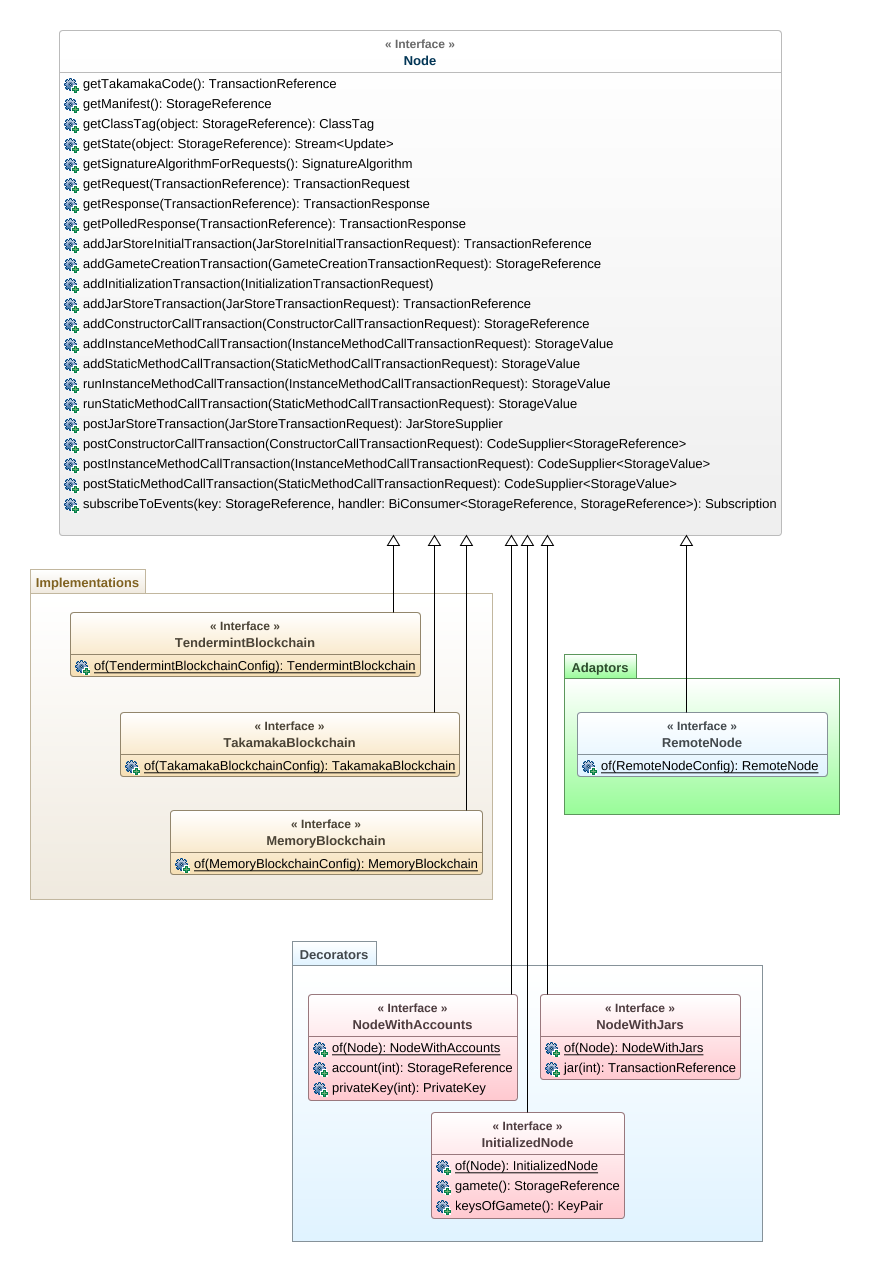
\includegraphics[width=1\textwidth,height=\textheight]{pics/nodes.png}
\caption{Figure 16. The hierarchy of Hotmoka nodes.}
\end{figure}

All Hotmoka nodes that we have deployed so far have been local objects,
living in the RAM of the same machine where we are developing our smart
contracts, or in a database of the same machine. For instance, the
\texttt{MemoryBlockchain} deployed in
\protect\hyperlink{running-the-tic-tac-toe-contract}{Running the
Tic-Tac-Toe Contract} is just an object in RAM, accessible
programmatically from the \texttt{Main} class where we create it. No
other program and no other user can access that object. The same holds
for the \texttt{TendermintBlockchain} deployed in
\protect\hyperlink{tendermint}{Running on Tendermint}, that keeps data
in a local database. In a real scenario, instead, our goal is to
\emph{publish} that object online, so that we can use it, but also other
programmers who need its service, concurrently. This must be possible
for all implementations of the \texttt{Node} interface, such as
\texttt{MemoryBlockchain} but also \texttt{TendermintBlockchain} and all
other implementations, present and future. In other words, we would like
to publish \emph{any} Hotmoka node as a service, accessible through the
internet. This will be the subject of
\protect\hyperlink{publishing-a-hotmoka-node-online}{Publishing a
Hotmoka Node Online}.

Conversely, once a Hotmoka node has been published at some internet
address, say \texttt{http://my.company.com}, it will be accessible
through some network API, through the SOAP or REST protocol, or even
through a websocket for event subscription. This complexity might make
it awkward, for a programmer, to use the published node. In that case,
we would like to create an instance of \texttt{Node} that operates as a
proxy to the network service, helping programmers integrate their
software to the service in a seamless way. This \emph{remote} node still
implements the \texttt{Node} interface. That is important since, by
programming against the \texttt{Node} interface, it will be easy for a
programmer to swap a local node with a remote node, or vice versa. This
mechanism is described in
\protect\hyperlink{building-a-hotmoka-remote-node-from-an-online-service}{Building
a Hotmoka Remote Node from an Online Service}, where the adaptor
interface \texttt{RemoteNode} in Figure 16 is presented.

\hypertarget{publishing-a-hotmoka-node-online}{%
\section{Publishing a Hotmoka Node Online
}\label{publishing-a-hotmoka-node-online}}

\textbf{{[}Run \texttt{git\ checkout\ publish\ -\/-} inside the
\texttt{hotmoka\_tutorial} repository{]}}

This section shows how we can publish a Hotmoka node online, so that it
becomes a network service that can be used, concurrently, by many users.
Namely, we will show how to publish a blockchain node based on
Tendermint, but the code is similar if you want to publish a node based
on a memory blockchain or any other Hotmoka node. Create a
\texttt{io.takamaka.publish} package inside the \texttt{blockchain}
project. Adds the following requirements (at least) to the
\texttt{module-info.java} of that project:

\begin{Shaded}
\begin{Highlighting}[]
\NormalTok{module blockchain \{}
\NormalTok{  requires io.}\FunctionTok{hotmoka}\NormalTok{.}\FunctionTok{tendermint}\NormalTok{;}
\NormalTok{  requires io.}\FunctionTok{hotmoka}\NormalTok{.}\FunctionTok{service}\NormalTok{;}
\NormalTok{  requires io.}\FunctionTok{hotmoka}\NormalTok{.}\FunctionTok{beans}\NormalTok{;}
\NormalTok{  requires io.}\FunctionTok{hotmoka}\NormalTok{.}\FunctionTok{nodes}\NormalTok{;}
\NormalTok{\}}
\end{Highlighting}
\end{Shaded}

and that its \texttt{pom.xml} reports at least the following
dependencies:

\begin{Shaded}
\begin{Highlighting}[]
\KeywordTok{<dependency>}
  \KeywordTok{<groupId>}\NormalTok{io.hotmoka}\KeywordTok{</groupId>}
  \KeywordTok{<artifactId>}\NormalTok{io-hotmoka-tendermint}\KeywordTok{</artifactId>}
  \KeywordTok{<version>}\NormalTok{1.0.0}\KeywordTok{</version>}
\KeywordTok{</dependency>}
\KeywordTok{<dependency>}
  \KeywordTok{<groupId>}\NormalTok{io.hotmoka}\KeywordTok{</groupId>}
  \KeywordTok{<artifactId>}\NormalTok{io-hotmoka-service}\KeywordTok{</artifactId>}
  \KeywordTok{<version>}\NormalTok{1.0.0}\KeywordTok{</version>}
\KeywordTok{</dependency>}
\end{Highlighting}
\end{Shaded}

Create a class \texttt{Publisher.java} inside package
\texttt{io.takamaka.publish}, whose code is the following:

\begin{Shaded}
\begin{Highlighting}[]
\KeywordTok{package}\ImportTok{ io.takamaka.publish;}

\KeywordTok{import}\ImportTok{ io.hotmoka.service.NodeService;}
\KeywordTok{import}\ImportTok{ io.hotmoka.service.NodeServiceConfig;}
\KeywordTok{import}\ImportTok{ io.hotmoka.nodes.Node;}
\KeywordTok{import}\ImportTok{ io.hotmoka.tendermint.TendermintBlockchain;}
\KeywordTok{import}\ImportTok{ io.hotmoka.tendermint.TendermintBlockchainConfig;}

\KeywordTok{public} \KeywordTok{class}\NormalTok{ Publisher \{}

  \KeywordTok{public} \DataTypeTok{static} \DataTypeTok{void} \FunctionTok{main}\NormalTok{(}\BuiltInTok{String}\NormalTok{[] args) }\KeywordTok{throws} \BuiltInTok{Exception}\NormalTok{ \{}
\NormalTok{    TendermintBlockchainConfig config = }\KeywordTok{new}\NormalTok{ TendermintBlockchainConfig.}\FunctionTok{Builder}\NormalTok{().}\FunctionTok{build}\NormalTok{();}
\NormalTok{    NodeServiceConfig serviceConfig = }\KeywordTok{new}\NormalTok{ NodeServiceConfig.}\FunctionTok{Builder}\NormalTok{().}\FunctionTok{build}\NormalTok{();}

    \KeywordTok{try}\NormalTok{ (}\BuiltInTok{Node}\NormalTok{ original = TendermintBlockchain.}\FunctionTok{of}\NormalTok{(config);}
\NormalTok{         NodeService service = NodeService.}\FunctionTok{of}\NormalTok{(serviceConfig, original)) \{}

      \BuiltInTok{System}\NormalTok{.}\FunctionTok{out}\NormalTok{.}\FunctionTok{println}\NormalTok{(}\StringTok{"}\SpecialCharTok{\textbackslash{}n}\StringTok{Press ENTER to turn off the server and exit this program"}\NormalTok{);}
      \BuiltInTok{System}\NormalTok{.}\FunctionTok{console}\NormalTok{().}\FunctionTok{readLine}\NormalTok{();}
\NormalTok{    \}}
\NormalTok{  \}}
\NormalTok{\}}
\end{Highlighting}
\end{Shaded}

We have already seen that \texttt{original} is a Hotmoka node based on
Tendermint. It is a RAM object, hence accessible from this program only.
The subsequent line makes the feat:

\begin{Shaded}
\begin{Highlighting}[]
\NormalTok{NodeService service = NodeService.}\FunctionTok{of}\NormalTok{(serviceConfig, original);}
\end{Highlighting}
\end{Shaded}

Variable \texttt{service} holds a Hotmoka \emph{service}, that is, an
actual network service that adapts the \texttt{original} node to a web
API that is published on the local host, at port 8080 (another port
number can be selected through the \texttt{serviceConfig} object, if
needed). The service is an \texttt{AutoCloseable} object: it starts when
it is created and gets shut down when its \texttt{close()} method is
invoked, which occurs, implicitly, at the end of the scope of the
try-with-resources. Hence, this service remains online until the user
presses the ENTER key and terminates the service (and the program).

Let us run this \texttt{Publisher} (the \texttt{java} invocation command
is on a single line):

\begin{myverbatim}
\begin{verbatim}
$ cd blockchain
$ mvn package
$ java --module-path $explicit:$automatic:target/blockchain-0.0.1-SNAPSHOT.jar
       -classpath $unnamed"/*"
       --module blockchain/io.takamaka.publish.Publisher
\end{verbatim}
\end{myverbatim}

The program should run and hang waiting for the ENTER key. Do not press
such key yet! Instead, try to enter the following URL into a browser
running in your machine:

\begin{myverbatim}
\begin{verbatim}
http://localhost:8080/get/signatureAlgorithmForRequests
\end{verbatim}
\end{myverbatim}

You should see the following response in your browser:

\begin{myverbatim}
\begin{verbatim}
{"algorithm":"ed25519"}
\end{verbatim}
\end{myverbatim}

What we have achieved, is to call the method
\texttt{getSignatureAlgorithmForRequests()} of \texttt{original},
accessible through the network service.

Let us try to ask for the storage address of the manifest of the node.
Again, insert the following URL in a browser on your local machine:

\begin{myverbatim}
\begin{verbatim}
http://localhost:8080/get/manifest
\end{verbatim}
\end{myverbatim}

This time, the response is negative:

\begin{Shaded}
\begin{Highlighting}[]
\FunctionTok{\{}\DataTypeTok{"message"}\FunctionTok{:}\StringTok{"no manifest set for this node"}\FunctionTok{,}
 \DataTypeTok{"exceptionClassName"}\FunctionTok{:}\StringTok{"java.util.NoSuchElementException"}\FunctionTok{\}}
\end{Highlighting}
\end{Shaded}

We have called the method \texttt{getManifest()} of \texttt{original},
through the network service. Since \texttt{original} is not initialized
yet, it has no manifest and no gamete. Its store is just empty at the
moment. Hence the negative response.

Thus, let us initialize the node before publishing it, so that it is
already initialized when published. Press ENTER to terminate the
service, then modify the \texttt{Publisher.java} class as follows:

\begin{Shaded}
\begin{Highlighting}[]
\KeywordTok{package}\ImportTok{ io.takamaka.publish;}

\KeywordTok{import static}\ImportTok{ java.math.BigInteger.ZERO;}

\KeywordTok{import}\ImportTok{ java.math.BigInteger;}
\KeywordTok{import}\ImportTok{ java.nio.file.Path;}
\KeywordTok{import}\ImportTok{ java.nio.file.Paths;}

\KeywordTok{import}\ImportTok{ io.hotmoka.service.NodeService;}
\KeywordTok{import}\ImportTok{ io.hotmoka.service.NodeServiceConfig;}
\KeywordTok{import}\ImportTok{ io.hotmoka.nodes.Node;}
\KeywordTok{import}\ImportTok{ io.hotmoka.nodes.views.InitializedNode;}
\KeywordTok{import}\ImportTok{ io.hotmoka.tendermint.TendermintBlockchain;}
\KeywordTok{import}\ImportTok{ io.hotmoka.tendermint.TendermintBlockchainConfig;}

\KeywordTok{public} \KeywordTok{class}\NormalTok{ Publisher \{}
  \KeywordTok{public} \DataTypeTok{final} \DataTypeTok{static} \BuiltInTok{BigInteger}\NormalTok{ GREEN_AMOUNT = }\BuiltInTok{BigInteger}\NormalTok{.}\FunctionTok{valueOf}\NormalTok{(}\DecValTok{100_000_000}\NormalTok{);}
  \KeywordTok{public} \DataTypeTok{final} \DataTypeTok{static} \BuiltInTok{BigInteger}\NormalTok{ RED_AMOUNT = ZERO;}

  \KeywordTok{public} \DataTypeTok{static} \DataTypeTok{void} \FunctionTok{main}\NormalTok{(}\BuiltInTok{String}\NormalTok{[] args) }\KeywordTok{throws} \BuiltInTok{Exception}\NormalTok{ \{}
\NormalTok{    Path takamakaCodePath = Paths.}\FunctionTok{get}\NormalTok{(}\StringTok{"../../hotmoka/modules/explicit/io-takamaka-code-1.0.0.jar"}\NormalTok{);}
\NormalTok{    TendermintBlockchainConfig config = }\KeywordTok{new}\NormalTok{ TendermintBlockchainConfig.}\FunctionTok{Builder}\NormalTok{().}\FunctionTok{build}\NormalTok{();}
\NormalTok{    NodeServiceConfig serviceConfig = }\KeywordTok{new}\NormalTok{ NodeServiceConfig.}\FunctionTok{Builder}\NormalTok{().}\FunctionTok{build}\NormalTok{();}

    \KeywordTok{try}\NormalTok{ (}\BuiltInTok{Node}\NormalTok{ original = TendermintBlockchain.}\FunctionTok{of}\NormalTok{(config);}
\NormalTok{         InitializedNode initialized = InitializedNode.}\FunctionTok{of}
\NormalTok{           (original, takamakaCodePath, }\StringTok{"test"}\NormalTok{, GREEN_AMOUNT, RED_AMOUNT);}
\NormalTok{         NodeService service = NodeService.}\FunctionTok{of}\NormalTok{(serviceConfig, original)) \{}

      \BuiltInTok{System}\NormalTok{.}\FunctionTok{out}\NormalTok{.}\FunctionTok{println}\NormalTok{(}\StringTok{"}\SpecialCharTok{\textbackslash{}n}\StringTok{Press ENTER to turn off the server and exit this program"}\NormalTok{);}
      \BuiltInTok{System}\NormalTok{.}\FunctionTok{console}\NormalTok{().}\FunctionTok{readLine}\NormalTok{();}
\NormalTok{    \}}
\NormalTok{  \}}
\NormalTok{\}}
\end{Highlighting}
\end{Shaded}

\begin{quote}
Note that we have published \texttt{original}:

\begin{Shaded}
\begin{Highlighting}[]
\NormalTok{NodeService service = NodeService.}\FunctionTok{of}\NormalTok{(serviceConfig, original);}
\end{Highlighting}
\end{Shaded}

We could have published \texttt{initialized} instead:

\begin{Shaded}
\begin{Highlighting}[]
\NormalTok{NodeService service = NodeService.}\FunctionTok{of}\NormalTok{(serviceConfig, initialized);}
\end{Highlighting}
\end{Shaded}

The result would be the same, since both are views of the same node
object.
\end{quote}

If you re-package the \texttt{blockchain} project, re-run it with
\texttt{java} and re-enter the last URL in a browser on your local
machine, the response will be positive this time:

\begin{Shaded}
\begin{Highlighting}[]
\FunctionTok{\{}
  \DataTypeTok{"transaction"}\FunctionTok{:}
  \FunctionTok{\{}
    \DataTypeTok{"type"}\FunctionTok{:}\StringTok{"local"}\FunctionTok{,}
    \DataTypeTok{"hash"}\FunctionTok{:}\StringTok{"f9ac8849f7ee484d73fd84470652582cf93da97c379fee9ccc66bd5e2ffc9867"}
  \FunctionTok{\},}
  \DataTypeTok{"progressive"}\FunctionTok{:}\StringTok{"0"}
\FunctionTok{\}}
\end{Highlighting}
\end{Shaded}

This means that the manifest is held, in the store of \texttt{original},
at the storage reference
\texttt{f9ac8849f7ee484d73fd84470652582cf93da97c379fee9ccc66bd5e2ffc9867\#0}.

The natural question is now: should one publish the node initialized or
still uninitialized? Both possibilities are sensible, but each matches a
different scenario. In a real blockchain, composed by many
interconnected published nodes, only one node will be published
initialized, while the others will be published uninitialized and will
synchronize by consensus, hence ending up being initialized as well,
after a few seconds.

\begin{quote}
A Hotmoka node, once published, can be accessed by many users,
\emph{concurrently}. This is not a problem, since Hotmoka nodes are
thread-safe and can be used in parallel by many users. Of course, this
does not mean that there are no race conditions at the application
level. As a simple example, if two users operate with the same paying
externally owned account, their wallets might suffer from race
conditions on the nonce of the account and they might see requests
rejected because of an incorrect nonce. The situation is the same here
as in Ethereum, for instance. In practice, each externally owned account
should be controlled by a single user.
\end{quote}

\hypertarget{publishing-a-hotmoka-node-on-amazon-ec2}{%
\subsection{Publishing a Hotmoka Node on Amazon EC2
}\label{publishing-a-hotmoka-node-on-amazon-ec2}}

We have published the node on our machine (the local host). This might
not be the best place where a Hotmoka node should be published, since
our machine might not allow external connections from the internet and
since we might want to turn it off after we stop working with it. In
reality, a node should be published on a machine that can receive
external connections and that is always on, at least for a long period.
There are many solutions for that. Here, we describe the simple
technique of using a rented machine from Amazon AWS EC2 computing cloud
\protect\hyperlink{EC2}{{[}EC2{]}}. This service offers a micro machine
for free, while more powerful machines require one to pay for their use.
Since the micro machine is enough for our purposes, EC2 is a good
candidate for experimentation.

First of all, we want to publish an empty node. This means that the
first thing you should do is to come back to the first version of
\texttt{Publisher.java} (as at the beginning of Section
\protect\hyperlink{publishing-a-hotmoka-node-online}{Publishing a
Hotmoka Node Online}) and re-package the \texttt{blockchain} project:

\begin{myverbatim}
\begin{verbatim}
$ cd blockchain
$ mvn package
\end{verbatim}
\end{myverbatim}

Perform then the following steps in order to publish a node online with
Amazon EC2:

\begin{enumerate}
\def\labelenumi{\arabic{enumi}.}
\tightlist
\item
  turn on an Amazon EC2 machine from the AWS console
\item
  edit the inbound rules of the security group of the machine so that
  its port 8080 is open for every incoming TCP connection
\item
  install the Java Runtime Environment in the machine, at least version
  11
\item
  install Tendermint in the machine, if you plan to publish a Tendermint
  Hotmoka node
\item
  transfer the \texttt{modules} directory of the \texttt{hotmoka}
  project from your local machine to the EC2 machine; do not forget to
  include, in the \texttt{modules/explicit} directory, also the jar of
  our \texttt{blockchain} project, since it contains our code that
  publishes the node. You can transfer the directory with a command such
  as the following one, where you have to specify your identity pem file
  and use the name of your EC2 machine. We have used ours as an example:
\end{enumerate}

\begin{myverbatim}
\begin{verbatim}
$ scp -r -i your.pem modules/* ubuntu@ec2-99-80-8-84.eu-west-1.compute.amazonaws.com:
\end{verbatim}
\end{myverbatim}

\begin{enumerate}
\def\labelenumi{\arabic{enumi}.}
\setcounter{enumi}{5}
\tightlist
\item
  connect to the EC2 machine:
\end{enumerate}

\begin{myverbatim}
\begin{verbatim}
$ ssh -i your.pem ubuntu@ec2-99-80-8-84.eu-west-1.compute.amazonaws.com
\end{verbatim}
\end{myverbatim}

\begin{enumerate}
\def\labelenumi{\arabic{enumi}.}
\setcounter{enumi}{6}
\tightlist
\item
  start the server there and leave it running in the background (the
  following commands must be done in the EC2 machine):
\end{enumerate}

\begin{myverbatim}
\begin{verbatim}
$ screen
$ cwd=$(pwd)
$ explicit=$cwd"/modules/explicit"
$ automatic=$cwd"/modules/automatic"
$ unnamed=$cwd"/modules/unnamed"
$ java --module-path $explicit:$automatic:target/blockchain-0.0.1-SNAPSHOT.jar
       -classpath $unnamed"/*"
       --module blockchain/io.takamaka.publish.Publisher
[wait until the Java program asks to press ENTER]
$ CTRL-a d
$ exit
\end{verbatim}
\end{myverbatim}

The \texttt{screen} command allows us to exit the remote shell and leave
the \texttt{java} process running in the background.

You can verify that the EC2 server is accessible from outside if you
direct your local browser to it and connect to:

\begin{myverbatim}
\begin{verbatim}
http://ec2-99-80-8-84.eu-west-1.compute.amazonaws.com:8080/get/manifest
\end{verbatim}
\end{myverbatim}

The response should be something like:

\begin{Shaded}
\begin{Highlighting}[]
\FunctionTok{\{}\DataTypeTok{"message"}\FunctionTok{:}\StringTok{"no manifest set for this node"}\FunctionTok{,}
 \DataTypeTok{"exceptionClassName"}\FunctionTok{:}\StringTok{"java.util.NoSuchElementException"}\FunctionTok{\}}
\end{Highlighting}
\end{Shaded}

since we have published an empty node.

\hypertarget{building-a-hotmoka-remote-node-from-an-online-service}{%
\section{Building a Hotmoka Remote Node from an Online Service
}\label{building-a-hotmoka-remote-node-from-an-online-service}}

\textbf{{[}Run \texttt{git\ checkout\ remote\ -\/-} inside the
\texttt{hotmoka\_tutorial} repository{]}}

We have seen how a service can be published and its methods can be
called through a browser. This has been easy for methods such as
\texttt{getManifest()} and \texttt{getSignatureAlgorithmForRequest()} of
the interface \texttt{Node}. However, it becomes harder if we want to
call methods of \texttt{Node} that need parameters, such as
\texttt{getState()} or the many \texttt{add/post/run} methods for
scheduling transactions on the node. Parameters should be passed as JSON
payload of the http connection, in a format that is hard to remember,
easy to get wrong and possibly changing in the future. Moreover, the
JSON responses must be parsed back. In principle, this can be done by
hand or through software that builds the requests for the server and
interprets its responses. Nevertheless, it is not the suggested way to
proceed. Imagine to do all that for each transaction request in the test
class of \protect\hyperlink{running-the-tic-tac-toe-contract}{Running
the Tic-Tac-Toe Contract}!

A typical solution to this problem is to provide a software SDK, that
is, a library that takes care of serializing the requests into JSON and
deserializing the responses from JSON. Roughly speaking, this is the
approach taken in Hotmoka. More precisely, as this section will show, we
can forget about the details of the JSON serialization and
deserialization of requests and responses and only program against the
\texttt{Node} interface, by using an adaptor of a published Hotmoka
service into a \texttt{Node}. This adaptor is called a \emph{remote}
Hotmoka node.

In the experiment that we are going to perform, we will run, on a remote
node, the test class of the tic-tac-toe game from section
\protect\hyperlink{running-the-tic-tac-toe-contract}{Running the
Tic-Tac-Toe Contract}. Consider its class
\texttt{io.takamaka.tictactoe.Main.java}. Currently, it creates a local
node to run the transactions:

\begin{Shaded}
\begin{Highlighting}[]
\NormalTok{...}
\KeywordTok{import}\ImportTok{ io.hotmoka.memory.MemoryBlockchain;}
\KeywordTok{import}\ImportTok{ io.hotmoka.memory.MemoryBlockchainConfig;}
\NormalTok{...}
\KeywordTok{public} \KeywordTok{class}\NormalTok{ Main \{}
\NormalTok{  ...}
  \KeywordTok{public} \DataTypeTok{static} \DataTypeTok{void} \FunctionTok{main}\NormalTok{(}\BuiltInTok{String}\NormalTok{[] args) }\KeywordTok{throws} \BuiltInTok{Exception}\NormalTok{ \{}
\NormalTok{    MemoryBlockchainConfig config = }\KeywordTok{new}\NormalTok{ MemoryBlockchainConfig.}\FunctionTok{Builder}\NormalTok{().}\FunctionTok{build}\NormalTok{();}
\NormalTok{    ...}
    \KeywordTok{try}\NormalTok{ (}\BuiltInTok{Node}\NormalTok{ node = MemoryBlockchain.}\FunctionTok{of}\NormalTok{(config)) \{ }\KeywordTok{... }\NormalTok{\}}
\NormalTok{  \}}
\NormalTok{\}}
\end{Highlighting}
\end{Shaded}

Swapping to a remote node is very easy:

\begin{Shaded}
\begin{Highlighting}[]
\NormalTok{...}
\KeywordTok{import}\ImportTok{ io.hotmoka.remote.RemoteNode;}
\KeywordTok{import}\ImportTok{ io.hotmoka.remote.RemoteNodeConfig;}
\NormalTok{...}
\KeywordTok{public} \KeywordTok{class}\NormalTok{ Main \{}
\NormalTok{  ...}
  \KeywordTok{public} \DataTypeTok{static} \DataTypeTok{void} \FunctionTok{main}\NormalTok{(}\BuiltInTok{String}\NormalTok{[] args) }\KeywordTok{throws} \BuiltInTok{Exception}\NormalTok{ \{}
\NormalTok{    RemoteNodeConfig config = }\KeywordTok{new}\NormalTok{ RemoteNodeConfig.}\FunctionTok{Builder}\NormalTok{()}
\NormalTok{      .}\FunctionTok{setURL}\NormalTok{(}\StringTok{"ec2-99-80-8-84.eu-west-1.compute.amazonaws.com:8080"}\NormalTok{)}
\NormalTok{      .}\FunctionTok{build}\NormalTok{();}
\NormalTok{    ...}
    \KeywordTok{try}\NormalTok{ (}\BuiltInTok{Node}\NormalTok{ node = RemoteNode.}\FunctionTok{of}\NormalTok{(config)) \{ }\KeywordTok{... }\NormalTok{\}}
\NormalTok{  \}}
\NormalTok{\}}
\end{Highlighting}
\end{Shaded}

\begin{quote}
If you have not published a node on a remote machine, as shown in the
previous section, publish it on the local host and change the URL:

\begin{Shaded}
\begin{Highlighting}[]
\NormalTok{ RemoteNodeConfig config = }\KeywordTok{new}\NormalTok{ RemoteNodeConfig.}\FunctionTok{Builder}\NormalTok{()}
\NormalTok{   .}\FunctionTok{setURL}\NormalTok{(}\StringTok{"localhost:8080"}\NormalTok{)}
\NormalTok{   .}\FunctionTok{build}\NormalTok{();}
\end{Highlighting}
\end{Shaded}
\end{quote}

Only four lines of code needed to be touched! The rest of the test class
remains unchanged, since it works against the \texttt{Node} interface
and remote nodes implement the \texttt{Node} interface.

You can now package the \texttt{blockchain} project and run the test
class (the \texttt{java} invocation command is on a single line):

\begin{myverbatim}
\begin{verbatim}
$ cd blockchain
$ mvn package
$ java --module-path $explicit:$automatic:target/blockchain-0.0.1-SNAPSHOT.jar
       -classpath $unnamed"/*"
       --module blockchain/io.takamaka.tictactoe.Main
\end{verbatim}
\end{myverbatim}

The result should be the same as in
\protect\hyperlink{running-the-tic-tac-toe-contract}{Running the
Tic-Tac-Toe Contract}, with the difference that the transactions have
been executed on the remote machine now, while our local machine has
just sent the requests and received the responses.

By default, a remote node connects to a service by using the HTTP
protocol, but handles event notification by using web sockets. This is
automatic and you do not need to understand the details of this
connection. It is possible to use web sockets for all communications,
also those of the many \texttt{get/add/post/run} methods of the
\texttt{Node} interface. For that, you can set a flag in the
configuration of the remote node, as follows:

\begin{Shaded}
\begin{Highlighting}[]
\NormalTok{RemoteNodeConfig config = }\KeywordTok{new}\NormalTok{ RemoteNodeConfig.}\FunctionTok{Builder}\NormalTok{()}
\NormalTok{  .}\FunctionTok{setURL}\NormalTok{(}\StringTok{"ec2-99-80-8-84.eu-west-1.compute.amazonaws.com:8080"}\NormalTok{)}
\NormalTok{  .}\FunctionTok{setWebSockets}\NormalTok{(}\KeywordTok{true}\NormalTok{)}
\NormalTok{  .}\FunctionTok{build}\NormalTok{();}
\end{Highlighting}
\end{Shaded}

Nevertheless, there is currently no actual benefit in using web sockets
for all communications. Thus, we suggest you to stick to the default
configuration, that uses web sockest only for event notification to the
subscribed event handlers.

\hypertarget{creating-sentry-nodes}{%
\subsection{Creating Sentry Nodes }\label{creating-sentry-nodes}}

We have seen that a \texttt{Node} can be published as a Hotmoka service:
on a machine \texttt{my.validator.com} we can execute:

\begin{Shaded}
\begin{Highlighting}[]
\NormalTok{TendermintBlockchainConfig config = }\KeywordTok{new}\NormalTok{ TendermintBlockchainConfig.}\FunctionTok{Builder}\NormalTok{().}\FunctionTok{build}\NormalTok{();}
\NormalTok{NodeServiceConfig serviceConfig = }\KeywordTok{new}\NormalTok{ NodeServiceConfig.}\FunctionTok{Builder}\NormalTok{().}\FunctionTok{build}\NormalTok{();}

\KeywordTok{try}\NormalTok{ (}\BuiltInTok{Node}\NormalTok{ original = TendermintBlockchain.}\FunctionTok{of}\NormalTok{(config);}
\NormalTok{     NodeService service = NodeService.}\FunctionTok{of}\NormalTok{(serviceConfig, original)) \{}
\NormalTok{  ...}
\NormalTok{\}}
\end{Highlighting}
\end{Shaded}

The service will be available on the internet as

\begin{myverbatim}
\begin{verbatim}
http://my.validator.com:8080
\end{verbatim}
\end{myverbatim}

Moreover, on another machine \texttt{my.sentry.com} that Hotmoka service
can be adapted into a (\emph{remote}) \texttt{Node} that, itself, can be
published on that machine:

\begin{Shaded}
\begin{Highlighting}[]
\NormalTok{NodeServiceConfig serviceConfig = }\KeywordTok{new}\NormalTok{ NodeServiceConfig.}\FunctionTok{Builder}\NormalTok{().}\FunctionTok{build}\NormalTok{();}
\NormalTok{RemoteNodeConfig config = }\KeywordTok{new}\NormalTok{ RemoteNodeConfig.}\FunctionTok{Builder}\NormalTok{()}
\NormalTok{  .}\FunctionTok{setURL}\NormalTok{(}\StringTok{"my.validator.com:8080"}\NormalTok{)}
\NormalTok{  .}\FunctionTok{build}\NormalTok{();}

\KeywordTok{try}\NormalTok{ (}\BuiltInTok{Node}\NormalTok{ validator = RemoteNode.}\FunctionTok{of}\NormalTok{(config);}
\NormalTok{     NodeService service = NodeService.}\FunctionTok{of}\NormalTok{(serviceConfig, validator)) \{}
\NormalTok{  ...}
\NormalTok{\}}
\end{Highlighting}
\end{Shaded}

The service will be available at

\begin{myverbatim}
\begin{verbatim}
http://my.sentry.com:8080
\end{verbatim}
\end{myverbatim}

We can continue this process as much as we want, but let us stop at this
point. Programmers can connect to the service published at
\texttt{http://my.sentry.com:8080} and send requests to it. That service
is just a bridge that forwards everything to the service at
\texttt{http://my.validator.com:8080}. It might not be immediately clear
why this intermediate step could be useful or desirable. The motivation
is that we could keep the (precious) validator machine under a firewall
that allows connections with \texttt{my.sentry.com} only. As a
consequence, in case of DOS attacks, the sentry node will receive the
attack and possibly crash, while the validator continues to operate as
usual. Since many sentries can be connected to a single validator, the
latter remains accessible through the other sentries. This is an
effective way to mitigate the problem of DOS attacks to validator nodes.

The idea of sentry nodes against DOS attacks is not new and is used, for
instance, in Cosmos networks \protect\hyperlink{Sentry}{{[}Sentry{]}}.
However, note how easy it is, with Hotmoka, to build such a network
architecture by using network services and remote nodes.

\hypertarget{signatures-and-quantum-resistance}{%
\section{Signatures and Quantum-Resistance
}\label{signatures-and-quantum-resistance}}

\textbf{{[}Run \texttt{git\ checkout\ signatures\ -\/-} inside the
\texttt{hotmoka\_tutorial} repository{]}}

Hotmoka is agnostic wrt. the algorithm used for signing requests. This
means that it is possible to deploy Hotmoka nodes that sign requests
with distinct signature algorithms. Of course, if nodes must re-execute
the same transactions, such as in the case of a blockchain, then all
nodes of the blockchain must use the same algorithm, or otherwise they
will not be able to reach consensus. Yet, any algorithm can be chosen
for the blockchain. In principle, it is even possible to use an
algorithm that does not sign the transactions, if the identity of the
callers of the transactions needn't be verified. However, this might be
sensible in local networks only.

The default signature algorithm used by a node is specified at
construction time, as a configuration parameter. For instance, the code

\begin{Shaded}
\begin{Highlighting}[]
\NormalTok{TendermintBlockchainConfig config = }\KeywordTok{new}\NormalTok{ TendermintBlockchainConfig.}\FunctionTok{Builder}\NormalTok{()}
\NormalTok{                                      .}\FunctionTok{signRequestsWith}\NormalTok{(}\StringTok{"ed25519"}\NormalTok{)}
\NormalTok{                                      .}\FunctionTok{build}\NormalTok{();}

\KeywordTok{try}\NormalTok{ (}\BuiltInTok{Node}\NormalTok{ node = TendermintBlockchain.}\FunctionTok{of}\NormalTok{(config)) \{}
\NormalTok{  ...}
\NormalTok{\}}
\end{Highlighting}
\end{Shaded}

starts a Tendermint-based blockchain node that uses the ed25519
signature algorithm as default signature algorithm for the requests.
Requests sent to that node can be signed as follows:

\begin{Shaded}
\begin{Highlighting}[]
\CommentTok{// recover the algorihm used by the node}
\NormalTok{SignatureAlgorithm<SignedTransactionRequest> signature}
\NormalTok{  = node.}\FunctionTok{getSignatureAlgorithmForRequests}\NormalTok{();}

\CommentTok{// create a key pair for that algorithm}
\BuiltInTok{KeyPair}\NormalTok{ keys = signature.}\FunctionTok{getKeyPair}\NormalTok{();}

\CommentTok{// create a signer object with the private key of the key pair}
\BuiltInTok{Signer}\NormalTok{ signer = }\BuiltInTok{Signer}\NormalTok{.}\FunctionTok{with}\NormalTok{(signature, keys.}\FunctionTok{getPrivate}\NormalTok{());}

\CommentTok{// create an account having public key keys.getPublic()}
\NormalTok{....}

\CommentTok{// create a transaction request on behalf of the account}
\NormalTok{ConstructorCallTransactionRequest request}
\NormalTok{  = }\KeywordTok{new} \FunctionTok{ConstructorCallTransactionRequest}\NormalTok{(signer, account, ...);}

\CommentTok{// send the request to the node}
\NormalTok{node.}\FunctionTok{addConstructorCallTransaction}\NormalTok{(request);}
\end{Highlighting}
\end{Shaded}

In the example above, we have explicitly specified to use ed25519 as
default signature algorithm. That is what is chosen if nothing is
specified at configuration-time. Consequently, there is no need to
specify that algorithm in the configuration object and that is why we
never did it in the previous chapters. It is possible to configure nodes
with other default signature algorithms. For instance,

\begin{Shaded}
\begin{Highlighting}[]
\NormalTok{TendermintBlockchainConfig config = }\KeywordTok{new}\NormalTok{ TendermintBlockchainConfig.}\FunctionTok{Builder}\NormalTok{()}
\NormalTok{                                      .}\FunctionTok{signRequestsWith}\NormalTok{(}\StringTok{"sha256dsa"}\NormalTok{)}
\NormalTok{                                      .}\FunctionTok{build}\NormalTok{();}
\end{Highlighting}
\end{Shaded}

configures a node that uses the sha256dsa as default signature
algorithm, while

\begin{Shaded}
\begin{Highlighting}[]
\NormalTok{TendermintBlockchainConfig config = }\KeywordTok{new}\NormalTok{ TendermintBlockchainConfig.}\FunctionTok{Builder}\NormalTok{()}
\NormalTok{                                      .}\FunctionTok{signRequestsWith}\NormalTok{(}\StringTok{"empty"}\NormalTok{)}
\NormalTok{                                      .}\FunctionTok{build}\NormalTok{();}
\end{Highlighting}
\end{Shaded}

configures a node that uses the empty signature as default signature
algorithm; it is an algorithm that accepts all signatures, in practice
disabling any signature checking.

It is possible to specify a quantum-resistant signature algorithm as
default, that is, one that belongs to a family of algorithms that are
expected to be immune from attacks performed through a quantistic
computer. For instance,

\begin{Shaded}
\begin{Highlighting}[]
\NormalTok{TendermintBlockchainConfig config = }\KeywordTok{new}\NormalTok{ TendermintBlockchainConfig.}\FunctionTok{Builder}\NormalTok{()}
\NormalTok{                                      .}\FunctionTok{signRequestsWith}\NormalTok{(}\StringTok{"qtesla1"}\NormalTok{)}
\NormalTok{                                      .}\FunctionTok{build}\NormalTok{();}
\end{Highlighting}
\end{Shaded}

configures a node that uses the quantum-resistant qtesla-p-I algorithm
as default signature algorihtm, while

\begin{Shaded}
\begin{Highlighting}[]
\NormalTok{TendermintBlockchainConfig config = }\KeywordTok{new}\NormalTok{ TendermintBlockchainConfig.}\FunctionTok{Builder}\NormalTok{()}
\NormalTok{                                      .}\FunctionTok{signRequestsWith}\NormalTok{(}\StringTok{"qtesla3"}\NormalTok{)}
\NormalTok{                                      .}\FunctionTok{build}\NormalTok{();}
\end{Highlighting}
\end{Shaded}

configures a node that uses the quantum-resistant qtesla-p-III algorithm
as default signature algorihtm, that is expected to be more resistent
than qtesla-p-III but has larger signatures than qtesla-p-I.

Quantum-resistance is an important aspect of future-generation
blockchains. However, at the time of this writing, a quantum attack is
mainly a theoretical possibility, while the large size of
quantum-resistant keys and signatures is already a reality and a node
using a qtesla signature algorithm \emph{as default} might exhaust the
disk space of your computer very quickly. In practice, it is better to
use a quantum-resistant algorithm only for a subset of the transactions,
whose quantum-resistance is deemed important. Instead, one should use a
lighter algorithm (such as the default ed25519) for all other
transactions. This is possible because Hotmoka nodes allow one to mix
transactions signed with distinct algorithms. For instance, one could
use ed25519 as default algorithm, for all transactions signed by
instances of \texttt{ExternallyOwnedAccount}s, with the exception of
those transactions that are signed by instances of
\texttt{AccountQTESLA1}, such as \texttt{ExternallyOwnedAccountQTESLA1},
or of \texttt{AccountQTESLA3}, such as
\texttt{ExternallOwnedAccountQTESLA3}, or of \texttt{AccountSHA256DSA},
such as \texttt{ExternallOwnedAccountSHA256DSA} (see Figure 7). Namely,
if the caller of a transaction is an \texttt{AccountQTESLA1}, then the
request of the transaction will always be signed with the qtesla-p-I
algorithm. If the caller of a transaction is an \texttt{AccountQTESLA3},
then the request of the transaction will always be signed with the
qtesla-p-III algorithm. If the caller of a transaction is an
\texttt{AccountSHA256DSA}, then the request of the transaction will
always be signed with the sha256dsa algorithm. If the caller of a
transaction is an \texttt{AccountED25519}, then the request of the
transaction will always be signed with the ed25519 algorithm. In
practice, this allows specific transactions to override the default
signature algorithm for the node.

For instance, let us write some code that starts a node that uses the
default ed25519 signature algorithm, then creates an
\texttt{ExternallyOwnedAccountQTESLA1} account (passing a qtesla public
key to its constructor), uses that account to sign a transaction with
the qtesla-p-I signature algorithm and finally runs that transaction on
the node. For that, create a package \texttt{io.takamaka.signatures}
inside the \texttt{blockchain} project and copy the following
\texttt{Main.java} inside that package:

\begin{Shaded}
\begin{Highlighting}[]
\KeywordTok{package}\ImportTok{ io.takamaka.signatures;}

\KeywordTok{import static}\ImportTok{ java.math.BigInteger.TWO;}
\KeywordTok{import static}\ImportTok{ java.math.BigInteger.ONE;}
\KeywordTok{import static}\ImportTok{ java.math.BigInteger.ZERO;}

\KeywordTok{import}\ImportTok{ java.math.BigInteger;}
\KeywordTok{import}\ImportTok{ java.nio.file.Path;}
\KeywordTok{import}\ImportTok{ java.nio.file.Paths;}
\KeywordTok{import}\ImportTok{ java.security.KeyPair;}
\KeywordTok{import}\ImportTok{ java.util.Base64;}

\KeywordTok{import}\ImportTok{ io.hotmoka.beans.requests.ConstructorCallTransactionRequest;}
\KeywordTok{import}\ImportTok{ io.hotmoka.beans.requests.SignedTransactionRequest;}
\KeywordTok{import}\ImportTok{ io.hotmoka.beans.requests.SignedTransactionRequest.Signer;}
\KeywordTok{import}\ImportTok{ io.hotmoka.beans.requests.StaticMethodCallTransactionRequest;}
\KeywordTok{import}\ImportTok{ io.hotmoka.beans.signatures.ConstructorSignature;}
\KeywordTok{import}\ImportTok{ io.hotmoka.beans.signatures.NonVoidMethodSignature;}
\KeywordTok{import}\ImportTok{ io.hotmoka.beans.types.BasicTypes;}
\KeywordTok{import}\ImportTok{ io.hotmoka.beans.types.ClassType;}
\KeywordTok{import}\ImportTok{ io.hotmoka.beans.values.BigIntegerValue;}
\KeywordTok{import}\ImportTok{ io.hotmoka.beans.values.IntValue;}
\KeywordTok{import}\ImportTok{ io.hotmoka.beans.values.LongValue;}
\KeywordTok{import}\ImportTok{ io.hotmoka.beans.values.StorageReference;}
\KeywordTok{import}\ImportTok{ io.hotmoka.beans.values.StringValue;}
\KeywordTok{import}\ImportTok{ io.hotmoka.crypto.SignatureAlgorithm;}
\KeywordTok{import}\ImportTok{ io.hotmoka.nodes.Node;}
\KeywordTok{import}\ImportTok{ io.hotmoka.nodes.views.InitializedNode;}
\KeywordTok{import}\ImportTok{ io.hotmoka.tendermint.TendermintBlockchain;}
\KeywordTok{import}\ImportTok{ io.hotmoka.tendermint.TendermintBlockchainConfig;}

\KeywordTok{public} \KeywordTok{class}\NormalTok{ Main \{}
  \KeywordTok{public} \DataTypeTok{final} \DataTypeTok{static} \BuiltInTok{BigInteger}\NormalTok{ GREEN_AMOUNT = }\BuiltInTok{BigInteger}\NormalTok{.}\FunctionTok{valueOf}\NormalTok{(}\DecValTok{100_000_000}\NormalTok{);}
  \KeywordTok{public} \DataTypeTok{final} \DataTypeTok{static} \BuiltInTok{BigInteger}\NormalTok{ RED_AMOUNT = ZERO;}

  \KeywordTok{public} \DataTypeTok{static} \DataTypeTok{void} \FunctionTok{main}\NormalTok{(}\BuiltInTok{String}\NormalTok{[] args) }\KeywordTok{throws} \BuiltInTok{Exception}\NormalTok{ \{}
    \CommentTok{// the blockhain uses ed25519 as default}
\NormalTok{    TendermintBlockchainConfig config = }\KeywordTok{new}\NormalTok{ TendermintBlockchainConfig.}\FunctionTok{Builder}\NormalTok{().}\FunctionTok{build}\NormalTok{();}

    \CommentTok{// the path of the packaged runtime Takamaka classes}
\NormalTok{    Path takamakaCodePath = Paths.}\FunctionTok{get}
\NormalTok{      (}\StringTok{"../../hotmoka/modules/explicit/io-takamaka-code-1.0.0.jar"}\NormalTok{);}

    \KeywordTok{try}\NormalTok{ (}\BuiltInTok{Node}\NormalTok{ node = TendermintBlockchain.}\FunctionTok{of}\NormalTok{(config)) \{}
      \CommentTok{// store io-takamaka-code-1.0.0.jar and create manifest and gamete}
\NormalTok{      InitializedNode initialized = InitializedNode.}\FunctionTok{of}
\NormalTok{        (node, takamakaCodePath, }\StringTok{"test"}\NormalTok{, GREEN_AMOUNT, RED_AMOUNT);}

      \CommentTok{// get the algorithm for qtesla-p-I signatures}
\NormalTok{      SignatureAlgorithm<SignedTransactionRequest> qtesla = SignatureAlgorithm.}\FunctionTok{qtesla1}
\NormalTok{        (SignedTransactionRequest::toByteArrayWithoutSignature);}

      \CommentTok{// create a qtesla keypair}
      \BuiltInTok{KeyPair}\NormalTok{ qteslaKeyPair = qtesla.}\FunctionTok{getKeyPair}\NormalTok{();}

      \CommentTok{// transform the public qtesla key into a Base64-encoded string}
\NormalTok{      StringValue qteslaPublicKey = }\KeywordTok{new}\NormalTok{ StringValue}
\NormalTok{        (Base64.}\FunctionTok{getEncoder}\NormalTok{().}\FunctionTok{encodeToString}\NormalTok{(qteslaKeyPair.}\FunctionTok{getPublic}\NormalTok{().}\FunctionTok{getEncoded}\NormalTok{()));}

      \CommentTok{// create an account with 100,000 units of coin:}
      \CommentTok{// it will use the qtesla-p-I algorithm for signing transactions,}
      \CommentTok{// regardless of the default used for the blockchain}
\NormalTok{      StorageReference qteslaAccount = node.}\FunctionTok{addConstructorCallTransaction}
\NormalTok{       (}\KeywordTok{new}\NormalTok{ ConstructorCallTransactionRequest}
        \CommentTok{// signed with the default algorithm}
\NormalTok{        (}\BuiltInTok{Signer}\NormalTok{.}\FunctionTok{with}\NormalTok{(node.}\FunctionTok{getSignatureAlgorithmForRequests}\NormalTok{(),}
\NormalTok{            initialized.}\FunctionTok{keysOfGamete}\NormalTok{()),}
\NormalTok{         initialized.}\FunctionTok{gamete}\NormalTok{(), }\CommentTok{// the gamete is the caller}
\NormalTok{         TWO, }\CommentTok{// nonce}
         \StringTok{"test"}\NormalTok{, }\CommentTok{// chain id}
         \BuiltInTok{BigInteger}\NormalTok{.}\FunctionTok{valueOf}\NormalTok{(}\DecValTok{50_000}\NormalTok{), }\CommentTok{// gas amount}
\NormalTok{         ONE, }\CommentTok{// gas cost}
\NormalTok{         initialized.}\FunctionTok{getTakamakaCode}\NormalTok{(), }\CommentTok{// classpath}
         \CommentTok{// call the constructor of}
         \CommentTok{// ExternallyOwnedAccountQTESLA1(int amount, String publicKey)}
         \KeywordTok{new}\NormalTok{ ConstructorSignature}
\NormalTok{           (}\StringTok{"io.takamaka.code.lang.ExternallyOwnedAccountQTESLA1"}\NormalTok{,}
\NormalTok{            BasicTypes.}\FunctionTok{INT}\NormalTok{, ClassType.}\FunctionTok{STRING}\NormalTok{),}
         \KeywordTok{new} \FunctionTok{IntValue}\NormalTok{(}\DecValTok{100_000}\NormalTok{), }\CommentTok{// the amount}
\NormalTok{         qteslaPublicKey)); }\CommentTok{// the qtesla public key of the account}

      \CommentTok{// use the qtesla account to call the following static method}
      \CommentTok{// of the Takamaka library:}
      \CommentTok{// BigInteger io.takamaka.code.lang.Coin.panarea(long)}
\NormalTok{      NonVoidMethodSignature callee = }\KeywordTok{new}\NormalTok{ NonVoidMethodSignature}
\NormalTok{        (}\StringTok{"io.takamaka.code.lang.Coin"}\NormalTok{, }\StringTok{"panarea"}\NormalTok{,}
\NormalTok{         ClassType.}\FunctionTok{BIG_INTEGER}\NormalTok{, BasicTypes.}\FunctionTok{LONG}\NormalTok{);}

      \CommentTok{// the next transaction will be signed with the qtesla signature since this is}
      \CommentTok{// what the qtesla account uses, regardless of the default algorithm of the node}
\NormalTok{      BigIntegerValue result = (BigIntegerValue) node.}\FunctionTok{addStaticMethodCallTransaction}
\NormalTok{       (}\KeywordTok{new}\NormalTok{ StaticMethodCallTransactionRequest}
\NormalTok{        (}\BuiltInTok{Signer}\NormalTok{.}\FunctionTok{with}\NormalTok{(qtesla, qteslaKeyPair), }\CommentTok{// signed with the qtesla algorithm}
\NormalTok{         qteslaAccount, }\CommentTok{// the caller is the qtesla account}
\NormalTok{         ZERO, }\CommentTok{// the nonce of the gtesla account}
         \StringTok{"test"}\NormalTok{, }\CommentTok{// the chain id}
         \BuiltInTok{BigInteger}\NormalTok{.}\FunctionTok{valueOf}\NormalTok{(}\DecValTok{20_000}\NormalTok{), }\CommentTok{// gas amount}
\NormalTok{         ONE, }\CommentTok{// gas cost}
\NormalTok{         initialized.}\FunctionTok{getTakamakaCode}\NormalTok{(), }\CommentTok{// classpath}
\NormalTok{         callee, }\CommentTok{// the static method to class}
         \KeywordTok{new} \FunctionTok{LongValue}\NormalTok{(}\DecValTok{1973}\NormalTok{))); }\CommentTok{// actual argument}

      \BuiltInTok{System}\NormalTok{.}\FunctionTok{out}\NormalTok{.}\FunctionTok{println}\NormalTok{(}\StringTok{"result = "}\NormalTok{ + result);}
\NormalTok{    \}}
\NormalTok{  \}}
\NormalTok{\}}
\end{Highlighting}
\end{Shaded}

You can now package the \texttt{blockchain} project and run the class
(the \texttt{java} invocation command is on a single line):

\begin{myverbatim}
\begin{verbatim}
$ cd blockchain
$ mvn package
$ java --module-path $explicit:$automatic:target/blockchain-0.0.1-SNAPSHOT.jar
       -classpath $unnamed"/*"
       --module blockchain/io.takamaka.signatures.Main
\end{verbatim}
\end{myverbatim}

The transactions will be executed, with distinct signature algorithms,
and the return value of the static method of class \texttt{Coin} will be
printed on the screen:

\begin{myverbatim}
\begin{verbatim}
result = 1973
\end{verbatim}
\end{myverbatim}

\hypertarget{tokens}{%
\chapter{Tokens }\label{tokens}}

\hypertarget{code-verification}{%
\chapter{Code Verification }\label{code-verification}}

Code verification checks that code complies with some constraints, that
should guarantee that its execution does not run into errors. Modern
programming languages apply more or less extensive code verification,
since this helps programmers write reliable code. This can both occur at
run time and at compile time. Run-time (\emph{dynamic}) code
verification is typically stronger, since it can exploit exact
information on run-time values flowing through the code. However,
compile-time (\emph{static}) code verification has the advantage that it
runs only once, at compilation time or at jar installation, and can
prove, once and for all, that some errors will never occur, regardless
of the execution path that will be followed at run time.

Takamaka applies a combination of static and dynamic code verification.
Static verification runs only once, when a node installs a jar in its
store, or when classes are loaded for the first time at run time.
Dynamic verification runs every time some piece of code gets executed.

\hypertarget{jvm-bytecode-verification}{%
\section{JVM Bytecode Verification }\label{jvm-bytecode-verification}}

Takamaka code is written in Java, compiled into Java bytecode,
instrumented and run inside the Java Virtual Machine (\emph{JVM}).
Hence, all code verifications executed by the JVM apply to Takamaka code
as well. In particular, the JVM verifies some structural and dynamic
constraints of class files, including their type correctness. Moreover,
the JVM executes run-time checks as well: for instance, class casts are
checked at run time, as well as pointer dereferences and array stores.
Violations result in exceptions. For a thorough discussion, we refer the
interested reader to the official documentation about Java bytecode
class verification
\protect\hyperlink{jvm-verification}{{[}JVM-Verification{]}}.

\hypertarget{takamaka-bytecode-verification}{%
\section{Takamaka Bytecode Verification
}\label{takamaka-bytecode-verification}}

Takamaka verifies extra constraints, that are not checked as part of the
standard JVM bytecode verification. Such extra constraints are mainly
related to the correct use of Takamaka annotations and contracts, and
are in part static and in part dynamic. Static constraints are checked
when a jar is installed into the store of a node, hence only once for
each node of a network. If a static constraint is violated, the
transaction that tries to install a jar fails with an exception. Dynamic
constraints are checked every time a piece of code is run. If a dynamic
constraint is violated, the transaction that runs the code fails with an
exception.

Below, remember that \texttt{@FromContract} is shorthand for
\texttt{@FromContract(Contract.class)}. Moreover, note that the
constraints related to overridden methods follow by Liskov's principle
\protect\hyperlink{LiskovW94}{{[}LiskovW94{]}}.

Takamaka verifies the following static constraints:

\begin{enumerate}
\def\labelenumi{\arabic{enumi}.}
\tightlist
\item
  the \texttt{@FromContract(C.class)} annotation is only applied to
  constructors or instance methods of a
  \texttt{io.takamaka.code.lang.Storage};
\item
  in every use of the \texttt{@FromContract(C.class)} annotation, class
  \texttt{C} is a subclass of the abstract class
  \texttt{io.takamaka.code.lang.Contract};
\item
  if a method is annotated as \texttt{@FromContract(C.class)} and
  overrides another method, then the latter is annotated as
  \texttt{@FromContract(D.class)} as well, and \texttt{D} is a
  (non-strict) subclass of \texttt{C};
\item
  if a method is annotated as \texttt{@FromContract(D.class)} and is
  overridden by another method, then the latter is annotated as
  \texttt{@FromContract(C.class)} as well, and \texttt{D} is a
  (non-strict) subclass of \texttt{C};
\item
  if a method is annotated as \texttt{@Payable} or \texttt{@RedPayable},
  then it is also annotated as \texttt{@FromContract(C.class)} for some
  \texttt{C};
\item
  if a method is annotated as \texttt{@Payable} or \texttt{@RedPayable},
  then it has a first formal argument (the paid amount) of type
  \texttt{int}, \texttt{long} or \texttt{BigInteger};
\item
  if a method is annotated as \texttt{@Payable} and overrides another
  method, then the latter is annotated as \texttt{@Payable} as well; an
  identical rule holds for \texttt{@RedPayable};
\item
  if a method is annotated as \texttt{@Payable} and is overridden by
  another method, then the latter is annotated as \texttt{@Payable} as
  well; an identical rule holds for \texttt{@RedPayable};
\item
  a method or constructor is not annotated with both \texttt{@Payable}
  and \texttt{@RedPayable};
\item
  the \texttt{@Payable} annotation is only applied to constructors or
  instance methods of a \texttt{io.takamaka.code.lang.Contract};
\item
  the \texttt{@RedPayable} annotation is only applied to constructors or
  instance methods of a \texttt{io.takamaka.code.lang.RedGreenContract};
\item
  classes that extend \texttt{io.takamaka.code.lang.Storage} have
  instance non-transient fields whose type is primitive (\texttt{char},
  \texttt{byte}, \texttt{short}, \texttt{int}, \texttt{long},
  \texttt{float}, \texttt{double} or \texttt{boolean}), or is a class
  that extends \texttt{io.takamaka.code.lang.Storage}, or is an
  \texttt{enum} without instance non-transient fields, or is any of
  \texttt{java.math.BigInteger}, \texttt{java.lang.String},
  \texttt{java.lang.Object} or an interface (see
  \protect\hyperlink{storage-types}{Storage Types and Constraints on
  Storage Classes});
\end{enumerate}

\begin{quote}
The choice of allowing, inside a storage type, fields of type
\texttt{java.lang.Object} can be surprising. After all, any reference
value can be stored in such a field, which requires to verify, at run
time, if the field actually contains a storage value or not (see the
dynamic checks, below). The reason for this choice is to allow generic
storage types, such as
\texttt{StorageTreeMap\textless{}K,V\textgreater{}}, whose values are
storage values as long as \texttt{K} and \texttt{V} are replaced with
storage types. Since Java implements generics by erasure, the bytecode
of such a class ends up having fields of type \texttt{java.lang.Object}.
An alternative solution would be to bound \texttt{K} and \texttt{V} from
above
(\texttt{StorageTreeMap\textless{}K\ extends\ Storage,\ V\ extends\ Storage\textgreater{}}).
This second choice will be erased by using \texttt{Storage} as static
type of the erased fields of the class. However, not all storage
reference values extend \texttt{Storage}. For instance, this solution
would not allow one to write
\texttt{StorageTreeMap\textless{}MyEnum,\ BigInteger\textgreater{}},
where \texttt{MyEnum} is an enumeration type with no instance
non-transient fields: both \texttt{MyEnum} and \texttt{BigInteger} are
storage types, but neither extends \texttt{Storage}. The fact that
fields of type \texttt{java.lang.Object} or interface actually hold a
storage value at the end of a transaction is checked dynamically (see
the dynamic checks below).
\end{quote}

\begin{enumerate}
\def\labelenumi{\arabic{enumi}.}
\setcounter{enumi}{12}
\tightlist
\item
  there are no static initializer methods;
\end{enumerate}

\begin{quote}
Static initializer methods are run the first time their class is loaded.
They are either coded explicitly, inside a \texttt{static\ \{\ ...\ \}}
block, or are implicitly generated by the compiler in order to
initialize the static fields of the class. The reason for forbidding
such static initializers is that, inside Takamaka, they would end up
being run many times, at each transaction that uses the class, and reset
the static state of a class, since static fields are not kept in
blockchain. This is a significant divergence from the expected semantics
of Java, that requires static initialization of a class to occur only
once during the lifetime of that class. Note that the absence of static
initializers still allows a class to have static fields, as long as they
are bound to constant primitive or \texttt{String} values.
\end{quote}

\begin{enumerate}
\def\labelenumi{\arabic{enumi}.}
\setcounter{enumi}{13}
\tightlist
\item
  there are no finalizers;
\end{enumerate}

\begin{quote}
A finalizer is a method declared exactly as
\texttt{public\ void\ finalize()\ \{\ ...\ \}}. It might be called when
the JVM garbage collects an object from RAM. The reason for forbidding
such finalizers is that their execution is not guaranteed (they might
never be called) or might occur at a non-deterministic moment, while
code in blockchain must be deterministic.
\end{quote}

\begin{enumerate}
\def\labelenumi{\arabic{enumi}.}
\setcounter{enumi}{14}
\tightlist
\item
  calls to \texttt{caller()} occur only inside \texttt{@FromContract}
  constructors or methods and on \texttt{this};
\item
  calls to constructors or methods annotated as \texttt{@FromContract}
  occur only from constructors or instance methods of a
  \texttt{io.takamaka.code.lang.Contract}; moreover, if they occur,
  suntactically, on \texttt{this}, then they occur in a method or
  constructor that is iself annotated as \texttt{@FromContract} (since
  the \texttt{caller()} is preserved in that case);
\item
  calls to constructors or methods annotated as \texttt{@RedPayable}
  occur only from constructors or instance methods of a
  \texttt{io.takamaka.code.lang.RedGreenContract};
\item
  bytecodes \texttt{jsr}, \texttt{ret} and \texttt{putstatic} are not
  used; inside constructors and instance methods, bytecodes
  \texttt{astore\ 0}, \texttt{istore\ 0}, \texttt{lstore\ 0},
  \texttt{dstore\ 0} and \texttt{fstore\ 0} are not used;
\end{enumerate}

\begin{quote}
Local variable 0 is used to hold the \texttt{this} reference. Forbidding
its modification is important to guarantee that \texttt{this} is not
reassigned in code, which is impossible in Java but perfectly legal in
(unexpected) Java bytecode. The guarantee that \texttt{this} is not
reassigned is needed, in turn, for checking properties such as point 14
above.
\end{quote}

\begin{enumerate}
\def\labelenumi{\arabic{enumi}.}
\setcounter{enumi}{18}
\tightlist
\item
  there are no exception handlers that may catch unchecked exceptions
  (that is, instances of \texttt{java.lang.RuntimeException} or of
  \texttt{java.lang.Error});
\end{enumerate}

\begin{quote}
By forbidding exception handlers for unchecked exceptions, it follows
that unchecked exceptions will always make a transaction fail: all
object updates up to the exception will be discarded. In practice,
transactions failed because of an unchecked exception leave no trace on
the store of the node, but for the gas of the caller being consumed. The
reason for forbidding exception handlers for unchecked exceptions is
that they could occur in unexpected places and leave a contract in an
inconsistent state. Consider for instance the following (illegal) code:

\begin{Shaded}
\begin{Highlighting}[]
\KeywordTok{try}\NormalTok{ \{}
  \KeywordTok{this}\NormalTok{.}\FunctionTok{list}\NormalTok{.}\FunctionTok{add}\NormalTok{(x);}
\NormalTok{  x.}\FunctionTok{flagAsInList}\NormalTok{();}
  \KeywordTok{this}\NormalTok{.}\FunctionTok{counter}\NormalTok{++;}
\NormalTok{\}}
\KeywordTok{catch}\NormalTok{ (}\BuiltInTok{Exception}\NormalTok{ e) \{ }\CommentTok{// illegal in Takamaka}
\NormalTok{\}}
\end{Highlighting}
\end{Shaded}

Here, the programmer might expect the invariant that the size of
\texttt{this.list} is \texttt{this.counter}. However, if \texttt{x}
holds \texttt{null}, an unchecked \texttt{NullPointerException} is
raised just before \texttt{this.counter} could be incremented, and the
invariant is lost. The contract will remain in blockchain in an
inconsistent state, for ever. The situation would be worse if an
\texttt{OutOfGasError} would be caught: the caller might provide exactly
the amount of gas needed to reach the \texttt{flagAsInList()} call, and
leave the contract in an inconsistent state. Checked exceptions,
instead, are explicitly checked by the compiler, which should ring a
bell in the head of the programmer.

For a more dangerous example, consider the following Java bytecode:

\begin{myverbatim}
\begin{verbatim}
10: goto 10
exception handler for java.lang.Exception: 10 11 10 // illegal in Takamaka
\end{verbatim}
\end{myverbatim}

This Java bytecode exception handler entails that any
\texttt{OutOfGasError} thrown by an instruction from line 10 (included)
to line 11 (excluded) redirects control to line 10. Hence, this code
will exhaust the gas by looping at line 10. Once all gas is consumed, an
\texttt{OutOfGasError} is thrown, that is redirected to line 10. Hence
another \texttt{OutOfGasError} will occur, that redirects the executor
to line 10, again. And so on, indefinitely. That is, this code disables
the guarantee that Takamaka transactions always terminate, possibly with
an \texttt{OutOfGasError}. This code could be used for a DOS attack to a
Hotmoka node. Although this code cannot be written in Java, it is well
possible to write it directly, with a bytecode editor, and submit it to
a Hotmoka node, that will reject it.
\end{quote}

\begin{enumerate}
\def\labelenumi{\arabic{enumi}.}
\setcounter{enumi}{19}
\tightlist
\item
  if a method or constructor is annotated as \texttt{@ThrowsException},
  then it is public;
\item
  if a method is annotated as \texttt{@ThrowsException} and overrides
  another method, then the latter is annotated as
  \texttt{@ThrowsException} as well;
\item
  if a method is annotated as \texttt{@ThrowsException} and is
  overridden by another method, then the latter is annotated as
  \texttt{@ThrowsException} as well;\\
\item
  classes installed in a node are not in packages \texttt{java.*},
  \texttt{javax.*} or \texttt{io.takamaka.code.*}; packages starting
  with \texttt{io.takamaka.code.*} are however allowed if the node is
  not initialized yet;
\end{enumerate}

\begin{quote}
The goal of the previous constraints is to make it impossible to change
the semantics of the Java or Takamaka runtime. For instance, it is not
possible to replace class \texttt{io.takamaka.code.lang.Contract}, which
could thoroughly revolutionize the execution of the contracts. During
the initialization of a node, that occurs once at its start-up, it is
however permitted to install the runtime of Takamaka (the
\texttt{io-takamaka-code-1.0.0.jar} archive used in the examples of the
previous chapters).
\end{quote}

\begin{enumerate}
\def\labelenumi{\arabic{enumi}.}
\setcounter{enumi}{23}
\tightlist
\item
  all referenced classes, constructors, methods and fields must be
  white-listed. Those from classes installed in the store of the node
  are always white-listed by default. Other classes loaded from the Java
  class path must have been explicitly marked as white-listed in the
  \texttt{io-takamaka-code-whitelisting-1.0.0.jar} archive;
\end{enumerate}

\begin{quote}
Hence, for instance, classes \texttt{io.takamaka.code.lang.Storage} and
\texttt{io.takamaka.code.lang.Takamaka} are white-listed, since they are
inside \texttt{io-takamaka-code-1.0.0.jar}, that is typically installed
in a the store of node during its initialization. Classes from user jars
installed in the node are similarly white-listed. Method
\texttt{java.lang.System.currentTimeMillis()} is not white-listed, since
it is loaded from the Java class path and is not annotated as
white-listed in \texttt{io-takamaka-code-whitelisting-1.0.0.jar};
\end{quote}

\begin{enumerate}
\def\labelenumi{\arabic{enumi}.}
\setcounter{enumi}{24}
\tightlist
\item
  bootstrap methods for the \texttt{invokedynamic} bytecode use only
  standard call-site resolvers, namely, instances of
  \texttt{java.lang.invoke.LambdaMetafactory.metafactory} or of
  \texttt{java.lang.invoke.StringConcatFactory.makeConcatWithConstants};
\end{enumerate}

\begin{quote}
This condition is needed since other call-site resolvers could call any
method, depending on their algorithmic implementation, actually
side-stepping the white-listing constraints imposed by Takamaka. Java
compilers currently do not generate other call-site resolvers.
\end{quote}

\begin{enumerate}
\def\labelenumi{\arabic{enumi}.}
\setcounter{enumi}{25}
\tightlist
\item
  there are no native methods;
\item
  there are no \texttt{synchronized} methods, nor \texttt{synchronized}
  blocks;
\end{enumerate}

\begin{quote}
Takamaka code is single-threaded, to enforce its determinism. Hence,
there is no need to use the \texttt{synchronized} keyword.
\end{quote}

\begin{enumerate}
\def\labelenumi{\arabic{enumi}.}
\setcounter{enumi}{27}
\tightlist
\item
  field and method names do not start with a special prefix used for
  instrumentation, namely they do not start with \texttt{§}.
\end{enumerate}

\begin{quote}
This condition avoids name clashes after instrumentation. That prefix is
not legal in Java, hence this constraint does not interfere with
programmers. However, it could be used in (unexpected) Java bytecode,
that would be rejected.
\end{quote}

Takamaka verifies the following dynamic constraints:

\begin{enumerate}
\def\labelenumi{\arabic{enumi}.}
\tightlist
\item
  every \texttt{@Payable} or \texttt{@RedPayable} constructor or method
  is passed a non-\texttt{null} and non-negative amount of funds;
\item
  a call to a \texttt{@Payable} or \texttt{@RedPayable} constructor or
  method succeeds only if the caller has enough funds to pay for the
  call (ie., the amount first parameter of the method or constructor);
\item
  a call to a \texttt{@FromContract(C.class)} constructor or method
  succeeds only if the caller is an instance of \texttt{C};
\item
  a bytecode instruction is executed only if there is enough gas for its
  execution;
\item
  a white-listed method or constructor with white-listing proof
  obligations is executed only if such proof obligations are satisfied;
\item
  a non-transient field of type \texttt{java.lang.Object} or of type
  interface, of a storage object reachable from the actual parameters of
  a transaction at its end, contains \texttt{null} or a storage object.
\end{enumerate}

\hypertarget{command-line-verification-and-instrumentation}{%
\section{Command-Line Verification and Instrumentation
}\label{command-line-verification-and-instrumentation}}

\textbf{{[}Run \texttt{git\ checkout\ verification\ -\/-} inside the
\texttt{hotmoka\_tutorial} repository{]}}

If a jar being installed in a Hotmoka node does not satisfy the static
constraints that Takamaka requires, the installation transaction fails
with a verification exception, no jar is actually installed but the gas
of the caller gets consumed. Hence it is not practical to realize that a
static constraint does not hold only by trying to install a jar in a
node. Instead, it is desirable to verify all constraints off-line,
correct all violations (if any) and only then install the jar in the
node. This is possible by using a utility that performs the same
identical jar verification that would be executed when a jar is
installed in a Hotmoka node.

Create a \texttt{family\_wrong-0.0.1-SNAPSHOT.jar} containing a wrong
version of the \texttt{family} project. For that, copy the
\texttt{family} project into \texttt{family\_wrong}, change the artifact
name in its \texttt{pom.xml} into \texttt{family\_wrong} and modify its
\texttt{Person} class so that it contains a few errors, as follows:

\begin{Shaded}
\begin{Highlighting}[]
\KeywordTok{package}\ImportTok{ io.takamaka.family;}

\KeywordTok{import}\ImportTok{ io.takamaka.code.lang.Exported;}
\KeywordTok{import}\ImportTok{ io.takamaka.code.lang.Payable;}
\KeywordTok{import}\ImportTok{ io.takamaka.code.lang.Storage;}

\AttributeTok{@Exported}
\KeywordTok{public} \KeywordTok{class}\NormalTok{ Person }\KeywordTok{extends}\NormalTok{ Storage \{}
  \KeywordTok{private} \DataTypeTok{final} \BuiltInTok{String}\NormalTok{ name;}
  \KeywordTok{private} \DataTypeTok{final} \DataTypeTok{int}\NormalTok{ day;}
  \KeywordTok{private} \DataTypeTok{final} \DataTypeTok{int}\NormalTok{ month;}
  \KeywordTok{private} \DataTypeTok{final} \DataTypeTok{int}\NormalTok{ year;}

  \CommentTok{// error: arrays are not allowed in storage}
  \KeywordTok{public} \DataTypeTok{final}\NormalTok{ Person[] parents = }\KeywordTok{new}\NormalTok{ Person[}\DecValTok{2}\NormalTok{];}

  \KeywordTok{public} \DataTypeTok{static} \DataTypeTok{int}\NormalTok{ toStringCounter;}

  \KeywordTok{public} \FunctionTok{Person}\NormalTok{(}\BuiltInTok{String}\NormalTok{ name, }\DataTypeTok{int}\NormalTok{ day, }\DataTypeTok{int}\NormalTok{ month, }\DataTypeTok{int}\NormalTok{ year,}
\NormalTok{                Person parent1, Person parent2) \{}

    \KeywordTok{this}\NormalTok{.}\FunctionTok{name}\NormalTok{ = name;}
    \KeywordTok{this}\NormalTok{.}\FunctionTok{day}\NormalTok{ = day;}
    \KeywordTok{this}\NormalTok{.}\FunctionTok{month}\NormalTok{ = month;}
    \KeywordTok{this}\NormalTok{.}\FunctionTok{year}\NormalTok{ = year;}
    \KeywordTok{this}\NormalTok{.}\FunctionTok{parents}\NormalTok{[}\DecValTok{0}\NormalTok{] = parent1;}
    \KeywordTok{this}\NormalTok{.}\FunctionTok{parents}\NormalTok{[}\DecValTok{1}\NormalTok{] = parent2;}
\NormalTok{  \}}

  \CommentTok{// error: @Payable without @FromContract, missing amount and is not in Contract}
  \KeywordTok{public} \AttributeTok{@Payable} \FunctionTok{Person}\NormalTok{(}\BuiltInTok{String}\NormalTok{ name, }\DataTypeTok{int}\NormalTok{ day, }\DataTypeTok{int}\NormalTok{ month, }\DataTypeTok{int}\NormalTok{ year) \{}
    \KeywordTok{this}\NormalTok{(name, day, month, year, }\KeywordTok{null}\NormalTok{, }\KeywordTok{null}\NormalTok{);}
\NormalTok{  \}}

  \AttributeTok{@Override}
  \KeywordTok{public} \BuiltInTok{String} \FunctionTok{toString}\NormalTok{() \{}
\NormalTok{    toStringCounter++; }\CommentTok{// error (line 37): static update (putstatic) is now allowed}
    \KeywordTok{return}\NormalTok{ name +}\StringTok{" ("}\NormalTok{ + day + }\StringTok{"/"}\NormalTok{ + month + }\StringTok{"/"}\NormalTok{ + year + }\StringTok{")"}\NormalTok{;}
\NormalTok{  \}}
\NormalTok{\}}
\end{Highlighting}
\end{Shaded}

Then generate the \texttt{family\_wrong-0.0.1-SNAPSHOT.jar} file:

\begin{myverbatim}
\begin{verbatim}
cd family_wrong
mvn package
\end{verbatim}
\end{myverbatim}

Go back now to the \texttt{tutorial} directory, the father of both
\texttt{family} and \texttt{family\_wrong}. You can run the utility
without parameters, just to discover its syntax (the \texttt{java}
invocation command is on a single line):

\begin{myverbatim}
\begin{verbatim}
$ java --module-path $explicit:$automatic
       --module io.takamaka.code.tools/io.takamaka.code.tools.Verifier

Syntax error: Missing required option: app
usage: java io.takamaka.code.tools.Verifier
 -app <JARS>   verify the given application jars
 -init         verify as before node initialization
 -lib <JARS>   use the given library jars
\end{verbatim}
\end{myverbatim}

Let us verify \texttt{io-takamaka-code-1.0.0.jar} now:

\begin{myverbatim}
\begin{verbatim}
$ java --module-path $explicit:$automatic
       --module io.takamaka.code.tools/io.takamaka.code.tools.Verifier
       -init
       -app ../hotmoka/modules/explicit/io-takamaka-code-1.0.0.jar

Verification succeeded
\end{verbatim}
\end{myverbatim}

No error has been issued, since the code does not violate any static
constraint. Note that we used the \texttt{-init} switch, since otherwise
we would get many errors related to the use of the forbidded
\texttt{io.takamaka.code.*} package. With that switch, we verify the jar
as it would be verified before node initialization, that is, by
considering such packages as legal.

We can generate the instrumented jar, exactly as it would be generated
during installation in a Hotmoka node. For that, we run:

\begin{myverbatim}
\begin{verbatim}
mkdir instrumented
$ java --module-path $explicit:$automatic
       --module io.takamaka.code.tools/io.takamaka.code.tools.Translator
       -init
       -app ../hotmoka/modules/explicit/io-takamaka-code-1.0.0.jar
       -o instrumented/io-takamaka-code-1.0.0.jar
\end{verbatim}
\end{myverbatim}

The \texttt{Translator} utility verifies and instruments the jar, and
then stores its instrumented version inside the \texttt{instrumented}
directory.

Let us verify and instrument \texttt{family-0.0.1-SNAPSHOT.jar} now. It
uses classes from \texttt{io-takamaka-code-1.0.0.jar}, hence it depends
on it. We specify this with the \texttt{-lib} option, that must refer to
the already instrumented jar:

\begin{myverbatim}
\begin{verbatim}
$ java --module-path $explicit:$automatic
       --module io.takamaka.code.tools/io.takamaka.code.tools.Translator
       -lib instrumented/io-takamaka-code-1.0.0.jar
       -app family/target/family-0.0.1-SNAPSHOT.jar
       -o instrumented/family-0.0.1-SNAPSHOT.jar
\end{verbatim}
\end{myverbatim}

Verification succeeds this time as well, and an instrumented
\texttt{family-0.0.1-SNAPSHOT.jar} is added into the
\texttt{instrumented} directory. Note that we have not used the
\texttt{-init} switch this time, since we wanted to simulate the
verification as it would occur after the node has been already
initialized, when users add their jars to the store of the node.

Let us verify the \texttt{family\_wrong-0.0.1-SNAPSHOT.jar} archive now,
that (we know) contains a few errors. This time, verification will fail
and the errors will be printed on screen:

\begin{myverbatim}
\begin{verbatim}
$ java --module-path $explicit:$automatic
       --module io.takamaka.code.tools/io.takamaka.code.tools.Verifier
       -lib instrumented/io-takamaka-code-1.0.0.jar
       -app family_wrong/target/family_wrong-0.0.1-SNAPSHOT.jar

io/takamaka/family/Person.java field parents:
  type not allowed for a field of a storage class
io/takamaka/family/Person.java method <init>:
  @Payable can only be used in contracts
io/takamaka/family/Person.java method <init>:
  a @Payable method must have a first argument for the paid amount,
  of type int, long or BigInteger
io/takamaka/family/Person.java method <init>:
  @Payable can only be applied to a @FromContract method or constructor
io/takamaka/family/Person.java:37:
  static fields cannot be updated

Verification failed because of errors
\end{verbatim}
\end{myverbatim}

The same failure occurs with the \texttt{Translator} utility, that will
not generate the instrumented jar:

\begin{myverbatim}
\begin{verbatim}
$ java --module-path $explicit:$automatic
       --module io.takamaka.code.tools/io.takamaka.code.tools.Translator
       -lib jars/io-takamaka-code-1.0.0.jar
       -app jars/family_wrong-0.0.1-SNAPSHOT.jar
       -o instrumented/family_wrong-0.0.1-SNAPSHOT.jar

io/takamaka/family/Person.java field parents:
  type not allowed for a field of a storage class
io/takamaka/family/Person.java method <init>:
  @Payable can only be used in contracts
io/takamaka/family/Person.java method <init>:
  a @Payable method must have a first argument for the paid amount,
  of type int, long or BigInteger
io/takamaka/family/Person.java method <init>:
  @Payable can only be applied to a @FromContract method or constructor
io/takamaka/family/Person.java:37:
  static fields cannot be updated

Verification failed because of errors, no instrumented jar was generated
\end{verbatim}
\end{myverbatim}

\hypertarget{references}{%
\chapter{References }\label{references}}

{[}Antonopoulos17{]} Antonopoulos, A. M. (2017). Mastering Bitcoin:
Programming the Open Blockchain. O'Reilly Media, 2nd edition.

{[}AntonopoulosW19{]} Antonopoulos, A. M. and Wood, G. (2019). Mastering
Ethereum: Building Smart Contracts and DApps. O'Reilly Media.

{[}AtzeiBC17{]} Atzei, N., Bartoletti, M. and Cimoli, T. (2017). A
Survey of Attacks on Ethereum Smart Contracts. \emph{6th Internal
Conference on Principles of Security and Trust (POST17)} ETAPS 2017.

{[}BlindAuction{]}
https://solidity.readthedocs.io/en/v0.5.9/solidity-by-example.html\#id2.

{[}CrafaPZ19{]} Crafa, S., Di Pirro, M. and Zucca, E. (2019). Is
Solidity Solid Enough? \emph{3rd Workshop on Trusted Smart Contracts
(WTSC19)}.

{[}EC2{]} Amazon EC2: Secure and Resizable Compute Capacity in the
Cloud. https://aws.amazon.com/ec2.

{[}IyerD08{]} Iyer, K. and Dannen, C. (2018). Building Games with
Ethereum Smart Contracts: Intermediate Projects for Solidity Developers.
Apress.

{[}JVM-Verification{]}
https://docs.oracle.com/javase/specs/jvms/se8/html/jvms-4.html\#jvms-4.9.

{[}LiskovW94{]} Liskov, B. and Wing, J. M. (1994). A Behavioral Notion
of Subtyping. \emph{ACM Transactions on Programming Languages and
Systems}, 16(6):1811-1841.

{[}MakB17{]} Mak, S. and Bakker, P. (2017). Java 9 Modularity: Patterns
and Practices for Developing Maintainable Applications. Oreilly \&
Associates Inc.

{[}Nakamoto08{]} Nakamoto, S. (2008). Bitcoin: A Peer-to-Peer Electronic
Cash System. Available at https://bitcoin.org/bitcoin.pdf.

{[}Sentry{]} Sentry Node Architecture Overview - Cosmos Forum.
https://forum.cosmos.network/t/sentry-node-architecture-overview/454.

{[}Spoto19{]} Spoto, F. (2019). A Java Framework for Smart Contracts.
\emph{3rd Workshop on Trusted Smart Contracts (WTSC19)}.

{[}Spoto20{]} Spoto, F. (2020). Enforcing Determinism of Java Smart
Contracts. \emph{4th Workshop on Trusted Smart Contracts (WTSC20)}.

{[}Tendermint{]} https://tendermint.com.

\end{document}
